\documentclass[a4paper]{book}
\usepackage{a4wide}
\usepackage{makeidx}
\usepackage{graphicx}
\usepackage{multicol}
\usepackage{float}
\usepackage{listings}
\usepackage{color}
\usepackage{textcomp}
\usepackage{alltt}
\usepackage{times}
\usepackage{ifpdf}
\ifpdf
\usepackage[pdftex,
            pagebackref=true,
            colorlinks=true,
            linkcolor=blue,
            unicode
           ]{hyperref}
\else
\usepackage[ps2pdf,
            pagebackref=true,
            colorlinks=true,
            linkcolor=blue,
            unicode
           ]{hyperref}
\usepackage{pspicture}
\fi
\usepackage[utf8]{inputenc}
\usepackage{doxygen}
\lstset{language=C++,inputencoding=utf8,basicstyle=\footnotesize,breaklines=true,breakatwhitespace=true,tabsize=8,numbers=left }
\makeindex
\setcounter{tocdepth}{3}
\renewcommand{\footrulewidth}{0.4pt}
\begin{document}
\hypersetup{pageanchor=false}
\begin{titlepage}
\vspace*{7cm}
\begin{center}
{\Large Scarab }\\
\vspace*{1cm}
{\large Generated by Doxygen 1.6.3}\\
\vspace*{0.5cm}
{\small Mon Feb 14 16:16:08 2011}\\
\end{center}
\end{titlepage}
\clearemptydoublepage
\pagenumbering{roman}
\tableofcontents
\clearemptydoublepage
\pagenumbering{arabic}
\hypersetup{pageanchor=true}
\chapter{Deprecated List}
\label{deprecated}
\hypertarget{deprecated}{}
\label{deprecated__deprecated000001}
\hypertarget{deprecated__deprecated000001}{}
 
\begin{DoxyDescription}
\item[Member \hyperlink{class_scarab_1_1_graph_1_1_graphnode_a74eaaed5d31a0a2c0445f3de0859148f}{Scarab::Graph::Graphnode::id}() const  ]


\end{DoxyDescription}

\label{deprecated__deprecated000002}
\hypertarget{deprecated__deprecated000002}{}
 
\begin{DoxyDescription}
\item[Member \hyperlink{class_scarab_1_1_graph_1_1_graphnode_a78229cc45113d24f1373a50a13bc7be4}{Scarab::Graph::Graphnode::num\_\-edges}() const  ]


\end{DoxyDescription}

\label{deprecated__deprecated000005}
\hypertarget{deprecated__deprecated000005}{}
 
\begin{DoxyDescription}
\item[Member \hyperlink{class_scarab_1_1_h_g_1_1_hyperedge_a0d201ddb955631aadee4c15cc8e709f8}{Scarab::HG::Hyperedge::fvector}() const =0 ]


\end{DoxyDescription}

\label{deprecated__deprecated000004}
\hypertarget{deprecated__deprecated000004}{}
 
\begin{DoxyDescription}
\item[Member \hyperlink{class_scarab_1_1_h_g_1_1_hyperedge_a799d8d98242c129d7eee178bdf1fb535}{Scarab::HG::Hyperedge::num\_\-nodes}() const =0 ]


\end{DoxyDescription}

\label{deprecated__deprecated000003}
\hypertarget{deprecated__deprecated000003}{}
 
\begin{DoxyDescription}
\item[Member \hyperlink{class_scarab_1_1_h_g_1_1_hyperedge_a9ec8cf9ea7b5f762f359a6f9f1c038da}{Scarab::HG::Hyperedge::tail\_\-node}(unsigned int i) const =0 ]
\end{DoxyDescription}

\label{deprecated__deprecated000009}
\hypertarget{deprecated__deprecated000009}{}
 
\begin{DoxyDescription}
\item[Member \hyperlink{class_scarab_1_1_h_g_1_1_hypernode_a3bface6832eb54a00d90e4fe8d1999f7}{Scarab::HG::Hypernode::edge}(unsigned int i) const =0 ]
\end{DoxyDescription}

\label{deprecated__deprecated000006}
\hypertarget{deprecated__deprecated000006}{}
 
\begin{DoxyDescription}
\item[Member \hyperlink{class_scarab_1_1_h_g_1_1_hypernode_a0aeaee6c2ca2a011fcd086f803aaa4d0}{Scarab::HG::Hypernode::id}() const =0 ]


\end{DoxyDescription}

\label{deprecated__deprecated000010}
\hypertarget{deprecated__deprecated000010}{}
 
\begin{DoxyDescription}
\item[Member \hyperlink{class_scarab_1_1_h_g_1_1_hypernode_a533d3e0bc2269ec07edbda32305daf70}{Scarab::HG::Hypernode::in\_\-edge}(unsigned int i) const =0 ]
\end{DoxyDescription}

\label{deprecated__deprecated000007}
\hypertarget{deprecated__deprecated000007}{}
 
\begin{DoxyDescription}
\item[Member \hyperlink{class_scarab_1_1_h_g_1_1_hypernode_add2f4d556be223b906bfbab9f1b60870}{Scarab::HG::Hypernode::num\_\-edges}() const =0 ]


\end{DoxyDescription}

\label{deprecated__deprecated000008}
\hypertarget{deprecated__deprecated000008}{}
 
\begin{DoxyDescription}
\item[Member \hyperlink{class_scarab_1_1_h_g_1_1_hypernode_a4b1a4ffaa8a8b0295763673e6d86d693}{Scarab::HG::Hypernode::num\_\-in\_\-edges}() const =0 ]


\end{DoxyDescription}
\chapter{Directory Hierarchy}
\section{Directories}
This directory hierarchy is sorted roughly, but not completely, alphabetically:\begin{DoxyCompactList}
\item \contentsline{section}{graph}{\pageref{dir_9fa0853203c77621738e1a9d332558ef}}{}
\item \contentsline{section}{hypergraph}{\pageref{dir_0842ed619f530816314d052ceb837f9f}}{}
\item \contentsline{section}{interfaces}{\pageref{dir_82070cd2fb346ee8454431134031cacd}}{}
\begin{DoxyCompactList}
\item \contentsline{section}{graph}{\pageref{dir_9081cf938a4fe852fec591c0d98f767d}}{}
\begin{DoxyCompactList}
\item \contentsline{section}{gen-\/cpp}{\pageref{dir_ead03c6dbee61fc726381533dcff4b7e}}{}
\item \contentsline{section}{gen-\/py}{\pageref{dir_5bbef276256539cc5c7650b5a1ba6bc0}}{}
\end{DoxyCompactList}
\item \contentsline{section}{hypergraph}{\pageref{dir_80978f1a4b02ebeb447d526795515ae9}}{}
\begin{DoxyCompactList}
\item \contentsline{section}{gen-\/cpp}{\pageref{dir_ca63dbfecf6ed9629eeb6acf0c61f47b}}{}
\item \contentsline{section}{gen\_\-cpp}{\pageref{dir_26ef12adb9b64708d834048b6dcb777a}}{}
\end{DoxyCompactList}
\item \contentsline{section}{lattice}{\pageref{dir_c7a3907ebbc0f647251f9b524b7ded84}}{}
\begin{DoxyCompactList}
\item \contentsline{section}{gen-\/cpp}{\pageref{dir_a2d3dac8eaaf6223fb25ebcfaf06c062}}{}
\end{DoxyCompactList}
\end{DoxyCompactList}
\item \contentsline{section}{lattice}{\pageref{dir_edaed3a5c93eac9aa72d75a14f405ec1}}{}
\item \contentsline{section}{lp}{\pageref{dir_8d27b9979ee8327b58fb6b0e913b28e7}}{}
\item \contentsline{section}{optimization}{\pageref{dir_422102e92eab9af8781884626f8d6bf6}}{}
\item \contentsline{section}{parse}{\pageref{dir_ceab4fa94c1005d795369c1173c497e2}}{}
\item \contentsline{section}{phrasebased}{\pageref{dir_3f193d131180abb5afbb308843e46578}}{}
\item \contentsline{section}{tagger}{\pageref{dir_454a81312f5c079f3176ae8606e1d165}}{}
\item \contentsline{section}{third-\/party}{\pageref{dir_e566fecbca3f3647c80e3a226a599a57}}{}
\begin{DoxyCompactList}
\item \contentsline{section}{svector}{\pageref{dir_8d5a5a37b9719a927752d4dd42b29772}}{}
\end{DoxyCompactList}
\item \contentsline{section}{trans\_\-decode}{\pageref{dir_577b84ae8ca28da4686609a1f7db25f5}}{}
\item \contentsline{section}{transforest}{\pageref{dir_af4d1a4c6e00a68ff896c2c0ab0a8c37}}{}
\end{DoxyCompactList}

\chapter{Class Index}
\section{Class Hierarchy}
This inheritance list is sorted roughly, but not completely, alphabetically:\begin{DoxyCompactList}
\item \contentsline{section}{Scarab::HG::AStar}{\pageref{classScarab_1_1HG_1_1AStar}}{}
\item \contentsline{section}{Scarab::HG::BestHyp}{\pageref{classScarab_1_1HG_1_1BestHyp}}{}
\item \contentsline{section}{Bigram}{\pageref{structBigram}}{}
\item \contentsline{section}{BigramRescore}{\pageref{classBigramRescore}}{}
\item \contentsline{section}{Cache$<$ C, V $>$}{\pageref{classCache}}{}
\item \contentsline{section}{Candidate}{\pageref{structCandidate}}{}
\item \contentsline{section}{candidate\_\-compare}{\pageref{structcandidate__compare}}{}
\item \contentsline{section}{Clock}{\pageref{classClock}}{}
\item \contentsline{section}{ConstraintGroup}{\pageref{classConstraintGroup}}{}
\item \contentsline{section}{Scarab::HG::Controller}{\pageref{classScarab_1_1HG_1_1Controller}}{}
\begin{DoxyCompactList}
\item \contentsline{section}{SplitController}{\pageref{classSplitController}}{}
\end{DoxyCompactList}
\item \contentsline{section}{CubePruning}{\pageref{classCubePruning}}{}
\item \contentsline{section}{Dependency}{\pageref{structDependency}}{}
\item \contentsline{section}{Scarab::HG::DepParserLP}{\pageref{structScarab_1_1HG_1_1DepParserLP}}{}
\item \contentsline{section}{Scarab::HG::DepParserLPBuilder}{\pageref{classScarab_1_1HG_1_1DepParserLPBuilder}}{}
\item \contentsline{section}{DualDecomposition}{\pageref{classDualDecomposition}}{}
\item \contentsline{section}{DualDecompositionSubproblem}{\pageref{classDualDecompositionSubproblem}}{}
\begin{DoxyCompactList}
\item \contentsline{section}{ConstrainerDual}{\pageref{classConstrainerDual}}{}
\item \contentsline{section}{TaggerDual}{\pageref{classTaggerDual}}{}
\end{DoxyCompactList}
\item \contentsline{section}{EisnerNode}{\pageref{structEisnerNode}}{}
\item \contentsline{section}{EisnerToHypergraph}{\pageref{classEisnerToHypergraph}}{}
\item \contentsline{section}{Scarab::HG::ExtendCKY}{\pageref{classScarab_1_1HG_1_1ExtendCKY}}{}
\item \contentsline{section}{ForestLattice}{\pageref{classForestLattice}}{}
\item \contentsline{section}{Scarab::Graph::Graph}{\pageref{classScarab_1_1Graph_1_1Graph}}{}
\item \contentsline{section}{GraphDecompose}{\pageref{classGraphDecompose}}{}
\item \contentsline{section}{Scarab::Graph::Graphedge}{\pageref{classScarab_1_1Graph_1_1Graphedge}}{}
\item \contentsline{section}{Scarab::Graph::Graphnode}{\pageref{classScarab_1_1Graph_1_1Graphnode}}{}
\item \contentsline{section}{GraphProtoInterface}{\pageref{classGraphProtoInterface}}{}
\begin{DoxyCompactList}
\item \contentsline{section}{MRF}{\pageref{classMRF}}{}
\end{DoxyCompactList}
\item \contentsline{section}{HardConstraints}{\pageref{classHardConstraints}}{}
\item \contentsline{section}{HardPosConstraintsLP}{\pageref{classHardPosConstraintsLP}}{}
\item \contentsline{section}{Scarab::HG::Heuristic}{\pageref{classScarab_1_1HG_1_1Heuristic}}{}
\begin{DoxyCompactList}
\item \contentsline{section}{SplitHeuristic}{\pageref{classSplitHeuristic}}{}
\end{DoxyCompactList}
\item \contentsline{section}{Scarab::HG::HGraph}{\pageref{classScarab_1_1HG_1_1HGraph}}{}
\begin{DoxyCompactList}
\item \contentsline{section}{Scarab::HG::HypergraphImpl}{\pageref{classScarab_1_1HG_1_1HypergraphImpl}}{}
\begin{DoxyCompactList}
\item \contentsline{section}{DepParser}{\pageref{classDepParser}}{}
\item \contentsline{section}{Forest}{\pageref{classForest}}{}
\item \contentsline{section}{MRFHypergraph}{\pageref{classMRFHypergraph}}{}
\item \contentsline{section}{PhraseBased}{\pageref{classPhraseBased}}{}
\item \contentsline{section}{Tagger}{\pageref{classTagger}}{}
\end{DoxyCompactList}
\end{DoxyCompactList}
\item \contentsline{section}{Hyp}{\pageref{structHyp}}{}
\item \contentsline{section}{Scarab::HG::Hyperedge}{\pageref{classScarab_1_1HG_1_1Hyperedge}}{}
\begin{DoxyCompactList}
\item \contentsline{section}{Scarab::HG::HyperedgeImpl}{\pageref{classScarab_1_1HG_1_1HyperedgeImpl}}{}
\end{DoxyCompactList}
\item \contentsline{section}{Scarab::HG::HypergraphAlgorithms}{\pageref{classScarab_1_1HG_1_1HypergraphAlgorithms}}{}
\item \contentsline{section}{Scarab::HG::HypergraphLP}{\pageref{structScarab_1_1HG_1_1HypergraphLP}}{}
\item \contentsline{section}{Scarab::HG::HypergraphLPBuilder}{\pageref{classScarab_1_1HG_1_1HypergraphLPBuilder}}{}
\item \contentsline{section}{Scarab::HG::HypergraphPrune}{\pageref{structScarab_1_1HG_1_1HypergraphPrune}}{}
\item \contentsline{section}{HypergraphTools}{\pageref{classHypergraphTools}}{}
\item \contentsline{section}{Scarab::HG::Hypernode}{\pageref{classScarab_1_1HG_1_1Hypernode}}{}
\begin{DoxyCompactList}
\item \contentsline{section}{Scarab::HG::HypernodeImpl}{\pageref{classScarab_1_1HG_1_1HypernodeImpl}}{}
\begin{DoxyCompactList}
\item \contentsline{section}{ForestNode}{\pageref{classForestNode}}{}
\end{DoxyCompactList}
\end{DoxyCompactList}
\item \contentsline{section}{Scarab::HG::Hypothesis}{\pageref{structScarab_1_1HG_1_1Hypothesis}}{}
\item \contentsline{section}{Scarab::HG::LatticeVars}{\pageref{structScarab_1_1HG_1_1LatticeVars}}{}
\item \contentsline{section}{LocalHyperedge}{\pageref{structLocalHyperedge}}{}
\item \contentsline{section}{LocalTestSuite}{\pageref{classLocalTestSuite}}{}
\item \contentsline{section}{Scarab::HG::Location}{\pageref{structScarab_1_1HG_1_1Location}}{}
\item \contentsline{section}{Scarab::HG::LPBuilder}{\pageref{classScarab_1_1HG_1_1LPBuilder}}{}
\item \contentsline{section}{MRFBuilderLP}{\pageref{classMRFBuilderLP}}{}
\item \contentsline{section}{MrfIndex}{\pageref{structMrfIndex}}{}
\item \contentsline{section}{MRFLP}{\pageref{structMRFLP}}{}
\item \contentsline{section}{NgramCache}{\pageref{classNgramCache}}{}
\item \contentsline{section}{NodeAssignment}{\pageref{structNodeAssignment}}{}
\item \contentsline{section}{NonLocal}{\pageref{classNonLocal}}{}
\begin{DoxyCompactList}
\item \contentsline{section}{BlankNonLocal}{\pageref{classBlankNonLocal}}{}
\item \contentsline{section}{LMNonLocal}{\pageref{classLMNonLocal}}{}
\end{DoxyCompactList}
\item \contentsline{section}{PossibleDep}{\pageref{structPossibleDep}}{}
\item \contentsline{section}{PossibleTag}{\pageref{structPossibleTag}}{}
\item \contentsline{section}{PottsModelBuilderLP}{\pageref{classPottsModelBuilderLP}}{}
\item \contentsline{section}{PottsModelLP}{\pageref{structPottsModelLP}}{}
\item \contentsline{section}{Scarab::HG::QueueHyp}{\pageref{structScarab_1_1HG_1_1QueueHyp}}{}
\item \contentsline{section}{Span}{\pageref{structSpan}}{}
\item \contentsline{section}{Scarab::HG::State}{\pageref{structScarab_1_1HG_1_1State}}{}
\item \contentsline{section}{State}{\pageref{structState}}{}
\item \contentsline{section}{StoreCache$<$ C, V $>$}{\pageref{classStoreCache}}{}
\item \contentsline{section}{Subgradient}{\pageref{classSubgradient}}{}
\item \contentsline{section}{SubgradientProducer}{\pageref{classSubgradientProducer}}{}
\begin{DoxyCompactList}
\item \contentsline{section}{Decode}{\pageref{classDecode}}{}
\item \contentsline{section}{DualDecompositionRunner}{\pageref{classDualDecompositionRunner}}{}
\end{DoxyCompactList}
\item \contentsline{section}{Subproblem}{\pageref{classSubproblem}}{}
\item \contentsline{section}{Tag}{\pageref{structTag}}{}
\item \contentsline{section}{TagConstraints}{\pageref{classTagConstraints}}{}
\item \contentsline{section}{TagIndex}{\pageref{structTagIndex}}{}
\item \contentsline{section}{Scarab::HG::TagLP}{\pageref{structScarab_1_1HG_1_1TagLP}}{}
\item \contentsline{section}{Scarab::HG::TagLPBuilder}{\pageref{classScarab_1_1HG_1_1TagLPBuilder}}{}
\item \contentsline{section}{TagMrfAligner}{\pageref{classTagMrfAligner}}{}
\item \contentsline{section}{TagMrfLP}{\pageref{classTagMrfLP}}{}
\end{DoxyCompactList}

\chapter{Class Index}
\section{Class List}
Here are the classes, structs, unions and interfaces with brief descriptions:\begin{DoxyCompactList}
\item\contentsline{section}{\hyperlink{class_scarab_1_1_h_g_1_1_a_star}{Scarab::HG::AStar} }{\pageref{class_scarab_1_1_h_g_1_1_a_star}}{}
\item\contentsline{section}{\hyperlink{class_scarab_1_1_h_g_1_1_best_hyp}{Scarab::HG::BestHyp} }{\pageref{class_scarab_1_1_h_g_1_1_best_hyp}}{}
\item\contentsline{section}{\hyperlink{struct_bigram}{Bigram} }{\pageref{struct_bigram}}{}
\item\contentsline{section}{\hyperlink{class_bigram_rescore}{BigramRescore} }{\pageref{class_bigram_rescore}}{}
\item\contentsline{section}{\hyperlink{class_blank_non_local}{BlankNonLocal} }{\pageref{class_blank_non_local}}{}
\item\contentsline{section}{\hyperlink{class_cache}{Cache$<$ C, V $>$} }{\pageref{class_cache}}{}
\item\contentsline{section}{\hyperlink{struct_candidate}{Candidate} }{\pageref{struct_candidate}}{}
\item\contentsline{section}{\hyperlink{structcandidate__compare}{candidate\_\-compare} }{\pageref{structcandidate__compare}}{}
\item\contentsline{section}{\hyperlink{class_clock}{Clock} }{\pageref{class_clock}}{}
\item\contentsline{section}{\hyperlink{class_constrainer_dual}{ConstrainerDual} }{\pageref{class_constrainer_dual}}{}
\item\contentsline{section}{\hyperlink{class_constraint_group}{ConstraintGroup} }{\pageref{class_constraint_group}}{}
\item\contentsline{section}{\hyperlink{class_scarab_1_1_h_g_1_1_controller}{Scarab::HG::Controller} }{\pageref{class_scarab_1_1_h_g_1_1_controller}}{}
\item\contentsline{section}{\hyperlink{class_cube_pruning}{CubePruning} }{\pageref{class_cube_pruning}}{}
\item\contentsline{section}{\hyperlink{class_decode}{Decode} }{\pageref{class_decode}}{}
\item\contentsline{section}{\hyperlink{struct_dependency}{Dependency} }{\pageref{struct_dependency}}{}
\item\contentsline{section}{\hyperlink{class_dep_parser}{DepParser} }{\pageref{class_dep_parser}}{}
\item\contentsline{section}{\hyperlink{struct_scarab_1_1_h_g_1_1_dep_parser_l_p}{Scarab::HG::DepParserLP} }{\pageref{struct_scarab_1_1_h_g_1_1_dep_parser_l_p}}{}
\item\contentsline{section}{\hyperlink{class_scarab_1_1_h_g_1_1_dep_parser_l_p_builder}{Scarab::HG::DepParserLPBuilder} }{\pageref{class_scarab_1_1_h_g_1_1_dep_parser_l_p_builder}}{}
\item\contentsline{section}{\hyperlink{class_dual_decomposition}{DualDecomposition} }{\pageref{class_dual_decomposition}}{}
\item\contentsline{section}{\hyperlink{class_dual_decomposition_runner}{DualDecompositionRunner} }{\pageref{class_dual_decomposition_runner}}{}
\item\contentsline{section}{\hyperlink{class_dual_decomposition_subproblem}{DualDecompositionSubproblem} }{\pageref{class_dual_decomposition_subproblem}}{}
\item\contentsline{section}{\hyperlink{struct_eisner_node}{EisnerNode} }{\pageref{struct_eisner_node}}{}
\item\contentsline{section}{\hyperlink{class_eisner_to_hypergraph}{EisnerToHypergraph} }{\pageref{class_eisner_to_hypergraph}}{}
\item\contentsline{section}{\hyperlink{class_scarab_1_1_h_g_1_1_extend_c_k_y}{Scarab::HG::ExtendCKY} }{\pageref{class_scarab_1_1_h_g_1_1_extend_c_k_y}}{}
\item\contentsline{section}{\hyperlink{class_forest}{Forest} }{\pageref{class_forest}}{}
\item\contentsline{section}{\hyperlink{class_forest_lattice}{ForestLattice} }{\pageref{class_forest_lattice}}{}
\item\contentsline{section}{\hyperlink{class_forest_node}{ForestNode} }{\pageref{class_forest_node}}{}
\item\contentsline{section}{\hyperlink{class_scarab_1_1_graph_1_1_graph}{Scarab::Graph::Graph} }{\pageref{class_scarab_1_1_graph_1_1_graph}}{}
\item\contentsline{section}{\hyperlink{class_graph_decompose}{GraphDecompose} }{\pageref{class_graph_decompose}}{}
\item\contentsline{section}{\hyperlink{class_scarab_1_1_graph_1_1_graphedge}{Scarab::Graph::Graphedge} }{\pageref{class_scarab_1_1_graph_1_1_graphedge}}{}
\item\contentsline{section}{\hyperlink{class_scarab_1_1_graph_1_1_graphnode}{Scarab::Graph::Graphnode} }{\pageref{class_scarab_1_1_graph_1_1_graphnode}}{}
\item\contentsline{section}{\hyperlink{class_graph_proto_interface}{GraphProtoInterface} }{\pageref{class_graph_proto_interface}}{}
\item\contentsline{section}{\hyperlink{class_hard_constraints}{HardConstraints} }{\pageref{class_hard_constraints}}{}
\item\contentsline{section}{\hyperlink{class_hard_pos_constraints_l_p}{HardPosConstraintsLP} }{\pageref{class_hard_pos_constraints_l_p}}{}
\item\contentsline{section}{\hyperlink{class_scarab_1_1_h_g_1_1_heuristic}{Scarab::HG::Heuristic} }{\pageref{class_scarab_1_1_h_g_1_1_heuristic}}{}
\item\contentsline{section}{\hyperlink{class_scarab_1_1_h_g_1_1_h_graph}{Scarab::HG::HGraph} }{\pageref{class_scarab_1_1_h_g_1_1_h_graph}}{}
\item\contentsline{section}{\hyperlink{struct_hyp}{Hyp} }{\pageref{struct_hyp}}{}
\item\contentsline{section}{\hyperlink{class_scarab_1_1_h_g_1_1_hyperedge}{Scarab::HG::Hyperedge} }{\pageref{class_scarab_1_1_h_g_1_1_hyperedge}}{}
\item\contentsline{section}{\hyperlink{class_scarab_1_1_h_g_1_1_hyperedge_impl}{Scarab::HG::HyperedgeImpl} }{\pageref{class_scarab_1_1_h_g_1_1_hyperedge_impl}}{}
\item\contentsline{section}{\hyperlink{class_scarab_1_1_h_g_1_1_hypergraph_algorithms}{Scarab::HG::HypergraphAlgorithms} }{\pageref{class_scarab_1_1_h_g_1_1_hypergraph_algorithms}}{}
\item\contentsline{section}{\hyperlink{class_scarab_1_1_h_g_1_1_hypergraph_impl}{Scarab::HG::HypergraphImpl} }{\pageref{class_scarab_1_1_h_g_1_1_hypergraph_impl}}{}
\item\contentsline{section}{\hyperlink{struct_scarab_1_1_h_g_1_1_hypergraph_l_p}{Scarab::HG::HypergraphLP} }{\pageref{struct_scarab_1_1_h_g_1_1_hypergraph_l_p}}{}
\item\contentsline{section}{\hyperlink{class_scarab_1_1_h_g_1_1_hypergraph_l_p_builder}{Scarab::HG::HypergraphLPBuilder} }{\pageref{class_scarab_1_1_h_g_1_1_hypergraph_l_p_builder}}{}
\item\contentsline{section}{\hyperlink{struct_scarab_1_1_h_g_1_1_hypergraph_prune}{Scarab::HG::HypergraphPrune} }{\pageref{struct_scarab_1_1_h_g_1_1_hypergraph_prune}}{}
\item\contentsline{section}{\hyperlink{class_hypergraph_tools}{HypergraphTools} }{\pageref{class_hypergraph_tools}}{}
\item\contentsline{section}{\hyperlink{class_scarab_1_1_h_g_1_1_hypernode}{Scarab::HG::Hypernode} }{\pageref{class_scarab_1_1_h_g_1_1_hypernode}}{}
\item\contentsline{section}{\hyperlink{class_scarab_1_1_h_g_1_1_hypernode_impl}{Scarab::HG::HypernodeImpl} }{\pageref{class_scarab_1_1_h_g_1_1_hypernode_impl}}{}
\item\contentsline{section}{\hyperlink{struct_scarab_1_1_h_g_1_1_hypothesis}{Scarab::HG::Hypothesis} }{\pageref{struct_scarab_1_1_h_g_1_1_hypothesis}}{}
\item\contentsline{section}{\hyperlink{struct_scarab_1_1_h_g_1_1_lattice_vars}{Scarab::HG::LatticeVars} }{\pageref{struct_scarab_1_1_h_g_1_1_lattice_vars}}{}
\item\contentsline{section}{\hyperlink{class_l_m_non_local}{LMNonLocal} }{\pageref{class_l_m_non_local}}{}
\item\contentsline{section}{\hyperlink{struct_local_hyperedge}{LocalHyperedge} }{\pageref{struct_local_hyperedge}}{}
\item\contentsline{section}{\hyperlink{class_local_test_suite}{LocalTestSuite} }{\pageref{class_local_test_suite}}{}
\item\contentsline{section}{\hyperlink{struct_scarab_1_1_h_g_1_1_location}{Scarab::HG::Location} }{\pageref{struct_scarab_1_1_h_g_1_1_location}}{}
\item\contentsline{section}{\hyperlink{class_scarab_1_1_h_g_1_1_l_p_builder}{Scarab::HG::LPBuilder} }{\pageref{class_scarab_1_1_h_g_1_1_l_p_builder}}{}
\item\contentsline{section}{\hyperlink{class_m_r_f}{MRF} }{\pageref{class_m_r_f}}{}
\item\contentsline{section}{\hyperlink{class_m_r_f_builder_l_p}{MRFBuilderLP} }{\pageref{class_m_r_f_builder_l_p}}{}
\item\contentsline{section}{\hyperlink{class_m_r_f_hypergraph}{MRFHypergraph} }{\pageref{class_m_r_f_hypergraph}}{}
\item\contentsline{section}{\hyperlink{struct_mrf_index}{MrfIndex} }{\pageref{struct_mrf_index}}{}
\item\contentsline{section}{\hyperlink{struct_m_r_f_l_p}{MRFLP} }{\pageref{struct_m_r_f_l_p}}{}
\item\contentsline{section}{\hyperlink{class_ngram_cache}{NgramCache} }{\pageref{class_ngram_cache}}{}
\item\contentsline{section}{\hyperlink{struct_node_assignment}{NodeAssignment} }{\pageref{struct_node_assignment}}{}
\item\contentsline{section}{\hyperlink{class_non_local}{NonLocal} }{\pageref{class_non_local}}{}
\item\contentsline{section}{\hyperlink{class_phrase_based}{PhraseBased} }{\pageref{class_phrase_based}}{}
\item\contentsline{section}{\hyperlink{struct_possible_dep}{PossibleDep} }{\pageref{struct_possible_dep}}{}
\item\contentsline{section}{\hyperlink{struct_possible_tag}{PossibleTag} }{\pageref{struct_possible_tag}}{}
\item\contentsline{section}{\hyperlink{class_potts_model_builder_l_p}{PottsModelBuilderLP} }{\pageref{class_potts_model_builder_l_p}}{}
\item\contentsline{section}{\hyperlink{struct_potts_model_l_p}{PottsModelLP} }{\pageref{struct_potts_model_l_p}}{}
\item\contentsline{section}{\hyperlink{struct_scarab_1_1_h_g_1_1_queue_hyp}{Scarab::HG::QueueHyp} }{\pageref{struct_scarab_1_1_h_g_1_1_queue_hyp}}{}
\item\contentsline{section}{\hyperlink{struct_span}{Span} }{\pageref{struct_span}}{}
\item\contentsline{section}{\hyperlink{class_split_controller}{SplitController} }{\pageref{class_split_controller}}{}
\item\contentsline{section}{\hyperlink{class_split_heuristic}{SplitHeuristic} }{\pageref{class_split_heuristic}}{}
\item\contentsline{section}{\hyperlink{struct_scarab_1_1_h_g_1_1_state}{Scarab::HG::State} }{\pageref{struct_scarab_1_1_h_g_1_1_state}}{}
\item\contentsline{section}{\hyperlink{struct_state}{State} }{\pageref{struct_state}}{}
\item\contentsline{section}{\hyperlink{class_store_cache}{StoreCache$<$ C, V $>$} }{\pageref{class_store_cache}}{}
\item\contentsline{section}{\hyperlink{class_subgradient}{Subgradient} }{\pageref{class_subgradient}}{}
\item\contentsline{section}{\hyperlink{class_subgradient_producer}{SubgradientProducer} }{\pageref{class_subgradient_producer}}{}
\item\contentsline{section}{\hyperlink{class_subproblem}{Subproblem} }{\pageref{class_subproblem}}{}
\item\contentsline{section}{\hyperlink{struct_tag}{Tag} }{\pageref{struct_tag}}{}
\item\contentsline{section}{\hyperlink{class_tag_constraints}{TagConstraints} }{\pageref{class_tag_constraints}}{}
\item\contentsline{section}{\hyperlink{class_tagger}{Tagger} }{\pageref{class_tagger}}{}
\item\contentsline{section}{\hyperlink{class_tagger_dual}{TaggerDual} }{\pageref{class_tagger_dual}}{}
\item\contentsline{section}{\hyperlink{struct_tag_index}{TagIndex} }{\pageref{struct_tag_index}}{}
\item\contentsline{section}{\hyperlink{struct_scarab_1_1_h_g_1_1_tag_l_p}{Scarab::HG::TagLP} }{\pageref{struct_scarab_1_1_h_g_1_1_tag_l_p}}{}
\item\contentsline{section}{\hyperlink{class_scarab_1_1_h_g_1_1_tag_l_p_builder}{Scarab::HG::TagLPBuilder} }{\pageref{class_scarab_1_1_h_g_1_1_tag_l_p_builder}}{}
\item\contentsline{section}{\hyperlink{class_tag_mrf_aligner}{TagMrfAligner} }{\pageref{class_tag_mrf_aligner}}{}
\item\contentsline{section}{\hyperlink{class_tag_mrf_l_p}{TagMrfLP} }{\pageref{class_tag_mrf_l_p}}{}
\end{DoxyCompactList}

\chapter{Directory Documentation}
\hypertarget{dir_a2d3dac8eaaf6223fb25ebcfaf06c062}{
\section{interfaces/lattice/gen-\/cpp/ Directory Reference}
\label{dir_a2d3dac8eaaf6223fb25ebcfaf06c062}\index{interfaces/lattice/gen-\/cpp/ Directory Reference@{interfaces/lattice/gen-\/cpp/ Directory Reference}}
}
\subsection*{Files}
\begin{DoxyCompactItemize}
\item 
file {\bfseries lattice.pb.h}
\end{DoxyCompactItemize}

\hypertarget{dir_ca63dbfecf6ed9629eeb6acf0c61f47b}{
\section{interfaces/hypergraph/gen-\/cpp/ Directory Reference}
\label{dir_ca63dbfecf6ed9629eeb6acf0c61f47b}\index{interfaces/hypergraph/gen-\/cpp/ Directory Reference@{interfaces/hypergraph/gen-\/cpp/ Directory Reference}}
}
\subsection*{Files}
\begin{DoxyCompactItemize}
\item 
file {\bfseries dep.pb.cc}
\item 
file {\bfseries dep.pb.h}
\item 
file {\bfseries features.pb.cc}
\item 
file {\bfseries features.pb.h}
\item 
file {\bfseries hypergraph.pb.cc}
\item 
file {\bfseries hypergraph.pb.h}
\item 
file {\bfseries lexical.pb.cc}
\item 
file {\bfseries lexical.pb.h}
\item 
file {\bfseries tag.pb.cc}
\item 
file {\bfseries tag.pb.h}
\item 
file {\bfseries translation.pb.cc}
\item 
file {\bfseries translation.pb.h}
\end{DoxyCompactItemize}

\hypertarget{dir_ead03c6dbee61fc726381533dcff4b7e}{
\section{interfaces/graph/gen-\/cpp/ Directory Reference}
\label{dir_ead03c6dbee61fc726381533dcff4b7e}\index{interfaces/graph/gen-\/cpp/ Directory Reference@{interfaces/graph/gen-\/cpp/ Directory Reference}}
}
\subsection*{Files}
\begin{DoxyCompactItemize}
\item 
file {\bfseries graph.pb.h}
\item 
file {\bfseries mrf.pb.h}
\end{DoxyCompactItemize}

\hypertarget{dir_5bbef276256539cc5c7650b5a1ba6bc0}{
\section{interfaces/graph/gen-\/py/ Directory Reference}
\label{dir_5bbef276256539cc5c7650b5a1ba6bc0}\index{interfaces/graph/gen-\/py/ Directory Reference@{interfaces/graph/gen-\/py/ Directory Reference}}
}
\subsection*{Files}
\begin{DoxyCompactItemize}
\item 
file {\bfseries graph.pb.cc}
\item 
file {\bfseries graph.pb.h}
\item 
file {\bfseries graph\_\-pb2.py}
\item 
file {\bfseries mrf.pb.cc}
\item 
file {\bfseries mrf.pb.h}
\item 
file {\bfseries mrf\_\-pb2.py}
\end{DoxyCompactItemize}

\hypertarget{dir_26ef12adb9b64708d834048b6dcb777a}{
\section{interfaces/hypergraph/gen\_\-cpp/ Directory Reference}
\label{dir_26ef12adb9b64708d834048b6dcb777a}\index{interfaces/hypergraph/gen\_\-cpp/ Directory Reference@{interfaces/hypergraph/gen\_\-cpp/ Directory Reference}}
}
\subsection*{Files}
\begin{DoxyCompactItemize}
\item 
file {\bfseries dep.pb.cc}
\item 
file {\bfseries dep.pb.h}
\item 
file {\bfseries features.pb.cc}
\item 
file {\bfseries features.pb.h}
\item 
file {\bfseries hypergraph.pb.cc}
\item 
file {\bfseries hypergraph.pb.h}
\item 
file {\bfseries lexical.pb.cc}
\item 
file {\bfseries lexical.pb.h}
\item 
file {\bfseries tag.pb.cc}
\item 
file {\bfseries tag.pb.h}
\item 
file {\bfseries translation.pb.cc}
\item 
file {\bfseries translation.pb.h}
\end{DoxyCompactItemize}

\hypertarget{dir_9081cf938a4fe852fec591c0d98f767d}{
\section{interfaces/graph/ Directory Reference}
\label{dir_9081cf938a4fe852fec591c0d98f767d}\index{interfaces/graph/ Directory Reference@{interfaces/graph/ Directory Reference}}
}
\subsection*{Directories}
\begin{DoxyCompactItemize}
\item 
directory \hyperlink{dir_ead03c6dbee61fc726381533dcff4b7e}{gen-\/cpp}
\item 
directory \hyperlink{dir_5bbef276256539cc5c7650b5a1ba6bc0}{gen-\/py}
\end{DoxyCompactItemize}

\hypertarget{dir_9fa0853203c77621738e1a9d332558ef}{
\section{graph/ Directory Reference}
\label{dir_9fa0853203c77621738e1a9d332558ef}\index{graph/ Directory Reference@{graph/ Directory Reference}}
}
\subsection*{Files}
\begin{DoxyCompactItemize}
\item 
file {\bfseries Graph.cpp}
\item 
file {\bfseries Graph.h}
\item 
file {\bfseries GraphProtoInterface.cpp}
\item 
file {\bfseries GraphProtoInterface.h}
\end{DoxyCompactItemize}

\hypertarget{dir_80978f1a4b02ebeb447d526795515ae9}{
\section{interfaces/hypergraph/ Directory Reference}
\label{dir_80978f1a4b02ebeb447d526795515ae9}\index{interfaces/hypergraph/ Directory Reference@{interfaces/hypergraph/ Directory Reference}}
}
\subsection*{Directories}
\begin{DoxyCompactItemize}
\item 
directory \hyperlink{dir_dc4183322417808bca0291edd9ebcf74}{example}
\item 
directory \hyperlink{dir_ca63dbfecf6ed9629eeb6acf0c61f47b}{gen-\/cpp}
\item 
directory \hyperlink{dir_2ac6d8ba134a4199f05441680860a7c4}{gen-\/py}
\item 
directory \hyperlink{dir_26ef12adb9b64708d834048b6dcb777a}{gen\_\-cpp}
\item 
directory \hyperlink{dir_88c3d3fa02ff050b7b142be0e3487678}{gen\_\-py}
\item 
directory \hyperlink{dir_f172ea963a6bf394aa6bae4e0e36269d}{util}
\end{DoxyCompactItemize}

\hypertarget{dir_0842ed619f530816314d052ceb837f9f}{
\section{hypergraph/ Directory Reference}
\label{dir_0842ed619f530816314d052ceb837f9f}\index{hypergraph/ Directory Reference@{hypergraph/ Directory Reference}}
}
\subsection*{Files}
\begin{DoxyCompactItemize}
\item 
file {\bfseries AStar.cpp}
\item 
file {\bfseries AStar.h}
\item 
file {\bfseries BestHyp.cpp}
\item 
file {\bfseries BestHyp.h}
\item 
file {\bfseries ConvertFromFile.cpp}
\item 
file {\bfseries CubePruning.cpp}
\item 
file {\bfseries CubePruning.h}
\item 
file {\bfseries EdgeCache.cpp}
\item 
file {\bfseries EdgeCache.h}
\item 
file {\bfseries ExtendCKY.cpp}
\item 
file {\bfseries ExtendCKY.h}
\item 
file {\bfseries Hypergraph.cpp}
\item 
file {\bfseries Hypergraph.h}
\item 
file {\bfseries HypergraphAlgorithms.cpp}
\item 
file {\bfseries HypergraphAlgorithms.h}
\item 
file {\bfseries HypergraphImpl.cpp}
\item 
file {\bfseries HypergraphImpl.h}
\item 
file {\bfseries HypergraphTools.h}
\item 
file {\bfseries Hypothesis.cpp}
\item 
file {\bfseries Hypothesis.h}
\item 
file {\bfseries svector.cpp}
\item 
file {\bfseries svector.hpp}
\item 
file {\bfseries Test.cpp}
\item 
file {\bfseries Weights.cpp}
\item 
file {\bfseries Weights.h}
\end{DoxyCompactItemize}

\hypertarget{dir_82070cd2fb346ee8454431134031cacd}{
\section{interfaces/ Directory Reference}
\label{dir_82070cd2fb346ee8454431134031cacd}\index{interfaces/ Directory Reference@{interfaces/ Directory Reference}}
}
\subsection*{Directories}
\begin{DoxyCompactItemize}
\item 
directory \hyperlink{dir_9081cf938a4fe852fec591c0d98f767d}{graph}
\item 
directory \hyperlink{dir_80978f1a4b02ebeb447d526795515ae9}{hypergraph}
\item 
directory \hyperlink{dir_c7a3907ebbc0f647251f9b524b7ded84}{lattice}
\end{DoxyCompactItemize}

\hypertarget{dir_c7a3907ebbc0f647251f9b524b7ded84}{
\section{interfaces/lattice/ Directory Reference}
\label{dir_c7a3907ebbc0f647251f9b524b7ded84}\index{interfaces/lattice/ Directory Reference@{interfaces/lattice/ Directory Reference}}
}
\subsection*{Directories}
\begin{DoxyCompactItemize}
\item 
directory \hyperlink{dir_a2d3dac8eaaf6223fb25ebcfaf06c062}{gen-\/cpp}
\end{DoxyCompactItemize}

\hypertarget{dir_edaed3a5c93eac9aa72d75a14f405ec1}{
\section{lattice/ Directory Reference}
\label{dir_edaed3a5c93eac9aa72d75a14f405ec1}\index{lattice/ Directory Reference@{lattice/ Directory Reference}}
}
\subsection*{Files}
\begin{DoxyCompactItemize}
\item 
file {\bfseries BigramRescore.cpp}
\item 
file {\bfseries BigramRescore.h}
\item 
file {\bfseries Common.h}
\item 
file {\bfseries ForestLattice.cpp}
\item 
file {\bfseries ForestLattice.h}
\item 
file {\bfseries GraphDecompose.cpp}
\item 
file {\bfseries GraphDecompose.h}
\item 
file {\bfseries Test.cpp}
\end{DoxyCompactItemize}

\hypertarget{dir_8d27b9979ee8327b58fb6b0e913b28e7}{
\section{lp/ Directory Reference}
\label{dir_8d27b9979ee8327b58fb6b0e913b28e7}\index{lp/ Directory Reference@{lp/ Directory Reference}}
}
\subsection*{Files}
\begin{DoxyCompactItemize}
\item 
file {\bfseries DepParseLP.cpp}
\item 
file {\bfseries DepParseLP.h}
\item 
file {\bfseries HardConstraints.h}
\item 
file {\bfseries HardPosConstraints.h}
\item 
file {\bfseries HypergraphLP.h}
\item 
file {\bfseries LPBuilder.cpp}
\item 
file {\bfseries LPBuilder.h}
\item 
file {\bfseries MRFLP.cpp}
\item 
file {\bfseries MRFLP.h}
\item 
file {\bfseries PottsModelLP.h}
\item 
file {\bfseries TagLP.cpp}
\item 
file {\bfseries TagLP.h}
\item 
file {\bfseries TagMrfLP.h}
\end{DoxyCompactItemize}

\hypertarget{dir_422102e92eab9af8781884626f8d6bf6}{
\section{optimization/ Directory Reference}
\label{dir_422102e92eab9af8781884626f8d6bf6}\index{optimization/ Directory Reference@{optimization/ Directory Reference}}
}
\subsection*{Files}
\begin{DoxyCompactItemize}
\item 
file {\bfseries DualDecomposition.cpp}
\item 
file {\bfseries DualDecomposition.h}
\item 
file {\bfseries MRF.cpp}
\item 
file {\bfseries MRF.h}
\item 
file {\bfseries MRFHypergraph.cpp}
\item 
file {\bfseries MRFHypergraph.h}
\item 
file {\bfseries Subgradient.cpp}
\item 
file {\bfseries Subgradient.h}
\end{DoxyCompactItemize}

\hypertarget{dir_ceab4fa94c1005d795369c1173c497e2}{
\section{parse/ Directory Reference}
\label{dir_ceab4fa94c1005d795369c1173c497e2}\index{parse/ Directory Reference@{parse/ Directory Reference}}
}
\subsection*{Files}
\begin{DoxyCompactItemize}
\item 
file {\bfseries DepParser.cpp}
\item 
file {\bfseries DepParser.h}
\item 
file {\bfseries EisnerToHypergraph.cpp}
\item 
file {\bfseries EisnerToHypergraph.h}
\end{DoxyCompactItemize}

\hypertarget{dir_3f193d131180abb5afbb308843e46578}{
\section{phrasebased/ Directory Reference}
\label{dir_3f193d131180abb5afbb308843e46578}\index{phrasebased/ Directory Reference@{phrasebased/ Directory Reference}}
}
\subsection*{Files}
\begin{DoxyCompactItemize}
\item 
file {\bfseries PhraseBased.cpp}
\item 
file {\bfseries PhraseBased.h}
\end{DoxyCompactItemize}

\hypertarget{dir_8d5a5a37b9719a927752d4dd42b29772}{
\section{third-\/party/svector/ Directory Reference}
\label{dir_8d5a5a37b9719a927752d4dd42b29772}\index{third-\/party/svector/ Directory Reference@{third-\/party/svector/ Directory Reference}}
}
\subsection*{Files}
\begin{DoxyCompactItemize}
\item 
file {\bfseries cy\_\-svector.hpp}
\item 
file {\bfseries numberizer.hpp}
\item 
file {\bfseries setup.py}
\item 
file {\bfseries svector-\/example.py}
\item 
file {\bfseries svector.cpp}
\item 
file {\bfseries svector.hpp}
\end{DoxyCompactItemize}

\hypertarget{dir_454a81312f5c079f3176ae8606e1d165}{
\section{tagger/ Directory Reference}
\label{dir_454a81312f5c079f3176ae8606e1d165}\index{tagger/ Directory Reference@{tagger/ Directory Reference}}
}
\subsection*{Files}
\begin{DoxyCompactItemize}
\item 
file {\bfseries TagConstraints.cpp}
\item 
file {\bfseries TagConstraints.h}
\item 
file {\bfseries Tagger.cpp}
\item 
file {\bfseries Tagger.h}
\item 
file {\bfseries TagSolvers.cpp}
\item 
file {\bfseries TagSolvers.h}
\end{DoxyCompactItemize}

\hypertarget{dir_e566fecbca3f3647c80e3a226a599a57}{
\section{third-\/party/ Directory Reference}
\label{dir_e566fecbca3f3647c80e3a226a599a57}\index{third-\/party/ Directory Reference@{third-\/party/ Directory Reference}}
}
\subsection*{Directories}
\begin{DoxyCompactItemize}
\item 
directory \hyperlink{dir_edf5a52638cdabf027152147ba67b07d}{CRFTagger}
\item 
directory \hyperlink{dir_c62d6a60c6f7677d094012192ad98913}{mstparser}
\item 
directory \hyperlink{dir_8d5a5a37b9719a927752d4dd42b29772}{svector}
\end{DoxyCompactItemize}

\hypertarget{dir_577b84ae8ca28da4686609a1f7db25f5}{
\section{trans\_\-decode/ Directory Reference}
\label{dir_577b84ae8ca28da4686609a1f7db25f5}\index{trans\_\-decode/ Directory Reference@{trans\_\-decode/ Directory Reference}}
}
\subsection*{Files}
\begin{DoxyCompactItemize}
\item 
file {\bfseries Decode.cpp}
\item 
file {\bfseries Decode.h}
\item 
file {\bfseries dual\_\-subproblem.cpp}
\item 
file {\bfseries dual\_\-subproblem.h}
\item 
file {\bfseries NGramCache.cpp}
\item 
file {\bfseries NGramCache.h}
\end{DoxyCompactItemize}

\hypertarget{dir_af4d1a4c6e00a68ff896c2c0ab0a8c37}{
\section{transforest/ Directory Reference}
\label{dir_af4d1a4c6e00a68ff896c2c0ab0a8c37}\index{transforest/ Directory Reference@{transforest/ Directory Reference}}
}
\subsection*{Files}
\begin{DoxyCompactItemize}
\item 
file {\bfseries Forest.cpp}
\item 
file {\bfseries Forest.h}
\end{DoxyCompactItemize}

\chapter{Class Documentation}
\hypertarget{struct____pyx__obj__7svector__KeyIterator}{
\section{\_\-\_\-pyx\_\-obj\_\-7svector\_\-KeyIterator Struct Reference}
\label{struct____pyx__obj__7svector__KeyIterator}\index{\_\-\_\-pyx\_\-obj\_\-7svector\_\-KeyIterator@{\_\-\_\-pyx\_\-obj\_\-7svector\_\-KeyIterator}}
}
\subsection*{Public Attributes}
\begin{DoxyCompactItemize}
\item 
\hypertarget{struct____pyx__obj__7svector__KeyIterator_a0036efbf9b6e49dd17535ff48c93191c}{
PyObject\_\-HEAD svector\_\-iterator$<$ int, double $>$ $\ast$ {\bfseries thisptr}}
\label{struct____pyx__obj__7svector__KeyIterator_a0036efbf9b6e49dd17535ff48c93191c}

\item 
\hypertarget{struct____pyx__obj__7svector__KeyIterator_a0d822a8caddd7b8a6de4482f607e61d0}{
struct \hyperlink{struct____pyx__obj__7svector__Vector}{\_\-\_\-pyx\_\-obj\_\-7svector\_\-Vector} $\ast$ {\bfseries v}}
\label{struct____pyx__obj__7svector__KeyIterator_a0d822a8caddd7b8a6de4482f607e61d0}

\end{DoxyCompactItemize}


The documentation for this struct was generated from the following file:\begin{DoxyCompactItemize}
\item 
hypergraph/svector.cpp\end{DoxyCompactItemize}

\hypertarget{struct____pyx__obj__7svector__KeyValueIterator}{
\section{\_\-\_\-pyx\_\-obj\_\-7svector\_\-KeyValueIterator Struct Reference}
\label{struct____pyx__obj__7svector__KeyValueIterator}\index{\_\-\_\-pyx\_\-obj\_\-7svector\_\-KeyValueIterator@{\_\-\_\-pyx\_\-obj\_\-7svector\_\-KeyValueIterator}}
}
\subsection*{Public Attributes}
\begin{DoxyCompactItemize}
\item 
\hypertarget{struct____pyx__obj__7svector__KeyValueIterator_aa3c38ee1f42cfe00211142a7cc898083}{
PyObject\_\-HEAD svector\_\-iterator$<$ int, double $>$ $\ast$ {\bfseries thisptr}}
\label{struct____pyx__obj__7svector__KeyValueIterator_aa3c38ee1f42cfe00211142a7cc898083}

\item 
\hypertarget{struct____pyx__obj__7svector__KeyValueIterator_a1eac8cf931e83140e29da31e0a4b9f56}{
struct \hyperlink{struct____pyx__obj__7svector__Vector}{\_\-\_\-pyx\_\-obj\_\-7svector\_\-Vector} $\ast$ {\bfseries v}}
\label{struct____pyx__obj__7svector__KeyValueIterator_a1eac8cf931e83140e29da31e0a4b9f56}

\end{DoxyCompactItemize}


The documentation for this struct was generated from the following file:\begin{DoxyCompactItemize}
\item 
hypergraph/svector.cpp\end{DoxyCompactItemize}

\hypertarget{struct____pyx__obj__7svector__ValueIterator}{
\section{\_\-\_\-pyx\_\-obj\_\-7svector\_\-ValueIterator Struct Reference}
\label{struct____pyx__obj__7svector__ValueIterator}\index{\_\-\_\-pyx\_\-obj\_\-7svector\_\-ValueIterator@{\_\-\_\-pyx\_\-obj\_\-7svector\_\-ValueIterator}}
}
\subsection*{Public Attributes}
\begin{DoxyCompactItemize}
\item 
\hypertarget{struct____pyx__obj__7svector__ValueIterator_a84c4b6a57426d1026bc9fee500e1f0bc}{
PyObject\_\-HEAD svector\_\-iterator$<$ int, double $>$ $\ast$ {\bfseries thisptr}}
\label{struct____pyx__obj__7svector__ValueIterator_a84c4b6a57426d1026bc9fee500e1f0bc}

\item 
\hypertarget{struct____pyx__obj__7svector__ValueIterator_ade8a9afa5e7ac991c03aa06401601931}{
struct \hyperlink{struct____pyx__obj__7svector__Vector}{\_\-\_\-pyx\_\-obj\_\-7svector\_\-Vector} $\ast$ {\bfseries v}}
\label{struct____pyx__obj__7svector__ValueIterator_ade8a9afa5e7ac991c03aa06401601931}

\end{DoxyCompactItemize}


The documentation for this struct was generated from the following files:\begin{DoxyCompactItemize}
\item 
hypergraph/svector.cpp\item 
third-\/party/svector/svector.cpp\end{DoxyCompactItemize}

\hypertarget{struct____pyx__obj__7svector__Vector}{
\section{\_\-\_\-pyx\_\-obj\_\-7svector\_\-Vector Struct Reference}
\label{struct____pyx__obj__7svector__Vector}\index{\_\-\_\-pyx\_\-obj\_\-7svector\_\-Vector@{\_\-\_\-pyx\_\-obj\_\-7svector\_\-Vector}}
}
\subsection*{Public Attributes}
\begin{DoxyCompactItemize}
\item 
\hypertarget{struct____pyx__obj__7svector__Vector_af079a183d80d335744c531c224658a16}{
PyObject\_\-HEAD \hyperlink{classsvector}{svector}$<$ int, double $>$ $\ast$ {\bfseries thisptr}}
\label{struct____pyx__obj__7svector__Vector_af079a183d80d335744c531c224658a16}

\end{DoxyCompactItemize}


The documentation for this struct was generated from the following files:\begin{DoxyCompactItemize}
\item 
hypergraph/svector.cpp\item 
third-\/party/svector/svector.cpp\end{DoxyCompactItemize}

\hypertarget{struct____Pyx__StringTabEntry}{
\section{\_\-\_\-Pyx\_\-StringTabEntry Struct Reference}
\label{struct____Pyx__StringTabEntry}\index{\_\-\_\-Pyx\_\-StringTabEntry@{\_\-\_\-Pyx\_\-StringTabEntry}}
}
\subsection*{Public Attributes}
\begin{DoxyCompactItemize}
\item 
\hypertarget{struct____Pyx__StringTabEntry_a6ef4e6bdee8502fd357740c43c26da03}{
PyObject $\ast$$\ast$ {\bfseries p}}
\label{struct____Pyx__StringTabEntry_a6ef4e6bdee8502fd357740c43c26da03}

\item 
\hypertarget{struct____Pyx__StringTabEntry_a8d43171a59c47fad0559862692aa8a96}{
char $\ast$ {\bfseries s}}
\label{struct____Pyx__StringTabEntry_a8d43171a59c47fad0559862692aa8a96}

\item 
\hypertarget{struct____Pyx__StringTabEntry_a38ade39847ba03badabd559e78911c7f}{
long {\bfseries n}}
\label{struct____Pyx__StringTabEntry_a38ade39847ba03badabd559e78911c7f}

\item 
\hypertarget{struct____Pyx__StringTabEntry_ad3dd0dc735b64c37ab30c8c7ac5a7c9c}{
char {\bfseries is\_\-unicode}}
\label{struct____Pyx__StringTabEntry_ad3dd0dc735b64c37ab30c8c7ac5a7c9c}

\item 
\hypertarget{struct____Pyx__StringTabEntry_ae874dc013ae7e2f4dc493c96066b1cc2}{
char {\bfseries intern}}
\label{struct____Pyx__StringTabEntry_ae874dc013ae7e2f4dc493c96066b1cc2}

\item 
\hypertarget{struct____Pyx__StringTabEntry_ac4207479c5f1620aedca6d4fa885891d}{
char {\bfseries is\_\-identifier}}
\label{struct____Pyx__StringTabEntry_ac4207479c5f1620aedca6d4fa885891d}

\end{DoxyCompactItemize}


The documentation for this struct was generated from the following files:\begin{DoxyCompactItemize}
\item 
hypergraph/svector.cpp\item 
third-\/party/svector/svector.cpp\end{DoxyCompactItemize}

\hypertarget{classScarab_1_1HG_1_1AStar}{
\section{Scarab::HG::AStar Class Reference}
\label{classScarab_1_1HG_1_1AStar}\index{Scarab::HG::AStar@{Scarab::HG::AStar}}
}
\subsection*{Public Member Functions}
\begin{DoxyCompactItemize}
\item 
\hypertarget{classScarab_1_1HG_1_1AStar_add1bfbed92beae4cd239af9a150b060b}{
{\bfseries AStar} (const \hyperlink{classScarab_1_1HG_1_1HGraph}{HGraph} \&f, const \hyperlink{classScarab_1_1HG_1_1Controller}{Controller} \&cont, const \hyperlink{classCache}{Cache}$<$ \hyperlink{classScarab_1_1HG_1_1Hyperedge}{Hyperedge}, double $>$ \&edge\_\-weights, const \hyperlink{classScarab_1_1HG_1_1Heuristic}{Heuristic} \&heu)}
\label{classScarab_1_1HG_1_1AStar_add1bfbed92beae4cd239af9a150b060b}

\item 
\hypertarget{classScarab_1_1HG_1_1AStar_a8079591e07aa9c4a5e4e14a5b1acb18b}{
double {\bfseries best\_\-path} (\hyperlink{classCache}{NodeBackCache} \&back\_\-pointers)}
\label{classScarab_1_1HG_1_1AStar_a8079591e07aa9c4a5e4e14a5b1acb18b}

\end{DoxyCompactItemize}


The documentation for this class was generated from the following files:\begin{DoxyCompactItemize}
\item 
hypergraph/AStar.h\item 
hypergraph/AStar.cpp\end{DoxyCompactItemize}

\hypertarget{classScarab_1_1HG_1_1BestHyp}{
\section{Scarab::HG::BestHyp Class Reference}
\label{classScarab_1_1HG_1_1BestHyp}\index{Scarab::HG::BestHyp@{Scarab::HG::BestHyp}}
}
\subsection*{Public Member Functions}
\begin{DoxyCompactItemize}
\item 
\hypertarget{classScarab_1_1HG_1_1BestHyp_a8ebb56ed4cd363e793bc13936551a58a}{
int {\bfseries size} () const }
\label{classScarab_1_1HG_1_1BestHyp_a8ebb56ed4cd363e793bc13936551a58a}

\item 
\hypertarget{classScarab_1_1HG_1_1BestHyp_a3c032ac35ce142d64fdad17b8950b493}{
void {\bfseries clear} ()}
\label{classScarab_1_1HG_1_1BestHyp_a3c032ac35ce142d64fdad17b8950b493}

\item 
\hypertarget{classScarab_1_1HG_1_1BestHyp_a33ebfb0c6fc093b02e8d2e33082fd8a9}{
const \hyperlink{structScarab_1_1HG_1_1Hypothesis}{Hypothesis} \& {\bfseries get\_\-hyp} (int i) const }
\label{classScarab_1_1HG_1_1BestHyp_a33ebfb0c6fc093b02e8d2e33082fd8a9}

\item 
\hypertarget{classScarab_1_1HG_1_1BestHyp_afd75d0946faf6a48d113d815c1f86bce}{
double {\bfseries get\_\-score} (int i) const }
\label{classScarab_1_1HG_1_1BestHyp_afd75d0946faf6a48d113d815c1f86bce}

\item 
\hypertarget{classScarab_1_1HG_1_1BestHyp_a60998ae47c3087d809d0ab1be0d2c21a}{
double {\bfseries get\_\-score\_\-by\_\-id} (int id) const }
\label{classScarab_1_1HG_1_1BestHyp_a60998ae47c3087d809d0ab1be0d2c21a}

\item 
\hypertarget{classScarab_1_1HG_1_1BestHyp_ad68702666a75575acffd113f9038e92a}{
const \hyperlink{structScarab_1_1HG_1_1Hypothesis}{Hypothesis} \& {\bfseries get\_\-hyp\_\-by\_\-id} (int id) const }
\label{classScarab_1_1HG_1_1BestHyp_ad68702666a75575acffd113f9038e92a}

\item 
\hypertarget{classScarab_1_1HG_1_1BestHyp_acdb194cd10fe47e64ac7c96de296cb4e}{
bool {\bfseries has\_\-id} (int id) const }
\label{classScarab_1_1HG_1_1BestHyp_acdb194cd10fe47e64ac7c96de296cb4e}

\item 
\hypertarget{classScarab_1_1HG_1_1BestHyp_adb8421adc7af8cb8b4f5116599e807fd}{
vector$<$ int $>$ {\bfseries join} (const \hyperlink{structScarab_1_1HG_1_1Hypothesis}{Hypothesis} \&other) const }
\label{classScarab_1_1HG_1_1BestHyp_adb8421adc7af8cb8b4f5116599e807fd}

\item 
\hypertarget{classScarab_1_1HG_1_1BestHyp_ac9e2d1fc7e0d88865fa18d25877d63b8}{
vector$<$ int $>$ {\bfseries join\_\-back} (const \hyperlink{structScarab_1_1HG_1_1Hypothesis}{Hypothesis} \&other) const }
\label{classScarab_1_1HG_1_1BestHyp_ac9e2d1fc7e0d88865fa18d25877d63b8}

\item 
\hypertarget{classScarab_1_1HG_1_1BestHyp_ac079b15bdd5c65ede04d4e99eb683ff8}{
bool {\bfseries try\_\-set\_\-hyp} (\hyperlink{structScarab_1_1HG_1_1Hypothesis}{Hypothesis} $\ast$hyp, double score)}
\label{classScarab_1_1HG_1_1BestHyp_ac079b15bdd5c65ede04d4e99eb683ff8}

\end{DoxyCompactItemize}
\subsection*{Public Attributes}
\begin{DoxyCompactItemize}
\item 
\hypertarget{classScarab_1_1HG_1_1BestHyp_ab293f04d4d58e1503066c0d7b4e4013b}{
vector$<$ \hyperlink{structScarab_1_1HG_1_1Hypothesis}{Hypothesis} $\ast$ $>$ {\bfseries hyps}}
\label{classScarab_1_1HG_1_1BestHyp_ab293f04d4d58e1503066c0d7b4e4013b}

\item 
\hypertarget{classScarab_1_1HG_1_1BestHyp_a63d4d0feac5cff2ce7e00bdd15feb738}{
vector$<$ double $>$ {\bfseries scores}}
\label{classScarab_1_1HG_1_1BestHyp_a63d4d0feac5cff2ce7e00bdd15feb738}

\item 
\hypertarget{classScarab_1_1HG_1_1BestHyp_abf49848ebb40edc6cd7c30af8139f389}{
bool {\bfseries has\_\-new}}
\label{classScarab_1_1HG_1_1BestHyp_abf49848ebb40edc6cd7c30af8139f389}

\end{DoxyCompactItemize}


The documentation for this class was generated from the following file:\begin{DoxyCompactItemize}
\item 
hypergraph/BestHyp.h\end{DoxyCompactItemize}

\hypertarget{structBigram}{
\section{Bigram Struct Reference}
\label{structBigram}\index{Bigram@{Bigram}}
}
\subsection*{Public Member Functions}
\begin{DoxyCompactItemize}
\item 
\hypertarget{structBigram_a020c686282bd0fb8d36bb1599c6b1a14}{
{\bfseries Bigram} (int word1, int word2)}
\label{structBigram_a020c686282bd0fb8d36bb1599c6b1a14}

\end{DoxyCompactItemize}
\subsection*{Public Attributes}
\begin{DoxyCompactItemize}
\item 
\hypertarget{structBigram_a27e17775db4f1239992f52ca5946c42b}{
int {\bfseries w1}}
\label{structBigram_a27e17775db4f1239992f52ca5946c42b}

\item 
\hypertarget{structBigram_a0dfa6c244c9d3a4730c1338e94b1723b}{
int {\bfseries w2}}
\label{structBigram_a0dfa6c244c9d3a4730c1338e94b1723b}

\end{DoxyCompactItemize}


The documentation for this struct was generated from the following file:\begin{DoxyCompactItemize}
\item 
lattice/ForestLattice.h\end{DoxyCompactItemize}

\hypertarget{classBigramRescore}{
\section{BigramRescore Class Reference}
\label{classBigramRescore}\index{BigramRescore@{BigramRescore}}
}
\subsection*{Public Member Functions}
\begin{DoxyCompactItemize}
\item 
\hypertarget{classBigramRescore_ac1fc6a3f7ac90cbf158e6bcd2f6518f8}{
{\bfseries BigramRescore} (const \hyperlink{classForestLattice}{ForestLattice} $\ast$graph\_\-in, const \hyperlink{classGraphDecompose}{GraphDecompose} $\ast$gd\_\-in)}
\label{classBigramRescore_ac1fc6a3f7ac90cbf158e6bcd2f6518f8}

\item 
\hypertarget{classBigramRescore_a2d3ec18a2decf6adbb92c2a044505041}{
void {\bfseries update\_\-weights} (vector$<$ int $>$ u\_\-pos, vector$<$ float $>$ u\_\-values, int len)}
\label{classBigramRescore_a2d3ec18a2decf6adbb92c2a044505041}

\item 
\hypertarget{classBigramRescore_a25b5c1d281493c722ae1c0a02171d5ec}{
void {\bfseries recompute\_\-bigram\_\-weights} (bool init)}
\label{classBigramRescore_a25b5c1d281493c722ae1c0a02171d5ec}

\item 
\hypertarget{classBigramRescore_a726d2e7088c39e26d924038e223e297c}{
const vector$<$ int $>$ {\bfseries get\_\-bigram\_\-path} (int w1, int w2)}
\label{classBigramRescore_a726d2e7088c39e26d924038e223e297c}

\item 
\hypertarget{classBigramRescore_a4ddc874583100444b08e97c44038f743}{
float {\bfseries get\_\-bigram\_\-weight} (int w1, int w2)}
\label{classBigramRescore_a4ddc874583100444b08e97c44038f743}

\end{DoxyCompactItemize}


The documentation for this class was generated from the following files:\begin{DoxyCompactItemize}
\item 
lattice/BigramRescore.h\item 
lattice/BigramRescore.cpp\end{DoxyCompactItemize}

\hypertarget{classBlankNonLocal}{
\section{BlankNonLocal Class Reference}
\label{classBlankNonLocal}\index{BlankNonLocal@{BlankNonLocal}}
}
Inheritance diagram for BlankNonLocal:\begin{figure}[H]
\begin{center}
\leavevmode
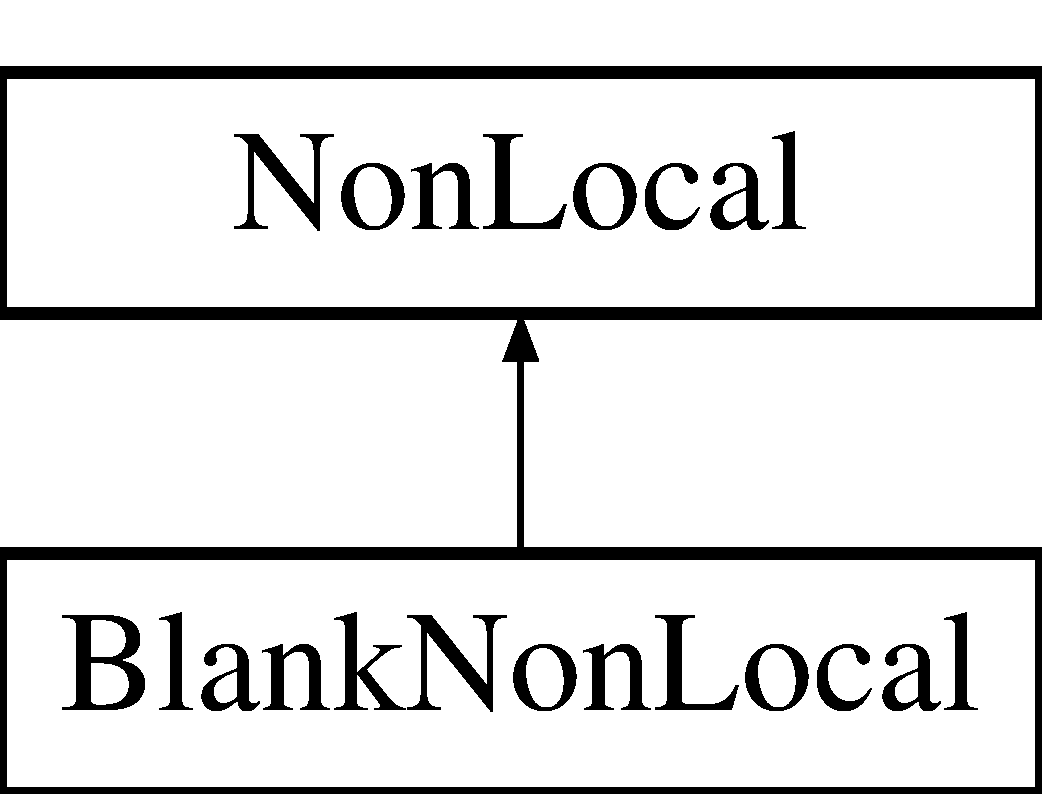
\includegraphics[height=2cm]{classBlankNonLocal}
\end{center}
\end{figure}
\subsection*{Public Member Functions}
\begin{DoxyCompactItemize}
\item 
\hypertarget{classBlankNonLocal_ab48fb9f176d5b929aaa724e3f5b32a6a}{
void {\bfseries compute} (const \hyperlink{classScarab_1_1HG_1_1Hyperedge}{Hyperedge} \&edge, const vector$<$ vector$<$ int $>$ $>$ \&subder, double \&score, vector$<$ int $>$ \&full\_\-derivation, Sig \&sig) const }
\label{classBlankNonLocal_ab48fb9f176d5b929aaa724e3f5b32a6a}

\item 
\hypertarget{classBlankNonLocal_a61e2ac11c599d217cacfa5c54bd191b8}{
virtual \hyperlink{structHyp}{Hyp} {\bfseries initialize} (const \hyperlink{classScarab_1_1HG_1_1Hypernode}{Hypernode} \&node) const }
\label{classBlankNonLocal_a61e2ac11c599d217cacfa5c54bd191b8}

\end{DoxyCompactItemize}


The documentation for this class was generated from the following file:\begin{DoxyCompactItemize}
\item 
hypergraph/CubePruning.h\end{DoxyCompactItemize}

\hypertarget{classCache}{
\section{Cache$<$ C, V $>$ Class Template Reference}
\label{classCache}\index{Cache@{Cache}}
}
\subsection*{Public Member Functions}
\begin{DoxyCompactItemize}
\item 
\hypertarget{classCache_ace98594381db6cd76b3228a73b18190a}{
{\bfseries Cache} (int size)}
\label{classCache_ace98594381db6cd76b3228a73b18190a}

\item 
\hypertarget{classCache_ad0a38f45b45b59a772d1e1fd92e59973}{
int {\bfseries size} ()}
\label{classCache_ad0a38f45b45b59a772d1e1fd92e59973}

\item 
\hypertarget{classCache_a8d126a64723abe79878befff1c622145}{
const V \& {\bfseries get} (const C \&edge) const }
\label{classCache_a8d126a64723abe79878befff1c622145}

\item 
\hypertarget{classCache_a2616bfc563def72da44f91977552ca62}{
V \& {\bfseries get\_\-no\_\-check} (const C \&edge)}
\label{classCache_a2616bfc563def72da44f91977552ca62}

\item 
\hypertarget{classCache_a9256aebb417928fbea6090f820d0652d}{
V \& {\bfseries get} (const C \&edge)}
\label{classCache_a9256aebb417928fbea6090f820d0652d}

\item 
\hypertarget{classCache_a509df0fde9598a4df9879b5ddb9d93d9}{
V {\bfseries get\_\-value} (const C \&edge) const }
\label{classCache_a509df0fde9598a4df9879b5ddb9d93d9}

\item 
\hypertarget{classCache_aeb9ab922add6cf79e2bef1b714f57e8a}{
void {\bfseries set\_\-value} (const C \&edge, V val)}
\label{classCache_aeb9ab922add6cf79e2bef1b714f57e8a}

\item 
\hypertarget{classCache_a0864be6a32d0840a4c3009f9ae417902}{
bool {\bfseries has\_\-key} (const C \&edge) const }
\label{classCache_a0864be6a32d0840a4c3009f9ae417902}

\item 
\hypertarget{classCache_a213273226c6bb403d33e10e2bc769fe1}{
bool {\bfseries has\_\-key} (int k) const }
\label{classCache_a213273226c6bb403d33e10e2bc769fe1}

\end{DoxyCompactItemize}
\subsection*{Public Attributes}
\begin{DoxyCompactItemize}
\item 
\hypertarget{classCache_a4de9009630d4bdc7e78b9db7ea734411}{
vector$<$ V $>$ {\bfseries store}}
\label{classCache_a4de9009630d4bdc7e78b9db7ea734411}

\item 
\hypertarget{classCache_a30fcdd51d6ff0cd602cc23d4a12b5348}{
vector$<$ bool $>$ {\bfseries has\_\-value}}
\label{classCache_a30fcdd51d6ff0cd602cc23d4a12b5348}

\end{DoxyCompactItemize}
\subsubsection*{template$<$class C, class V$>$ class Cache$<$ C, V $>$}



The documentation for this class was generated from the following file:\begin{DoxyCompactItemize}
\item 
hypergraph/EdgeCache.h\end{DoxyCompactItemize}

\hypertarget{structCandidate}{
\section{Candidate Struct Reference}
\label{structCandidate}\index{Candidate@{Candidate}}
}
\subsection*{Public Member Functions}
\begin{DoxyCompactItemize}
\item 
\hypertarget{structCandidate_ac13c7ec637d37b63fc4d6bf3361fd449}{
{\bfseries Candidate} (\hyperlink{structHyp}{Hyp} h, const \hyperlink{classScarab_1_1HG_1_1Hyperedge}{Hyperedge} \&e, const vector$<$ int $>$ \&v)}
\label{structCandidate_ac13c7ec637d37b63fc4d6bf3361fd449}

\item 
\hypertarget{structCandidate_a5644a3a3d2d92498923ecc443bb4583c}{
bool {\bfseries operator$<$} (const \hyperlink{structCandidate}{Candidate} \&other) const }
\label{structCandidate_a5644a3a3d2d92498923ecc443bb4583c}

\end{DoxyCompactItemize}
\subsection*{Public Attributes}
\begin{DoxyCompactItemize}
\item 
\hypertarget{structCandidate_a22db5a9c75fdebb31827505d6bc7d274}{
\hyperlink{structHyp}{Hyp} {\bfseries hyp}}
\label{structCandidate_a22db5a9c75fdebb31827505d6bc7d274}

\item 
\hypertarget{structCandidate_acdb6d12cbf33f6e78b97fed5013a181b}{
const \hyperlink{classScarab_1_1HG_1_1Hyperedge}{Hyperedge} \& {\bfseries edge}}
\label{structCandidate_acdb6d12cbf33f6e78b97fed5013a181b}

\item 
\hypertarget{structCandidate_afe2daf1c20513a5489d8407492ca7597}{
vector$<$ int $>$ {\bfseries vec}}
\label{structCandidate_afe2daf1c20513a5489d8407492ca7597}

\end{DoxyCompactItemize}


The documentation for this struct was generated from the following file:\begin{DoxyCompactItemize}
\item 
hypergraph/CubePruning.h\end{DoxyCompactItemize}

\hypertarget{structcandidate__compare}{
\section{candidate\_\-compare Struct Reference}
\label{structcandidate__compare}\index{candidate\_\-compare@{candidate\_\-compare}}
}
\subsection*{Public Member Functions}
\begin{DoxyCompactItemize}
\item 
\hypertarget{structcandidate__compare_ad142d42876f8dd88301ee5f1b3aed03b}{
bool {\bfseries operator()} (const \hyperlink{struct_candidate}{Candidate} $\ast$a, const \hyperlink{struct_candidate}{Candidate} $\ast$b) const }
\label{structcandidate__compare_ad142d42876f8dd88301ee5f1b3aed03b}

\end{DoxyCompactItemize}


The documentation for this struct was generated from the following file:\begin{DoxyCompactItemize}
\item 
hypergraph/CubePruning.h\end{DoxyCompactItemize}

\hypertarget{classClock}{
\section{Clock Class Reference}
\label{classClock}\index{Clock@{Clock}}
}
\subsection*{Static Public Member Functions}
\begin{DoxyCompactItemize}
\item 
\hypertarget{classClock_af45b8db844300755b8c4244a65f60833}{
static double {\bfseries diffclock} (clock\_\-t clock1, clock\_\-t clock2)}
\label{classClock_af45b8db844300755b8c4244a65f60833}

\end{DoxyCompactItemize}


The documentation for this class was generated from the following file:\begin{DoxyCompactItemize}
\item 
common.h\end{DoxyCompactItemize}

\hypertarget{classConstrainerDual}{
\section{ConstrainerDual Class Reference}
\label{classConstrainerDual}\index{ConstrainerDual@{ConstrainerDual}}
}
Inheritance diagram for ConstrainerDual:\begin{figure}[H]
\begin{center}
\leavevmode
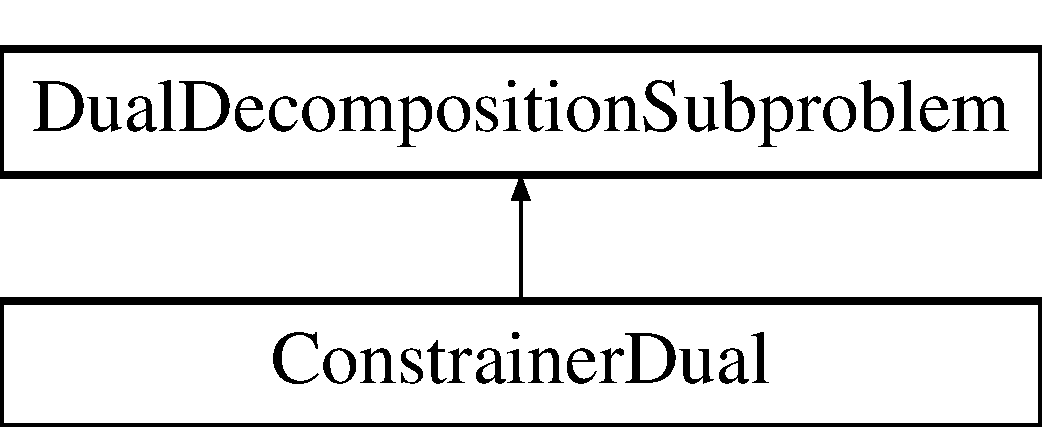
\includegraphics[height=2cm]{classConstrainerDual}
\end{center}
\end{figure}
\subsection*{Public Member Functions}
\begin{DoxyCompactItemize}
\item 
\hypertarget{classConstrainerDual_ae74adbb392415eec3451dd5a20820b6b}{
{\bfseries ConstrainerDual} (const \hyperlink{classTagConstraints}{TagConstraints} \&cons)}
\label{classConstrainerDual_ae74adbb392415eec3451dd5a20820b6b}

\item 
\hypertarget{classConstrainerDual_a8cd72c1288fc93a0fec014095ac7252b}{
void {\bfseries solve} (double \&primal, double \&dual, \hyperlink{classsvector}{wvector} \&, int)}
\label{classConstrainerDual_a8cd72c1288fc93a0fec014095ac7252b}

\item 
\hypertarget{classConstrainerDual_a622b99f704a3324133f08521eb4924f5}{
void {\bfseries update\_\-weights} (const \hyperlink{classsvector}{wvector} \&updates, \hyperlink{classsvector}{wvector} $\ast$weights, double mult)}
\label{classConstrainerDual_a622b99f704a3324133f08521eb4924f5}

\end{DoxyCompactItemize}
\subsection*{Protected Attributes}
\begin{DoxyCompactItemize}
\item 
\hypertarget{classConstrainerDual_abda18ff85d425d3748f49709534ec9ea}{
const \hyperlink{classTagConstraints}{TagConstraints} \& {\bfseries \_\-tag\_\-constraints}}
\label{classConstrainerDual_abda18ff85d425d3748f49709534ec9ea}

\item 
\hypertarget{classConstrainerDual_a4dd6e580712c0b35da77e42e137c7274}{
\hyperlink{classsvector}{wvector} $\ast$ {\bfseries \_\-cur\_\-weights}}
\label{classConstrainerDual_a4dd6e580712c0b35da77e42e137c7274}

\end{DoxyCompactItemize}


The documentation for this class was generated from the following files:\begin{DoxyCompactItemize}
\item 
tagger/TagSolvers.h\item 
tagger/TagSolvers.cpp\end{DoxyCompactItemize}

\hypertarget{classConstraintGroup}{
\section{ConstraintGroup Class Reference}
\label{classConstraintGroup}\index{ConstraintGroup@{ConstraintGroup}}
}
\subsection*{Public Member Functions}
\begin{DoxyCompactItemize}
\item 
\hypertarget{classConstraintGroup_a4f37823a56e405c16148c0ba6ae7f114}{
wvector {\bfseries solve\_\-hard} (wvector \&weights) const }
\label{classConstraintGroup_a4f37823a56e405c16148c0ba6ae7f114}

\end{DoxyCompactItemize}
\subsection*{Public Attributes}
\begin{DoxyCompactItemize}
\item 
\hypertarget{classConstraintGroup_ac96c45d3b2c4c1a6e1068837bc024d9c}{
vector$<$ \hyperlink{structPossibleTag}{PossibleTag} $>$ {\bfseries group}}
\label{classConstraintGroup_ac96c45d3b2c4c1a6e1068837bc024d9c}

\end{DoxyCompactItemize}


The documentation for this class was generated from the following files:\begin{DoxyCompactItemize}
\item 
tagger/TagConstraints.h\item 
tagger/TagConstraints.cpp\end{DoxyCompactItemize}

\hypertarget{classScarab_1_1HG_1_1Controller}{
\section{Scarab::HG::Controller Class Reference}
\label{classScarab_1_1HG_1_1Controller}\index{Scarab::HG::Controller@{Scarab::HG::Controller}}
}
Inheritance diagram for Scarab::HG::Controller:\begin{figure}[H]
\begin{center}
\leavevmode
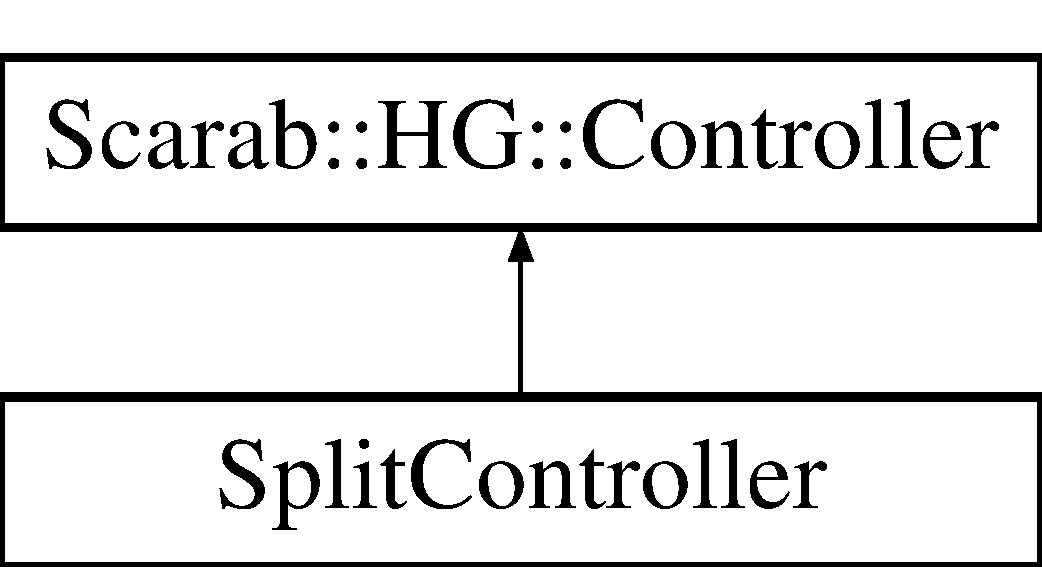
\includegraphics[height=2cm]{classScarab_1_1HG_1_1Controller}
\end{center}
\end{figure}
\subsection*{Public Member Functions}
\begin{DoxyCompactItemize}
\item 
double \hyperlink{classScarab_1_1HG_1_1Controller_a34cfe4b8e7496ffca1cedf64cb3f0a73}{combine} (const \hyperlink{structScarab_1_1HG_1_1Hypothesis}{Hypothesis} \&a, const \hyperlink{structScarab_1_1HG_1_1Hypothesis}{Hypothesis} \&b, \hyperlink{structScarab_1_1HG_1_1Hypothesis}{Hypothesis} \&ret) const 
\item 
\hypertarget{classScarab_1_1HG_1_1Controller_a4b596f04765ad11b691e29383f5fbc3b}{
double {\bfseries combine\_\-back} (const \hyperlink{structScarab_1_1HG_1_1Hypothesis}{Hypothesis} \&a, const \hyperlink{structScarab_1_1HG_1_1Hypothesis}{Hypothesis} \&b, \hyperlink{structScarab_1_1HG_1_1Hypothesis}{Hypothesis} \&ret) const }
\label{classScarab_1_1HG_1_1Controller_a4b596f04765ad11b691e29383f5fbc3b}

\item 
\hypertarget{classScarab_1_1HG_1_1Controller_a5019e9591e6d4e5e29eb4ca6ac42d056}{
virtual void {\bfseries initialize\_\-hypotheses} (const \hyperlink{classScarab_1_1HG_1_1Hypernode}{Hypernode} \&node, vector$<$ \hyperlink{structScarab_1_1HG_1_1Hypothesis}{Hypothesis} $\ast$ $>$ \&initialize, vector$<$ double $>$ \&scores) const =0}
\label{classScarab_1_1HG_1_1Controller_a5019e9591e6d4e5e29eb4ca6ac42d056}

\item 
\hypertarget{classScarab_1_1HG_1_1Controller_a34e4f087d77d06ee27fff2d3a8435473}{
virtual void {\bfseries initialize\_\-out\_\-root} (vector$<$ \hyperlink{structScarab_1_1HG_1_1Hypothesis}{Hypothesis} $\ast$ $>$ \&hyps, vector$<$ double $>$ \&scores) const =0}
\label{classScarab_1_1HG_1_1Controller_a34e4f087d77d06ee27fff2d3a8435473}

\item 
\hypertarget{classScarab_1_1HG_1_1Controller_ac4a38bf968379d3dc3f2b95cffabf540}{
virtual double {\bfseries find\_\-best} (vector$<$ \hyperlink{structScarab_1_1HG_1_1Hypothesis}{Hypothesis} $\ast$ $>$ \&at\_\-root, vector$<$ double $>$ \&scores, \hyperlink{structScarab_1_1HG_1_1Hypothesis}{Hypothesis} \&best\_\-hyp) const =0}
\label{classScarab_1_1HG_1_1Controller_ac4a38bf968379d3dc3f2b95cffabf540}

\item 
\hypertarget{classScarab_1_1HG_1_1Controller_a3498a09d093e6c6ed993e309db51480a}{
virtual int {\bfseries size} () const =0}
\label{classScarab_1_1HG_1_1Controller_a3498a09d093e6c6ed993e309db51480a}

\item 
\hypertarget{classScarab_1_1HG_1_1Controller_ab4282178c6b8d3670134ab0519eda518}{
virtual int {\bfseries dim} () const =0}
\label{classScarab_1_1HG_1_1Controller_ab4282178c6b8d3670134ab0519eda518}

\end{DoxyCompactItemize}


\subsection{Member Function Documentation}
\hypertarget{classScarab_1_1HG_1_1Controller_a34cfe4b8e7496ffca1cedf64cb3f0a73}{
\index{Scarab::HG::Controller@{Scarab::HG::Controller}!combine@{combine}}
\index{combine@{combine}!Scarab::HG::Controller@{Scarab::HG::Controller}}
\subsubsection[{combine}]{\setlength{\rightskip}{0pt plus 5cm}double Scarab::HG::Controller::combine (const {\bf Hypothesis} \& {\em a}, \/  const {\bf Hypothesis} \& {\em b}, \/  {\bf Hypothesis} \& {\em ret}) const\hspace{0.3cm}{\ttfamily  \mbox{[}inline\mbox{]}}}}
\label{classScarab_1_1HG_1_1Controller_a34cfe4b8e7496ffca1cedf64cb3f0a73}

\begin{DoxyParams}{Parameters}
\item[{\em a}]Left hypothesis \item[{\em b}]Right \hyperlink{structScarab_1_1HG_1_1Hypothesis}{Hypothesis} \item[{\em ret}]New constructed hypothesis\end{DoxyParams}
\begin{DoxyReturn}{Returns}
Added weight 
\end{DoxyReturn}


The documentation for this class was generated from the following file:\begin{DoxyCompactItemize}
\item 
hypergraph/Hypothesis.h\end{DoxyCompactItemize}

\hypertarget{classCubePruning}{
\section{CubePruning Class Reference}
\label{classCubePruning}\index{CubePruning@{CubePruning}}
}
\subsection*{Public Member Functions}
\begin{DoxyCompactItemize}
\item 
\hypertarget{classCubePruning_af17d9dda17f79a2c44b47501b9d99870}{
{\bfseries CubePruning} (const \hyperlink{classScarab_1_1HG_1_1HGraph}{HGraph} \&forest, const \hyperlink{classCache}{Cache}$<$ \hyperlink{classScarab_1_1HG_1_1Hyperedge}{Hyperedge}, double $>$ \&weights, const \hyperlink{classNonLocal}{NonLocal} \&non\_\-local, int k, int ratio)}
\label{classCubePruning_af17d9dda17f79a2c44b47501b9d99870}

\item 
\hypertarget{classCubePruning_a0e8d07fc09d695095be5b70780db95d6}{
void {\bfseries get\_\-derivation} (vector$<$ int $>$ \&der)}
\label{classCubePruning_a0e8d07fc09d695095be5b70780db95d6}

\item 
\hypertarget{classCubePruning_adf80c0c689d075765f250649433833e4}{
double {\bfseries parse} ()}
\label{classCubePruning_adf80c0c689d075765f250649433833e4}

\item 
\hypertarget{classCubePruning_ab949710c0d8e552cbadbe837b1b62d47}{
void {\bfseries run} (const \hyperlink{classScarab_1_1HG_1_1Hypernode}{Hypernode} \&cur\_\-node, vector$<$ \hyperlink{structHyp}{Hyp} $>$ \&kbest\_\-hyps)}
\label{classCubePruning_ab949710c0d8e552cbadbe837b1b62d47}

\item 
\hypertarget{classCubePruning_a14a4e797c638d07744dc328cf2ce568e}{
void {\bfseries init\_\-cube} (const \hyperlink{classScarab_1_1HG_1_1Hypernode}{Hypernode} \&cur\_\-node, Candidates \&cands)}
\label{classCubePruning_a14a4e797c638d07744dc328cf2ce568e}

\item 
\hypertarget{classCubePruning_abe8c53bd14fe4ad98ff6388f38a849cb}{
void {\bfseries kbest} (Candidates \&cands, vector$<$ \hyperlink{structHyp}{Hyp} $>$ \&)}
\label{classCubePruning_abe8c53bd14fe4ad98ff6388f38a849cb}

\item 
\hypertarget{classCubePruning_a5d3ab59862953b9000154e9c07c69634}{
void {\bfseries next} (const \hyperlink{classScarab_1_1HG_1_1Hyperedge}{Hyperedge} \&cedge, const vector$<$ int $>$ \&cvecj, Candidates \&cands)}
\label{classCubePruning_a5d3ab59862953b9000154e9c07c69634}

\item 
\hypertarget{classCubePruning_aa7d26357be4241b594f9eb24ac52da22}{
bool {\bfseries gethyp} (const \hyperlink{classScarab_1_1HG_1_1Hyperedge}{Hyperedge} \&cedge, const vector$<$ int $>$ \&vecj, \hyperlink{structHyp}{Hyp} \&item)}
\label{classCubePruning_aa7d26357be4241b594f9eb24ac52da22}

\end{DoxyCompactItemize}


The documentation for this class was generated from the following files:\begin{DoxyCompactItemize}
\item 
hypergraph/CubePruning.h\item 
hypergraph/CubePruning.cpp\end{DoxyCompactItemize}

\hypertarget{classDecode}{
\section{Decode Class Reference}
\label{classDecode}\index{Decode@{Decode}}
}
Inheritance diagram for Decode:\begin{figure}[H]
\begin{center}
\leavevmode
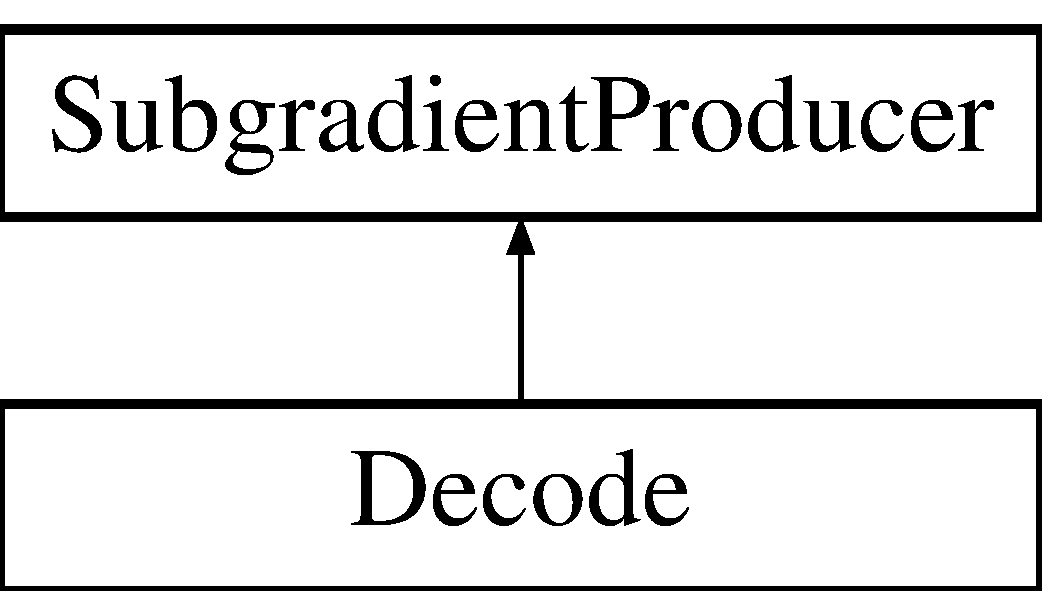
\includegraphics[height=2cm]{classDecode}
\end{center}
\end{figure}
\subsection*{Public Member Functions}
\begin{DoxyCompactItemize}
\item 
\hypertarget{classDecode_a57bd53ddaf49e2fe4b86a7aad782110f}{
{\bfseries Decode} (const \hyperlink{classForest}{Forest} \&forest, const \hyperlink{classForestLattice}{ForestLattice} \&lattice, const \hyperlink{classsvector}{wvector} \&weight, \hyperlink{classNgramCache}{NgramCache} \&lm)}
\label{classDecode_a57bd53ddaf49e2fe4b86a7aad782110f}

\item 
\hypertarget{classDecode_a6d86f91ee2c591c54ce2bb97c1dd6888}{
void {\bfseries solve} (double \&primal, double \&dual, \hyperlink{classsvector}{wvector} \&, int, bool, bool \&)}
\label{classDecode_a6d86f91ee2c591c54ce2bb97c1dd6888}

\item 
\hypertarget{classDecode_a9beca60221318f111b7f4d5acca8e329}{
void {\bfseries update\_\-weights} (const \hyperlink{classsvector}{wvector} \&updates, \hyperlink{classsvector}{wvector} $\ast$weights)}
\label{classDecode_a9beca60221318f111b7f4d5acca8e329}

\end{DoxyCompactItemize}


The documentation for this class was generated from the following files:\begin{DoxyCompactItemize}
\item 
trans\_\-decode/Decode.h\item 
trans\_\-decode/Decode.cpp\end{DoxyCompactItemize}

\hypertarget{classDep}{
\section{Dep Class Reference}
\label{classDep}\index{Dep@{Dep}}
}
\subsection*{Public Member Functions}
\begin{DoxyCompactItemize}
\item 
\hypertarget{classDep_a80362e936565b55abb269a18fde4dc59}{
{\bfseries Dep} (const \hyperlink{classDep}{Dep} \&from)}
\label{classDep_a80362e936565b55abb269a18fde4dc59}

\item 
\hypertarget{classDep_a87fdb64571ed9949e3fa5acdb9b367f9}{
\hyperlink{classDep}{Dep} \& {\bfseries operator=} (const \hyperlink{classDep}{Dep} \&from)}
\label{classDep_a87fdb64571ed9949e3fa5acdb9b367f9}

\item 
\hypertarget{classDep_a03cf321c0a637f65d4775ee8b63e2438}{
const ::google::protobuf::UnknownFieldSet \& {\bfseries unknown\_\-fields} () const }
\label{classDep_a03cf321c0a637f65d4775ee8b63e2438}

\item 
\hypertarget{classDep_af6070821655e8abd2054d0248896ed71}{
inline::google::protobuf::UnknownFieldSet $\ast$ {\bfseries mutable\_\-unknown\_\-fields} ()}
\label{classDep_af6070821655e8abd2054d0248896ed71}

\item 
\hypertarget{classDep_a89fd3d7654cbf49a112ee30ebe30a8f4}{
void {\bfseries Swap} (\hyperlink{classDep}{Dep} $\ast$other)}
\label{classDep_a89fd3d7654cbf49a112ee30ebe30a8f4}

\item 
\hypertarget{classDep_a27a82cb1d879df26d1cc89f5e10eacc2}{
\hyperlink{classDep}{Dep} $\ast$ {\bfseries New} () const }
\label{classDep_a27a82cb1d879df26d1cc89f5e10eacc2}

\item 
\hypertarget{classDep_a26c81c96d8bc499af3e3190127ae4f14}{
void {\bfseries CopyFrom} (const ::google::protobuf::Message \&from)}
\label{classDep_a26c81c96d8bc499af3e3190127ae4f14}

\item 
\hypertarget{classDep_a8521cee2d2c20cc3374caee792879d24}{
void {\bfseries MergeFrom} (const ::google::protobuf::Message \&from)}
\label{classDep_a8521cee2d2c20cc3374caee792879d24}

\item 
\hypertarget{classDep_a9c5e702a5cafd5a8bdf72ef36d754d27}{
void {\bfseries CopyFrom} (const \hyperlink{classDep}{Dep} \&from)}
\label{classDep_a9c5e702a5cafd5a8bdf72ef36d754d27}

\item 
\hypertarget{classDep_ad104b852e4e4e46eaa50d376b19fe83d}{
void {\bfseries MergeFrom} (const \hyperlink{classDep}{Dep} \&from)}
\label{classDep_ad104b852e4e4e46eaa50d376b19fe83d}

\item 
\hypertarget{classDep_a1713906a00ff37953c363bdbc07cbd54}{
void {\bfseries Clear} ()}
\label{classDep_a1713906a00ff37953c363bdbc07cbd54}

\item 
\hypertarget{classDep_ae39f86aae19b958824fd94b0092e07c9}{
bool {\bfseries IsInitialized} () const }
\label{classDep_ae39f86aae19b958824fd94b0092e07c9}

\item 
\hypertarget{classDep_af27fc8c7ab40a5ad63e3908db600fc5c}{
int {\bfseries ByteSize} () const }
\label{classDep_af27fc8c7ab40a5ad63e3908db600fc5c}

\item 
\hypertarget{classDep_a2080b72b2b01ff368d85506bfc311e28}{
bool {\bfseries MergePartialFromCodedStream} (::google::protobuf::io::CodedInputStream $\ast$input)}
\label{classDep_a2080b72b2b01ff368d85506bfc311e28}

\item 
\hypertarget{classDep_a1c5ffae565cd93485ba1b7de07678efc}{
void {\bfseries SerializeWithCachedSizes} (::google::protobuf::io::CodedOutputStream $\ast$output) const }
\label{classDep_a1c5ffae565cd93485ba1b7de07678efc}

\item 
\hypertarget{classDep_a7085fcc2588e12bc51d92f37682bba3b}{
::google::protobuf::uint8 $\ast$ {\bfseries SerializeWithCachedSizesToArray} (::google::protobuf::uint8 $\ast$output) const }
\label{classDep_a7085fcc2588e12bc51d92f37682bba3b}

\item 
\hypertarget{classDep_a0574f835da4e18501475c30e0b38ba20}{
int {\bfseries GetCachedSize} () const }
\label{classDep_a0574f835da4e18501475c30e0b38ba20}

\item 
\hypertarget{classDep_a4385e73adda64a977bae6d3304cd2a66}{
::google::protobuf::Metadata {\bfseries GetMetadata} () const }
\label{classDep_a4385e73adda64a977bae6d3304cd2a66}

\item 
\hypertarget{classDep_a7c31851d796bf8cb968b420fd07548cb}{
bool {\bfseries has\_\-head} () const }
\label{classDep_a7c31851d796bf8cb968b420fd07548cb}

\item 
\hypertarget{classDep_a32575258e5019204e6f4f53822181528}{
void {\bfseries clear\_\-head} ()}
\label{classDep_a32575258e5019204e6f4f53822181528}

\item 
\hypertarget{classDep_aebc1840c3493408ef316d45dec47e1a6}{
inline::google::protobuf::int32 {\bfseries head} () const }
\label{classDep_aebc1840c3493408ef316d45dec47e1a6}

\item 
\hypertarget{classDep_a43e73a016a5444b2e9f310eb0e2b671b}{
void {\bfseries set\_\-head} (::google::protobuf::int32 value)}
\label{classDep_a43e73a016a5444b2e9f310eb0e2b671b}

\item 
\hypertarget{classDep_a81b4aebd91b63196e503f80b3f1cb5d4}{
bool {\bfseries has\_\-mod} () const }
\label{classDep_a81b4aebd91b63196e503f80b3f1cb5d4}

\item 
\hypertarget{classDep_a286ffa524525424af7af0c509282b22c}{
void {\bfseries clear\_\-mod} ()}
\label{classDep_a286ffa524525424af7af0c509282b22c}

\item 
\hypertarget{classDep_a8b9785a6c223f1dcce0c1a0403bbb1dc}{
inline::google::protobuf::int32 {\bfseries mod} () const }
\label{classDep_a8b9785a6c223f1dcce0c1a0403bbb1dc}

\item 
\hypertarget{classDep_a3aa1f026840c0ec1631e4383399309f8}{
void {\bfseries set\_\-mod} (::google::protobuf::int32 value)}
\label{classDep_a3aa1f026840c0ec1631e4383399309f8}

\item 
\hypertarget{classDep_a80362e936565b55abb269a18fde4dc59}{
{\bfseries Dep} (const \hyperlink{classDep}{Dep} \&from)}
\label{classDep_a80362e936565b55abb269a18fde4dc59}

\item 
\hypertarget{classDep_a87fdb64571ed9949e3fa5acdb9b367f9}{
\hyperlink{classDep}{Dep} \& {\bfseries operator=} (const \hyperlink{classDep}{Dep} \&from)}
\label{classDep_a87fdb64571ed9949e3fa5acdb9b367f9}

\item 
\hypertarget{classDep_a03cf321c0a637f65d4775ee8b63e2438}{
const ::google::protobuf::UnknownFieldSet \& {\bfseries unknown\_\-fields} () const }
\label{classDep_a03cf321c0a637f65d4775ee8b63e2438}

\item 
\hypertarget{classDep_af6070821655e8abd2054d0248896ed71}{
inline::google::protobuf::UnknownFieldSet $\ast$ {\bfseries mutable\_\-unknown\_\-fields} ()}
\label{classDep_af6070821655e8abd2054d0248896ed71}

\item 
\hypertarget{classDep_a89fd3d7654cbf49a112ee30ebe30a8f4}{
void {\bfseries Swap} (\hyperlink{classDep}{Dep} $\ast$other)}
\label{classDep_a89fd3d7654cbf49a112ee30ebe30a8f4}

\item 
\hypertarget{classDep_add63de81fa6478b899aff7ae37b8dff1}{
\hyperlink{classDep}{Dep} $\ast$ {\bfseries New} () const }
\label{classDep_add63de81fa6478b899aff7ae37b8dff1}

\item 
\hypertarget{classDep_a26c81c96d8bc499af3e3190127ae4f14}{
void {\bfseries CopyFrom} (const ::google::protobuf::Message \&from)}
\label{classDep_a26c81c96d8bc499af3e3190127ae4f14}

\item 
\hypertarget{classDep_a8521cee2d2c20cc3374caee792879d24}{
void {\bfseries MergeFrom} (const ::google::protobuf::Message \&from)}
\label{classDep_a8521cee2d2c20cc3374caee792879d24}

\item 
\hypertarget{classDep_a9c5e702a5cafd5a8bdf72ef36d754d27}{
void {\bfseries CopyFrom} (const \hyperlink{classDep}{Dep} \&from)}
\label{classDep_a9c5e702a5cafd5a8bdf72ef36d754d27}

\item 
\hypertarget{classDep_ad104b852e4e4e46eaa50d376b19fe83d}{
void {\bfseries MergeFrom} (const \hyperlink{classDep}{Dep} \&from)}
\label{classDep_ad104b852e4e4e46eaa50d376b19fe83d}

\item 
\hypertarget{classDep_a1713906a00ff37953c363bdbc07cbd54}{
void {\bfseries Clear} ()}
\label{classDep_a1713906a00ff37953c363bdbc07cbd54}

\item 
\hypertarget{classDep_ae39f86aae19b958824fd94b0092e07c9}{
bool {\bfseries IsInitialized} () const }
\label{classDep_ae39f86aae19b958824fd94b0092e07c9}

\item 
\hypertarget{classDep_af27fc8c7ab40a5ad63e3908db600fc5c}{
int {\bfseries ByteSize} () const }
\label{classDep_af27fc8c7ab40a5ad63e3908db600fc5c}

\item 
\hypertarget{classDep_a2080b72b2b01ff368d85506bfc311e28}{
bool {\bfseries MergePartialFromCodedStream} (::google::protobuf::io::CodedInputStream $\ast$input)}
\label{classDep_a2080b72b2b01ff368d85506bfc311e28}

\item 
\hypertarget{classDep_a1c5ffae565cd93485ba1b7de07678efc}{
void {\bfseries SerializeWithCachedSizes} (::google::protobuf::io::CodedOutputStream $\ast$output) const }
\label{classDep_a1c5ffae565cd93485ba1b7de07678efc}

\item 
\hypertarget{classDep_a302a9df44af045d0f56ef4e14ee97816}{
::google::protobuf::uint8 $\ast$ {\bfseries SerializeWithCachedSizesToArray} (::google::protobuf::uint8 $\ast$output) const }
\label{classDep_a302a9df44af045d0f56ef4e14ee97816}

\item 
\hypertarget{classDep_a0574f835da4e18501475c30e0b38ba20}{
int {\bfseries GetCachedSize} () const }
\label{classDep_a0574f835da4e18501475c30e0b38ba20}

\item 
\hypertarget{classDep_acadc4712c5930d210c03df3d288358a9}{
::google::protobuf::Metadata {\bfseries GetMetadata} () const }
\label{classDep_acadc4712c5930d210c03df3d288358a9}

\item 
\hypertarget{classDep_a7c31851d796bf8cb968b420fd07548cb}{
bool {\bfseries has\_\-head} () const }
\label{classDep_a7c31851d796bf8cb968b420fd07548cb}

\item 
\hypertarget{classDep_a32575258e5019204e6f4f53822181528}{
void {\bfseries clear\_\-head} ()}
\label{classDep_a32575258e5019204e6f4f53822181528}

\item 
\hypertarget{classDep_aedebdf8b34a2f8f2705c3846e8ea78ed}{
inline::google::protobuf::int32 {\bfseries head} () const }
\label{classDep_aedebdf8b34a2f8f2705c3846e8ea78ed}

\item 
\hypertarget{classDep_a43e73a016a5444b2e9f310eb0e2b671b}{
void {\bfseries set\_\-head} (::google::protobuf::int32 value)}
\label{classDep_a43e73a016a5444b2e9f310eb0e2b671b}

\item 
\hypertarget{classDep_a81b4aebd91b63196e503f80b3f1cb5d4}{
bool {\bfseries has\_\-mod} () const }
\label{classDep_a81b4aebd91b63196e503f80b3f1cb5d4}

\item 
\hypertarget{classDep_a286ffa524525424af7af0c509282b22c}{
void {\bfseries clear\_\-mod} ()}
\label{classDep_a286ffa524525424af7af0c509282b22c}

\item 
\hypertarget{classDep_a53412c9bbc37fb2f0bbe124f8a131c72}{
inline::google::protobuf::int32 {\bfseries mod} () const }
\label{classDep_a53412c9bbc37fb2f0bbe124f8a131c72}

\item 
\hypertarget{classDep_a3aa1f026840c0ec1631e4383399309f8}{
void {\bfseries set\_\-mod} (::google::protobuf::int32 value)}
\label{classDep_a3aa1f026840c0ec1631e4383399309f8}

\end{DoxyCompactItemize}
\subsection*{Static Public Member Functions}
\begin{DoxyCompactItemize}
\item 
\hypertarget{classDep_af6a909e7ccf42b8c3b81cd01755a6f89}{
static const ::google::protobuf::Descriptor $\ast$ {\bfseries descriptor} ()}
\label{classDep_af6a909e7ccf42b8c3b81cd01755a6f89}

\item 
\hypertarget{classDep_adb231b00d2868737d7eed4a97c085c7b}{
static const \hyperlink{classDep}{Dep} \& {\bfseries default\_\-instance} ()}
\label{classDep_adb231b00d2868737d7eed4a97c085c7b}

\item 
\hypertarget{classDep_a29bfc132af3268c281ed5b2bfb7e09b5}{
static const ::google::protobuf::Descriptor $\ast$ {\bfseries descriptor} ()}
\label{classDep_a29bfc132af3268c281ed5b2bfb7e09b5}

\item 
\hypertarget{classDep_a81ccd4891740b599546e7e52c04ca516}{
static const \hyperlink{classDep}{Dep} \& {\bfseries default\_\-instance} ()}
\label{classDep_a81ccd4891740b599546e7e52c04ca516}

\end{DoxyCompactItemize}
\subsection*{Static Public Attributes}
\begin{DoxyCompactItemize}
\item 
\hypertarget{classDep_a30b9f1997de8bc996e1b0e1d5220dd99}{
static const int {\bfseries kHeadFieldNumber} = 1}
\label{classDep_a30b9f1997de8bc996e1b0e1d5220dd99}

\item 
\hypertarget{classDep_acb384371c72fcc36536bdb88a88cd05a}{
static const int {\bfseries kModFieldNumber} = 2}
\label{classDep_acb384371c72fcc36536bdb88a88cd05a}

\end{DoxyCompactItemize}
\subsection*{Friends}
\begin{DoxyCompactItemize}
\item 
\hypertarget{classDep_a2e2e426fb93c4aaa0e5b3d0a15899d92}{
void {\bfseries protobuf\_\-AddDesc\_\-dep\_\-2eproto} ()}
\label{classDep_a2e2e426fb93c4aaa0e5b3d0a15899d92}

\item 
\hypertarget{classDep_ae60899dfa8b3c6020f8e19070804c43b}{
void {\bfseries protobuf\_\-AssignDesc\_\-dep\_\-2eproto} ()}
\label{classDep_ae60899dfa8b3c6020f8e19070804c43b}

\item 
\hypertarget{classDep_aab3c3b65c9043a8a41dcb95f310b49e8}{
void {\bfseries protobuf\_\-ShutdownFile\_\-dep\_\-2eproto} ()}
\label{classDep_aab3c3b65c9043a8a41dcb95f310b49e8}

\item 
\hypertarget{classDep_a2e2e426fb93c4aaa0e5b3d0a15899d92}{
void {\bfseries protobuf\_\-AddDesc\_\-dep\_\-2eproto} ()}
\label{classDep_a2e2e426fb93c4aaa0e5b3d0a15899d92}

\item 
\hypertarget{classDep_ae60899dfa8b3c6020f8e19070804c43b}{
void {\bfseries protobuf\_\-AssignDesc\_\-dep\_\-2eproto} ()}
\label{classDep_ae60899dfa8b3c6020f8e19070804c43b}

\item 
\hypertarget{classDep_aab3c3b65c9043a8a41dcb95f310b49e8}{
void {\bfseries protobuf\_\-ShutdownFile\_\-dep\_\-2eproto} ()}
\label{classDep_aab3c3b65c9043a8a41dcb95f310b49e8}

\end{DoxyCompactItemize}


The documentation for this class was generated from the following files:\begin{DoxyCompactItemize}
\item 
interfaces/hypergraph/gen-\/cpp/dep.pb.h\item 
interfaces/hypergraph/gen\_\-cpp/dep.pb.h\item 
interfaces/hypergraph/gen-\/cpp/dep.pb.cc\item 
interfaces/hypergraph/gen\_\-cpp/dep.pb.cc\end{DoxyCompactItemize}

\hypertarget{structDependency}{
\section{Dependency Struct Reference}
\label{structDependency}\index{Dependency@{Dependency}}
}
\subsection*{Public Member Functions}
\begin{DoxyCompactItemize}
\item 
\hypertarget{structDependency_a92ebdf715c4c81e556bc274f86027400}{
{\bfseries Dependency} (int l, int h, int m)}
\label{structDependency_a92ebdf715c4c81e556bc274f86027400}

\item 
\hypertarget{structDependency_a38ba361a116c72f4e41298b6320a6540}{
int {\bfseries id} () const }
\label{structDependency_a38ba361a116c72f4e41298b6320a6540}

\end{DoxyCompactItemize}
\subsection*{Public Attributes}
\begin{DoxyCompactItemize}
\item 
\hypertarget{structDependency_ae50c91ea1c7f2a16a29e7ecf9cf0a6ba}{
int {\bfseries head}}
\label{structDependency_ae50c91ea1c7f2a16a29e7ecf9cf0a6ba}

\item 
\hypertarget{structDependency_a45e806cfc00a3bcce4d5ebaab52c1f77}{
int {\bfseries mod}}
\label{structDependency_a45e806cfc00a3bcce4d5ebaab52c1f77}

\item 
\hypertarget{structDependency_a95f049533781d9ae8fea8f447e4739fe}{
int {\bfseries length}}
\label{structDependency_a95f049533781d9ae8fea8f447e4739fe}

\end{DoxyCompactItemize}


The documentation for this struct was generated from the following file:\begin{DoxyCompactItemize}
\item 
parse/DepParser.h\end{DoxyCompactItemize}

\hypertarget{classDepParser}{
\section{DepParser Class Reference}
\label{classDepParser}\index{DepParser@{DepParser}}
}
Inheritance diagram for DepParser:\begin{figure}[H]
\begin{center}
\leavevmode
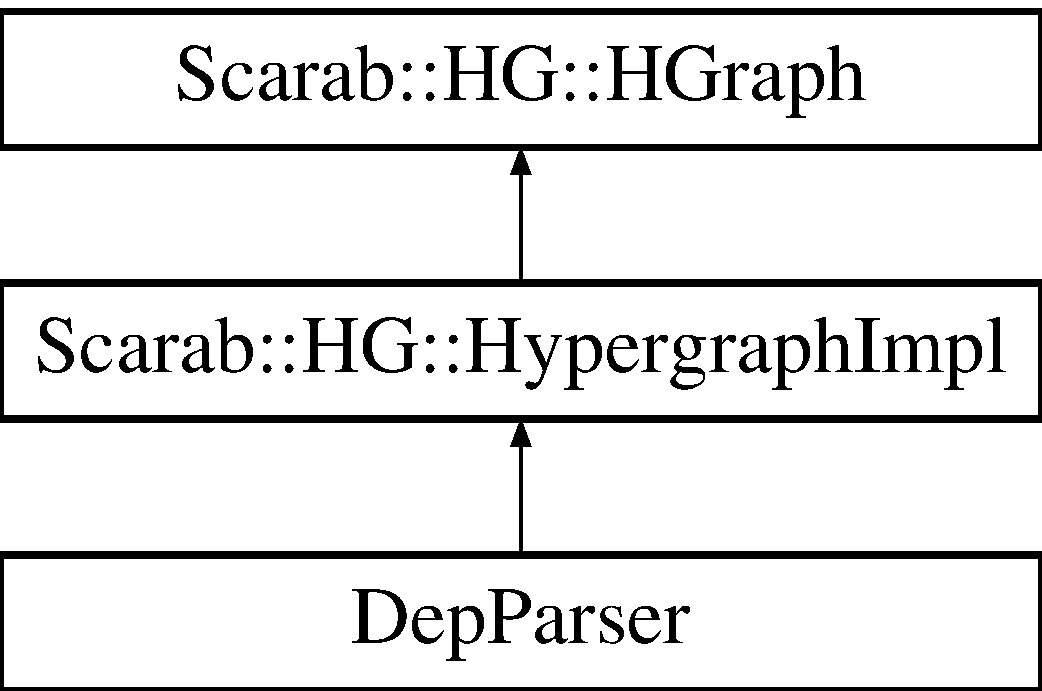
\includegraphics[height=3cm]{classDepParser}
\end{center}
\end{figure}
\subsection*{Public Member Functions}
\begin{DoxyCompactItemize}
\item 
void \hyperlink{classDepParser_a9aebbbde821bad423b6c01cc12f02a2c}{print} () const 
\item 
\hypertarget{classDepParser_a6131e95a8ec7b07f7a4d68dae224d52f}{
void {\bfseries set\_\-up} (const Hypergraph \&hgraph)}
\label{classDepParser_a6131e95a8ec7b07f7a4d68dae224d52f}

\item 
\hypertarget{classDepParser_aaec31758432c2d3336d2164996571688}{
const Hypergraph \& {\bfseries hypergraph} () const }
\label{classDepParser_aaec31758432c2d3336d2164996571688}

\item 
\hypertarget{classDepParser_aa64f67830bf4c3bf9936ba6056dfdff0}{
vector$<$ \hyperlink{structDependency}{Dependency} $>$ {\bfseries dependencies} () const }
\label{classDepParser_aa64f67830bf4c3bf9936ba6056dfdff0}

\item 
\hypertarget{classDepParser_aaff55cf38fd9b1fbfb22090ddeb72ba8}{
uint {\bfseries num\_\-deps} () const }
\label{classDepParser_aaff55cf38fd9b1fbfb22090ddeb72ba8}

\item 
\hypertarget{classDepParser_a86b99d09d76b7d6f8733b208e9f32822}{
uint {\bfseries sent\_\-length} () const }
\label{classDepParser_a86b99d09d76b7d6f8733b208e9f32822}

\item 
\hypertarget{classDepParser_a49afcb1a83a3c924869faf34cd9e968e}{
\hyperlink{structDependency}{Dependency} {\bfseries make\_\-dep} (int head, int mod) const }
\label{classDepParser_a49afcb1a83a3c924869faf34cd9e968e}

\item 
\hypertarget{classDepParser_a9fa2f0bf24cd870404f0a99b5926c558}{
const vector$<$ const \hyperlink{classScarab_1_1HG_1_1Hyperedge}{Hyperedge} $\ast$ $>$ \& {\bfseries dep\_\-to\_\-edge} (const \hyperlink{structDependency}{Dependency} \&dep) const }
\label{classDepParser_a9fa2f0bf24cd870404f0a99b5926c558}

\item 
\hypertarget{classDepParser_aa5ff87f99326c60633fb8e26d1737776}{
const \hyperlink{structDependency}{Dependency} \& {\bfseries edge\_\-to\_\-dep} (const \hyperlink{classScarab_1_1HG_1_1Hyperedge}{Hyperedge} \&edge) const }
\label{classDepParser_aa5ff87f99326c60633fb8e26d1737776}

\item 
\hypertarget{classDepParser_abd0b9171e59c1c40cdb58807a46a5449}{
bool {\bfseries edge\_\-has\_\-dep} (const \hyperlink{classScarab_1_1HG_1_1Hyperedge}{Hyperedge} \&edge) const }
\label{classDepParser_abd0b9171e59c1c40cdb58807a46a5449}

\end{DoxyCompactItemize}
\subsection*{Protected Member Functions}
\begin{DoxyCompactItemize}
\item 
\hypertarget{classDepParser_a04d313d931d1e8b0bac3a36ca7be469b}{
void {\bfseries make\_\-edge} (const Hypergraph\_\-Edge \&edge, const \hyperlink{classScarab_1_1HG_1_1Hyperedge}{Scarab::HG::Hyperedge} $\ast$our\_\-edge)}
\label{classDepParser_a04d313d931d1e8b0bac3a36ca7be469b}

\end{DoxyCompactItemize}


\subsection{Member Function Documentation}
\hypertarget{classDepParser_a9aebbbde821bad423b6c01cc12f02a2c}{
\index{DepParser@{DepParser}!print@{print}}
\index{print@{print}!DepParser@{DepParser}}
\subsubsection[{print}]{\setlength{\rightskip}{0pt plus 5cm}void DepParser::print () const\hspace{0.3cm}{\ttfamily  \mbox{[}inline, virtual\mbox{]}}}}
\label{classDepParser_a9aebbbde821bad423b6c01cc12f02a2c}
Display the hypergraph for debugging. 

Implements \hyperlink{classScarab_1_1HG_1_1HGraph_ab5aa11c932b28864b56f28e0babbc1c1}{Scarab::HG::HGraph}.



The documentation for this class was generated from the following file:\begin{DoxyCompactItemize}
\item 
parse/DepParser.h\end{DoxyCompactItemize}

\hypertarget{structScarab_1_1HG_1_1DepParserLP}{
\section{Scarab::HG::DepParserLP Struct Reference}
\label{structScarab_1_1HG_1_1DepParserLP}\index{Scarab::HG::DepParserLP@{Scarab::HG::DepParserLP}}
}
\subsection*{Public Member Functions}
\begin{DoxyCompactItemize}
\item 
\hypertarget{structScarab_1_1HG_1_1DepParserLP_aaec1248e50de35594c4a20e89a782e95}{
{\bfseries DepParserLP} (const \hyperlink{classDepParser}{DepParser} \&parser, const \hyperlink{structScarab_1_1HG_1_1HypergraphLP}{HypergraphLP} \&hyper\_\-lp)}
\label{structScarab_1_1HG_1_1DepParserLP_aaec1248e50de35594c4a20e89a782e95}

\end{DoxyCompactItemize}
\subsection*{Public Attributes}
\begin{DoxyCompactItemize}
\item 
\hypertarget{structScarab_1_1HG_1_1DepParserLP_af31e9d91e3407559cd2588bfef2296e3}{
\hyperlink{classCache}{Cache}$<$ \hyperlink{structDependency}{Dependency}, GRBVar $>$ {\bfseries dep\_\-vars}}
\label{structScarab_1_1HG_1_1DepParserLP_af31e9d91e3407559cd2588bfef2296e3}

\item 
\hypertarget{structScarab_1_1HG_1_1DepParserLP_a93d0f269dabdd6fe83c68ee51baafb62}{
const \hyperlink{classDepParser}{DepParser} \& {\bfseries p}}
\label{structScarab_1_1HG_1_1DepParserLP_a93d0f269dabdd6fe83c68ee51baafb62}

\item 
\hypertarget{structScarab_1_1HG_1_1DepParserLP_acab7463a0d1349c5a1250ac0653c0569}{
const \hyperlink{structScarab_1_1HG_1_1HypergraphLP}{HypergraphLP} \& {\bfseries h\_\-lp}}
\label{structScarab_1_1HG_1_1DepParserLP_acab7463a0d1349c5a1250ac0653c0569}

\end{DoxyCompactItemize}


The documentation for this struct was generated from the following file:\begin{DoxyCompactItemize}
\item 
lp/DepParseLP.h\end{DoxyCompactItemize}

\hypertarget{classScarab_1_1HG_1_1DepParserLPBuilder}{
\section{Scarab::HG::DepParserLPBuilder Class Reference}
\label{classScarab_1_1HG_1_1DepParserLPBuilder}\index{Scarab::HG::DepParserLPBuilder@{Scarab::HG::DepParserLPBuilder}}
}
\subsection*{Static Public Member Functions}
\begin{DoxyCompactItemize}
\item 
\hypertarget{classScarab_1_1HG_1_1DepParserLPBuilder_a8864b215a93fa51c4df30669dacb0ddc}{
static void {\bfseries show\_\-results} (const \hyperlink{structScarab_1_1HG_1_1DepParserLP}{DepParserLP} \&lp\_\-vars)}
\label{classScarab_1_1HG_1_1DepParserLPBuilder_a8864b215a93fa51c4df30669dacb0ddc}

\item 
\hypertarget{classScarab_1_1HG_1_1DepParserLPBuilder_a862127f9347f244103941a119747b810}{
static \hyperlink{structScarab_1_1HG_1_1DepParserLP}{DepParserLP} $\ast$ {\bfseries add\_\-parse} (const \hyperlink{classDepParser}{DepParser} \&parser, const \hyperlink{classCache}{Cache}$<$ \hyperlink{classScarab_1_1HG_1_1Hyperedge}{Hyperedge}, double $>$ \&weights, string prefix, GRBModel \&model, int var\_\-type)}
\label{classScarab_1_1HG_1_1DepParserLPBuilder_a862127f9347f244103941a119747b810}

\end{DoxyCompactItemize}


The documentation for this class was generated from the following files:\begin{DoxyCompactItemize}
\item 
lp/DepParseLP.h\item 
lp/DepParseLP.cpp\end{DoxyCompactItemize}

\hypertarget{classDualDecomposition}{
\section{DualDecomposition Class Reference}
\label{classDualDecomposition}\index{DualDecomposition@{DualDecomposition}}
}
\subsection*{Public Member Functions}
\begin{DoxyCompactItemize}
\item 
\hypertarget{classDualDecomposition_a652c2229bad83ce7b135aa06ef1283a5}{
{\bfseries DualDecomposition} (\hyperlink{classDualDecompositionSubproblem}{DualDecompositionSubproblem} \&s1, \hyperlink{classDualDecompositionSubproblem}{DualDecompositionSubproblem} \&s2)}
\label{classDualDecomposition_a652c2229bad83ce7b135aa06ef1283a5}

\item 
\hypertarget{classDualDecomposition_a0013544261cba254dc2ca2c68cbb1679}{
void {\bfseries solve} (int example)}
\label{classDualDecomposition_a0013544261cba254dc2ca2c68cbb1679}

\end{DoxyCompactItemize}


The documentation for this class was generated from the following file:\begin{DoxyCompactItemize}
\item 
optimization/DualDecomposition.h\end{DoxyCompactItemize}

\hypertarget{classDualDecompositionRunner}{
\section{DualDecompositionRunner Class Reference}
\label{classDualDecompositionRunner}\index{DualDecompositionRunner@{DualDecompositionRunner}}
}
Inheritance diagram for DualDecompositionRunner:\begin{figure}[H]
\begin{center}
\leavevmode
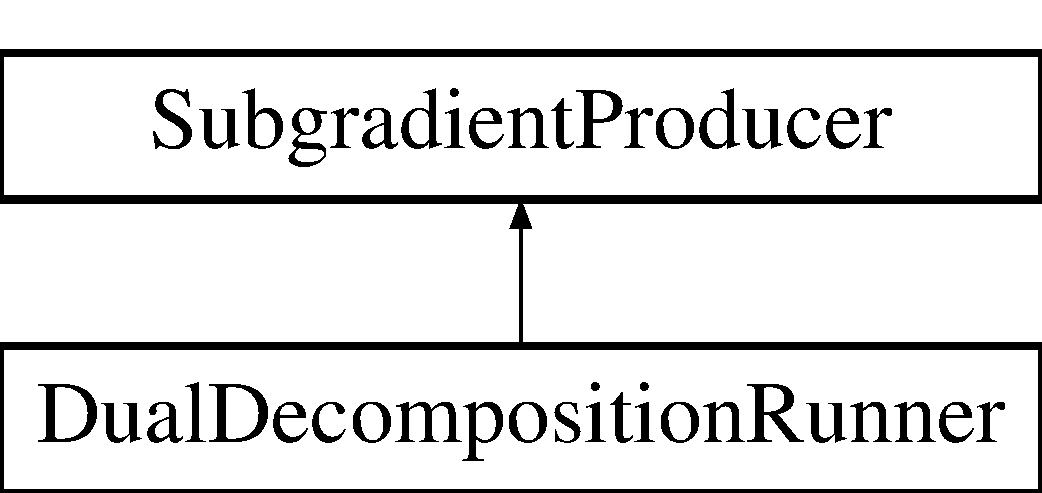
\includegraphics[height=2cm]{classDualDecompositionRunner}
\end{center}
\end{figure}
\subsection*{Public Member Functions}
\begin{DoxyCompactItemize}
\item 
\hypertarget{classDualDecompositionRunner_ad0af4c8b1a73612770d329cf560af9d1}{
{\bfseries DualDecompositionRunner} (\hyperlink{classDualDecompositionSubproblem}{DualDecompositionSubproblem} \&s1, \hyperlink{classDualDecompositionSubproblem}{DualDecompositionSubproblem} \&s2)}
\label{classDualDecompositionRunner_ad0af4c8b1a73612770d329cf560af9d1}

\item 
\hypertarget{classDualDecompositionRunner_a4bcec895359acf32000d42155c4593ef}{
void {\bfseries solve} (double \&primal, double \&dual, wvector \&subgrad, int round, bool is\_\-stuck, bool \&bump\_\-rate)}
\label{classDualDecompositionRunner_a4bcec895359acf32000d42155c4593ef}

\item 
\hypertarget{classDualDecompositionRunner_a3cdf7ce33f6454f9fee9fb9c3287c5ac}{
void {\bfseries update\_\-weights} (const wvector \&updates, wvector $\ast$weights)}
\label{classDualDecompositionRunner_a3cdf7ce33f6454f9fee9fb9c3287c5ac}

\end{DoxyCompactItemize}
\subsection*{Public Attributes}
\begin{DoxyCompactItemize}
\item 
\hypertarget{classDualDecompositionRunner_a13371fbf1e5109e8a9d920d2ed0b7bea}{
\hyperlink{classDualDecompositionSubproblem}{DualDecompositionSubproblem} \& {\bfseries \_\-sub\_\-producer1}}
\label{classDualDecompositionRunner_a13371fbf1e5109e8a9d920d2ed0b7bea}

\item 
\hypertarget{classDualDecompositionRunner_a988b68df84c131bc47d142ae8638fbd1}{
\hyperlink{classDualDecompositionSubproblem}{DualDecompositionSubproblem} \& {\bfseries \_\-sub\_\-producer2}}
\label{classDualDecompositionRunner_a988b68df84c131bc47d142ae8638fbd1}

\end{DoxyCompactItemize}


The documentation for this class was generated from the following file:\begin{DoxyCompactItemize}
\item 
optimization/DualDecomposition.h\end{DoxyCompactItemize}

\hypertarget{classDualDecompositionSubproblem}{
\section{DualDecompositionSubproblem Class Reference}
\label{classDualDecompositionSubproblem}\index{DualDecompositionSubproblem@{DualDecompositionSubproblem}}
}
Inheritance diagram for DualDecompositionSubproblem:\begin{figure}[H]
\begin{center}
\leavevmode
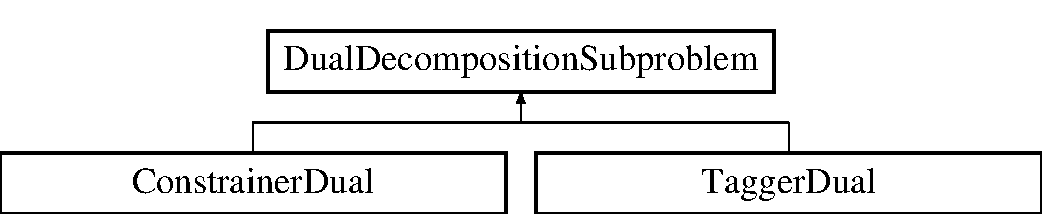
\includegraphics[height=2cm]{classDualDecompositionSubproblem}
\end{center}
\end{figure}
\subsection*{Public Member Functions}
\begin{DoxyCompactItemize}
\item 
\hypertarget{classDualDecompositionSubproblem_aac234786c13091898be348dc0056a036}{
virtual void {\bfseries solve} (double \&primal, double \&dual, \hyperlink{classsvector}{wvector} \&, int)=0}
\label{classDualDecompositionSubproblem_aac234786c13091898be348dc0056a036}

\item 
\hypertarget{classDualDecompositionSubproblem_a6d26fcb23023d5b03d54b3d191531b02}{
virtual void {\bfseries update\_\-weights} (const \hyperlink{classsvector}{wvector} \&updates, \hyperlink{classsvector}{wvector} $\ast$weights, double mult)=0}
\label{classDualDecompositionSubproblem_a6d26fcb23023d5b03d54b3d191531b02}

\end{DoxyCompactItemize}


The documentation for this class was generated from the following file:\begin{DoxyCompactItemize}
\item 
optimization/DualDecomposition.h\end{DoxyCompactItemize}

\hypertarget{classgraph_1_1EdgeStatePotential}{
\section{graph::EdgeStatePotential Class Reference}
\label{classgraph_1_1EdgeStatePotential}\index{graph::EdgeStatePotential@{graph::EdgeStatePotential}}
}
\subsection*{Public Member Functions}
\begin{DoxyCompactItemize}
\item 
\hypertarget{classgraph_1_1EdgeStatePotential_a07c6b74b96e49c9dd58dd6801d331734}{
{\bfseries EdgeStatePotential} (const \hyperlink{classgraph_1_1EdgeStatePotential}{EdgeStatePotential} \&from)}
\label{classgraph_1_1EdgeStatePotential_a07c6b74b96e49c9dd58dd6801d331734}

\item 
\hypertarget{classgraph_1_1EdgeStatePotential_aa84be9ac7930900ea711dd50c61a992c}{
\hyperlink{classgraph_1_1EdgeStatePotential}{EdgeStatePotential} \& {\bfseries operator=} (const \hyperlink{classgraph_1_1EdgeStatePotential}{EdgeStatePotential} \&from)}
\label{classgraph_1_1EdgeStatePotential_aa84be9ac7930900ea711dd50c61a992c}

\item 
\hypertarget{classgraph_1_1EdgeStatePotential_aa3d87d59c31b9583a2723bf7d838b7e8}{
const ::google::protobuf::UnknownFieldSet \& {\bfseries unknown\_\-fields} () const }
\label{classgraph_1_1EdgeStatePotential_aa3d87d59c31b9583a2723bf7d838b7e8}

\item 
\hypertarget{classgraph_1_1EdgeStatePotential_ade01e66023e544434ec77933186df507}{
inline::google::protobuf::UnknownFieldSet $\ast$ {\bfseries mutable\_\-unknown\_\-fields} ()}
\label{classgraph_1_1EdgeStatePotential_ade01e66023e544434ec77933186df507}

\item 
\hypertarget{classgraph_1_1EdgeStatePotential_ae27775781654c45f108db1186e4702a7}{
void {\bfseries Swap} (\hyperlink{classgraph_1_1EdgeStatePotential}{EdgeStatePotential} $\ast$other)}
\label{classgraph_1_1EdgeStatePotential_ae27775781654c45f108db1186e4702a7}

\item 
\hypertarget{classgraph_1_1EdgeStatePotential_abcc4686ae346371daef72453939d9897}{
\hyperlink{classgraph_1_1EdgeStatePotential}{EdgeStatePotential} $\ast$ {\bfseries New} () const }
\label{classgraph_1_1EdgeStatePotential_abcc4686ae346371daef72453939d9897}

\item 
\hypertarget{classgraph_1_1EdgeStatePotential_ac83756fba5134e67c234a0d6f647588d}{
void {\bfseries CopyFrom} (const ::google::protobuf::Message \&from)}
\label{classgraph_1_1EdgeStatePotential_ac83756fba5134e67c234a0d6f647588d}

\item 
\hypertarget{classgraph_1_1EdgeStatePotential_a66c8261423f9120136fb74142cd47483}{
void {\bfseries MergeFrom} (const ::google::protobuf::Message \&from)}
\label{classgraph_1_1EdgeStatePotential_a66c8261423f9120136fb74142cd47483}

\item 
\hypertarget{classgraph_1_1EdgeStatePotential_a8f55d319916f544ccef4671d036dac9e}{
void {\bfseries CopyFrom} (const \hyperlink{classgraph_1_1EdgeStatePotential}{EdgeStatePotential} \&from)}
\label{classgraph_1_1EdgeStatePotential_a8f55d319916f544ccef4671d036dac9e}

\item 
\hypertarget{classgraph_1_1EdgeStatePotential_abff176deb7b6e4934b2d7cd4d4b1bcf0}{
void {\bfseries MergeFrom} (const \hyperlink{classgraph_1_1EdgeStatePotential}{EdgeStatePotential} \&from)}
\label{classgraph_1_1EdgeStatePotential_abff176deb7b6e4934b2d7cd4d4b1bcf0}

\item 
\hypertarget{classgraph_1_1EdgeStatePotential_a83c0c837389b1ae8f84bcb894022ae35}{
void {\bfseries Clear} ()}
\label{classgraph_1_1EdgeStatePotential_a83c0c837389b1ae8f84bcb894022ae35}

\item 
\hypertarget{classgraph_1_1EdgeStatePotential_a6f9a1a9fb84714dee4bf5b4b24494ead}{
bool {\bfseries IsInitialized} () const }
\label{classgraph_1_1EdgeStatePotential_a6f9a1a9fb84714dee4bf5b4b24494ead}

\item 
\hypertarget{classgraph_1_1EdgeStatePotential_a0a60ec89c3fcf88ec83e01bcc5d89279}{
int {\bfseries ByteSize} () const }
\label{classgraph_1_1EdgeStatePotential_a0a60ec89c3fcf88ec83e01bcc5d89279}

\item 
\hypertarget{classgraph_1_1EdgeStatePotential_adfc707ab77b2d69e5ed5f4770ed3f680}{
bool {\bfseries MergePartialFromCodedStream} (::google::protobuf::io::CodedInputStream $\ast$input)}
\label{classgraph_1_1EdgeStatePotential_adfc707ab77b2d69e5ed5f4770ed3f680}

\item 
\hypertarget{classgraph_1_1EdgeStatePotential_ad02fa972c66749f49ce34430af59a2b9}{
void {\bfseries SerializeWithCachedSizes} (::google::protobuf::io::CodedOutputStream $\ast$output) const }
\label{classgraph_1_1EdgeStatePotential_ad02fa972c66749f49ce34430af59a2b9}

\item 
\hypertarget{classgraph_1_1EdgeStatePotential_a33c5ffdfb724a6abafecd982ea9d2f1d}{
::google::protobuf::uint8 $\ast$ {\bfseries SerializeWithCachedSizesToArray} (::google::protobuf::uint8 $\ast$output) const }
\label{classgraph_1_1EdgeStatePotential_a33c5ffdfb724a6abafecd982ea9d2f1d}

\item 
\hypertarget{classgraph_1_1EdgeStatePotential_acd032f41037bb2d600aead1931aba43c}{
int {\bfseries GetCachedSize} () const }
\label{classgraph_1_1EdgeStatePotential_acd032f41037bb2d600aead1931aba43c}

\item 
\hypertarget{classgraph_1_1EdgeStatePotential_aedd1ff1e5220e39f32e629f39747e22a}{
::google::protobuf::Metadata {\bfseries GetMetadata} () const }
\label{classgraph_1_1EdgeStatePotential_aedd1ff1e5220e39f32e629f39747e22a}

\item 
\hypertarget{classgraph_1_1EdgeStatePotential_a5f9ee1db6bb4e2db964624974a6c506f}{
bool {\bfseries has\_\-from\_\-state\_\-id} () const }
\label{classgraph_1_1EdgeStatePotential_a5f9ee1db6bb4e2db964624974a6c506f}

\item 
\hypertarget{classgraph_1_1EdgeStatePotential_a5a02ced96b71190c158d0fb81bf00fd5}{
void {\bfseries clear\_\-from\_\-state\_\-id} ()}
\label{classgraph_1_1EdgeStatePotential_a5a02ced96b71190c158d0fb81bf00fd5}

\item 
\hypertarget{classgraph_1_1EdgeStatePotential_adcdf4b14113ac0259bafb2bf142d19f0}{
inline::google::protobuf::int32 {\bfseries from\_\-state\_\-id} () const }
\label{classgraph_1_1EdgeStatePotential_adcdf4b14113ac0259bafb2bf142d19f0}

\item 
\hypertarget{classgraph_1_1EdgeStatePotential_ab23b81819bc6d9dd71d319c49412c8d8}{
void {\bfseries set\_\-from\_\-state\_\-id} (::google::protobuf::int32 value)}
\label{classgraph_1_1EdgeStatePotential_ab23b81819bc6d9dd71d319c49412c8d8}

\item 
\hypertarget{classgraph_1_1EdgeStatePotential_a1c2e8dc8b84f5aacf08e5c46866f04c6}{
bool {\bfseries has\_\-to\_\-state\_\-id} () const }
\label{classgraph_1_1EdgeStatePotential_a1c2e8dc8b84f5aacf08e5c46866f04c6}

\item 
\hypertarget{classgraph_1_1EdgeStatePotential_a7f30d4b4ff6eb1c6695799be4eeefea5}{
void {\bfseries clear\_\-to\_\-state\_\-id} ()}
\label{classgraph_1_1EdgeStatePotential_a7f30d4b4ff6eb1c6695799be4eeefea5}

\item 
\hypertarget{classgraph_1_1EdgeStatePotential_acdc19ad89d3da217371556b1d069a971}{
inline::google::protobuf::int32 {\bfseries to\_\-state\_\-id} () const }
\label{classgraph_1_1EdgeStatePotential_acdc19ad89d3da217371556b1d069a971}

\item 
\hypertarget{classgraph_1_1EdgeStatePotential_ad498cc27a96c02d74bc44718f289771c}{
void {\bfseries set\_\-to\_\-state\_\-id} (::google::protobuf::int32 value)}
\label{classgraph_1_1EdgeStatePotential_ad498cc27a96c02d74bc44718f289771c}

\item 
\hypertarget{classgraph_1_1EdgeStatePotential_a74db33f4d6408cb2f00a4c02d5b8d492}{
bool {\bfseries has\_\-edge\_\-potential} () const }
\label{classgraph_1_1EdgeStatePotential_a74db33f4d6408cb2f00a4c02d5b8d492}

\item 
\hypertarget{classgraph_1_1EdgeStatePotential_a8962a3e1a075a505dc2b212dd0308791}{
void {\bfseries clear\_\-edge\_\-potential} ()}
\label{classgraph_1_1EdgeStatePotential_a8962a3e1a075a505dc2b212dd0308791}

\item 
\hypertarget{classgraph_1_1EdgeStatePotential_a841fbeee1c881516d881fb0351f59662}{
float {\bfseries edge\_\-potential} () const }
\label{classgraph_1_1EdgeStatePotential_a841fbeee1c881516d881fb0351f59662}

\item 
\hypertarget{classgraph_1_1EdgeStatePotential_aafc6b6bf33dead5ba6f14120af0c3a1f}{
void {\bfseries set\_\-edge\_\-potential} (float value)}
\label{classgraph_1_1EdgeStatePotential_aafc6b6bf33dead5ba6f14120af0c3a1f}

\item 
\hypertarget{classgraph_1_1EdgeStatePotential_a07c6b74b96e49c9dd58dd6801d331734}{
{\bfseries EdgeStatePotential} (const \hyperlink{classgraph_1_1EdgeStatePotential}{EdgeStatePotential} \&from)}
\label{classgraph_1_1EdgeStatePotential_a07c6b74b96e49c9dd58dd6801d331734}

\item 
\hypertarget{classgraph_1_1EdgeStatePotential_aa84be9ac7930900ea711dd50c61a992c}{
\hyperlink{classgraph_1_1EdgeStatePotential}{EdgeStatePotential} \& {\bfseries operator=} (const \hyperlink{classgraph_1_1EdgeStatePotential}{EdgeStatePotential} \&from)}
\label{classgraph_1_1EdgeStatePotential_aa84be9ac7930900ea711dd50c61a992c}

\item 
\hypertarget{classgraph_1_1EdgeStatePotential_aa3d87d59c31b9583a2723bf7d838b7e8}{
const ::google::protobuf::UnknownFieldSet \& {\bfseries unknown\_\-fields} () const }
\label{classgraph_1_1EdgeStatePotential_aa3d87d59c31b9583a2723bf7d838b7e8}

\item 
\hypertarget{classgraph_1_1EdgeStatePotential_ade01e66023e544434ec77933186df507}{
inline::google::protobuf::UnknownFieldSet $\ast$ {\bfseries mutable\_\-unknown\_\-fields} ()}
\label{classgraph_1_1EdgeStatePotential_ade01e66023e544434ec77933186df507}

\item 
\hypertarget{classgraph_1_1EdgeStatePotential_ae27775781654c45f108db1186e4702a7}{
void {\bfseries Swap} (\hyperlink{classgraph_1_1EdgeStatePotential}{EdgeStatePotential} $\ast$other)}
\label{classgraph_1_1EdgeStatePotential_ae27775781654c45f108db1186e4702a7}

\item 
\hypertarget{classgraph_1_1EdgeStatePotential_a6f0a8292d587a2275ec9ea0d329ff02c}{
\hyperlink{classgraph_1_1EdgeStatePotential}{EdgeStatePotential} $\ast$ {\bfseries New} () const }
\label{classgraph_1_1EdgeStatePotential_a6f0a8292d587a2275ec9ea0d329ff02c}

\item 
\hypertarget{classgraph_1_1EdgeStatePotential_ac83756fba5134e67c234a0d6f647588d}{
void {\bfseries CopyFrom} (const ::google::protobuf::Message \&from)}
\label{classgraph_1_1EdgeStatePotential_ac83756fba5134e67c234a0d6f647588d}

\item 
\hypertarget{classgraph_1_1EdgeStatePotential_a66c8261423f9120136fb74142cd47483}{
void {\bfseries MergeFrom} (const ::google::protobuf::Message \&from)}
\label{classgraph_1_1EdgeStatePotential_a66c8261423f9120136fb74142cd47483}

\item 
\hypertarget{classgraph_1_1EdgeStatePotential_a8f55d319916f544ccef4671d036dac9e}{
void {\bfseries CopyFrom} (const \hyperlink{classgraph_1_1EdgeStatePotential}{EdgeStatePotential} \&from)}
\label{classgraph_1_1EdgeStatePotential_a8f55d319916f544ccef4671d036dac9e}

\item 
\hypertarget{classgraph_1_1EdgeStatePotential_abff176deb7b6e4934b2d7cd4d4b1bcf0}{
void {\bfseries MergeFrom} (const \hyperlink{classgraph_1_1EdgeStatePotential}{EdgeStatePotential} \&from)}
\label{classgraph_1_1EdgeStatePotential_abff176deb7b6e4934b2d7cd4d4b1bcf0}

\item 
\hypertarget{classgraph_1_1EdgeStatePotential_a83c0c837389b1ae8f84bcb894022ae35}{
void {\bfseries Clear} ()}
\label{classgraph_1_1EdgeStatePotential_a83c0c837389b1ae8f84bcb894022ae35}

\item 
\hypertarget{classgraph_1_1EdgeStatePotential_a6f9a1a9fb84714dee4bf5b4b24494ead}{
bool {\bfseries IsInitialized} () const }
\label{classgraph_1_1EdgeStatePotential_a6f9a1a9fb84714dee4bf5b4b24494ead}

\item 
\hypertarget{classgraph_1_1EdgeStatePotential_a0a60ec89c3fcf88ec83e01bcc5d89279}{
int {\bfseries ByteSize} () const }
\label{classgraph_1_1EdgeStatePotential_a0a60ec89c3fcf88ec83e01bcc5d89279}

\item 
\hypertarget{classgraph_1_1EdgeStatePotential_adfc707ab77b2d69e5ed5f4770ed3f680}{
bool {\bfseries MergePartialFromCodedStream} (::google::protobuf::io::CodedInputStream $\ast$input)}
\label{classgraph_1_1EdgeStatePotential_adfc707ab77b2d69e5ed5f4770ed3f680}

\item 
\hypertarget{classgraph_1_1EdgeStatePotential_ad02fa972c66749f49ce34430af59a2b9}{
void {\bfseries SerializeWithCachedSizes} (::google::protobuf::io::CodedOutputStream $\ast$output) const }
\label{classgraph_1_1EdgeStatePotential_ad02fa972c66749f49ce34430af59a2b9}

\item 
\hypertarget{classgraph_1_1EdgeStatePotential_ae394d1b9b82141a8b358a3adbc06c88d}{
::google::protobuf::uint8 $\ast$ {\bfseries SerializeWithCachedSizesToArray} (::google::protobuf::uint8 $\ast$output) const }
\label{classgraph_1_1EdgeStatePotential_ae394d1b9b82141a8b358a3adbc06c88d}

\item 
\hypertarget{classgraph_1_1EdgeStatePotential_acd032f41037bb2d600aead1931aba43c}{
int {\bfseries GetCachedSize} () const }
\label{classgraph_1_1EdgeStatePotential_acd032f41037bb2d600aead1931aba43c}

\item 
\hypertarget{classgraph_1_1EdgeStatePotential_aae22278c4ce7ca0e25385e9a9212d861}{
::google::protobuf::Metadata {\bfseries GetMetadata} () const }
\label{classgraph_1_1EdgeStatePotential_aae22278c4ce7ca0e25385e9a9212d861}

\item 
\hypertarget{classgraph_1_1EdgeStatePotential_a5f9ee1db6bb4e2db964624974a6c506f}{
bool {\bfseries has\_\-from\_\-state\_\-id} () const }
\label{classgraph_1_1EdgeStatePotential_a5f9ee1db6bb4e2db964624974a6c506f}

\item 
\hypertarget{classgraph_1_1EdgeStatePotential_a5a02ced96b71190c158d0fb81bf00fd5}{
void {\bfseries clear\_\-from\_\-state\_\-id} ()}
\label{classgraph_1_1EdgeStatePotential_a5a02ced96b71190c158d0fb81bf00fd5}

\item 
\hypertarget{classgraph_1_1EdgeStatePotential_ad678b0868680612ca50ef3bedf14b462}{
inline::google::protobuf::int32 {\bfseries from\_\-state\_\-id} () const }
\label{classgraph_1_1EdgeStatePotential_ad678b0868680612ca50ef3bedf14b462}

\item 
\hypertarget{classgraph_1_1EdgeStatePotential_ab23b81819bc6d9dd71d319c49412c8d8}{
void {\bfseries set\_\-from\_\-state\_\-id} (::google::protobuf::int32 value)}
\label{classgraph_1_1EdgeStatePotential_ab23b81819bc6d9dd71d319c49412c8d8}

\item 
\hypertarget{classgraph_1_1EdgeStatePotential_a1c2e8dc8b84f5aacf08e5c46866f04c6}{
bool {\bfseries has\_\-to\_\-state\_\-id} () const }
\label{classgraph_1_1EdgeStatePotential_a1c2e8dc8b84f5aacf08e5c46866f04c6}

\item 
\hypertarget{classgraph_1_1EdgeStatePotential_a7f30d4b4ff6eb1c6695799be4eeefea5}{
void {\bfseries clear\_\-to\_\-state\_\-id} ()}
\label{classgraph_1_1EdgeStatePotential_a7f30d4b4ff6eb1c6695799be4eeefea5}

\item 
\hypertarget{classgraph_1_1EdgeStatePotential_a5f8bb1f4044636b27eba6e50e294bcc8}{
inline::google::protobuf::int32 {\bfseries to\_\-state\_\-id} () const }
\label{classgraph_1_1EdgeStatePotential_a5f8bb1f4044636b27eba6e50e294bcc8}

\item 
\hypertarget{classgraph_1_1EdgeStatePotential_ad498cc27a96c02d74bc44718f289771c}{
void {\bfseries set\_\-to\_\-state\_\-id} (::google::protobuf::int32 value)}
\label{classgraph_1_1EdgeStatePotential_ad498cc27a96c02d74bc44718f289771c}

\item 
\hypertarget{classgraph_1_1EdgeStatePotential_a74db33f4d6408cb2f00a4c02d5b8d492}{
bool {\bfseries has\_\-edge\_\-potential} () const }
\label{classgraph_1_1EdgeStatePotential_a74db33f4d6408cb2f00a4c02d5b8d492}

\item 
\hypertarget{classgraph_1_1EdgeStatePotential_a8962a3e1a075a505dc2b212dd0308791}{
void {\bfseries clear\_\-edge\_\-potential} ()}
\label{classgraph_1_1EdgeStatePotential_a8962a3e1a075a505dc2b212dd0308791}

\item 
\hypertarget{classgraph_1_1EdgeStatePotential_a841fbeee1c881516d881fb0351f59662}{
float {\bfseries edge\_\-potential} () const }
\label{classgraph_1_1EdgeStatePotential_a841fbeee1c881516d881fb0351f59662}

\item 
\hypertarget{classgraph_1_1EdgeStatePotential_aafc6b6bf33dead5ba6f14120af0c3a1f}{
void {\bfseries set\_\-edge\_\-potential} (float value)}
\label{classgraph_1_1EdgeStatePotential_aafc6b6bf33dead5ba6f14120af0c3a1f}

\end{DoxyCompactItemize}
\subsection*{Static Public Member Functions}
\begin{DoxyCompactItemize}
\item 
\hypertarget{classgraph_1_1EdgeStatePotential_a3f80b4ecaf2002b2f15ceeacc886b3f8}{
static const ::google::protobuf::Descriptor $\ast$ {\bfseries descriptor} ()}
\label{classgraph_1_1EdgeStatePotential_a3f80b4ecaf2002b2f15ceeacc886b3f8}

\item 
\hypertarget{classgraph_1_1EdgeStatePotential_a4e8c1d4812d4419c4304cfb9013ad7ec}{
static const \hyperlink{classgraph_1_1EdgeStatePotential}{EdgeStatePotential} \& {\bfseries default\_\-instance} ()}
\label{classgraph_1_1EdgeStatePotential_a4e8c1d4812d4419c4304cfb9013ad7ec}

\item 
\hypertarget{classgraph_1_1EdgeStatePotential_a2256743e6b7a1cb3df066e83d437dd3b}{
static const ::google::protobuf::Descriptor $\ast$ {\bfseries descriptor} ()}
\label{classgraph_1_1EdgeStatePotential_a2256743e6b7a1cb3df066e83d437dd3b}

\item 
\hypertarget{classgraph_1_1EdgeStatePotential_a96e42fc32c65aa17a1482bd1a0d24ed3}{
static const \hyperlink{classgraph_1_1EdgeStatePotential}{EdgeStatePotential} \& {\bfseries default\_\-instance} ()}
\label{classgraph_1_1EdgeStatePotential_a96e42fc32c65aa17a1482bd1a0d24ed3}

\end{DoxyCompactItemize}
\subsection*{Static Public Attributes}
\begin{DoxyCompactItemize}
\item 
\hypertarget{classgraph_1_1EdgeStatePotential_a74b8281941c70867a54fa40620a3e571}{
static const int {\bfseries kFromStateIdFieldNumber} = 1}
\label{classgraph_1_1EdgeStatePotential_a74b8281941c70867a54fa40620a3e571}

\item 
\hypertarget{classgraph_1_1EdgeStatePotential_a88d6891e1cf9539078473b830215f721}{
static const int {\bfseries kToStateIdFieldNumber} = 2}
\label{classgraph_1_1EdgeStatePotential_a88d6891e1cf9539078473b830215f721}

\item 
\hypertarget{classgraph_1_1EdgeStatePotential_a25bac96c29c696a2ba0e8a247f07dead}{
static const int {\bfseries kEdgePotentialFieldNumber} = 3}
\label{classgraph_1_1EdgeStatePotential_a25bac96c29c696a2ba0e8a247f07dead}

\end{DoxyCompactItemize}
\subsection*{Friends}
\begin{DoxyCompactItemize}
\item 
\hypertarget{classgraph_1_1EdgeStatePotential_a7c7daba01236a33140ac99dfb4a21f58}{
void {\bfseries protobuf\_\-AddDesc\_\-mrf\_\-2eproto} ()}
\label{classgraph_1_1EdgeStatePotential_a7c7daba01236a33140ac99dfb4a21f58}

\item 
\hypertarget{classgraph_1_1EdgeStatePotential_aef3db81db7837e30d95a050165bc180f}{
void {\bfseries protobuf\_\-AssignDesc\_\-mrf\_\-2eproto} ()}
\label{classgraph_1_1EdgeStatePotential_aef3db81db7837e30d95a050165bc180f}

\item 
\hypertarget{classgraph_1_1EdgeStatePotential_a84e801a5b8303ac698fb7040b250e3d1}{
void {\bfseries protobuf\_\-ShutdownFile\_\-mrf\_\-2eproto} ()}
\label{classgraph_1_1EdgeStatePotential_a84e801a5b8303ac698fb7040b250e3d1}

\item 
\hypertarget{classgraph_1_1EdgeStatePotential_a7c7daba01236a33140ac99dfb4a21f58}{
void {\bfseries protobuf\_\-AddDesc\_\-mrf\_\-2eproto} ()}
\label{classgraph_1_1EdgeStatePotential_a7c7daba01236a33140ac99dfb4a21f58}

\item 
\hypertarget{classgraph_1_1EdgeStatePotential_aef3db81db7837e30d95a050165bc180f}{
void {\bfseries protobuf\_\-AssignDesc\_\-mrf\_\-2eproto} ()}
\label{classgraph_1_1EdgeStatePotential_aef3db81db7837e30d95a050165bc180f}

\item 
\hypertarget{classgraph_1_1EdgeStatePotential_a84e801a5b8303ac698fb7040b250e3d1}{
void {\bfseries protobuf\_\-ShutdownFile\_\-mrf\_\-2eproto} ()}
\label{classgraph_1_1EdgeStatePotential_a84e801a5b8303ac698fb7040b250e3d1}

\end{DoxyCompactItemize}


The documentation for this class was generated from the following files:\begin{DoxyCompactItemize}
\item 
interfaces/graph/gen-\/cpp/mrf.pb.h\item 
interfaces/graph/gen-\/py/mrf.pb.h\item 
interfaces/graph/gen-\/cpp/mrf.pb.cc\item 
interfaces/graph/gen-\/py/mrf.pb.cc\end{DoxyCompactItemize}

\hypertarget{structEisnerNode}{
\section{EisnerNode Struct Reference}
\label{structEisnerNode}\index{EisnerNode@{EisnerNode}}
}
\subsection*{Public Member Functions}
\begin{DoxyCompactItemize}
\item 
\hypertarget{structEisnerNode_a38fe91d99e35e7d8a6bda3c1bb45f3d6}{
string {\bfseries name} ()}
\label{structEisnerNode_a38fe91d99e35e7d8a6bda3c1bb45f3d6}

\item 
\hypertarget{structEisnerNode_a16b4c3b130c5cacf4639fb8fc01d1894}{
{\bfseries EisnerNode} (\hyperlink{structSpan}{Span} ns, Direction d\_\-in, Shape s\_\-in)}
\label{structEisnerNode_a16b4c3b130c5cacf4639fb8fc01d1894}

\item 
\hypertarget{structEisnerNode_a8ede91dac02b136ef673afbb68566623}{
bool {\bfseries operator$<$} (const \hyperlink{structEisnerNode}{EisnerNode} \&other) const }
\label{structEisnerNode_a8ede91dac02b136ef673afbb68566623}

\end{DoxyCompactItemize}
\subsection*{Public Attributes}
\begin{DoxyCompactItemize}
\item 
\hypertarget{structEisnerNode_a1e3b0f200089af99ca744d6d0a9c7f72}{
\hyperlink{structSpan}{Span} {\bfseries node\_\-span}}
\label{structEisnerNode_a1e3b0f200089af99ca744d6d0a9c7f72}

\item 
\hypertarget{structEisnerNode_a0013abe4607fb7979aa1d915a58868a1}{
Direction {\bfseries d}}
\label{structEisnerNode_a0013abe4607fb7979aa1d915a58868a1}

\item 
\hypertarget{structEisnerNode_a682edd0712304525c84939b820a141d3}{
Shape {\bfseries s}}
\label{structEisnerNode_a682edd0712304525c84939b820a141d3}

\end{DoxyCompactItemize}


The documentation for this struct was generated from the following file:\begin{DoxyCompactItemize}
\item 
parse/EisnerToHypergraph.h\end{DoxyCompactItemize}

\hypertarget{classEisnerToHypergraph}{
\section{EisnerToHypergraph Class Reference}
\label{classEisnerToHypergraph}\index{EisnerToHypergraph@{EisnerToHypergraph}}
}
\subsection*{Public Member Functions}
\begin{DoxyCompactItemize}
\item 
\hypertarget{classEisnerToHypergraph_ac4c11a966298244ad74965dd35596c4c}{
{\bfseries EisnerToHypergraph} (const vector$<$ int $>$ \&sent, vector$<$ vector$<$ vector$<$ double $>$ $>$ $>$ \&weights)}
\label{classEisnerToHypergraph_ac4c11a966298244ad74965dd35596c4c}

\item 
\hypertarget{classEisnerToHypergraph_a8344d534c1b3d5f2795578c771fe4d31}{
void {\bfseries convert} (Hypergraph \&\_\-forest)}
\label{classEisnerToHypergraph_a8344d534c1b3d5f2795578c771fe4d31}

\end{DoxyCompactItemize}
\subsection*{Public Attributes}
\begin{DoxyCompactItemize}
\item 
\hypertarget{classEisnerToHypergraph_a47df02a8804876cc0e33b55681b9a2f0}{
Hypergraph {\bfseries hgraph}}
\label{classEisnerToHypergraph_a47df02a8804876cc0e33b55681b9a2f0}

\end{DoxyCompactItemize}


The documentation for this class was generated from the following files:\begin{DoxyCompactItemize}
\item 
parse/EisnerToHypergraph.h\item 
parse/EisnerToHypergraph.cpp\end{DoxyCompactItemize}

\hypertarget{classScarab_1_1HG_1_1ExtendCKY}{
\section{Scarab::HG::ExtendCKY Class Reference}
\label{classScarab_1_1HG_1_1ExtendCKY}\index{Scarab::HG::ExtendCKY@{Scarab::HG::ExtendCKY}}
}
\subsection*{Public Member Functions}
\begin{DoxyCompactItemize}
\item 
\hypertarget{classScarab_1_1HG_1_1ExtendCKY_a393c61229e019cb875ba6b7b6b176aff}{
{\bfseries ExtendCKY} (const \hyperlink{classScarab_1_1HG_1_1HGraph}{HGraph} \&forest, const \hyperlink{classCache}{Cache}$<$ \hyperlink{classScarab_1_1HG_1_1Hyperedge}{Hyperedge}, double $>$ \&edge\_\-weights, const \hyperlink{classScarab_1_1HG_1_1Controller}{Controller} \&cont)}
\label{classScarab_1_1HG_1_1ExtendCKY_a393c61229e019cb875ba6b7b6b176aff}

\item 
\hypertarget{classScarab_1_1HG_1_1ExtendCKY_ae72fa6e6e0bb69464c575bd5225b1423}{
double {\bfseries best\_\-path} (\hyperlink{classCache}{NodeBackCache} \&back\_\-pointers)}
\label{classScarab_1_1HG_1_1ExtendCKY_ae72fa6e6e0bb69464c575bd5225b1423}

\item 
\hypertarget{classScarab_1_1HG_1_1ExtendCKY_a038f64197127bc278e6a25c4565c72bd}{
void {\bfseries outside} ()}
\label{classScarab_1_1HG_1_1ExtendCKY_a038f64197127bc278e6a25c4565c72bd}

\end{DoxyCompactItemize}
\subsection*{Public Attributes}
\begin{DoxyCompactItemize}
\item 
\hypertarget{classScarab_1_1HG_1_1ExtendCKY_a008898035d6c06258e25a502fbfd7377}{
\hyperlink{classCache}{Cache}$<$ \hyperlink{classScarab_1_1HG_1_1Hypernode}{Hypernode}, \hyperlink{classScarab_1_1HG_1_1BestHyp}{BestHyp} $>$ {\bfseries \_\-outside\_\-memo\_\-table}}
\label{classScarab_1_1HG_1_1ExtendCKY_a008898035d6c06258e25a502fbfd7377}

\item 
\hypertarget{classScarab_1_1HG_1_1ExtendCKY_a554aa074d56b38acb561fda8584b9b8a}{
\hyperlink{classCache}{Cache}$<$ \hyperlink{classScarab_1_1HG_1_1Hyperedge}{Hyperedge}, vector$<$ \hyperlink{classScarab_1_1HG_1_1BestHyp}{BestHyp} $>$ $>$ {\bfseries \_\-outside\_\-edge\_\-memo\_\-table}}
\label{classScarab_1_1HG_1_1ExtendCKY_a554aa074d56b38acb561fda8584b9b8a}

\end{DoxyCompactItemize}


The documentation for this class was generated from the following files:\begin{DoxyCompactItemize}
\item 
hypergraph/ExtendCKY.h\item 
hypergraph/ExtendCKY.cpp\end{DoxyCompactItemize}

\hypertarget{classForest}{
\section{Forest Class Reference}
\label{classForest}\index{Forest@{Forest}}
}
Inheritance diagram for Forest:\begin{figure}[H]
\begin{center}
\leavevmode
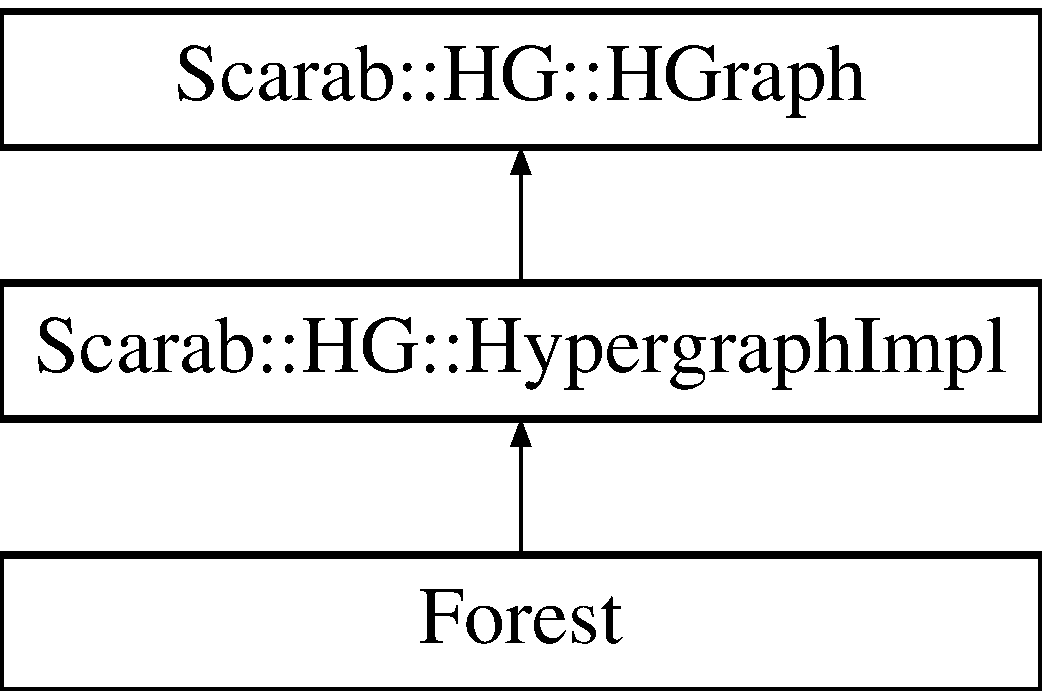
\includegraphics[height=3cm]{classForest}
\end{center}
\end{figure}
\subsection*{Public Member Functions}
\begin{DoxyCompactItemize}
\item 
void \hyperlink{classForest_a621a1a65d0f877bb33b15c79f9e24c4d}{print} () const 
\item 
\hypertarget{classForest_a4cc0cf94c18913eadd0b36f3dcf68cef}{
void {\bfseries append\_\-end\_\-nodes} ()}
\label{classForest_a4cc0cf94c18913eadd0b36f3dcf68cef}

\end{DoxyCompactItemize}
\subsection*{Static Public Member Functions}
\begin{DoxyCompactItemize}
\item 
\hypertarget{classForest_a1b9ddc0e03c1ccfcc73987fe9378fa84}{
static \hyperlink{classForest}{Forest} {\bfseries from\_\-file} (const char $\ast$file\_\-name)}
\label{classForest_a1b9ddc0e03c1ccfcc73987fe9378fa84}

\end{DoxyCompactItemize}
\subsection*{Protected Member Functions}
\begin{DoxyCompactItemize}
\item 
\hypertarget{classForest_ab40070ea9e3885d252fb7848c11f27ef}{
\hyperlink{classScarab_1_1HG_1_1Hypernode}{Scarab::HG::Hypernode} $\ast$ {\bfseries make\_\-node} (const Hypergraph\_\-Node \&node, wvector $\ast$features)}
\label{classForest_ab40070ea9e3885d252fb7848c11f27ef}

\end{DoxyCompactItemize}


\subsection{Member Function Documentation}
\hypertarget{classForest_a621a1a65d0f877bb33b15c79f9e24c4d}{
\index{Forest@{Forest}!print@{print}}
\index{print@{print}!Forest@{Forest}}
\subsubsection[{print}]{\setlength{\rightskip}{0pt plus 5cm}void Forest::print () const\hspace{0.3cm}{\ttfamily  \mbox{[}virtual\mbox{]}}}}
\label{classForest_a621a1a65d0f877bb33b15c79f9e24c4d}
Display the hypergraph for debugging. 

Implements \hyperlink{classScarab_1_1HG_1_1HGraph_ab5aa11c932b28864b56f28e0babbc1c1}{Scarab::HG::HGraph}.



The documentation for this class was generated from the following files:\begin{DoxyCompactItemize}
\item 
transforest/Forest.h\item 
transforest/Forest.cpp\end{DoxyCompactItemize}

\hypertarget{classForestLattice}{
\section{ForestLattice Class Reference}
\label{classForestLattice}\index{ForestLattice@{ForestLattice}}
}
\subsection*{Public Member Functions}
\begin{DoxyCompactItemize}
\item 
\hypertarget{classForestLattice_ad14bc799ac36b716c292f410e1609462}{
string {\bfseries get\_\-word} (int word\_\-num) const }
\label{classForestLattice_ad14bc799ac36b716c292f410e1609462}

\item 
\hypertarget{classForestLattice_a8303ce943210d4a62132f1e4054b7191}{
const \hyperlink{classScarab_1_1Graph_1_1Graph}{Graph} \& {\bfseries get\_\-graph} () const }
\label{classForestLattice_a8303ce943210d4a62132f1e4054b7191}

\item 
\hypertarget{classForestLattice_a744558d8489b4428c44275f0966d587e}{
const \hyperlink{classScarab_1_1Graph_1_1Graphnode}{Graphnode} \& {\bfseries node} (int i) const }
\label{classForestLattice_a744558d8489b4428c44275f0966d587e}

\item 
\hypertarget{classForestLattice_a8afba92a7fb437a93db30b2336ad3824}{
bool {\bfseries is\_\-phrase\_\-node} (int n) const }
\label{classForestLattice_a8afba92a7fb437a93db30b2336ad3824}

\item 
\hypertarget{classForestLattice_a9d82493dff97186334923b582999f63c}{
bool {\bfseries is\_\-word} (int w) const }
\label{classForestLattice_a9d82493dff97186334923b582999f63c}

\item 
\hypertarget{classForestLattice_a9ecaabd3e59148b28b3fad096806f9e9}{
{\bfseries ForestLattice} (const \hyperlink{classlattice_1_1Lattice}{Lattice} \&lattice)}
\label{classForestLattice_a9ecaabd3e59148b28b3fad096806f9e9}

\item 
\hypertarget{classForestLattice_a981af70e7207ece0e3454251b64fb6fa}{
int {\bfseries get\_\-edge} (int n1, int edge\_\-num) const }
\label{classForestLattice_a981af70e7207ece0e3454251b64fb6fa}

\item 
\hypertarget{classForestLattice_a142184cf6e8d4275923774edbca97f5d}{
int {\bfseries num\_\-edges} (int n) const }
\label{classForestLattice_a142184cf6e8d4275923774edbca97f5d}

\item 
\hypertarget{classForestLattice_a3921d0378a94ef040246dc87e60df1c7}{
int {\bfseries lookup\_\-word} (int w) const }
\label{classForestLattice_a3921d0378a94ef040246dc87e60df1c7}

\item 
\hypertarget{classForestLattice_a92e37fd15cd36ae5c9d0e3fe309d876e}{
int {\bfseries get\_\-edge\_\-label} (int n1, int n2) const }
\label{classForestLattice_a92e37fd15cd36ae5c9d0e3fe309d876e}

\item 
\hypertarget{classForestLattice_a2474198bedc98ef2e3c8a02ebae14f00}{
\hyperlink{structBigram}{Bigram} {\bfseries get\_\-nodes\_\-by\_\-labels} (int orig\_\-id) const }
\label{classForestLattice_a2474198bedc98ef2e3c8a02ebae14f00}

\item 
\hypertarget{classForestLattice_a6fe3508e7fd7d62b44c423dcc113881b}{
int {\bfseries num\_\-first\_\-words} (int n) const }
\label{classForestLattice_a6fe3508e7fd7d62b44c423dcc113881b}

\item 
\hypertarget{classForestLattice_ae6c29306adee71cca87bb2dc2c1047df}{
int {\bfseries num\_\-last\_\-words} (int n) const }
\label{classForestLattice_ae6c29306adee71cca87bb2dc2c1047df}

\item 
\hypertarget{classForestLattice_a7fcb5b75caf3d4e17b782849fc847ec9}{
int {\bfseries num\_\-last\_\-bigrams} (int n) const }
\label{classForestLattice_a7fcb5b75caf3d4e17b782849fc847ec9}

\item 
\hypertarget{classForestLattice_a3b8e0f2d304ad0d9b10d9efb79d7905c}{
int {\bfseries first\_\-words} (int n, int i) const }
\label{classForestLattice_a3b8e0f2d304ad0d9b10d9efb79d7905c}

\item 
\hypertarget{classForestLattice_a9af5d9ea84e0638599d13c5f78868d92}{
int {\bfseries last\_\-words} (int n, int i) const }
\label{classForestLattice_a9af5d9ea84e0638599d13c5f78868d92}

\item 
\hypertarget{classForestLattice_a3332ad66005be68e6ac38d7daa40bb9d}{
\hyperlink{structBigram}{Bigram} {\bfseries last\_\-bigrams} (int n, int i) const }
\label{classForestLattice_a3332ad66005be68e6ac38d7daa40bb9d}

\item 
\hypertarget{classForestLattice_a4da765944fa6d5892786ca592ef8c859}{
int {\bfseries get\_\-same} (int w) const }
\label{classForestLattice_a4da765944fa6d5892786ca592ef8c859}

\item 
\hypertarget{classForestLattice_a01fa72075f1de8421dd21e15540ce5c0}{
int {\bfseries get\_\-hypergraph\_\-node\_\-from\_\-word} (int w) const }
\label{classForestLattice_a01fa72075f1de8421dd21e15540ce5c0}

\item 
\hypertarget{classForestLattice_a226887bedd13a3f3dc5cbe91242bd17a}{
int {\bfseries get\_\-word\_\-from\_\-hypergraph\_\-node} (int n) const }
\label{classForestLattice_a226887bedd13a3f3dc5cbe91242bd17a}

\item 
\hypertarget{classForestLattice_a8f474062475f4d272a8d8b676cdd0118}{
void {\bfseries make\_\-proper\_\-graph} (const \hyperlink{classlattice_1_1Lattice}{Lattice} \&lat)}
\label{classForestLattice_a8f474062475f4d272a8d8b676cdd0118}

\end{DoxyCompactItemize}
\subsection*{Public Attributes}
\begin{DoxyCompactItemize}
\item 
\hypertarget{classForestLattice_a3c194341d2a88457604e0042534358fc}{
int {\bfseries num\_\-nodes}}
\label{classForestLattice_a3c194341d2a88457604e0042534358fc}

\item 
\hypertarget{classForestLattice_af7ac8b02750f52523a49b5b810e36601}{
int {\bfseries num\_\-word\_\-nodes}}
\label{classForestLattice_af7ac8b02750f52523a49b5b810e36601}

\item 
\hypertarget{classForestLattice_ab0e2ec92e11ab7d77e33c109f2451d7d}{
vector$<$ int $>$ {\bfseries final}}
\label{classForestLattice_ab0e2ec92e11ab7d77e33c109f2451d7d}

\item 
\hypertarget{classForestLattice_a95785401e57ddbcc516116f59391a7cd}{
int {\bfseries start}}
\label{classForestLattice_a95785401e57ddbcc516116f59391a7cd}

\item 
\hypertarget{classForestLattice_a2a0ccc16eaa3f83ae395c825c8bcf583}{
vector$<$ vector$<$ int $>$ $>$ {\bfseries original\_\-edges}}
\label{classForestLattice_a2a0ccc16eaa3f83ae395c825c8bcf583}

\item 
\hypertarget{classForestLattice_af55e45f3503fafeb79ef53d25abfc78b}{
vector$<$ vector$<$ int $>$ $>$ {\bfseries edges\_\-original}}
\label{classForestLattice_af55e45f3503fafeb79ef53d25abfc78b}

\item 
\hypertarget{classForestLattice_ac38a1f457fae9f29fab0b922dd8b5b81}{
vector$<$ vector$<$ \hyperlink{structBigram}{Bigram} $>$ $>$ {\bfseries bigrams\_\-at\_\-node}}
\label{classForestLattice_ac38a1f457fae9f29fab0b922dd8b5b81}

\item 
\hypertarget{classForestLattice_a80b60a05f3f81f4291b1989baf240cf8}{
vector$<$ string $>$ {\bfseries \_\-edge\_\-label\_\-by\_\-nodes}}
\label{classForestLattice_a80b60a05f3f81f4291b1989baf240cf8}

\end{DoxyCompactItemize}


The documentation for this class was generated from the following files:\begin{DoxyCompactItemize}
\item 
lattice/ForestLattice.h\item 
lattice/ForestLattice.cpp\end{DoxyCompactItemize}

\hypertarget{classForestNode}{
\section{ForestNode Class Reference}
\label{classForestNode}\index{ForestNode@{ForestNode}}
}
Inheritance diagram for ForestNode:\begin{figure}[H]
\begin{center}
\leavevmode
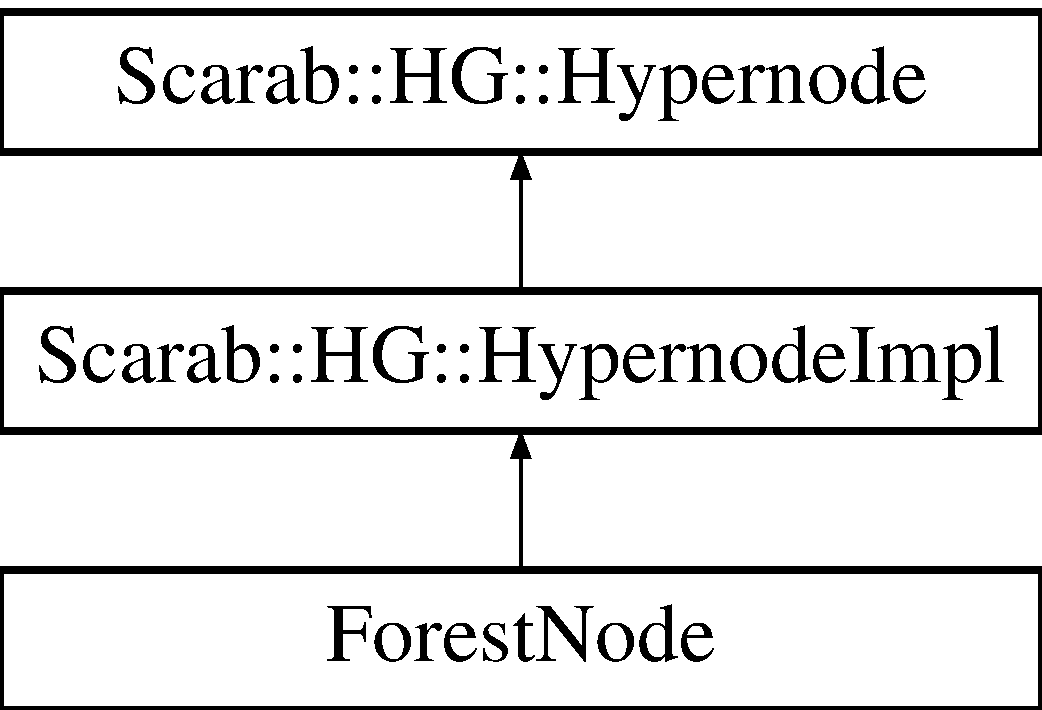
\includegraphics[height=3cm]{classForestNode}
\end{center}
\end{figure}
\subsection*{Public Member Functions}
\begin{DoxyCompactItemize}
\item 
\hypertarget{classForestNode_aeeb649eef15a82d283ae728b0a44d183}{
{\bfseries ForestNode} (const string \&label, int id, \hyperlink{classsvector}{str\_\-vector} $\ast$features, string word, bool is\_\-word)}
\label{classForestNode_aeeb649eef15a82d283ae728b0a44d183}

\item 
\hypertarget{classForestNode_ab44af8003df7af0ce93b9b904301fb92}{
bool {\bfseries is\_\-word} () const }
\label{classForestNode_ab44af8003df7af0ce93b9b904301fb92}

\item 
\hypertarget{classForestNode_a18c00f9aae93bc963358e488f2cce308}{
string {\bfseries word} () const }
\label{classForestNode_a18c00f9aae93bc963358e488f2cce308}

\end{DoxyCompactItemize}


The documentation for this class was generated from the following file:\begin{DoxyCompactItemize}
\item 
transforest/Forest.h\end{DoxyCompactItemize}

\hypertarget{classgraph_1_1Graph}{
\section{graph::Graph Class Reference}
\label{classgraph_1_1Graph}\index{graph::Graph@{graph::Graph}}
}
\subsection*{Public Types}
\begin{DoxyCompactItemize}
\item 
\hypertarget{classgraph_1_1Graph_a2a148e8d341b4850e506e4ca9a10845f}{
typedef \hyperlink{classgraph_1_1Graph__Node}{Graph\_\-Node} {\bfseries Node}}
\label{classgraph_1_1Graph_a2a148e8d341b4850e506e4ca9a10845f}

\item 
\hypertarget{classgraph_1_1Graph_ae7ba626728a03ceb51bccd5ee4ec72ca}{
typedef \hyperlink{classgraph_1_1Graph__Edge}{Graph\_\-Edge} {\bfseries Edge}}
\label{classgraph_1_1Graph_ae7ba626728a03ceb51bccd5ee4ec72ca}

\item 
\hypertarget{classgraph_1_1Graph_a2a148e8d341b4850e506e4ca9a10845f}{
typedef \hyperlink{classgraph_1_1Graph__Node}{Graph\_\-Node} {\bfseries Node}}
\label{classgraph_1_1Graph_a2a148e8d341b4850e506e4ca9a10845f}

\item 
\hypertarget{classgraph_1_1Graph_ae7ba626728a03ceb51bccd5ee4ec72ca}{
typedef \hyperlink{classgraph_1_1Graph__Edge}{Graph\_\-Edge} {\bfseries Edge}}
\label{classgraph_1_1Graph_ae7ba626728a03ceb51bccd5ee4ec72ca}

\end{DoxyCompactItemize}
\subsection*{Public Member Functions}
\begin{DoxyCompactItemize}
\item 
\hypertarget{classgraph_1_1Graph_a400fcc675124ef60cbc0d6ee0e25736c}{
{\bfseries Graph} (const \hyperlink{classgraph_1_1Graph}{Graph} \&from)}
\label{classgraph_1_1Graph_a400fcc675124ef60cbc0d6ee0e25736c}

\item 
\hypertarget{classgraph_1_1Graph_a2bb8b8cdf8632d9a9453b3f67d0eef9c}{
\hyperlink{classgraph_1_1Graph}{Graph} \& {\bfseries operator=} (const \hyperlink{classgraph_1_1Graph}{Graph} \&from)}
\label{classgraph_1_1Graph_a2bb8b8cdf8632d9a9453b3f67d0eef9c}

\item 
\hypertarget{classgraph_1_1Graph_a4944a9b85ffdbecf91ec2454f915b411}{
const ::google::protobuf::UnknownFieldSet \& {\bfseries unknown\_\-fields} () const }
\label{classgraph_1_1Graph_a4944a9b85ffdbecf91ec2454f915b411}

\item 
\hypertarget{classgraph_1_1Graph_a93081ad4e0af2767c6f57004f5f59dc2}{
inline::google::protobuf::UnknownFieldSet $\ast$ {\bfseries mutable\_\-unknown\_\-fields} ()}
\label{classgraph_1_1Graph_a93081ad4e0af2767c6f57004f5f59dc2}

\item 
\hypertarget{classgraph_1_1Graph_a8e3853558c7080802e9362e869206156}{
void {\bfseries Swap} (\hyperlink{classgraph_1_1Graph}{Graph} $\ast$other)}
\label{classgraph_1_1Graph_a8e3853558c7080802e9362e869206156}

\item 
\hypertarget{classgraph_1_1Graph_a812a4848569ca342a12b6b7a824b4118}{
\hyperlink{classgraph_1_1Graph}{Graph} $\ast$ {\bfseries New} () const }
\label{classgraph_1_1Graph_a812a4848569ca342a12b6b7a824b4118}

\item 
\hypertarget{classgraph_1_1Graph_ad8df9792d5748b48235e04e64abf84fd}{
void {\bfseries CopyFrom} (const ::google::protobuf::Message \&from)}
\label{classgraph_1_1Graph_ad8df9792d5748b48235e04e64abf84fd}

\item 
\hypertarget{classgraph_1_1Graph_ab52f15c185ebf734246297add1064b4a}{
void {\bfseries MergeFrom} (const ::google::protobuf::Message \&from)}
\label{classgraph_1_1Graph_ab52f15c185ebf734246297add1064b4a}

\item 
\hypertarget{classgraph_1_1Graph_adea321f8fe4c18ea4d2364c8b8dd54df}{
void {\bfseries CopyFrom} (const \hyperlink{classgraph_1_1Graph}{Graph} \&from)}
\label{classgraph_1_1Graph_adea321f8fe4c18ea4d2364c8b8dd54df}

\item 
\hypertarget{classgraph_1_1Graph_a918dc2343415dd9b7d0deb2c307bfb9d}{
void {\bfseries MergeFrom} (const \hyperlink{classgraph_1_1Graph}{Graph} \&from)}
\label{classgraph_1_1Graph_a918dc2343415dd9b7d0deb2c307bfb9d}

\item 
\hypertarget{classgraph_1_1Graph_a13680e6719e42aa3ebedfeb61ff06014}{
void {\bfseries Clear} ()}
\label{classgraph_1_1Graph_a13680e6719e42aa3ebedfeb61ff06014}

\item 
\hypertarget{classgraph_1_1Graph_ac91ebe6fc014af3707afd28a01bf30cc}{
bool {\bfseries IsInitialized} () const }
\label{classgraph_1_1Graph_ac91ebe6fc014af3707afd28a01bf30cc}

\item 
\hypertarget{classgraph_1_1Graph_ada721f70b6221bd45c0619de513bc138}{
int {\bfseries ByteSize} () const }
\label{classgraph_1_1Graph_ada721f70b6221bd45c0619de513bc138}

\item 
\hypertarget{classgraph_1_1Graph_a3a08a0c8418c6317a890296c25f71b9e}{
bool {\bfseries MergePartialFromCodedStream} (::google::protobuf::io::CodedInputStream $\ast$input)}
\label{classgraph_1_1Graph_a3a08a0c8418c6317a890296c25f71b9e}

\item 
\hypertarget{classgraph_1_1Graph_a69559b8d11a32f5ebe89a0c86b936ed6}{
void {\bfseries SerializeWithCachedSizes} (::google::protobuf::io::CodedOutputStream $\ast$output) const }
\label{classgraph_1_1Graph_a69559b8d11a32f5ebe89a0c86b936ed6}

\item 
\hypertarget{classgraph_1_1Graph_add26e27feb424b498dc6e7c54250886b}{
::google::protobuf::uint8 $\ast$ {\bfseries SerializeWithCachedSizesToArray} (::google::protobuf::uint8 $\ast$output) const }
\label{classgraph_1_1Graph_add26e27feb424b498dc6e7c54250886b}

\item 
\hypertarget{classgraph_1_1Graph_a2a609292df58baec63cb473317334301}{
int {\bfseries GetCachedSize} () const }
\label{classgraph_1_1Graph_a2a609292df58baec63cb473317334301}

\item 
\hypertarget{classgraph_1_1Graph_aeafa7e8b0429a852055f80767941cb38}{
::google::protobuf::Metadata {\bfseries GetMetadata} () const }
\label{classgraph_1_1Graph_aeafa7e8b0429a852055f80767941cb38}

\item 
\hypertarget{classgraph_1_1Graph_a8a43e784467fb4eda053810d73725508}{
bool {\bfseries has\_\-label} () const }
\label{classgraph_1_1Graph_a8a43e784467fb4eda053810d73725508}

\item 
\hypertarget{classgraph_1_1Graph_ae493d41f9b434145be083cbc2044c1d9}{
void {\bfseries clear\_\-label} ()}
\label{classgraph_1_1Graph_ae493d41f9b434145be083cbc2044c1d9}

\item 
\hypertarget{classgraph_1_1Graph_a7063c43da1905648d2948ce1c13d38ff}{
const ::std::string \& {\bfseries label} () const }
\label{classgraph_1_1Graph_a7063c43da1905648d2948ce1c13d38ff}

\item 
\hypertarget{classgraph_1_1Graph_ab04d4c18c9ab77ee27d5e66b92624bdd}{
void {\bfseries set\_\-label} (const ::std::string \&value)}
\label{classgraph_1_1Graph_ab04d4c18c9ab77ee27d5e66b92624bdd}

\item 
\hypertarget{classgraph_1_1Graph_a2e33bd3438f862850c7f2fad8bb3e544}{
void {\bfseries set\_\-label} (const char $\ast$value)}
\label{classgraph_1_1Graph_a2e33bd3438f862850c7f2fad8bb3e544}

\item 
\hypertarget{classgraph_1_1Graph_a829bbd790ed76b6b1729d4c719b413d7}{
void {\bfseries set\_\-label} (const char $\ast$value, size\_\-t size)}
\label{classgraph_1_1Graph_a829bbd790ed76b6b1729d4c719b413d7}

\item 
\hypertarget{classgraph_1_1Graph_ab3b46393b1918c6608320f57d9486f12}{
inline::std::string $\ast$ {\bfseries mutable\_\-label} ()}
\label{classgraph_1_1Graph_ab3b46393b1918c6608320f57d9486f12}

\item 
\hypertarget{classgraph_1_1Graph_a95233ad394bd217ae7b49bb4498e48f3}{
inline::std::string $\ast$ {\bfseries release\_\-label} ()}
\label{classgraph_1_1Graph_a95233ad394bd217ae7b49bb4498e48f3}

\item 
\hypertarget{classgraph_1_1Graph_a005baadb25b7b9611082a1c3f285cdfa}{
int {\bfseries node\_\-size} () const }
\label{classgraph_1_1Graph_a005baadb25b7b9611082a1c3f285cdfa}

\item 
\hypertarget{classgraph_1_1Graph_ad4899b84d05fc768fa335047725eaf24}{
void {\bfseries clear\_\-node} ()}
\label{classgraph_1_1Graph_ad4899b84d05fc768fa335047725eaf24}

\item 
\hypertarget{classgraph_1_1Graph_a16c29597fce7e931ed6fa7ff051a722e}{
const ::\hyperlink{classgraph_1_1Graph__Node}{graph::Graph\_\-Node} \& {\bfseries node} (int index) const }
\label{classgraph_1_1Graph_a16c29597fce7e931ed6fa7ff051a722e}

\item 
\hypertarget{classgraph_1_1Graph_a8c2e072edc54bb1450c7d9753e52e99e}{
inline::graph::Graph\_\-Node $\ast$ {\bfseries mutable\_\-node} (int index)}
\label{classgraph_1_1Graph_a8c2e072edc54bb1450c7d9753e52e99e}

\item 
\hypertarget{classgraph_1_1Graph_a853cde9df8f6492ca9b949c0e82f8eff}{
inline::graph::Graph\_\-Node $\ast$ {\bfseries add\_\-node} ()}
\label{classgraph_1_1Graph_a853cde9df8f6492ca9b949c0e82f8eff}

\item 
\hypertarget{classgraph_1_1Graph_a2bd47191520de5c1dc375cea07f61330}{
const ::google::protobuf::RepeatedPtrField$<$ ::\hyperlink{classgraph_1_1Graph__Node}{graph::Graph\_\-Node} $>$ \& {\bfseries node} () const }
\label{classgraph_1_1Graph_a2bd47191520de5c1dc375cea07f61330}

\item 
\hypertarget{classgraph_1_1Graph_a2a98be1966ff5f910c8746ffc563a1a8}{
inline::google::protobuf::RepeatedPtrField$<$ ::\hyperlink{classgraph_1_1Graph__Node}{graph::Graph\_\-Node} $>$ $\ast$ {\bfseries mutable\_\-node} ()}
\label{classgraph_1_1Graph_a2a98be1966ff5f910c8746ffc563a1a8}

\item 
\hypertarget{classgraph_1_1Graph_a400fcc675124ef60cbc0d6ee0e25736c}{
{\bfseries Graph} (const \hyperlink{classgraph_1_1Graph}{Graph} \&from)}
\label{classgraph_1_1Graph_a400fcc675124ef60cbc0d6ee0e25736c}

\item 
\hypertarget{classgraph_1_1Graph_a2bb8b8cdf8632d9a9453b3f67d0eef9c}{
\hyperlink{classgraph_1_1Graph}{Graph} \& {\bfseries operator=} (const \hyperlink{classgraph_1_1Graph}{Graph} \&from)}
\label{classgraph_1_1Graph_a2bb8b8cdf8632d9a9453b3f67d0eef9c}

\item 
\hypertarget{classgraph_1_1Graph_a4944a9b85ffdbecf91ec2454f915b411}{
const ::google::protobuf::UnknownFieldSet \& {\bfseries unknown\_\-fields} () const }
\label{classgraph_1_1Graph_a4944a9b85ffdbecf91ec2454f915b411}

\item 
\hypertarget{classgraph_1_1Graph_a93081ad4e0af2767c6f57004f5f59dc2}{
inline::google::protobuf::UnknownFieldSet $\ast$ {\bfseries mutable\_\-unknown\_\-fields} ()}
\label{classgraph_1_1Graph_a93081ad4e0af2767c6f57004f5f59dc2}

\item 
\hypertarget{classgraph_1_1Graph_a8e3853558c7080802e9362e869206156}{
void {\bfseries Swap} (\hyperlink{classgraph_1_1Graph}{Graph} $\ast$other)}
\label{classgraph_1_1Graph_a8e3853558c7080802e9362e869206156}

\item 
\hypertarget{classgraph_1_1Graph_a812a4848569ca342a12b6b7a824b4118}{
\hyperlink{classgraph_1_1Graph}{Graph} $\ast$ {\bfseries New} () const }
\label{classgraph_1_1Graph_a812a4848569ca342a12b6b7a824b4118}

\item 
\hypertarget{classgraph_1_1Graph_ad8df9792d5748b48235e04e64abf84fd}{
void {\bfseries CopyFrom} (const ::google::protobuf::Message \&from)}
\label{classgraph_1_1Graph_ad8df9792d5748b48235e04e64abf84fd}

\item 
\hypertarget{classgraph_1_1Graph_ab52f15c185ebf734246297add1064b4a}{
void {\bfseries MergeFrom} (const ::google::protobuf::Message \&from)}
\label{classgraph_1_1Graph_ab52f15c185ebf734246297add1064b4a}

\item 
\hypertarget{classgraph_1_1Graph_adea321f8fe4c18ea4d2364c8b8dd54df}{
void {\bfseries CopyFrom} (const \hyperlink{classgraph_1_1Graph}{Graph} \&from)}
\label{classgraph_1_1Graph_adea321f8fe4c18ea4d2364c8b8dd54df}

\item 
\hypertarget{classgraph_1_1Graph_a918dc2343415dd9b7d0deb2c307bfb9d}{
void {\bfseries MergeFrom} (const \hyperlink{classgraph_1_1Graph}{Graph} \&from)}
\label{classgraph_1_1Graph_a918dc2343415dd9b7d0deb2c307bfb9d}

\item 
\hypertarget{classgraph_1_1Graph_a13680e6719e42aa3ebedfeb61ff06014}{
void {\bfseries Clear} ()}
\label{classgraph_1_1Graph_a13680e6719e42aa3ebedfeb61ff06014}

\item 
\hypertarget{classgraph_1_1Graph_ac91ebe6fc014af3707afd28a01bf30cc}{
bool {\bfseries IsInitialized} () const }
\label{classgraph_1_1Graph_ac91ebe6fc014af3707afd28a01bf30cc}

\item 
\hypertarget{classgraph_1_1Graph_ada721f70b6221bd45c0619de513bc138}{
int {\bfseries ByteSize} () const }
\label{classgraph_1_1Graph_ada721f70b6221bd45c0619de513bc138}

\item 
\hypertarget{classgraph_1_1Graph_a3a08a0c8418c6317a890296c25f71b9e}{
bool {\bfseries MergePartialFromCodedStream} (::google::protobuf::io::CodedInputStream $\ast$input)}
\label{classgraph_1_1Graph_a3a08a0c8418c6317a890296c25f71b9e}

\item 
\hypertarget{classgraph_1_1Graph_a69559b8d11a32f5ebe89a0c86b936ed6}{
void {\bfseries SerializeWithCachedSizes} (::google::protobuf::io::CodedOutputStream $\ast$output) const }
\label{classgraph_1_1Graph_a69559b8d11a32f5ebe89a0c86b936ed6}

\item 
\hypertarget{classgraph_1_1Graph_add26e27feb424b498dc6e7c54250886b}{
::google::protobuf::uint8 $\ast$ {\bfseries SerializeWithCachedSizesToArray} (::google::protobuf::uint8 $\ast$output) const }
\label{classgraph_1_1Graph_add26e27feb424b498dc6e7c54250886b}

\item 
\hypertarget{classgraph_1_1Graph_a2a609292df58baec63cb473317334301}{
int {\bfseries GetCachedSize} () const }
\label{classgraph_1_1Graph_a2a609292df58baec63cb473317334301}

\item 
\hypertarget{classgraph_1_1Graph_aeafa7e8b0429a852055f80767941cb38}{
::google::protobuf::Metadata {\bfseries GetMetadata} () const }
\label{classgraph_1_1Graph_aeafa7e8b0429a852055f80767941cb38}

\item 
\hypertarget{classgraph_1_1Graph_a8a43e784467fb4eda053810d73725508}{
bool {\bfseries has\_\-label} () const }
\label{classgraph_1_1Graph_a8a43e784467fb4eda053810d73725508}

\item 
\hypertarget{classgraph_1_1Graph_ae493d41f9b434145be083cbc2044c1d9}{
void {\bfseries clear\_\-label} ()}
\label{classgraph_1_1Graph_ae493d41f9b434145be083cbc2044c1d9}

\item 
\hypertarget{classgraph_1_1Graph_aa6079fefaedc329a72194ed083c37413}{
const ::std::string \& {\bfseries label} () const }
\label{classgraph_1_1Graph_aa6079fefaedc329a72194ed083c37413}

\item 
\hypertarget{classgraph_1_1Graph_ab04d4c18c9ab77ee27d5e66b92624bdd}{
void {\bfseries set\_\-label} (const ::std::string \&value)}
\label{classgraph_1_1Graph_ab04d4c18c9ab77ee27d5e66b92624bdd}

\item 
\hypertarget{classgraph_1_1Graph_a2e33bd3438f862850c7f2fad8bb3e544}{
void {\bfseries set\_\-label} (const char $\ast$value)}
\label{classgraph_1_1Graph_a2e33bd3438f862850c7f2fad8bb3e544}

\item 
\hypertarget{classgraph_1_1Graph_a829bbd790ed76b6b1729d4c719b413d7}{
void {\bfseries set\_\-label} (const char $\ast$value, size\_\-t size)}
\label{classgraph_1_1Graph_a829bbd790ed76b6b1729d4c719b413d7}

\item 
\hypertarget{classgraph_1_1Graph_abcd3b4981aab3985879a10d16e296cfc}{
inline::std::string $\ast$ {\bfseries mutable\_\-label} ()}
\label{classgraph_1_1Graph_abcd3b4981aab3985879a10d16e296cfc}

\item 
\hypertarget{classgraph_1_1Graph_a95eb83261e9a9f59cb20b6b850c3561c}{
inline::std::string $\ast$ {\bfseries release\_\-label} ()}
\label{classgraph_1_1Graph_a95eb83261e9a9f59cb20b6b850c3561c}

\item 
\hypertarget{classgraph_1_1Graph_a005baadb25b7b9611082a1c3f285cdfa}{
int {\bfseries node\_\-size} () const }
\label{classgraph_1_1Graph_a005baadb25b7b9611082a1c3f285cdfa}

\item 
\hypertarget{classgraph_1_1Graph_ad4899b84d05fc768fa335047725eaf24}{
void {\bfseries clear\_\-node} ()}
\label{classgraph_1_1Graph_ad4899b84d05fc768fa335047725eaf24}

\item 
\hypertarget{classgraph_1_1Graph_a0d740c76c632f0670da81e6b4535d169}{
const ::\hyperlink{classgraph_1_1Graph__Node}{graph::Graph\_\-Node} \& {\bfseries node} (int index) const }
\label{classgraph_1_1Graph_a0d740c76c632f0670da81e6b4535d169}

\item 
\hypertarget{classgraph_1_1Graph_aeae06c451a4508a381f20a80322ea341}{
inline::graph::Graph\_\-Node $\ast$ {\bfseries mutable\_\-node} (int index)}
\label{classgraph_1_1Graph_aeae06c451a4508a381f20a80322ea341}

\item 
\hypertarget{classgraph_1_1Graph_a3c2452c8ed3a663cbfb9bd76acb67dc1}{
inline::graph::Graph\_\-Node $\ast$ {\bfseries add\_\-node} ()}
\label{classgraph_1_1Graph_a3c2452c8ed3a663cbfb9bd76acb67dc1}

\item 
\hypertarget{classgraph_1_1Graph_a603d1f721a181ae75db8e79e42aa86e0}{
const ::google::protobuf::RepeatedPtrField$<$ ::\hyperlink{classgraph_1_1Graph__Node}{graph::Graph\_\-Node} $>$ \& {\bfseries node} () const }
\label{classgraph_1_1Graph_a603d1f721a181ae75db8e79e42aa86e0}

\item 
\hypertarget{classgraph_1_1Graph_a54b5cfd7fe26ff67c3d8da6acd69e9b7}{
inline::google::protobuf::RepeatedPtrField$<$ ::\hyperlink{classgraph_1_1Graph__Node}{graph::Graph\_\-Node} $>$ $\ast$ {\bfseries mutable\_\-node} ()}
\label{classgraph_1_1Graph_a54b5cfd7fe26ff67c3d8da6acd69e9b7}

\end{DoxyCompactItemize}
\subsection*{Static Public Member Functions}
\begin{DoxyCompactItemize}
\item 
\hypertarget{classgraph_1_1Graph_a49c810d7ea8428dc769f56d61a24e052}{
static const ::google::protobuf::Descriptor $\ast$ {\bfseries descriptor} ()}
\label{classgraph_1_1Graph_a49c810d7ea8428dc769f56d61a24e052}

\item 
\hypertarget{classgraph_1_1Graph_a034b07f25ab695cb26a0bd5b307d72e4}{
static const \hyperlink{classgraph_1_1Graph}{Graph} \& {\bfseries default\_\-instance} ()}
\label{classgraph_1_1Graph_a034b07f25ab695cb26a0bd5b307d72e4}

\item 
\hypertarget{classgraph_1_1Graph_a49c810d7ea8428dc769f56d61a24e052}{
static const ::google::protobuf::Descriptor $\ast$ {\bfseries descriptor} ()}
\label{classgraph_1_1Graph_a49c810d7ea8428dc769f56d61a24e052}

\item 
\hypertarget{classgraph_1_1Graph_a034b07f25ab695cb26a0bd5b307d72e4}{
static const \hyperlink{classgraph_1_1Graph}{Graph} \& {\bfseries default\_\-instance} ()}
\label{classgraph_1_1Graph_a034b07f25ab695cb26a0bd5b307d72e4}

\end{DoxyCompactItemize}
\subsection*{Static Public Attributes}
\begin{DoxyCompactItemize}
\item 
\hypertarget{classgraph_1_1Graph_a2969c2c72eb20aaca51ff8e34e607914}{
static const int {\bfseries kLabelFieldNumber} = 5}
\label{classgraph_1_1Graph_a2969c2c72eb20aaca51ff8e34e607914}

\item 
\hypertarget{classgraph_1_1Graph_a3784b95d1729d17dcaf95adbda08c119}{
static const int {\bfseries kNodeFieldNumber} = 6}
\label{classgraph_1_1Graph_a3784b95d1729d17dcaf95adbda08c119}

\end{DoxyCompactItemize}
\subsection*{Friends}
\begin{DoxyCompactItemize}
\item 
\hypertarget{classgraph_1_1Graph_a3216c708da10839178deebea43d6f0be}{
void {\bfseries protobuf\_\-AddDesc\_\-graph\_\-2eproto} ()}
\label{classgraph_1_1Graph_a3216c708da10839178deebea43d6f0be}

\item 
\hypertarget{classgraph_1_1Graph_a4c9d7eb8f9e30e490c8bcae70e629de5}{
void {\bfseries protobuf\_\-AssignDesc\_\-graph\_\-2eproto} ()}
\label{classgraph_1_1Graph_a4c9d7eb8f9e30e490c8bcae70e629de5}

\item 
\hypertarget{classgraph_1_1Graph_aac10332314561225d8ac09b797223f3d}{
void {\bfseries protobuf\_\-ShutdownFile\_\-graph\_\-2eproto} ()}
\label{classgraph_1_1Graph_aac10332314561225d8ac09b797223f3d}

\item 
\hypertarget{classgraph_1_1Graph_a3216c708da10839178deebea43d6f0be}{
void {\bfseries protobuf\_\-AddDesc\_\-graph\_\-2eproto} ()}
\label{classgraph_1_1Graph_a3216c708da10839178deebea43d6f0be}

\item 
\hypertarget{classgraph_1_1Graph_a4c9d7eb8f9e30e490c8bcae70e629de5}{
void {\bfseries protobuf\_\-AssignDesc\_\-graph\_\-2eproto} ()}
\label{classgraph_1_1Graph_a4c9d7eb8f9e30e490c8bcae70e629de5}

\item 
\hypertarget{classgraph_1_1Graph_aac10332314561225d8ac09b797223f3d}{
void {\bfseries protobuf\_\-ShutdownFile\_\-graph\_\-2eproto} ()}
\label{classgraph_1_1Graph_aac10332314561225d8ac09b797223f3d}

\end{DoxyCompactItemize}


The documentation for this class was generated from the following files:\begin{DoxyCompactItemize}
\item 
interfaces/graph/gen-\/cpp/graph.pb.h\item 
interfaces/graph/gen-\/py/graph.pb.h\end{DoxyCompactItemize}

\hypertarget{classScarab_1_1Graph_1_1Graph}{
\section{Scarab::Graph::Graph Class Reference}
\label{classScarab_1_1Graph_1_1Graph}\index{Scarab::Graph::Graph@{Scarab::Graph::Graph}}
}
\subsection*{Public Member Functions}
\begin{DoxyCompactItemize}
\item 
\hypertarget{classScarab_1_1Graph_1_1Graph_ac753f9750341458516e06fb1437a1258}{
{\bfseries Graph} (const Nodes \&nodes, const Edges \&edges)}
\label{classScarab_1_1Graph_1_1Graph_ac753f9750341458516e06fb1437a1258}

\item 
uint \hyperlink{classScarab_1_1Graph_1_1Graph_afdfbdd8e5427a646707ceb22ca15d2e2}{num\_\-edges} () const 
\item 
\hypertarget{classScarab_1_1Graph_1_1Graph_ac35877b52ec1f625ff452a4073026b26}{
uint {\bfseries num\_\-nodes} () const }
\label{classScarab_1_1Graph_1_1Graph_ac35877b52ec1f625ff452a4073026b26}

\item 
\hypertarget{classScarab_1_1Graph_1_1Graph_a8d0c6189ef1569626348a30e908870e4}{
const Nodes \& {\bfseries nodes} () const }
\label{classScarab_1_1Graph_1_1Graph_a8d0c6189ef1569626348a30e908870e4}

\item 
\hypertarget{classScarab_1_1Graph_1_1Graph_a19a63be838e64b57e46cba029e273162}{
const Edges \& {\bfseries edges} () const }
\label{classScarab_1_1Graph_1_1Graph_a19a63be838e64b57e46cba029e273162}

\item 
\hypertarget{classScarab_1_1Graph_1_1Graph_af226b4907b00e178a8f7bd6e972e42d2}{
const \hyperlink{classScarab_1_1Graph_1_1Graphnode}{Graphnode} \& {\bfseries node} (uint i) const }
\label{classScarab_1_1Graph_1_1Graph_af226b4907b00e178a8f7bd6e972e42d2}

\end{DoxyCompactItemize}


\subsection{Member Function Documentation}
\hypertarget{classScarab_1_1Graph_1_1Graph_afdfbdd8e5427a646707ceb22ca15d2e2}{
\index{Scarab::Graph::Graph@{Scarab::Graph::Graph}!num\_\-edges@{num\_\-edges}}
\index{num\_\-edges@{num\_\-edges}!Scarab::Graph::Graph@{Scarab::Graph::Graph}}
\subsubsection[{num\_\-edges}]{\setlength{\rightskip}{0pt plus 5cm}uint Scarab::Graph::Graph::num\_\-edges () const\hspace{0.3cm}{\ttfamily  \mbox{[}inline\mbox{]}}}}
\label{classScarab_1_1Graph_1_1Graph_afdfbdd8e5427a646707ceb22ca15d2e2}
Display the graph for debugging. 

The documentation for this class was generated from the following file:\begin{DoxyCompactItemize}
\item 
graph/Graph.h\end{DoxyCompactItemize}

\hypertarget{classgraph_1_1Graph__Edge}{
\section{graph::Graph\_\-Edge Class Reference}
\label{classgraph_1_1Graph__Edge}\index{graph::Graph\_\-Edge@{graph::Graph\_\-Edge}}
}
\subsection*{Public Member Functions}
\begin{DoxyCompactItemize}
\item 
\hypertarget{classgraph_1_1Graph__Edge_a1b8cdd9aa0720a4b78149954fb109810}{
{\bfseries Graph\_\-Edge} (const \hyperlink{classgraph_1_1Graph__Edge}{Graph\_\-Edge} \&from)}
\label{classgraph_1_1Graph__Edge_a1b8cdd9aa0720a4b78149954fb109810}

\item 
\hypertarget{classgraph_1_1Graph__Edge_a271827f73c4c315e95210cccb000e8f1}{
\hyperlink{classgraph_1_1Graph__Edge}{Graph\_\-Edge} \& {\bfseries operator=} (const \hyperlink{classgraph_1_1Graph__Edge}{Graph\_\-Edge} \&from)}
\label{classgraph_1_1Graph__Edge_a271827f73c4c315e95210cccb000e8f1}

\item 
\hypertarget{classgraph_1_1Graph__Edge_ad3839379afb5e8a8965bbfa48e6ab52c}{
const ::google::protobuf::UnknownFieldSet \& {\bfseries unknown\_\-fields} () const }
\label{classgraph_1_1Graph__Edge_ad3839379afb5e8a8965bbfa48e6ab52c}

\item 
\hypertarget{classgraph_1_1Graph__Edge_ab23e809a21f594cc319a0d1f781fa384}{
inline::google::protobuf::UnknownFieldSet $\ast$ {\bfseries mutable\_\-unknown\_\-fields} ()}
\label{classgraph_1_1Graph__Edge_ab23e809a21f594cc319a0d1f781fa384}

\item 
\hypertarget{classgraph_1_1Graph__Edge_aaaf2710e8754faf829d2966551176aac}{
void {\bfseries Swap} (\hyperlink{classgraph_1_1Graph__Edge}{Graph\_\-Edge} $\ast$other)}
\label{classgraph_1_1Graph__Edge_aaaf2710e8754faf829d2966551176aac}

\item 
\hypertarget{classgraph_1_1Graph__Edge_a724cb0402b0736d438d0e99c04e83548}{
\hyperlink{classgraph_1_1Graph__Edge}{Graph\_\-Edge} $\ast$ {\bfseries New} () const }
\label{classgraph_1_1Graph__Edge_a724cb0402b0736d438d0e99c04e83548}

\item 
\hypertarget{classgraph_1_1Graph__Edge_ae610eaa471b68f5c8effe5bd28b5cf8c}{
void {\bfseries CopyFrom} (const ::google::protobuf::Message \&from)}
\label{classgraph_1_1Graph__Edge_ae610eaa471b68f5c8effe5bd28b5cf8c}

\item 
\hypertarget{classgraph_1_1Graph__Edge_a21df881962677b6db77cd0fc6fdb8086}{
void {\bfseries MergeFrom} (const ::google::protobuf::Message \&from)}
\label{classgraph_1_1Graph__Edge_a21df881962677b6db77cd0fc6fdb8086}

\item 
\hypertarget{classgraph_1_1Graph__Edge_a70c9bb7cbaad6263cf5b67a61315daaf}{
void {\bfseries CopyFrom} (const \hyperlink{classgraph_1_1Graph__Edge}{Graph\_\-Edge} \&from)}
\label{classgraph_1_1Graph__Edge_a70c9bb7cbaad6263cf5b67a61315daaf}

\item 
\hypertarget{classgraph_1_1Graph__Edge_a9c6886542c53a31f42ae5ea9afa826c2}{
void {\bfseries MergeFrom} (const \hyperlink{classgraph_1_1Graph__Edge}{Graph\_\-Edge} \&from)}
\label{classgraph_1_1Graph__Edge_a9c6886542c53a31f42ae5ea9afa826c2}

\item 
\hypertarget{classgraph_1_1Graph__Edge_a2bbcc59dbf4e00c8f3007fa89b5470a9}{
void {\bfseries Clear} ()}
\label{classgraph_1_1Graph__Edge_a2bbcc59dbf4e00c8f3007fa89b5470a9}

\item 
\hypertarget{classgraph_1_1Graph__Edge_a9d94dfbfe951e8e834ccf837901c51dd}{
bool {\bfseries IsInitialized} () const }
\label{classgraph_1_1Graph__Edge_a9d94dfbfe951e8e834ccf837901c51dd}

\item 
\hypertarget{classgraph_1_1Graph__Edge_a76a24bfd2a4d0f0f79df2014bb4d184d}{
int {\bfseries ByteSize} () const }
\label{classgraph_1_1Graph__Edge_a76a24bfd2a4d0f0f79df2014bb4d184d}

\item 
\hypertarget{classgraph_1_1Graph__Edge_aed892b9333d734dde9a338fafa4ea497}{
bool {\bfseries MergePartialFromCodedStream} (::google::protobuf::io::CodedInputStream $\ast$input)}
\label{classgraph_1_1Graph__Edge_aed892b9333d734dde9a338fafa4ea497}

\item 
\hypertarget{classgraph_1_1Graph__Edge_a0f0582860901bfb055dda63c7193e7e3}{
void {\bfseries SerializeWithCachedSizes} (::google::protobuf::io::CodedOutputStream $\ast$output) const }
\label{classgraph_1_1Graph__Edge_a0f0582860901bfb055dda63c7193e7e3}

\item 
\hypertarget{classgraph_1_1Graph__Edge_ac4f89968c18ff0151c7536e843d5760a}{
::google::protobuf::uint8 $\ast$ {\bfseries SerializeWithCachedSizesToArray} (::google::protobuf::uint8 $\ast$output) const }
\label{classgraph_1_1Graph__Edge_ac4f89968c18ff0151c7536e843d5760a}

\item 
\hypertarget{classgraph_1_1Graph__Edge_aeb53e0cc707fcb6d3e329541b293d919}{
int {\bfseries GetCachedSize} () const }
\label{classgraph_1_1Graph__Edge_aeb53e0cc707fcb6d3e329541b293d919}

\item 
\hypertarget{classgraph_1_1Graph__Edge_a9f96696a40f9f41012fd4bb7883b031d}{
::google::protobuf::Metadata {\bfseries GetMetadata} () const }
\label{classgraph_1_1Graph__Edge_a9f96696a40f9f41012fd4bb7883b031d}

\item 
\hypertarget{classgraph_1_1Graph__Edge_a0190e8f222646d5e304732d71d28b310}{
bool {\bfseries has\_\-id} () const }
\label{classgraph_1_1Graph__Edge_a0190e8f222646d5e304732d71d28b310}

\item 
\hypertarget{classgraph_1_1Graph__Edge_ab04135cf552e93eceb7abb38077140ba}{
void {\bfseries clear\_\-id} ()}
\label{classgraph_1_1Graph__Edge_ab04135cf552e93eceb7abb38077140ba}

\item 
\hypertarget{classgraph_1_1Graph__Edge_a4e73f471d038367947b20597ace18391}{
inline::google::protobuf::int32 {\bfseries id} () const }
\label{classgraph_1_1Graph__Edge_a4e73f471d038367947b20597ace18391}

\item 
\hypertarget{classgraph_1_1Graph__Edge_a9d0281649c61d01a499e9d4a0dcc35bb}{
void {\bfseries set\_\-id} (::google::protobuf::int32 value)}
\label{classgraph_1_1Graph__Edge_a9d0281649c61d01a499e9d4a0dcc35bb}

\item 
\hypertarget{classgraph_1_1Graph__Edge_a002aa4e1a3cbb1d3ae04f811ad5499f5}{
bool {\bfseries has\_\-label} () const }
\label{classgraph_1_1Graph__Edge_a002aa4e1a3cbb1d3ae04f811ad5499f5}

\item 
\hypertarget{classgraph_1_1Graph__Edge_a88236828360ba4677de28dcd11a0c892}{
void {\bfseries clear\_\-label} ()}
\label{classgraph_1_1Graph__Edge_a88236828360ba4677de28dcd11a0c892}

\item 
\hypertarget{classgraph_1_1Graph__Edge_a30909562219911929f8af6402de78abc}{
const ::std::string \& {\bfseries label} () const }
\label{classgraph_1_1Graph__Edge_a30909562219911929f8af6402de78abc}

\item 
\hypertarget{classgraph_1_1Graph__Edge_ae0b7d66524cdb3c239a4658c6ebe49ed}{
void {\bfseries set\_\-label} (const ::std::string \&value)}
\label{classgraph_1_1Graph__Edge_ae0b7d66524cdb3c239a4658c6ebe49ed}

\item 
\hypertarget{classgraph_1_1Graph__Edge_a5e28d3ae41aa291b904c97f8086e6599}{
void {\bfseries set\_\-label} (const char $\ast$value)}
\label{classgraph_1_1Graph__Edge_a5e28d3ae41aa291b904c97f8086e6599}

\item 
\hypertarget{classgraph_1_1Graph__Edge_ab5e92ddc8c7a81e0e7689cb86dac75ce}{
void {\bfseries set\_\-label} (const char $\ast$value, size\_\-t size)}
\label{classgraph_1_1Graph__Edge_ab5e92ddc8c7a81e0e7689cb86dac75ce}

\item 
\hypertarget{classgraph_1_1Graph__Edge_a35d039789edd950847ab757c9b0ef07a}{
inline::std::string $\ast$ {\bfseries mutable\_\-label} ()}
\label{classgraph_1_1Graph__Edge_a35d039789edd950847ab757c9b0ef07a}

\item 
\hypertarget{classgraph_1_1Graph__Edge_ab85ac3ad8bb604fa41030a547b2763ec}{
inline::std::string $\ast$ {\bfseries release\_\-label} ()}
\label{classgraph_1_1Graph__Edge_ab85ac3ad8bb604fa41030a547b2763ec}

\item 
\hypertarget{classgraph_1_1Graph__Edge_af80c945f9d34527de487207bc9553776}{
bool {\bfseries has\_\-to\_\-node} () const }
\label{classgraph_1_1Graph__Edge_af80c945f9d34527de487207bc9553776}

\item 
\hypertarget{classgraph_1_1Graph__Edge_a10c4766efe37b9ebf33d94e58f5d34d1}{
void {\bfseries clear\_\-to\_\-node} ()}
\label{classgraph_1_1Graph__Edge_a10c4766efe37b9ebf33d94e58f5d34d1}

\item 
\hypertarget{classgraph_1_1Graph__Edge_aedbaf240950d5029ab5c13a1b09c19e1}{
inline::google::protobuf::int32 {\bfseries to\_\-node} () const }
\label{classgraph_1_1Graph__Edge_aedbaf240950d5029ab5c13a1b09c19e1}

\item 
\hypertarget{classgraph_1_1Graph__Edge_a61b1469e26d71c6b2673a6a3da5a057f}{
void {\bfseries set\_\-to\_\-node} (::google::protobuf::int32 value)}
\label{classgraph_1_1Graph__Edge_a61b1469e26d71c6b2673a6a3da5a057f}

\item 
\hypertarget{classgraph_1_1Graph__Edge_a1b8cdd9aa0720a4b78149954fb109810}{
{\bfseries Graph\_\-Edge} (const \hyperlink{classgraph_1_1Graph__Edge}{Graph\_\-Edge} \&from)}
\label{classgraph_1_1Graph__Edge_a1b8cdd9aa0720a4b78149954fb109810}

\item 
\hypertarget{classgraph_1_1Graph__Edge_a271827f73c4c315e95210cccb000e8f1}{
\hyperlink{classgraph_1_1Graph__Edge}{Graph\_\-Edge} \& {\bfseries operator=} (const \hyperlink{classgraph_1_1Graph__Edge}{Graph\_\-Edge} \&from)}
\label{classgraph_1_1Graph__Edge_a271827f73c4c315e95210cccb000e8f1}

\item 
\hypertarget{classgraph_1_1Graph__Edge_ad3839379afb5e8a8965bbfa48e6ab52c}{
const ::google::protobuf::UnknownFieldSet \& {\bfseries unknown\_\-fields} () const }
\label{classgraph_1_1Graph__Edge_ad3839379afb5e8a8965bbfa48e6ab52c}

\item 
\hypertarget{classgraph_1_1Graph__Edge_ab23e809a21f594cc319a0d1f781fa384}{
inline::google::protobuf::UnknownFieldSet $\ast$ {\bfseries mutable\_\-unknown\_\-fields} ()}
\label{classgraph_1_1Graph__Edge_ab23e809a21f594cc319a0d1f781fa384}

\item 
\hypertarget{classgraph_1_1Graph__Edge_aaaf2710e8754faf829d2966551176aac}{
void {\bfseries Swap} (\hyperlink{classgraph_1_1Graph__Edge}{Graph\_\-Edge} $\ast$other)}
\label{classgraph_1_1Graph__Edge_aaaf2710e8754faf829d2966551176aac}

\item 
\hypertarget{classgraph_1_1Graph__Edge_a0758753878823f19c37d391d965a4fc3}{
\hyperlink{classgraph_1_1Graph__Edge}{Graph\_\-Edge} $\ast$ {\bfseries New} () const }
\label{classgraph_1_1Graph__Edge_a0758753878823f19c37d391d965a4fc3}

\item 
\hypertarget{classgraph_1_1Graph__Edge_ae610eaa471b68f5c8effe5bd28b5cf8c}{
void {\bfseries CopyFrom} (const ::google::protobuf::Message \&from)}
\label{classgraph_1_1Graph__Edge_ae610eaa471b68f5c8effe5bd28b5cf8c}

\item 
\hypertarget{classgraph_1_1Graph__Edge_a21df881962677b6db77cd0fc6fdb8086}{
void {\bfseries MergeFrom} (const ::google::protobuf::Message \&from)}
\label{classgraph_1_1Graph__Edge_a21df881962677b6db77cd0fc6fdb8086}

\item 
\hypertarget{classgraph_1_1Graph__Edge_a70c9bb7cbaad6263cf5b67a61315daaf}{
void {\bfseries CopyFrom} (const \hyperlink{classgraph_1_1Graph__Edge}{Graph\_\-Edge} \&from)}
\label{classgraph_1_1Graph__Edge_a70c9bb7cbaad6263cf5b67a61315daaf}

\item 
\hypertarget{classgraph_1_1Graph__Edge_a9c6886542c53a31f42ae5ea9afa826c2}{
void {\bfseries MergeFrom} (const \hyperlink{classgraph_1_1Graph__Edge}{Graph\_\-Edge} \&from)}
\label{classgraph_1_1Graph__Edge_a9c6886542c53a31f42ae5ea9afa826c2}

\item 
\hypertarget{classgraph_1_1Graph__Edge_a2bbcc59dbf4e00c8f3007fa89b5470a9}{
void {\bfseries Clear} ()}
\label{classgraph_1_1Graph__Edge_a2bbcc59dbf4e00c8f3007fa89b5470a9}

\item 
\hypertarget{classgraph_1_1Graph__Edge_a9d94dfbfe951e8e834ccf837901c51dd}{
bool {\bfseries IsInitialized} () const }
\label{classgraph_1_1Graph__Edge_a9d94dfbfe951e8e834ccf837901c51dd}

\item 
\hypertarget{classgraph_1_1Graph__Edge_a76a24bfd2a4d0f0f79df2014bb4d184d}{
int {\bfseries ByteSize} () const }
\label{classgraph_1_1Graph__Edge_a76a24bfd2a4d0f0f79df2014bb4d184d}

\item 
\hypertarget{classgraph_1_1Graph__Edge_aed892b9333d734dde9a338fafa4ea497}{
bool {\bfseries MergePartialFromCodedStream} (::google::protobuf::io::CodedInputStream $\ast$input)}
\label{classgraph_1_1Graph__Edge_aed892b9333d734dde9a338fafa4ea497}

\item 
\hypertarget{classgraph_1_1Graph__Edge_a0f0582860901bfb055dda63c7193e7e3}{
void {\bfseries SerializeWithCachedSizes} (::google::protobuf::io::CodedOutputStream $\ast$output) const }
\label{classgraph_1_1Graph__Edge_a0f0582860901bfb055dda63c7193e7e3}

\item 
\hypertarget{classgraph_1_1Graph__Edge_a864e056928fefb48751ba22f97064d3f}{
::google::protobuf::uint8 $\ast$ {\bfseries SerializeWithCachedSizesToArray} (::google::protobuf::uint8 $\ast$output) const }
\label{classgraph_1_1Graph__Edge_a864e056928fefb48751ba22f97064d3f}

\item 
\hypertarget{classgraph_1_1Graph__Edge_aeb53e0cc707fcb6d3e329541b293d919}{
int {\bfseries GetCachedSize} () const }
\label{classgraph_1_1Graph__Edge_aeb53e0cc707fcb6d3e329541b293d919}

\item 
\hypertarget{classgraph_1_1Graph__Edge_a323a96197c86ad300ddf7f63cda021b7}{
::google::protobuf::Metadata {\bfseries GetMetadata} () const }
\label{classgraph_1_1Graph__Edge_a323a96197c86ad300ddf7f63cda021b7}

\item 
\hypertarget{classgraph_1_1Graph__Edge_a0190e8f222646d5e304732d71d28b310}{
bool {\bfseries has\_\-id} () const }
\label{classgraph_1_1Graph__Edge_a0190e8f222646d5e304732d71d28b310}

\item 
\hypertarget{classgraph_1_1Graph__Edge_ab04135cf552e93eceb7abb38077140ba}{
void {\bfseries clear\_\-id} ()}
\label{classgraph_1_1Graph__Edge_ab04135cf552e93eceb7abb38077140ba}

\item 
\hypertarget{classgraph_1_1Graph__Edge_a3cb43575a65d2d2b4b3f10f2f368a6e5}{
inline::google::protobuf::int32 {\bfseries id} () const }
\label{classgraph_1_1Graph__Edge_a3cb43575a65d2d2b4b3f10f2f368a6e5}

\item 
\hypertarget{classgraph_1_1Graph__Edge_a9d0281649c61d01a499e9d4a0dcc35bb}{
void {\bfseries set\_\-id} (::google::protobuf::int32 value)}
\label{classgraph_1_1Graph__Edge_a9d0281649c61d01a499e9d4a0dcc35bb}

\item 
\hypertarget{classgraph_1_1Graph__Edge_a002aa4e1a3cbb1d3ae04f811ad5499f5}{
bool {\bfseries has\_\-label} () const }
\label{classgraph_1_1Graph__Edge_a002aa4e1a3cbb1d3ae04f811ad5499f5}

\item 
\hypertarget{classgraph_1_1Graph__Edge_a88236828360ba4677de28dcd11a0c892}{
void {\bfseries clear\_\-label} ()}
\label{classgraph_1_1Graph__Edge_a88236828360ba4677de28dcd11a0c892}

\item 
\hypertarget{classgraph_1_1Graph__Edge_a1c2c35183332758b8519875e9a6d9bad}{
const ::std::string \& {\bfseries label} () const }
\label{classgraph_1_1Graph__Edge_a1c2c35183332758b8519875e9a6d9bad}

\item 
\hypertarget{classgraph_1_1Graph__Edge_ae0b7d66524cdb3c239a4658c6ebe49ed}{
void {\bfseries set\_\-label} (const ::std::string \&value)}
\label{classgraph_1_1Graph__Edge_ae0b7d66524cdb3c239a4658c6ebe49ed}

\item 
\hypertarget{classgraph_1_1Graph__Edge_a5e28d3ae41aa291b904c97f8086e6599}{
void {\bfseries set\_\-label} (const char $\ast$value)}
\label{classgraph_1_1Graph__Edge_a5e28d3ae41aa291b904c97f8086e6599}

\item 
\hypertarget{classgraph_1_1Graph__Edge_ab5e92ddc8c7a81e0e7689cb86dac75ce}{
void {\bfseries set\_\-label} (const char $\ast$value, size\_\-t size)}
\label{classgraph_1_1Graph__Edge_ab5e92ddc8c7a81e0e7689cb86dac75ce}

\item 
\hypertarget{classgraph_1_1Graph__Edge_a79e66e701e4f30c74db839df05649037}{
inline::std::string $\ast$ {\bfseries mutable\_\-label} ()}
\label{classgraph_1_1Graph__Edge_a79e66e701e4f30c74db839df05649037}

\item 
\hypertarget{classgraph_1_1Graph__Edge_a932083f61d90db20cf811adaf02503fd}{
inline::std::string $\ast$ {\bfseries release\_\-label} ()}
\label{classgraph_1_1Graph__Edge_a932083f61d90db20cf811adaf02503fd}

\item 
\hypertarget{classgraph_1_1Graph__Edge_af80c945f9d34527de487207bc9553776}{
bool {\bfseries has\_\-to\_\-node} () const }
\label{classgraph_1_1Graph__Edge_af80c945f9d34527de487207bc9553776}

\item 
\hypertarget{classgraph_1_1Graph__Edge_a10c4766efe37b9ebf33d94e58f5d34d1}{
void {\bfseries clear\_\-to\_\-node} ()}
\label{classgraph_1_1Graph__Edge_a10c4766efe37b9ebf33d94e58f5d34d1}

\item 
\hypertarget{classgraph_1_1Graph__Edge_ae2c9acb9f4e76e8228947b44eba690f9}{
inline::google::protobuf::int32 {\bfseries to\_\-node} () const }
\label{classgraph_1_1Graph__Edge_ae2c9acb9f4e76e8228947b44eba690f9}

\item 
\hypertarget{classgraph_1_1Graph__Edge_a61b1469e26d71c6b2673a6a3da5a057f}{
void {\bfseries set\_\-to\_\-node} (::google::protobuf::int32 value)}
\label{classgraph_1_1Graph__Edge_a61b1469e26d71c6b2673a6a3da5a057f}

\end{DoxyCompactItemize}
\subsection*{Static Public Member Functions}
\begin{DoxyCompactItemize}
\item 
\hypertarget{classgraph_1_1Graph__Edge_ab32bdc6778944caff5d93501c0d8d202}{
static const ::google::protobuf::Descriptor $\ast$ {\bfseries descriptor} ()}
\label{classgraph_1_1Graph__Edge_ab32bdc6778944caff5d93501c0d8d202}

\item 
\hypertarget{classgraph_1_1Graph__Edge_aec4df3118608258ce28ce41b217abebf}{
static const \hyperlink{classgraph_1_1Graph__Edge}{Graph\_\-Edge} \& {\bfseries default\_\-instance} ()}
\label{classgraph_1_1Graph__Edge_aec4df3118608258ce28ce41b217abebf}

\item 
\hypertarget{classgraph_1_1Graph__Edge_a3123a39b6f9e2e2fac9035944ce1d589}{
static const ::google::protobuf::Descriptor $\ast$ {\bfseries descriptor} ()}
\label{classgraph_1_1Graph__Edge_a3123a39b6f9e2e2fac9035944ce1d589}

\item 
\hypertarget{classgraph_1_1Graph__Edge_a14f42efa9ab2cf6559077dd0fdd05f34}{
static const \hyperlink{classgraph_1_1Graph__Edge}{Graph\_\-Edge} \& {\bfseries default\_\-instance} ()}
\label{classgraph_1_1Graph__Edge_a14f42efa9ab2cf6559077dd0fdd05f34}

\end{DoxyCompactItemize}
\subsection*{Static Public Attributes}
\begin{DoxyCompactItemize}
\item 
\hypertarget{classgraph_1_1Graph__Edge_a72855929893523a2ab0b28c29e6de404}{
static const int {\bfseries kIdFieldNumber} = 1}
\label{classgraph_1_1Graph__Edge_a72855929893523a2ab0b28c29e6de404}

\item 
\hypertarget{classgraph_1_1Graph__Edge_a6a3f7f24e4560ba96be0534f45781197}{
static const int {\bfseries kLabelFieldNumber} = 2}
\label{classgraph_1_1Graph__Edge_a6a3f7f24e4560ba96be0534f45781197}

\item 
\hypertarget{classgraph_1_1Graph__Edge_a15d36a93bd22e587021c53b7b3e16e84}{
static const int {\bfseries kToNodeFieldNumber} = 3}
\label{classgraph_1_1Graph__Edge_a15d36a93bd22e587021c53b7b3e16e84}

\end{DoxyCompactItemize}
\subsection*{Friends}
\begin{DoxyCompactItemize}
\item 
\hypertarget{classgraph_1_1Graph__Edge_a3216c708da10839178deebea43d6f0be}{
void {\bfseries protobuf\_\-AddDesc\_\-graph\_\-2eproto} ()}
\label{classgraph_1_1Graph__Edge_a3216c708da10839178deebea43d6f0be}

\item 
\hypertarget{classgraph_1_1Graph__Edge_a4c9d7eb8f9e30e490c8bcae70e629de5}{
void {\bfseries protobuf\_\-AssignDesc\_\-graph\_\-2eproto} ()}
\label{classgraph_1_1Graph__Edge_a4c9d7eb8f9e30e490c8bcae70e629de5}

\item 
\hypertarget{classgraph_1_1Graph__Edge_aac10332314561225d8ac09b797223f3d}{
void {\bfseries protobuf\_\-ShutdownFile\_\-graph\_\-2eproto} ()}
\label{classgraph_1_1Graph__Edge_aac10332314561225d8ac09b797223f3d}

\item 
\hypertarget{classgraph_1_1Graph__Edge_a3216c708da10839178deebea43d6f0be}{
void {\bfseries protobuf\_\-AddDesc\_\-graph\_\-2eproto} ()}
\label{classgraph_1_1Graph__Edge_a3216c708da10839178deebea43d6f0be}

\item 
\hypertarget{classgraph_1_1Graph__Edge_a4c9d7eb8f9e30e490c8bcae70e629de5}{
void {\bfseries protobuf\_\-AssignDesc\_\-graph\_\-2eproto} ()}
\label{classgraph_1_1Graph__Edge_a4c9d7eb8f9e30e490c8bcae70e629de5}

\item 
\hypertarget{classgraph_1_1Graph__Edge_aac10332314561225d8ac09b797223f3d}{
void {\bfseries protobuf\_\-ShutdownFile\_\-graph\_\-2eproto} ()}
\label{classgraph_1_1Graph__Edge_aac10332314561225d8ac09b797223f3d}

\end{DoxyCompactItemize}


The documentation for this class was generated from the following files:\begin{DoxyCompactItemize}
\item 
interfaces/graph/gen-\/cpp/graph.pb.h\item 
interfaces/graph/gen-\/py/graph.pb.h\item 
interfaces/graph/gen-\/cpp/graph.pb.cc\item 
interfaces/graph/gen-\/py/graph.pb.cc\end{DoxyCompactItemize}

\hypertarget{classgraph_1_1Graph__Node}{
\section{graph::Graph\_\-Node Class Reference}
\label{classgraph_1_1Graph__Node}\index{graph::Graph\_\-Node@{graph::Graph\_\-Node}}
}
\subsection*{Public Member Functions}
\begin{DoxyCompactItemize}
\item 
\hypertarget{classgraph_1_1Graph__Node_a3e14dbbb1960cdceb42a22f191851a6b}{
{\bfseries Graph\_\-Node} (const \hyperlink{classgraph_1_1Graph__Node}{Graph\_\-Node} \&from)}
\label{classgraph_1_1Graph__Node_a3e14dbbb1960cdceb42a22f191851a6b}

\item 
\hypertarget{classgraph_1_1Graph__Node_a1b117f5f955e29ec6e990e50cc2026e0}{
\hyperlink{classgraph_1_1Graph__Node}{Graph\_\-Node} \& {\bfseries operator=} (const \hyperlink{classgraph_1_1Graph__Node}{Graph\_\-Node} \&from)}
\label{classgraph_1_1Graph__Node_a1b117f5f955e29ec6e990e50cc2026e0}

\item 
\hypertarget{classgraph_1_1Graph__Node_a1292a0d7a11d6709ee0a3bffd699ddc6}{
const ::google::protobuf::UnknownFieldSet \& {\bfseries unknown\_\-fields} () const }
\label{classgraph_1_1Graph__Node_a1292a0d7a11d6709ee0a3bffd699ddc6}

\item 
\hypertarget{classgraph_1_1Graph__Node_a458590dbf61732e966b050e46a5b9ee0}{
inline::google::protobuf::UnknownFieldSet $\ast$ {\bfseries mutable\_\-unknown\_\-fields} ()}
\label{classgraph_1_1Graph__Node_a458590dbf61732e966b050e46a5b9ee0}

\item 
\hypertarget{classgraph_1_1Graph__Node_a7161b02ad669bb3c0eba53b5231467d9}{
void {\bfseries Swap} (\hyperlink{classgraph_1_1Graph__Node}{Graph\_\-Node} $\ast$other)}
\label{classgraph_1_1Graph__Node_a7161b02ad669bb3c0eba53b5231467d9}

\item 
\hypertarget{classgraph_1_1Graph__Node_a29347d8834678e64e08cddccc5c0a3dc}{
\hyperlink{classgraph_1_1Graph__Node}{Graph\_\-Node} $\ast$ {\bfseries New} () const }
\label{classgraph_1_1Graph__Node_a29347d8834678e64e08cddccc5c0a3dc}

\item 
\hypertarget{classgraph_1_1Graph__Node_a5f3eca853b1a6ab6d72b95fc63edc476}{
void {\bfseries CopyFrom} (const ::google::protobuf::Message \&from)}
\label{classgraph_1_1Graph__Node_a5f3eca853b1a6ab6d72b95fc63edc476}

\item 
\hypertarget{classgraph_1_1Graph__Node_a4c182ee38bc9ad649a9ae67f9ba5ae18}{
void {\bfseries MergeFrom} (const ::google::protobuf::Message \&from)}
\label{classgraph_1_1Graph__Node_a4c182ee38bc9ad649a9ae67f9ba5ae18}

\item 
\hypertarget{classgraph_1_1Graph__Node_ab2ba680d4220f5c206b77aa8dafd5816}{
void {\bfseries CopyFrom} (const \hyperlink{classgraph_1_1Graph__Node}{Graph\_\-Node} \&from)}
\label{classgraph_1_1Graph__Node_ab2ba680d4220f5c206b77aa8dafd5816}

\item 
\hypertarget{classgraph_1_1Graph__Node_a979ddc18e4e1238cf396311c6622ef43}{
void {\bfseries MergeFrom} (const \hyperlink{classgraph_1_1Graph__Node}{Graph\_\-Node} \&from)}
\label{classgraph_1_1Graph__Node_a979ddc18e4e1238cf396311c6622ef43}

\item 
\hypertarget{classgraph_1_1Graph__Node_a4bddb506c7141091ad3989769a535604}{
void {\bfseries Clear} ()}
\label{classgraph_1_1Graph__Node_a4bddb506c7141091ad3989769a535604}

\item 
\hypertarget{classgraph_1_1Graph__Node_a60da720d929b8e8d5aefd410466c3871}{
bool {\bfseries IsInitialized} () const }
\label{classgraph_1_1Graph__Node_a60da720d929b8e8d5aefd410466c3871}

\item 
\hypertarget{classgraph_1_1Graph__Node_ab25a1fde48166c7639063b5750b9887b}{
int {\bfseries ByteSize} () const }
\label{classgraph_1_1Graph__Node_ab25a1fde48166c7639063b5750b9887b}

\item 
\hypertarget{classgraph_1_1Graph__Node_a3d4ce335c0bc53aa858c0e7a87a257e7}{
bool {\bfseries MergePartialFromCodedStream} (::google::protobuf::io::CodedInputStream $\ast$input)}
\label{classgraph_1_1Graph__Node_a3d4ce335c0bc53aa858c0e7a87a257e7}

\item 
\hypertarget{classgraph_1_1Graph__Node_ac36ab307cedb19991696faea055dc7e1}{
void {\bfseries SerializeWithCachedSizes} (::google::protobuf::io::CodedOutputStream $\ast$output) const }
\label{classgraph_1_1Graph__Node_ac36ab307cedb19991696faea055dc7e1}

\item 
\hypertarget{classgraph_1_1Graph__Node_ab38db8ff30a7ec5d376f07cb5e7a329a}{
::google::protobuf::uint8 $\ast$ {\bfseries SerializeWithCachedSizesToArray} (::google::protobuf::uint8 $\ast$output) const }
\label{classgraph_1_1Graph__Node_ab38db8ff30a7ec5d376f07cb5e7a329a}

\item 
\hypertarget{classgraph_1_1Graph__Node_a6a61a74708a5efef4c4103e70d9f2345}{
int {\bfseries GetCachedSize} () const }
\label{classgraph_1_1Graph__Node_a6a61a74708a5efef4c4103e70d9f2345}

\item 
\hypertarget{classgraph_1_1Graph__Node_adb976064f2dc0f91f69766e8477e2715}{
::google::protobuf::Metadata {\bfseries GetMetadata} () const }
\label{classgraph_1_1Graph__Node_adb976064f2dc0f91f69766e8477e2715}

\item 
\hypertarget{classgraph_1_1Graph__Node_a13671ab38b485b1ca616604da78e0342}{
bool {\bfseries has\_\-id} () const }
\label{classgraph_1_1Graph__Node_a13671ab38b485b1ca616604da78e0342}

\item 
\hypertarget{classgraph_1_1Graph__Node_a410170becd9a924a4e3d68bc344f8091}{
void {\bfseries clear\_\-id} ()}
\label{classgraph_1_1Graph__Node_a410170becd9a924a4e3d68bc344f8091}

\item 
\hypertarget{classgraph_1_1Graph__Node_a5576e6256d0ace782444007de0ad5c33}{
inline::google::protobuf::int32 {\bfseries id} () const }
\label{classgraph_1_1Graph__Node_a5576e6256d0ace782444007de0ad5c33}

\item 
\hypertarget{classgraph_1_1Graph__Node_a3855150c0788095990243586449ad2bd}{
void {\bfseries set\_\-id} (::google::protobuf::int32 value)}
\label{classgraph_1_1Graph__Node_a3855150c0788095990243586449ad2bd}

\item 
\hypertarget{classgraph_1_1Graph__Node_a9a4e1f3901310d63d085c1320c611732}{
bool {\bfseries has\_\-label} () const }
\label{classgraph_1_1Graph__Node_a9a4e1f3901310d63d085c1320c611732}

\item 
\hypertarget{classgraph_1_1Graph__Node_a45185f565e515460b8f67aa35e58b0b0}{
void {\bfseries clear\_\-label} ()}
\label{classgraph_1_1Graph__Node_a45185f565e515460b8f67aa35e58b0b0}

\item 
\hypertarget{classgraph_1_1Graph__Node_a32d2b07f0ec89ac74ae1c27d21f0920d}{
const ::std::string \& {\bfseries label} () const }
\label{classgraph_1_1Graph__Node_a32d2b07f0ec89ac74ae1c27d21f0920d}

\item 
\hypertarget{classgraph_1_1Graph__Node_ac7d3363065ac3e53045612da423e8063}{
void {\bfseries set\_\-label} (const ::std::string \&value)}
\label{classgraph_1_1Graph__Node_ac7d3363065ac3e53045612da423e8063}

\item 
\hypertarget{classgraph_1_1Graph__Node_a15d313094babc84b96727fc0f3c1d8ec}{
void {\bfseries set\_\-label} (const char $\ast$value)}
\label{classgraph_1_1Graph__Node_a15d313094babc84b96727fc0f3c1d8ec}

\item 
\hypertarget{classgraph_1_1Graph__Node_a1919f6fa3da8bfd42a347bf6600ce8b8}{
void {\bfseries set\_\-label} (const char $\ast$value, size\_\-t size)}
\label{classgraph_1_1Graph__Node_a1919f6fa3da8bfd42a347bf6600ce8b8}

\item 
\hypertarget{classgraph_1_1Graph__Node_a64ce191c10f7be3108cfe4de3734a24e}{
inline::std::string $\ast$ {\bfseries mutable\_\-label} ()}
\label{classgraph_1_1Graph__Node_a64ce191c10f7be3108cfe4de3734a24e}

\item 
\hypertarget{classgraph_1_1Graph__Node_a6182277dadee1694a4f934a62b37a0f6}{
inline::std::string $\ast$ {\bfseries release\_\-label} ()}
\label{classgraph_1_1Graph__Node_a6182277dadee1694a4f934a62b37a0f6}

\item 
\hypertarget{classgraph_1_1Graph__Node_aa33c2e20c45055a5f5c64fde8f475b12}{
int {\bfseries edge\_\-size} () const }
\label{classgraph_1_1Graph__Node_aa33c2e20c45055a5f5c64fde8f475b12}

\item 
\hypertarget{classgraph_1_1Graph__Node_a71d1bf9742cb25c8c902a1e04f9c5117}{
void {\bfseries clear\_\-edge} ()}
\label{classgraph_1_1Graph__Node_a71d1bf9742cb25c8c902a1e04f9c5117}

\item 
\hypertarget{classgraph_1_1Graph__Node_affb8668609150e1076fc749edff09ad9}{
const ::\hyperlink{classgraph_1_1Graph__Edge}{graph::Graph\_\-Edge} \& {\bfseries edge} (int index) const }
\label{classgraph_1_1Graph__Node_affb8668609150e1076fc749edff09ad9}

\item 
\hypertarget{classgraph_1_1Graph__Node_a9fa2877552b88627c05bd22d418ecd33}{
inline::graph::Graph\_\-Edge $\ast$ {\bfseries mutable\_\-edge} (int index)}
\label{classgraph_1_1Graph__Node_a9fa2877552b88627c05bd22d418ecd33}

\item 
\hypertarget{classgraph_1_1Graph__Node_ac7df0608e84959110b7a40b099012416}{
inline::graph::Graph\_\-Edge $\ast$ {\bfseries add\_\-edge} ()}
\label{classgraph_1_1Graph__Node_ac7df0608e84959110b7a40b099012416}

\item 
\hypertarget{classgraph_1_1Graph__Node_a8d151fb4b6cf825838b1bcc3c9309935}{
const ::google::protobuf::RepeatedPtrField$<$ ::\hyperlink{classgraph_1_1Graph__Edge}{graph::Graph\_\-Edge} $>$ \& {\bfseries edge} () const }
\label{classgraph_1_1Graph__Node_a8d151fb4b6cf825838b1bcc3c9309935}

\item 
\hypertarget{classgraph_1_1Graph__Node_a7ee0a29b23254291137f2ff6d090fa08}{
inline::google::protobuf::RepeatedPtrField$<$ ::\hyperlink{classgraph_1_1Graph__Edge}{graph::Graph\_\-Edge} $>$ $\ast$ {\bfseries mutable\_\-edge} ()}
\label{classgraph_1_1Graph__Node_a7ee0a29b23254291137f2ff6d090fa08}

\item 
\hypertarget{classgraph_1_1Graph__Node_a3e14dbbb1960cdceb42a22f191851a6b}{
{\bfseries Graph\_\-Node} (const \hyperlink{classgraph_1_1Graph__Node}{Graph\_\-Node} \&from)}
\label{classgraph_1_1Graph__Node_a3e14dbbb1960cdceb42a22f191851a6b}

\item 
\hypertarget{classgraph_1_1Graph__Node_a1b117f5f955e29ec6e990e50cc2026e0}{
\hyperlink{classgraph_1_1Graph__Node}{Graph\_\-Node} \& {\bfseries operator=} (const \hyperlink{classgraph_1_1Graph__Node}{Graph\_\-Node} \&from)}
\label{classgraph_1_1Graph__Node_a1b117f5f955e29ec6e990e50cc2026e0}

\item 
\hypertarget{classgraph_1_1Graph__Node_a1292a0d7a11d6709ee0a3bffd699ddc6}{
const ::google::protobuf::UnknownFieldSet \& {\bfseries unknown\_\-fields} () const }
\label{classgraph_1_1Graph__Node_a1292a0d7a11d6709ee0a3bffd699ddc6}

\item 
\hypertarget{classgraph_1_1Graph__Node_a458590dbf61732e966b050e46a5b9ee0}{
inline::google::protobuf::UnknownFieldSet $\ast$ {\bfseries mutable\_\-unknown\_\-fields} ()}
\label{classgraph_1_1Graph__Node_a458590dbf61732e966b050e46a5b9ee0}

\item 
\hypertarget{classgraph_1_1Graph__Node_a7161b02ad669bb3c0eba53b5231467d9}{
void {\bfseries Swap} (\hyperlink{classgraph_1_1Graph__Node}{Graph\_\-Node} $\ast$other)}
\label{classgraph_1_1Graph__Node_a7161b02ad669bb3c0eba53b5231467d9}

\item 
\hypertarget{classgraph_1_1Graph__Node_a29347d8834678e64e08cddccc5c0a3dc}{
\hyperlink{classgraph_1_1Graph__Node}{Graph\_\-Node} $\ast$ {\bfseries New} () const }
\label{classgraph_1_1Graph__Node_a29347d8834678e64e08cddccc5c0a3dc}

\item 
\hypertarget{classgraph_1_1Graph__Node_a5f3eca853b1a6ab6d72b95fc63edc476}{
void {\bfseries CopyFrom} (const ::google::protobuf::Message \&from)}
\label{classgraph_1_1Graph__Node_a5f3eca853b1a6ab6d72b95fc63edc476}

\item 
\hypertarget{classgraph_1_1Graph__Node_a4c182ee38bc9ad649a9ae67f9ba5ae18}{
void {\bfseries MergeFrom} (const ::google::protobuf::Message \&from)}
\label{classgraph_1_1Graph__Node_a4c182ee38bc9ad649a9ae67f9ba5ae18}

\item 
\hypertarget{classgraph_1_1Graph__Node_ab2ba680d4220f5c206b77aa8dafd5816}{
void {\bfseries CopyFrom} (const \hyperlink{classgraph_1_1Graph__Node}{Graph\_\-Node} \&from)}
\label{classgraph_1_1Graph__Node_ab2ba680d4220f5c206b77aa8dafd5816}

\item 
\hypertarget{classgraph_1_1Graph__Node_a979ddc18e4e1238cf396311c6622ef43}{
void {\bfseries MergeFrom} (const \hyperlink{classgraph_1_1Graph__Node}{Graph\_\-Node} \&from)}
\label{classgraph_1_1Graph__Node_a979ddc18e4e1238cf396311c6622ef43}

\item 
\hypertarget{classgraph_1_1Graph__Node_a4bddb506c7141091ad3989769a535604}{
void {\bfseries Clear} ()}
\label{classgraph_1_1Graph__Node_a4bddb506c7141091ad3989769a535604}

\item 
\hypertarget{classgraph_1_1Graph__Node_a60da720d929b8e8d5aefd410466c3871}{
bool {\bfseries IsInitialized} () const }
\label{classgraph_1_1Graph__Node_a60da720d929b8e8d5aefd410466c3871}

\item 
\hypertarget{classgraph_1_1Graph__Node_ab25a1fde48166c7639063b5750b9887b}{
int {\bfseries ByteSize} () const }
\label{classgraph_1_1Graph__Node_ab25a1fde48166c7639063b5750b9887b}

\item 
\hypertarget{classgraph_1_1Graph__Node_a3d4ce335c0bc53aa858c0e7a87a257e7}{
bool {\bfseries MergePartialFromCodedStream} (::google::protobuf::io::CodedInputStream $\ast$input)}
\label{classgraph_1_1Graph__Node_a3d4ce335c0bc53aa858c0e7a87a257e7}

\item 
\hypertarget{classgraph_1_1Graph__Node_ac36ab307cedb19991696faea055dc7e1}{
void {\bfseries SerializeWithCachedSizes} (::google::protobuf::io::CodedOutputStream $\ast$output) const }
\label{classgraph_1_1Graph__Node_ac36ab307cedb19991696faea055dc7e1}

\item 
\hypertarget{classgraph_1_1Graph__Node_ab38db8ff30a7ec5d376f07cb5e7a329a}{
::google::protobuf::uint8 $\ast$ {\bfseries SerializeWithCachedSizesToArray} (::google::protobuf::uint8 $\ast$output) const }
\label{classgraph_1_1Graph__Node_ab38db8ff30a7ec5d376f07cb5e7a329a}

\item 
\hypertarget{classgraph_1_1Graph__Node_a6a61a74708a5efef4c4103e70d9f2345}{
int {\bfseries GetCachedSize} () const }
\label{classgraph_1_1Graph__Node_a6a61a74708a5efef4c4103e70d9f2345}

\item 
\hypertarget{classgraph_1_1Graph__Node_adb976064f2dc0f91f69766e8477e2715}{
::google::protobuf::Metadata {\bfseries GetMetadata} () const }
\label{classgraph_1_1Graph__Node_adb976064f2dc0f91f69766e8477e2715}

\item 
\hypertarget{classgraph_1_1Graph__Node_a13671ab38b485b1ca616604da78e0342}{
bool {\bfseries has\_\-id} () const }
\label{classgraph_1_1Graph__Node_a13671ab38b485b1ca616604da78e0342}

\item 
\hypertarget{classgraph_1_1Graph__Node_a410170becd9a924a4e3d68bc344f8091}{
void {\bfseries clear\_\-id} ()}
\label{classgraph_1_1Graph__Node_a410170becd9a924a4e3d68bc344f8091}

\item 
\hypertarget{classgraph_1_1Graph__Node_a3a33f43632377ce6b0709364b3122a0e}{
inline::google::protobuf::int32 {\bfseries id} () const }
\label{classgraph_1_1Graph__Node_a3a33f43632377ce6b0709364b3122a0e}

\item 
\hypertarget{classgraph_1_1Graph__Node_a3855150c0788095990243586449ad2bd}{
void {\bfseries set\_\-id} (::google::protobuf::int32 value)}
\label{classgraph_1_1Graph__Node_a3855150c0788095990243586449ad2bd}

\item 
\hypertarget{classgraph_1_1Graph__Node_a9a4e1f3901310d63d085c1320c611732}{
bool {\bfseries has\_\-label} () const }
\label{classgraph_1_1Graph__Node_a9a4e1f3901310d63d085c1320c611732}

\item 
\hypertarget{classgraph_1_1Graph__Node_a45185f565e515460b8f67aa35e58b0b0}{
void {\bfseries clear\_\-label} ()}
\label{classgraph_1_1Graph__Node_a45185f565e515460b8f67aa35e58b0b0}

\item 
\hypertarget{classgraph_1_1Graph__Node_a8fb9a4c28287a6568798ca99cf2fcd77}{
const ::std::string \& {\bfseries label} () const }
\label{classgraph_1_1Graph__Node_a8fb9a4c28287a6568798ca99cf2fcd77}

\item 
\hypertarget{classgraph_1_1Graph__Node_ac7d3363065ac3e53045612da423e8063}{
void {\bfseries set\_\-label} (const ::std::string \&value)}
\label{classgraph_1_1Graph__Node_ac7d3363065ac3e53045612da423e8063}

\item 
\hypertarget{classgraph_1_1Graph__Node_a15d313094babc84b96727fc0f3c1d8ec}{
void {\bfseries set\_\-label} (const char $\ast$value)}
\label{classgraph_1_1Graph__Node_a15d313094babc84b96727fc0f3c1d8ec}

\item 
\hypertarget{classgraph_1_1Graph__Node_a1919f6fa3da8bfd42a347bf6600ce8b8}{
void {\bfseries set\_\-label} (const char $\ast$value, size\_\-t size)}
\label{classgraph_1_1Graph__Node_a1919f6fa3da8bfd42a347bf6600ce8b8}

\item 
\hypertarget{classgraph_1_1Graph__Node_a88bb3c0873b401bc7057b829b141ee40}{
inline::std::string $\ast$ {\bfseries mutable\_\-label} ()}
\label{classgraph_1_1Graph__Node_a88bb3c0873b401bc7057b829b141ee40}

\item 
\hypertarget{classgraph_1_1Graph__Node_a44b318000f10362c94dd75f2d6dd340f}{
inline::std::string $\ast$ {\bfseries release\_\-label} ()}
\label{classgraph_1_1Graph__Node_a44b318000f10362c94dd75f2d6dd340f}

\item 
\hypertarget{classgraph_1_1Graph__Node_aa33c2e20c45055a5f5c64fde8f475b12}{
int {\bfseries edge\_\-size} () const }
\label{classgraph_1_1Graph__Node_aa33c2e20c45055a5f5c64fde8f475b12}

\item 
\hypertarget{classgraph_1_1Graph__Node_a71d1bf9742cb25c8c902a1e04f9c5117}{
void {\bfseries clear\_\-edge} ()}
\label{classgraph_1_1Graph__Node_a71d1bf9742cb25c8c902a1e04f9c5117}

\item 
\hypertarget{classgraph_1_1Graph__Node_a22a50a45912b9092b9226607a35c1224}{
const ::\hyperlink{classgraph_1_1Graph__Edge}{graph::Graph\_\-Edge} \& {\bfseries edge} (int index) const }
\label{classgraph_1_1Graph__Node_a22a50a45912b9092b9226607a35c1224}

\item 
\hypertarget{classgraph_1_1Graph__Node_ab67ca8df7129110d5e50550ada39ee48}{
inline::graph::Graph\_\-Edge $\ast$ {\bfseries mutable\_\-edge} (int index)}
\label{classgraph_1_1Graph__Node_ab67ca8df7129110d5e50550ada39ee48}

\item 
\hypertarget{classgraph_1_1Graph__Node_a1217ffa590fdd95eab7d8f9d3b464b4a}{
inline::graph::Graph\_\-Edge $\ast$ {\bfseries add\_\-edge} ()}
\label{classgraph_1_1Graph__Node_a1217ffa590fdd95eab7d8f9d3b464b4a}

\item 
\hypertarget{classgraph_1_1Graph__Node_a39199d3d605e718a856c869eed3ba256}{
const ::google::protobuf::RepeatedPtrField$<$ ::\hyperlink{classgraph_1_1Graph__Edge}{graph::Graph\_\-Edge} $>$ \& {\bfseries edge} () const }
\label{classgraph_1_1Graph__Node_a39199d3d605e718a856c869eed3ba256}

\item 
\hypertarget{classgraph_1_1Graph__Node_a3ec630a7375b6c99d6a2808a5f9e430e}{
inline::google::protobuf::RepeatedPtrField$<$ ::\hyperlink{classgraph_1_1Graph__Edge}{graph::Graph\_\-Edge} $>$ $\ast$ {\bfseries mutable\_\-edge} ()}
\label{classgraph_1_1Graph__Node_a3ec630a7375b6c99d6a2808a5f9e430e}

\end{DoxyCompactItemize}
\subsection*{Static Public Member Functions}
\begin{DoxyCompactItemize}
\item 
\hypertarget{classgraph_1_1Graph__Node_a2a1ebf9c3fc400c7d650576338e3fa97}{
static const ::google::protobuf::Descriptor $\ast$ {\bfseries descriptor} ()}
\label{classgraph_1_1Graph__Node_a2a1ebf9c3fc400c7d650576338e3fa97}

\item 
\hypertarget{classgraph_1_1Graph__Node_a9cd51eafd2aadb24dc3af6ca9fd67051}{
static const \hyperlink{classgraph_1_1Graph__Node}{Graph\_\-Node} \& {\bfseries default\_\-instance} ()}
\label{classgraph_1_1Graph__Node_a9cd51eafd2aadb24dc3af6ca9fd67051}

\item 
\hypertarget{classgraph_1_1Graph__Node_a2a1ebf9c3fc400c7d650576338e3fa97}{
static const ::google::protobuf::Descriptor $\ast$ {\bfseries descriptor} ()}
\label{classgraph_1_1Graph__Node_a2a1ebf9c3fc400c7d650576338e3fa97}

\item 
\hypertarget{classgraph_1_1Graph__Node_a9cd51eafd2aadb24dc3af6ca9fd67051}{
static const \hyperlink{classgraph_1_1Graph__Node}{Graph\_\-Node} \& {\bfseries default\_\-instance} ()}
\label{classgraph_1_1Graph__Node_a9cd51eafd2aadb24dc3af6ca9fd67051}

\end{DoxyCompactItemize}
\subsection*{Static Public Attributes}
\begin{DoxyCompactItemize}
\item 
\hypertarget{classgraph_1_1Graph__Node_a64bb5b3869f25b9090ab28bb9a36771c}{
static const int {\bfseries kIdFieldNumber} = 1}
\label{classgraph_1_1Graph__Node_a64bb5b3869f25b9090ab28bb9a36771c}

\item 
\hypertarget{classgraph_1_1Graph__Node_ad7acd0364613fb8c7705b73c4501f1a2}{
static const int {\bfseries kLabelFieldNumber} = 2}
\label{classgraph_1_1Graph__Node_ad7acd0364613fb8c7705b73c4501f1a2}

\item 
\hypertarget{classgraph_1_1Graph__Node_a4e420c8292b17a5c36c317485d324025}{
static const int {\bfseries kEdgeFieldNumber} = 3}
\label{classgraph_1_1Graph__Node_a4e420c8292b17a5c36c317485d324025}

\end{DoxyCompactItemize}
\subsection*{Friends}
\begin{DoxyCompactItemize}
\item 
\hypertarget{classgraph_1_1Graph__Node_a3216c708da10839178deebea43d6f0be}{
void {\bfseries protobuf\_\-AddDesc\_\-graph\_\-2eproto} ()}
\label{classgraph_1_1Graph__Node_a3216c708da10839178deebea43d6f0be}

\item 
\hypertarget{classgraph_1_1Graph__Node_a4c9d7eb8f9e30e490c8bcae70e629de5}{
void {\bfseries protobuf\_\-AssignDesc\_\-graph\_\-2eproto} ()}
\label{classgraph_1_1Graph__Node_a4c9d7eb8f9e30e490c8bcae70e629de5}

\item 
\hypertarget{classgraph_1_1Graph__Node_aac10332314561225d8ac09b797223f3d}{
void {\bfseries protobuf\_\-ShutdownFile\_\-graph\_\-2eproto} ()}
\label{classgraph_1_1Graph__Node_aac10332314561225d8ac09b797223f3d}

\item 
\hypertarget{classgraph_1_1Graph__Node_a3216c708da10839178deebea43d6f0be}{
void {\bfseries protobuf\_\-AddDesc\_\-graph\_\-2eproto} ()}
\label{classgraph_1_1Graph__Node_a3216c708da10839178deebea43d6f0be}

\item 
\hypertarget{classgraph_1_1Graph__Node_a4c9d7eb8f9e30e490c8bcae70e629de5}{
void {\bfseries protobuf\_\-AssignDesc\_\-graph\_\-2eproto} ()}
\label{classgraph_1_1Graph__Node_a4c9d7eb8f9e30e490c8bcae70e629de5}

\item 
\hypertarget{classgraph_1_1Graph__Node_aac10332314561225d8ac09b797223f3d}{
void {\bfseries protobuf\_\-ShutdownFile\_\-graph\_\-2eproto} ()}
\label{classgraph_1_1Graph__Node_aac10332314561225d8ac09b797223f3d}

\end{DoxyCompactItemize}


The documentation for this class was generated from the following files:\begin{DoxyCompactItemize}
\item 
interfaces/graph/gen-\/cpp/graph.pb.h\item 
interfaces/graph/gen-\/py/graph.pb.h\end{DoxyCompactItemize}

\hypertarget{classGraphDecompose}{
\section{GraphDecompose Class Reference}
\label{classGraphDecompose}\index{GraphDecompose@{GraphDecompose}}
}
\subsection*{Public Member Functions}
\begin{DoxyCompactItemize}
\item 
\hypertarget{classGraphDecompose_a671b195e2a0eff48eeefcee64d40fcb1}{
void {\bfseries decompose} (const \hyperlink{classForestLattice}{ForestLattice} $\ast$g)}
\label{classGraphDecompose_a671b195e2a0eff48eeefcee64d40fcb1}

\item 
\hypertarget{classGraphDecompose_a8e85b51d78e6bd961bbff6d121399ba7}{
bool {\bfseries path\_\-exists} (int w1, int w2) const }
\label{classGraphDecompose_a8e85b51d78e6bd961bbff6d121399ba7}

\item 
\hypertarget{classGraphDecompose_a48e47d62512330c280ed8a89bafe3e10}{
vector$<$ int $>$ $\ast$ {\bfseries get\_\-path} (int w1, int w2) const }
\label{classGraphDecompose_a48e47d62512330c280ed8a89bafe3e10}

\end{DoxyCompactItemize}
\subsection*{Public Attributes}
\begin{DoxyCompactItemize}
\item 
\hypertarget{classGraphDecompose_afbeb52935da971f4bc27f0e80ed48d33}{
vector$<$ \hyperlink{structBigram}{Bigram} $>$ {\bfseries valid\_\-bigrams}}
\label{classGraphDecompose_afbeb52935da971f4bc27f0e80ed48d33}

\item 
\hypertarget{classGraphDecompose_aca254d25cf0f2d2ad0d58a5775a297a8}{
vector$<$ vector$<$ int $>$ $>$ {\bfseries forward\_\-bigrams}}
\label{classGraphDecompose_aca254d25cf0f2d2ad0d58a5775a297a8}

\item 
\hypertarget{classGraphDecompose_a2b5c495d7725ccd63c0c3d2590ebd1e1}{
vector$<$ vector$<$ int $>$ $>$ {\bfseries backward\_\-bigrams}}
\label{classGraphDecompose_a2b5c495d7725ccd63c0c3d2590ebd1e1}

\end{DoxyCompactItemize}


The documentation for this class was generated from the following files:\begin{DoxyCompactItemize}
\item 
lattice/GraphDecompose.h\item 
lattice/GraphDecompose.cpp\end{DoxyCompactItemize}

\hypertarget{classScarab_1_1Graph_1_1Graphedge}{
\section{Scarab::Graph::Graphedge Class Reference}
\label{classScarab_1_1Graph_1_1Graphedge}\index{Scarab::Graph::Graphedge@{Scarab::Graph::Graphedge}}
}
\subsection*{Public Member Functions}
\begin{DoxyCompactItemize}
\item 
\hypertarget{classScarab_1_1Graph_1_1Graphedge_aea165d2e0b46a46180f5e684df52abdf}{
{\bfseries Graphedge} (uint id, const \hyperlink{classScarab_1_1Graph_1_1Graphnode}{Graphnode} \&from, const \hyperlink{classScarab_1_1Graph_1_1Graphnode}{Graphnode} \&to)}
\label{classScarab_1_1Graph_1_1Graphedge_aea165d2e0b46a46180f5e684df52abdf}

\item 
uint \hyperlink{classScarab_1_1Graph_1_1Graphedge_af4e2b922eb0db014aa6af45ef911e47c}{id} () const 
\item 
\hypertarget{classScarab_1_1Graph_1_1Graphedge_a10760ab9034b358f9bd4aa28c44117d5}{
\hyperlink{classScarab_1_1Graph_1_1Graphnode}{Node} {\bfseries from\_\-node} () const }
\label{classScarab_1_1Graph_1_1Graphedge_a10760ab9034b358f9bd4aa28c44117d5}

\item 
\hypertarget{classScarab_1_1Graph_1_1Graphedge_ae5b1fccfa8a11847b8be2a27690243f0}{
\hyperlink{classScarab_1_1Graph_1_1Graphnode}{Node} {\bfseries to\_\-node} () const }
\label{classScarab_1_1Graph_1_1Graphedge_ae5b1fccfa8a11847b8be2a27690243f0}

\end{DoxyCompactItemize}


\subsection{Member Function Documentation}
\hypertarget{classScarab_1_1Graph_1_1Graphedge_af4e2b922eb0db014aa6af45ef911e47c}{
\index{Scarab::Graph::Graphedge@{Scarab::Graph::Graphedge}!id@{id}}
\index{id@{id}!Scarab::Graph::Graphedge@{Scarab::Graph::Graphedge}}
\subsubsection[{id}]{\setlength{\rightskip}{0pt plus 5cm}uint Scarab::Graph::Graphedge::id () const\hspace{0.3cm}{\ttfamily  \mbox{[}inline\mbox{]}}}}
\label{classScarab_1_1Graph_1_1Graphedge_af4e2b922eb0db014aa6af45ef911e47c}
Get edge id

\begin{DoxyReturn}{Returns}
The id of this edge in a fixed hypergraph 
\end{DoxyReturn}


The documentation for this class was generated from the following file:\begin{DoxyCompactItemize}
\item 
graph/Graph.h\end{DoxyCompactItemize}

\hypertarget{classScarab_1_1Graph_1_1Graphnode}{
\section{Scarab::Graph::Graphnode Class Reference}
\label{classScarab_1_1Graph_1_1Graphnode}\index{Scarab::Graph::Graphnode@{Scarab::Graph::Graphnode}}
}
\subsection*{Public Member Functions}
\begin{DoxyCompactItemize}
\item 
\hypertarget{classScarab_1_1Graph_1_1Graphnode_adce1b3b5b83d8fca4952f244bd093b9f}{
{\bfseries Graphnode} (uint id)}
\label{classScarab_1_1Graph_1_1Graphnode_adce1b3b5b83d8fca4952f244bd093b9f}

\item 
uint \hyperlink{classScarab_1_1Graph_1_1Graphnode_a74eaaed5d31a0a2c0445f3de0859148f}{id} () const 
\item 
uint \hyperlink{classScarab_1_1Graph_1_1Graphnode_a78229cc45113d24f1373a50a13bc7be4}{num\_\-edges} () const 
\item 
\hypertarget{classScarab_1_1Graph_1_1Graphnode_a717294ebbae2d29e9f97633407dae4ce}{
uint {\bfseries num\_\-in\_\-edges} () const }
\label{classScarab_1_1Graph_1_1Graphnode_a717294ebbae2d29e9f97633407dae4ce}

\item 
const Edges \& \hyperlink{classScarab_1_1Graph_1_1Graphnode_a4ffd990052c812242cbdeeae7b0e1104}{edges} () const 
\item 
\hypertarget{classScarab_1_1Graph_1_1Graphnode_a001915a0fd7a6d4b06886f7865fc5189}{
const Edges \& {\bfseries in\_\-edges} () const }
\label{classScarab_1_1Graph_1_1Graphnode_a001915a0fd7a6d4b06886f7865fc5189}

\item 
\hypertarget{classScarab_1_1Graph_1_1Graphnode_ae37c75fd607395376ade1cda5294e2a4}{
void {\bfseries set\_\-edges} (Edges edges)}
\label{classScarab_1_1Graph_1_1Graphnode_ae37c75fd607395376ade1cda5294e2a4}

\item 
\hypertarget{classScarab_1_1Graph_1_1Graphnode_a22e722e5bcd49dcfa643304d631416dc}{
void {\bfseries add\_\-edge} (\hyperlink{classScarab_1_1Graph_1_1Graphedge}{Edge} edge)}
\label{classScarab_1_1Graph_1_1Graphnode_a22e722e5bcd49dcfa643304d631416dc}

\item 
\hypertarget{classScarab_1_1Graph_1_1Graphnode_a092b914639364b7b9168c84e3e556cea}{
void {\bfseries add\_\-in\_\-edge} (\hyperlink{classScarab_1_1Graph_1_1Graphedge}{Edge} edge)}
\label{classScarab_1_1Graph_1_1Graphnode_a092b914639364b7b9168c84e3e556cea}

\item 
\hypertarget{classScarab_1_1Graph_1_1Graphnode_a7ec0926462b47496b1158f16b87e69ca}{
void {\bfseries set\_\-label} (string lab)}
\label{classScarab_1_1Graph_1_1Graphnode_a7ec0926462b47496b1158f16b87e69ca}

\end{DoxyCompactItemize}


\subsection{Member Function Documentation}
\hypertarget{classScarab_1_1Graph_1_1Graphnode_a4ffd990052c812242cbdeeae7b0e1104}{
\index{Scarab::Graph::Graphnode@{Scarab::Graph::Graphnode}!edges@{edges}}
\index{edges@{edges}!Scarab::Graph::Graphnode@{Scarab::Graph::Graphnode}}
\subsubsection[{edges}]{\setlength{\rightskip}{0pt plus 5cm}const Edges\& Scarab::Graph::Graphnode::edges () const\hspace{0.3cm}{\ttfamily  \mbox{[}inline\mbox{]}}}}
\label{classScarab_1_1Graph_1_1Graphnode_a4ffd990052c812242cbdeeae7b0e1104}
Get all edges with this node as head. Treat this as a const iterator. \begin{DoxyReturn}{Returns}
Const iterator to edges. 
\end{DoxyReturn}
\hypertarget{classScarab_1_1Graph_1_1Graphnode_a74eaaed5d31a0a2c0445f3de0859148f}{
\index{Scarab::Graph::Graphnode@{Scarab::Graph::Graphnode}!id@{id}}
\index{id@{id}!Scarab::Graph::Graphnode@{Scarab::Graph::Graphnode}}
\subsubsection[{id}]{\setlength{\rightskip}{0pt plus 5cm}uint Scarab::Graph::Graphnode::id () const\hspace{0.3cm}{\ttfamily  \mbox{[}inline\mbox{]}}}}
\label{classScarab_1_1Graph_1_1Graphnode_a74eaaed5d31a0a2c0445f3de0859148f}
The unique identifier of the \hyperlink{classScarab_1_1Graph_1_1Graphnode}{Graphnode} \begin{Desc}
\item[\hyperlink{deprecated__deprecated000001}{Deprecated}]\end{Desc}
\begin{DoxyReturn}{Returns}
The number 
\end{DoxyReturn}
\hypertarget{classScarab_1_1Graph_1_1Graphnode_a78229cc45113d24f1373a50a13bc7be4}{
\index{Scarab::Graph::Graphnode@{Scarab::Graph::Graphnode}!num\_\-edges@{num\_\-edges}}
\index{num\_\-edges@{num\_\-edges}!Scarab::Graph::Graphnode@{Scarab::Graph::Graphnode}}
\subsubsection[{num\_\-edges}]{\setlength{\rightskip}{0pt plus 5cm}uint Scarab::Graph::Graphnode::num\_\-edges () const\hspace{0.3cm}{\ttfamily  \mbox{[}inline\mbox{]}}}}
\label{classScarab_1_1Graph_1_1Graphnode_a78229cc45113d24f1373a50a13bc7be4}
Get the number of edges connected to this node \begin{Desc}
\item[\hyperlink{deprecated__deprecated000002}{Deprecated}]\end{Desc}
\begin{DoxyReturn}{Returns}
The number 
\end{DoxyReturn}


The documentation for this class was generated from the following file:\begin{DoxyCompactItemize}
\item 
graph/Graph.h\end{DoxyCompactItemize}

\hypertarget{classGraphProtoInterface}{
\section{GraphProtoInterface Class Reference}
\label{classGraphProtoInterface}\index{GraphProtoInterface@{GraphProtoInterface}}
}
Inheritance diagram for GraphProtoInterface:\begin{figure}[H]
\begin{center}
\leavevmode
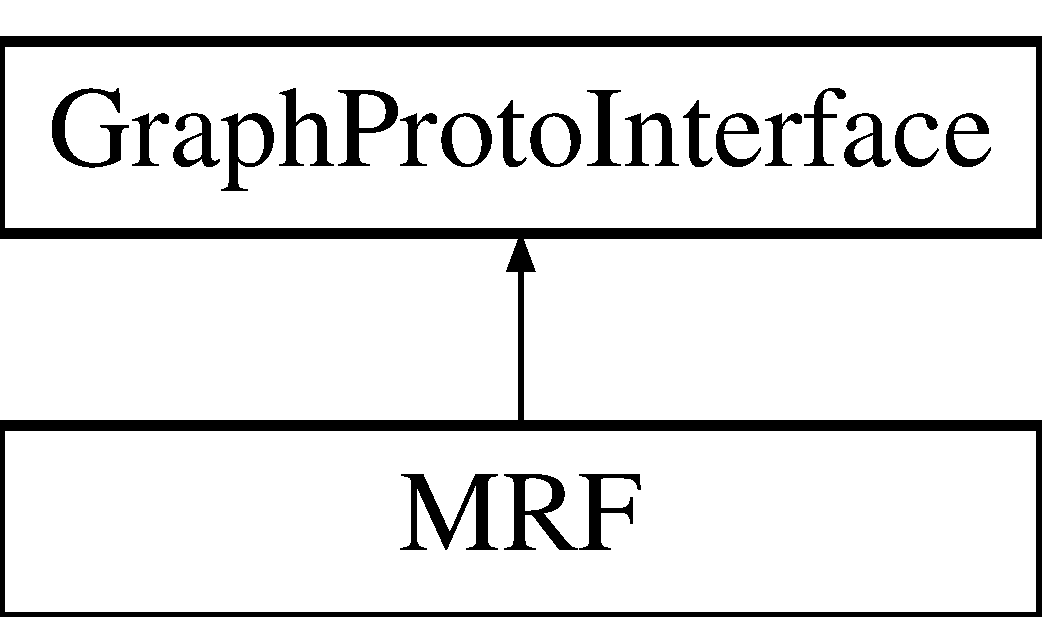
\includegraphics[height=2cm]{classGraphProtoInterface}
\end{center}
\end{figure}
\subsection*{Public Member Functions}
\begin{DoxyCompactItemize}
\item 
\hypertarget{classGraphProtoInterface_a4845501ec86ea627ce484cd78162c84c}{
void {\bfseries build\_\-from\_\-file} (const char $\ast$file\_\-name)}
\label{classGraphProtoInterface_a4845501ec86ea627ce484cd78162c84c}

\item 
\hypertarget{classGraphProtoInterface_a0dbd0905dbab167b9293d0ef32409af3}{
virtual void {\bfseries process\_\-node} (graph::Graph\_\-Node, \hyperlink{classScarab_1_1Graph_1_1Graphnode}{Graphnode} $\ast$)=0}
\label{classGraphProtoInterface_a0dbd0905dbab167b9293d0ef32409af3}

\item 
\hypertarget{classGraphProtoInterface_a3178c5f1eff8ed61d2512af8522cc550}{
virtual void {\bfseries process\_\-edge} (graph::Graph\_\-Edge, \hyperlink{classScarab_1_1Graph_1_1Graphedge}{Graphedge} $\ast$)=0}
\label{classGraphProtoInterface_a3178c5f1eff8ed61d2512af8522cc550}

\item 
\hypertarget{classGraphProtoInterface_a8b3125379c7b2bbf832b6b955496b76e}{
virtual void {\bfseries set\_\-up} (graph::Graph, int, int)}
\label{classGraphProtoInterface_a8b3125379c7b2bbf832b6b955496b76e}

\item 
\hypertarget{classGraphProtoInterface_a920e88785192db805206c875a8a3feed}{
const \hyperlink{classScarab_1_1Graph_1_1Graph}{Graph} \& {\bfseries graph} () const }
\label{classGraphProtoInterface_a920e88785192db805206c875a8a3feed}

\end{DoxyCompactItemize}
\subsection*{Public Attributes}
\begin{DoxyCompactItemize}
\item 
\hypertarget{classGraphProtoInterface_a8e262de0a3f65eaa20e5c528363bbb2a}{
\hyperlink{classScarab_1_1Graph_1_1Graph}{Graph} $\ast$ {\bfseries \_\-graph}}
\label{classGraphProtoInterface_a8e262de0a3f65eaa20e5c528363bbb2a}

\end{DoxyCompactItemize}


The documentation for this class was generated from the following files:\begin{DoxyCompactItemize}
\item 
graph/GraphProtoInterface.h\item 
graph/GraphProtoInterface.cpp\end{DoxyCompactItemize}

\hypertarget{classHardConstraints}{
\section{HardConstraints Class Reference}
\label{classHardConstraints}\index{HardConstraints@{HardConstraints}}
}
\subsection*{Public Member Functions}
\begin{DoxyCompactItemize}
\item 
\hypertarget{classHardConstraints_ad457a78e966e6ce3d71bfb3401b0300b}{
void {\bfseries read\_\-from\_\-file} (string file\_\-name)}
\label{classHardConstraints_ad457a78e966e6ce3d71bfb3401b0300b}

\item 
\hypertarget{classHardConstraints_a923f4ddd8b164d924147c22f054a9c7e}{
GRBLinExpr {\bfseries make\_\-lin\_\-expr} (const vector$<$ \hyperlink{structScarab_1_1HG_1_1DepParserLP}{DepParserLP} $\ast$ $>$ \&lp\_\-vars, const \hyperlink{structPossibleDep}{PossibleDep} \&dep)}
\label{classHardConstraints_a923f4ddd8b164d924147c22f054a9c7e}

\item 
\hypertarget{classHardConstraints_a0945fb67209be1cc95b31522d96e51cc}{
void {\bfseries show\_\-results} ()}
\label{classHardConstraints_a0945fb67209be1cc95b31522d96e51cc}

\item 
\hypertarget{classHardConstraints_a71ae98e67f5e5d3035aff1c2ef941a92}{
void {\bfseries add\_\-to\_\-lp} (const vector$<$ \hyperlink{structScarab_1_1HG_1_1DepParserLP}{DepParserLP} $\ast$ $>$ \&lp\_\-vars, GRBModel \&model)}
\label{classHardConstraints_a71ae98e67f5e5d3035aff1c2ef941a92}

\end{DoxyCompactItemize}
\subsection*{Public Attributes}
\begin{DoxyCompactItemize}
\item 
\hypertarget{classHardConstraints_ae0305e95d8065eb186ccae220b8e16f4}{
vector$<$ vector$<$ \hyperlink{structPossibleDep}{PossibleDep} $>$ $>$ {\bfseries \_\-constraint\_\-struct}}
\label{classHardConstraints_ae0305e95d8065eb186ccae220b8e16f4}

\item 
\hypertarget{classHardConstraints_a6b370ae5376bf283115092ab4bd33743}{
vector$<$ GRBVar $>$ {\bfseries group\_\-used}}
\label{classHardConstraints_a6b370ae5376bf283115092ab4bd33743}

\end{DoxyCompactItemize}


The documentation for this class was generated from the following file:\begin{DoxyCompactItemize}
\item 
lp/HardConstraints.h\end{DoxyCompactItemize}

\hypertarget{classHardPosConstraintsLP}{
\section{HardPosConstraintsLP Class Reference}
\label{classHardPosConstraintsLP}\index{HardPosConstraintsLP@{HardPosConstraintsLP}}
}
\subsection*{Public Member Functions}
\begin{DoxyCompactItemize}
\item 
\hypertarget{classHardPosConstraintsLP_a2979e37eb163b00f48a38ee8fccd1a64}{
{\bfseries HardPosConstraintsLP} (const \hyperlink{classTagConstraints}{TagConstraints} \&constraints, double penalty)}
\label{classHardPosConstraintsLP_a2979e37eb163b00f48a38ee8fccd1a64}

\item 
\hypertarget{classHardPosConstraintsLP_aa841ffcec001c0ee31714d0d39027c26}{
GRBLinExpr {\bfseries make\_\-lin\_\-expr} (const vector$<$ \hyperlink{structScarab_1_1HG_1_1TagLP}{TagLP} $\ast$ $>$ \&lp\_\-vars, const \hyperlink{structPossibleTag}{PossibleTag} \&tag, POS restricted\_\-to)}
\label{classHardPosConstraintsLP_aa841ffcec001c0ee31714d0d39027c26}

\item 
\hypertarget{classHardPosConstraintsLP_a7a7bb0c41351c9de3130045f0013c67b}{
void {\bfseries add\_\-to\_\-lp} (const vector$<$ \hyperlink{structScarab_1_1HG_1_1TagLP}{TagLP} $\ast$ $>$ \&lp\_\-vars, GRBModel \&model)}
\label{classHardPosConstraintsLP_a7a7bb0c41351c9de3130045f0013c67b}

\item 
\hypertarget{classHardPosConstraintsLP_a4307bcde1a701018736de348a718262b}{
void {\bfseries show\_\-results} ()}
\label{classHardPosConstraintsLP_a4307bcde1a701018736de348a718262b}

\end{DoxyCompactItemize}
\subsection*{Public Attributes}
\begin{DoxyCompactItemize}
\item 
\hypertarget{classHardPosConstraintsLP_a16ba65107e587a8cb43cc10949b0ebcf}{
vector$<$ vector$<$ GRBVar $>$ $>$ {\bfseries group\_\-used}}
\label{classHardPosConstraintsLP_a16ba65107e587a8cb43cc10949b0ebcf}

\item 
\hypertarget{classHardPosConstraintsLP_ad3b98e9e78140b02098420c674fcbaab}{
vector$<$ vector$<$ vector$<$ GRBVar $>$ $>$ $>$ {\bfseries slacks\_\-pos}}
\label{classHardPosConstraintsLP_ad3b98e9e78140b02098420c674fcbaab}

\item 
\hypertarget{classHardPosConstraintsLP_ac758c0971f82ef892f7f708db15bf472}{
vector$<$ vector$<$ vector$<$ GRBVar $>$ $>$ $>$ {\bfseries slacks\_\-neg}}
\label{classHardPosConstraintsLP_ac758c0971f82ef892f7f708db15bf472}

\item 
\hypertarget{classHardPosConstraintsLP_aa5c46efababe8dd5282a71ceb233c548}{
set$<$ int $>$ {\bfseries groups}}
\label{classHardPosConstraintsLP_aa5c46efababe8dd5282a71ceb233c548}

\end{DoxyCompactItemize}


The documentation for this class was generated from the following file:\begin{DoxyCompactItemize}
\item 
lp/HardPosConstraints.h\end{DoxyCompactItemize}

\hypertarget{classScarab_1_1HG_1_1Heuristic}{
\section{Scarab::HG::Heuristic Class Reference}
\label{classScarab_1_1HG_1_1Heuristic}\index{Scarab::HG::Heuristic@{Scarab::HG::Heuristic}}
}
Inheritance diagram for Scarab::HG::Heuristic:\begin{figure}[H]
\begin{center}
\leavevmode
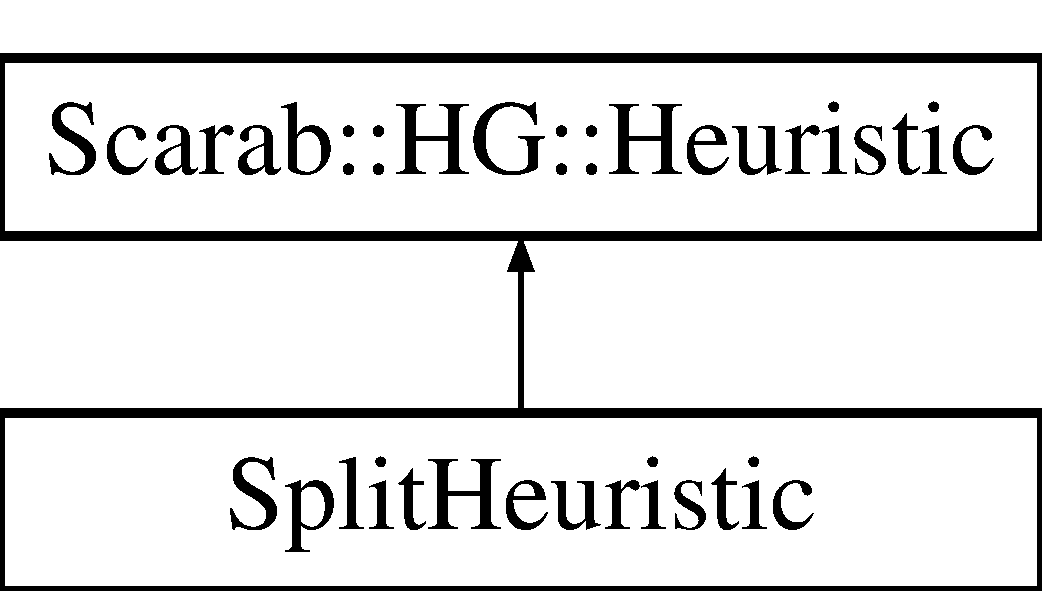
\includegraphics[height=2cm]{classScarab_1_1HG_1_1Heuristic}
\end{center}
\end{figure}
\subsection*{Public Member Functions}
\begin{DoxyCompactItemize}
\item 
\hypertarget{classScarab_1_1HG_1_1Heuristic_afad5a99d38b6783521e4c670d3edcf0a}{
virtual bool {\bfseries has\_\-value} (const \hyperlink{structScarab_1_1HG_1_1Location}{Location} \&loc, const \hyperlink{structScarab_1_1HG_1_1Hypothesis}{Hypothesis} \&hyp) const =0}
\label{classScarab_1_1HG_1_1Heuristic_afad5a99d38b6783521e4c670d3edcf0a}

\item 
\hypertarget{classScarab_1_1HG_1_1Heuristic_aca6b5924257b35be9e65058062fdc0d5}{
virtual double {\bfseries get\_\-value} (const \hyperlink{structScarab_1_1HG_1_1Location}{Location} \&loc, const \hyperlink{structScarab_1_1HG_1_1Hypothesis}{Hypothesis} \&hyp) const =0}
\label{classScarab_1_1HG_1_1Heuristic_aca6b5924257b35be9e65058062fdc0d5}

\end{DoxyCompactItemize}


The documentation for this class was generated from the following file:\begin{DoxyCompactItemize}
\item 
hypergraph/AStar.h\end{DoxyCompactItemize}

\hypertarget{classScarab_1_1HG_1_1HGraph}{
\section{Scarab::HG::HGraph Class Reference}
\label{classScarab_1_1HG_1_1HGraph}\index{Scarab::HG::HGraph@{Scarab::HG::HGraph}}
}
Inheritance diagram for Scarab::HG::HGraph:\begin{figure}[H]
\begin{center}
\leavevmode
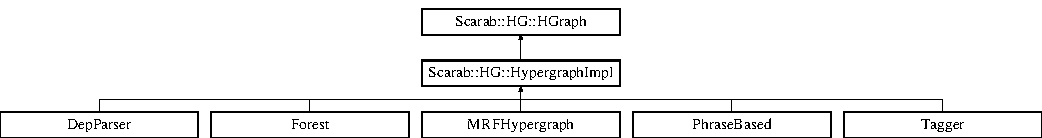
\includegraphics[height=1.85635cm]{classScarab_1_1HG_1_1HGraph}
\end{center}
\end{figure}
\subsection*{Public Member Functions}
\begin{DoxyCompactItemize}
\item 
virtual void \hyperlink{classScarab_1_1HG_1_1HGraph_ab5aa11c932b28864b56f28e0babbc1c1}{print} () const =0
\item 
virtual const \hyperlink{classScarab_1_1HG_1_1Hypernode}{Hypernode} \& \hyperlink{classScarab_1_1HG_1_1HGraph_a5ede392b158e41dd7e95ded1c4b0b5d6}{root} () const =0
\item 
\hypertarget{classScarab_1_1HG_1_1HGraph_a8309003db80be5bdbe4bb64f98a78ea8}{
virtual unsigned int {\bfseries num\_\-edges} () const =0}
\label{classScarab_1_1HG_1_1HGraph_a8309003db80be5bdbe4bb64f98a78ea8}

\item 
\hypertarget{classScarab_1_1HG_1_1HGraph_a6f4d37ef034cb38aa09c702b80a6e4f7}{
virtual unsigned int {\bfseries num\_\-nodes} () const =0}
\label{classScarab_1_1HG_1_1HGraph_a6f4d37ef034cb38aa09c702b80a6e4f7}

\item 
\hypertarget{classScarab_1_1HG_1_1HGraph_acad57dd952956b1a1a4367bba0e9383b}{
virtual const \hyperlink{classScarab_1_1HG_1_1Hypernode}{Hypernode} \& {\bfseries get\_\-node} (unsigned int i) const =0}
\label{classScarab_1_1HG_1_1HGraph_acad57dd952956b1a1a4367bba0e9383b}

\item 
\hypertarget{classScarab_1_1HG_1_1HGraph_aa599b296ae01affc9606f519e4e44e9e}{
virtual const \hyperlink{classScarab_1_1HG_1_1Hyperedge}{Hyperedge} \& {\bfseries get\_\-edge} (unsigned int i) const =0}
\label{classScarab_1_1HG_1_1HGraph_aa599b296ae01affc9606f519e4e44e9e}

\item 
virtual const vector$<$ \hyperlink{classScarab_1_1HG_1_1Hypernode}{Hypernode} $\ast$ $>$ \& \hyperlink{classScarab_1_1HG_1_1HGraph_a74d893fba015520774f71f02a46bb6ca}{nodes} () const =0
\item 
virtual const vector$<$ \hyperlink{classScarab_1_1HG_1_1Hyperedge}{Hyperedge} $\ast$ $>$ \& \hyperlink{classScarab_1_1HG_1_1HGraph_a57328729f90cc4152ca79ff15ecdd4bb}{edges} () const =0
\end{DoxyCompactItemize}


\subsection{Member Function Documentation}
\hypertarget{classScarab_1_1HG_1_1HGraph_a57328729f90cc4152ca79ff15ecdd4bb}{
\index{Scarab::HG::HGraph@{Scarab::HG::HGraph}!edges@{edges}}
\index{edges@{edges}!Scarab::HG::HGraph@{Scarab::HG::HGraph}}
\subsubsection[{edges}]{\setlength{\rightskip}{0pt plus 5cm}virtual const vector$<${\bf Hyperedge}$\ast$$>$\& Scarab::HG::HGraph::edges () const\hspace{0.3cm}{\ttfamily  \mbox{[}pure virtual\mbox{]}}}}
\label{classScarab_1_1HG_1_1HGraph_a57328729f90cc4152ca79ff15ecdd4bb}
Get all hyperedges in the hypergraph. (Assume unordered) WARNING: Treat this as a const iterator. \begin{DoxyReturn}{Returns}
Const iterator to edges in hypergraph . 
\end{DoxyReturn}


Implemented in \hyperlink{classScarab_1_1HG_1_1HypergraphImpl_a0c8373e545fe59b0cb7036b4751508e1}{Scarab::HG::HypergraphImpl}.

\hypertarget{classScarab_1_1HG_1_1HGraph_a74d893fba015520774f71f02a46bb6ca}{
\index{Scarab::HG::HGraph@{Scarab::HG::HGraph}!nodes@{nodes}}
\index{nodes@{nodes}!Scarab::HG::HGraph@{Scarab::HG::HGraph}}
\subsubsection[{nodes}]{\setlength{\rightskip}{0pt plus 5cm}virtual const vector$<${\bf Hypernode}$\ast$ $>$\& Scarab::HG::HGraph::nodes () const\hspace{0.3cm}{\ttfamily  \mbox{[}pure virtual\mbox{]}}}}
\label{classScarab_1_1HG_1_1HGraph_a74d893fba015520774f71f02a46bb6ca}
Get all hypernodes in the hypergraph. (Assume unordered) WARNING: Treat this as a const iterator. \begin{DoxyReturn}{Returns}
Const iterator to hypernodes in hypergraph . 
\end{DoxyReturn}


Implemented in \hyperlink{classScarab_1_1HG_1_1HypergraphImpl_a9aef2881b489c86d4d83e996a70f8141}{Scarab::HG::HypergraphImpl}.

\hypertarget{classScarab_1_1HG_1_1HGraph_ab5aa11c932b28864b56f28e0babbc1c1}{
\index{Scarab::HG::HGraph@{Scarab::HG::HGraph}!print@{print}}
\index{print@{print}!Scarab::HG::HGraph@{Scarab::HG::HGraph}}
\subsubsection[{print}]{\setlength{\rightskip}{0pt plus 5cm}virtual void Scarab::HG::HGraph::print () const\hspace{0.3cm}{\ttfamily  \mbox{[}pure virtual\mbox{]}}}}
\label{classScarab_1_1HG_1_1HGraph_ab5aa11c932b28864b56f28e0babbc1c1}
Display the hypergraph for debugging. 

Implemented in \hyperlink{classMRFHypergraph_aaac6b68c3ece41ddd1f8107e961879bc}{MRFHypergraph}, \hyperlink{classDepParser_a9aebbbde821bad423b6c01cc12f02a2c}{DepParser}, \hyperlink{classPhraseBased_aafc2997b58b3698fed7cb5a1f6f269c6}{PhraseBased}, \hyperlink{classTagger_a4ebe0aebd7c0392970b401a5a6c6cd72}{Tagger}, and \hyperlink{classForest_a621a1a65d0f877bb33b15c79f9e24c4d}{Forest}.

\hypertarget{classScarab_1_1HG_1_1HGraph_a5ede392b158e41dd7e95ded1c4b0b5d6}{
\index{Scarab::HG::HGraph@{Scarab::HG::HGraph}!root@{root}}
\index{root@{root}!Scarab::HG::HGraph@{Scarab::HG::HGraph}}
\subsubsection[{root}]{\setlength{\rightskip}{0pt plus 5cm}virtual const {\bf Hypernode}\& Scarab::HG::HGraph::root () const\hspace{0.3cm}{\ttfamily  \mbox{[}pure virtual\mbox{]}}}}
\label{classScarab_1_1HG_1_1HGraph_a5ede392b158e41dd7e95ded1c4b0b5d6}
Get the root of the hypergraph

\begin{DoxyReturn}{Returns}
\hyperlink{classScarab_1_1HG_1_1Hypernode}{Hypernode} at root 
\end{DoxyReturn}


Implemented in \hyperlink{classScarab_1_1HG_1_1HypergraphImpl_a31172009b97d179f6b1199f191197a32}{Scarab::HG::HypergraphImpl}.



The documentation for this class was generated from the following file:\begin{DoxyCompactItemize}
\item 
hypergraph/Hypergraph.h\end{DoxyCompactItemize}

\hypertarget{structHyp}{
\section{Hyp Struct Reference}
\label{structHyp}\index{Hyp@{Hyp}}
}
\subsection*{Public Member Functions}
\begin{DoxyCompactItemize}
\item 
\hypertarget{structHyp_a5fba7860265cf935133e4c0c73fec090}{
{\bfseries Hyp} (double score\_\-in, Sig sig\_\-in, vector$<$ int $>$ full\_\-der)}
\label{structHyp_a5fba7860265cf935133e4c0c73fec090}

\item 
\hypertarget{structHyp_a547883a1aa9a7573d328d0f6b385dca8}{
bool {\bfseries operator$<$} (const \hyperlink{structHyp}{Hyp} \&other) const }
\label{structHyp_a547883a1aa9a7573d328d0f6b385dca8}

\end{DoxyCompactItemize}
\subsection*{Public Attributes}
\begin{DoxyCompactItemize}
\item 
\hypertarget{structHyp_a7d24c5a317140b8050dc57255bb7922a}{
double {\bfseries score}}
\label{structHyp_a7d24c5a317140b8050dc57255bb7922a}

\item 
\hypertarget{structHyp_a4aa96a03dc6b82416074985e0ecd39c3}{
Sig {\bfseries sig}}
\label{structHyp_a4aa96a03dc6b82416074985e0ecd39c3}

\item 
\hypertarget{structHyp_a076825f81d94a1f2b20bb5141eb9f4c7}{
vector$<$ int $>$ {\bfseries full\_\-derivation}}
\label{structHyp_a076825f81d94a1f2b20bb5141eb9f4c7}

\end{DoxyCompactItemize}


The documentation for this struct was generated from the following file:\begin{DoxyCompactItemize}
\item 
hypergraph/CubePruning.h\end{DoxyCompactItemize}

\hypertarget{classScarab_1_1HG_1_1Hyperedge}{
\section{Scarab::HG::Hyperedge Class Reference}
\label{classScarab_1_1HG_1_1Hyperedge}\index{Scarab::HG::Hyperedge@{Scarab::HG::Hyperedge}}
}
Inheritance diagram for Scarab::HG::Hyperedge:\begin{figure}[H]
\begin{center}
\leavevmode
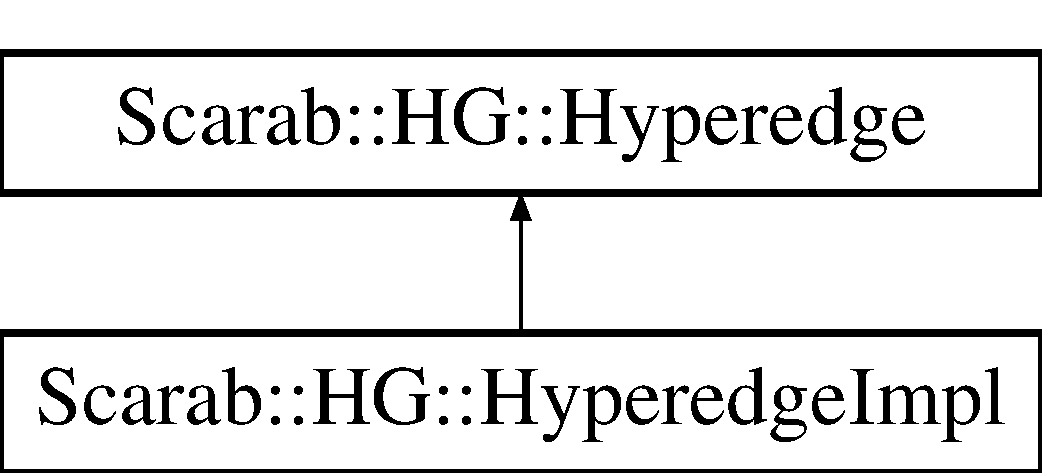
\includegraphics[height=2cm]{classScarab_1_1HG_1_1Hyperedge}
\end{center}
\end{figure}
\subsection*{Public Member Functions}
\begin{DoxyCompactItemize}
\item 
virtual unsigned int \hyperlink{classScarab_1_1HG_1_1Hyperedge_af824beb7107253a7545b35992c17e057}{id} () const =0
\item 
\hypertarget{classScarab_1_1HG_1_1Hyperedge_a8442c017fcee87c1f865b2254b49900f}{
virtual string {\bfseries label} () const =0}
\label{classScarab_1_1HG_1_1Hyperedge_a8442c017fcee87c1f865b2254b49900f}

\item 
virtual const \hyperlink{classScarab_1_1HG_1_1Hypernode}{Hypernode} \& \hyperlink{classScarab_1_1HG_1_1Hyperedge_a9ec8cf9ea7b5f762f359a6f9f1c038da}{tail\_\-node} (unsigned int i) const =0
\item 
virtual unsigned int \hyperlink{classScarab_1_1HG_1_1Hyperedge_a799d8d98242c129d7eee178bdf1fb535}{num\_\-nodes} () const =0
\item 
virtual const svector$<$ int, double $>$ \& \hyperlink{classScarab_1_1HG_1_1Hyperedge_a0d201ddb955631aadee4c15cc8e709f8}{fvector} () const =0
\item 
virtual const \hyperlink{classScarab_1_1HG_1_1Hypernode}{Hypernode} \& \hyperlink{classScarab_1_1HG_1_1Hyperedge_a6043de341070c103d811f5286193dd46}{head\_\-node} () const =0
\item 
virtual const vector$<$ \hyperlink{classScarab_1_1HG_1_1Hypernode}{Hypernode} $\ast$ $>$ \& \hyperlink{classScarab_1_1HG_1_1Hyperedge_abac6d27691186608aa12949de6e1c283}{tail\_\-nodes} () const =0
\end{DoxyCompactItemize}


\subsection{Member Function Documentation}
\hypertarget{classScarab_1_1HG_1_1Hyperedge_a0d201ddb955631aadee4c15cc8e709f8}{
\index{Scarab::HG::Hyperedge@{Scarab::HG::Hyperedge}!fvector@{fvector}}
\index{fvector@{fvector}!Scarab::HG::Hyperedge@{Scarab::HG::Hyperedge}}
\subsubsection[{fvector}]{\setlength{\rightskip}{0pt plus 5cm}virtual const svector$<$int, double$>$\& Scarab::HG::Hyperedge::fvector () const\hspace{0.3cm}{\ttfamily  \mbox{[}pure virtual\mbox{]}}}}
\label{classScarab_1_1HG_1_1Hyperedge_a0d201ddb955631aadee4c15cc8e709f8}
The feature vector associated with this node. TODO: remove this from the representation \begin{Desc}
\item[\hyperlink{deprecated__deprecated000005}{Deprecated}]\end{Desc}
\begin{DoxyReturn}{Returns}
Feature vector 
\end{DoxyReturn}


Implemented in \hyperlink{classScarab_1_1HG_1_1HyperedgeImpl_a359446c285164a93995bb87e6ea74882}{Scarab::HG::HyperedgeImpl}.

\hypertarget{classScarab_1_1HG_1_1Hyperedge_a6043de341070c103d811f5286193dd46}{
\index{Scarab::HG::Hyperedge@{Scarab::HG::Hyperedge}!head\_\-node@{head\_\-node}}
\index{head\_\-node@{head\_\-node}!Scarab::HG::Hyperedge@{Scarab::HG::Hyperedge}}
\subsubsection[{head\_\-node}]{\setlength{\rightskip}{0pt plus 5cm}virtual const {\bf Hypernode}\& Scarab::HG::Hyperedge::head\_\-node () const\hspace{0.3cm}{\ttfamily  \mbox{[}pure virtual\mbox{]}}}}
\label{classScarab_1_1HG_1_1Hyperedge_a6043de341070c103d811f5286193dd46}
Get the node at the head of this hyperedge

\begin{DoxyReturn}{Returns}
Head node 
\end{DoxyReturn}


Implemented in \hyperlink{classScarab_1_1HG_1_1HyperedgeImpl_ae194bfc8ecac2a12791fa36c1c2c62a7}{Scarab::HG::HyperedgeImpl}.

\hypertarget{classScarab_1_1HG_1_1Hyperedge_af824beb7107253a7545b35992c17e057}{
\index{Scarab::HG::Hyperedge@{Scarab::HG::Hyperedge}!id@{id}}
\index{id@{id}!Scarab::HG::Hyperedge@{Scarab::HG::Hyperedge}}
\subsubsection[{id}]{\setlength{\rightskip}{0pt plus 5cm}virtual unsigned int Scarab::HG::Hyperedge::id () const\hspace{0.3cm}{\ttfamily  \mbox{[}pure virtual\mbox{]}}}}
\label{classScarab_1_1HG_1_1Hyperedge_af824beb7107253a7545b35992c17e057}
Get edge id

\begin{DoxyReturn}{Returns}
The id of this edge in a fixed hypergraph 
\end{DoxyReturn}


Implemented in \hyperlink{classScarab_1_1HG_1_1HyperedgeImpl_afa81943347267781c25c4e68f7f5f547}{Scarab::HG::HyperedgeImpl}.

\hypertarget{classScarab_1_1HG_1_1Hyperedge_a799d8d98242c129d7eee178bdf1fb535}{
\index{Scarab::HG::Hyperedge@{Scarab::HG::Hyperedge}!num\_\-nodes@{num\_\-nodes}}
\index{num\_\-nodes@{num\_\-nodes}!Scarab::HG::Hyperedge@{Scarab::HG::Hyperedge}}
\subsubsection[{num\_\-nodes}]{\setlength{\rightskip}{0pt plus 5cm}virtual unsigned int Scarab::HG::Hyperedge::num\_\-nodes () const\hspace{0.3cm}{\ttfamily  \mbox{[}pure virtual\mbox{]}}}}
\label{classScarab_1_1HG_1_1Hyperedge_a799d8d98242c129d7eee178bdf1fb535}
The number of tail nodes in this edge. \begin{Desc}
\item[\hyperlink{deprecated__deprecated000004}{Deprecated}]\end{Desc}
\begin{DoxyReturn}{Returns}
The length 
\end{DoxyReturn}


Implemented in \hyperlink{classScarab_1_1HG_1_1HyperedgeImpl_a9a5bef8789c9c7caee6f53833ea4acc7}{Scarab::HG::HyperedgeImpl}.

\hypertarget{classScarab_1_1HG_1_1Hyperedge_a9ec8cf9ea7b5f762f359a6f9f1c038da}{
\index{Scarab::HG::Hyperedge@{Scarab::HG::Hyperedge}!tail\_\-node@{tail\_\-node}}
\index{tail\_\-node@{tail\_\-node}!Scarab::HG::Hyperedge@{Scarab::HG::Hyperedge}}
\subsubsection[{tail\_\-node}]{\setlength{\rightskip}{0pt plus 5cm}virtual const {\bf Hypernode}\& Scarab::HG::Hyperedge::tail\_\-node (unsigned int {\em i}) const\hspace{0.3cm}{\ttfamily  \mbox{[}pure virtual\mbox{]}}}}
\label{classScarab_1_1HG_1_1Hyperedge_a9ec8cf9ea7b5f762f359a6f9f1c038da}
Get a node in this edges tail \begin{Desc}
\item[\hyperlink{deprecated__deprecated000003}{Deprecated}]\end{Desc}

\begin{DoxyParams}{Parameters}
\item[{\em i}]The node position, in tail\_\-node order\end{DoxyParams}
\begin{DoxyReturn}{Returns}
The hypernode 
\end{DoxyReturn}


Implemented in \hyperlink{classScarab_1_1HG_1_1HyperedgeImpl_a7087ba121f3056eb5946d1909c4b3d58}{Scarab::HG::HyperedgeImpl}.

\hypertarget{classScarab_1_1HG_1_1Hyperedge_abac6d27691186608aa12949de6e1c283}{
\index{Scarab::HG::Hyperedge@{Scarab::HG::Hyperedge}!tail\_\-nodes@{tail\_\-nodes}}
\index{tail\_\-nodes@{tail\_\-nodes}!Scarab::HG::Hyperedge@{Scarab::HG::Hyperedge}}
\subsubsection[{tail\_\-nodes}]{\setlength{\rightskip}{0pt plus 5cm}virtual const vector$<${\bf Hypernode} $\ast$$>$\& Scarab::HG::Hyperedge::tail\_\-nodes () const\hspace{0.3cm}{\ttfamily  \mbox{[}pure virtual\mbox{]}}}}
\label{classScarab_1_1HG_1_1Hyperedge_abac6d27691186608aa12949de6e1c283}
Get all the nodes in the tail of the hyperedge WARNING: Treat this as a const iterator. \begin{DoxyReturn}{Returns}
Const iterator to nodes. 
\end{DoxyReturn}


Implemented in \hyperlink{classScarab_1_1HG_1_1HyperedgeImpl_a3bf00c8c032397150f59e196aea5e245}{Scarab::HG::HyperedgeImpl}.



The documentation for this class was generated from the following file:\begin{DoxyCompactItemize}
\item 
hypergraph/Hypergraph.h\end{DoxyCompactItemize}

\hypertarget{classScarab_1_1HG_1_1HyperedgeImpl}{
\section{Scarab::HG::HyperedgeImpl Class Reference}
\label{classScarab_1_1HG_1_1HyperedgeImpl}\index{Scarab::HG::HyperedgeImpl@{Scarab::HG::HyperedgeImpl}}
}
Inheritance diagram for Scarab::HG::HyperedgeImpl:\begin{figure}[H]
\begin{center}
\leavevmode
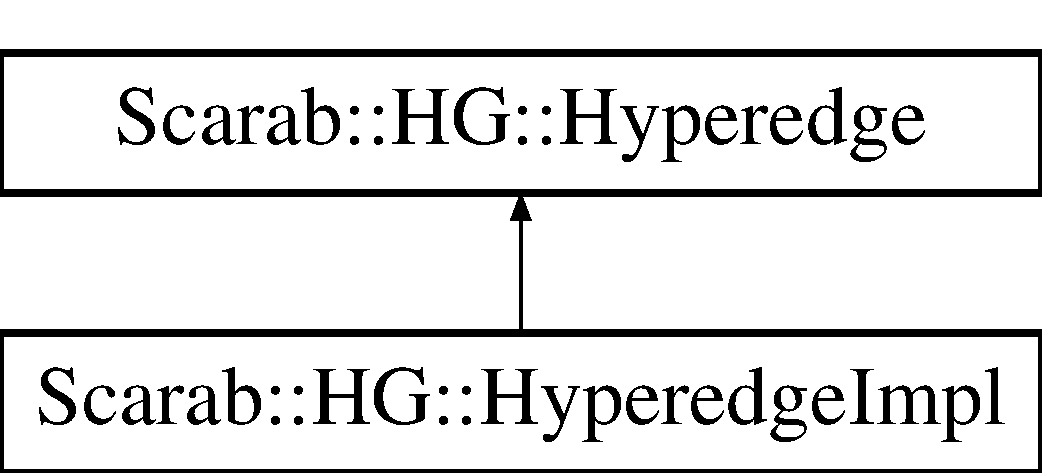
\includegraphics[height=2cm]{classScarab_1_1HG_1_1HyperedgeImpl}
\end{center}
\end{figure}
\subsection*{Public Member Functions}
\begin{DoxyCompactItemize}
\item 
\hypertarget{classScarab_1_1HG_1_1HyperedgeImpl_a3c141efe1be2e8ee78d45caca4711c6e}{
{\bfseries HyperedgeImpl} (const string \&label, str\_\-vector $\ast$features, int id, vector$<$ \hyperlink{classScarab_1_1HG_1_1Hypernode}{Hypernode} $\ast$ $>$ tail\_\-nodes, \hyperlink{classScarab_1_1HG_1_1Hypernode}{Hypernode} $\ast$head\_\-node)}
\label{classScarab_1_1HG_1_1HyperedgeImpl_a3c141efe1be2e8ee78d45caca4711c6e}

\item 
const \hyperlink{classScarab_1_1HG_1_1Hypernode}{Hypernode} \& \hyperlink{classScarab_1_1HG_1_1HyperedgeImpl_a7087ba121f3056eb5946d1909c4b3d58}{tail\_\-node} (unsigned int i) const 
\item 
uint \hyperlink{classScarab_1_1HG_1_1HyperedgeImpl_a9a5bef8789c9c7caee6f53833ea4acc7}{num\_\-nodes} () const 
\item 
const wvector \& \hyperlink{classScarab_1_1HG_1_1HyperedgeImpl_a359446c285164a93995bb87e6ea74882}{fvector} () const 
\item 
const \hyperlink{classScarab_1_1HG_1_1Hypernode}{Scarab::HG::Hypernode} \& \hyperlink{classScarab_1_1HG_1_1HyperedgeImpl_ae194bfc8ecac2a12791fa36c1c2c62a7}{head\_\-node} () const 
\item 
const vector$<$ \hyperlink{classScarab_1_1HG_1_1Hypernode}{Scarab::HG::Hypernode} $\ast$ $>$ \& \hyperlink{classScarab_1_1HG_1_1HyperedgeImpl_a3bf00c8c032397150f59e196aea5e245}{tail\_\-nodes} () const 
\item 
uint \hyperlink{classScarab_1_1HG_1_1HyperedgeImpl_afa81943347267781c25c4e68f7f5f547}{id} () const 
\item 
\hypertarget{classScarab_1_1HG_1_1HyperedgeImpl_a8fe687c9914de37c4d91c353ba669665}{
string {\bfseries label} () const }
\label{classScarab_1_1HG_1_1HyperedgeImpl_a8fe687c9914de37c4d91c353ba669665}

\item 
\hypertarget{classScarab_1_1HG_1_1HyperedgeImpl_a068e4291cbcaa68a59ad64ede34f9edc}{
void {\bfseries reid} (int new\_\-id)}
\label{classScarab_1_1HG_1_1HyperedgeImpl_a068e4291cbcaa68a59ad64ede34f9edc}

\end{DoxyCompactItemize}
\subsection*{Public Attributes}
\begin{DoxyCompactItemize}
\item 
\hypertarget{classScarab_1_1HG_1_1HyperedgeImpl_ab14180934c56806b0004bcbdac9eef88}{
const string {\bfseries \_\-label}}
\label{classScarab_1_1HG_1_1HyperedgeImpl_ab14180934c56806b0004bcbdac9eef88}

\item 
\hypertarget{classScarab_1_1HG_1_1HyperedgeImpl_a70fab435c66aab79825aab6b9058cda5}{
vector$<$ \hyperlink{classScarab_1_1HG_1_1Hypernode}{Hypernode} $\ast$ $>$ {\bfseries \_\-tail\_\-nodes}}
\label{classScarab_1_1HG_1_1HyperedgeImpl_a70fab435c66aab79825aab6b9058cda5}

\item 
\hypertarget{classScarab_1_1HG_1_1HyperedgeImpl_a92aeb9593a64be769f18666c3bfd0a20}{
\hyperlink{classScarab_1_1HG_1_1Hypernode}{Hypernode} $\ast$ {\bfseries \_\-head\_\-node}}
\label{classScarab_1_1HG_1_1HyperedgeImpl_a92aeb9593a64be769f18666c3bfd0a20}

\end{DoxyCompactItemize}


\subsection{Member Function Documentation}
\hypertarget{classScarab_1_1HG_1_1HyperedgeImpl_a359446c285164a93995bb87e6ea74882}{
\index{Scarab::HG::HyperedgeImpl@{Scarab::HG::HyperedgeImpl}!fvector@{fvector}}
\index{fvector@{fvector}!Scarab::HG::HyperedgeImpl@{Scarab::HG::HyperedgeImpl}}
\subsubsection[{fvector}]{\setlength{\rightskip}{0pt plus 5cm}const wvector\& Scarab::HG::HyperedgeImpl::fvector () const\hspace{0.3cm}{\ttfamily  \mbox{[}inline, virtual\mbox{]}}}}
\label{classScarab_1_1HG_1_1HyperedgeImpl_a359446c285164a93995bb87e6ea74882}
The feature vector associated with this node. TODO: remove this from the representation \begin{Desc}
\item[\hyperlink{deprecated__deprecated000005}{Deprecated}]\end{Desc}
\begin{DoxyReturn}{Returns}
Feature vector 
\end{DoxyReturn}


Implements \hyperlink{classScarab_1_1HG_1_1Hyperedge_a0d201ddb955631aadee4c15cc8e709f8}{Scarab::HG::Hyperedge}.

\hypertarget{classScarab_1_1HG_1_1HyperedgeImpl_ae194bfc8ecac2a12791fa36c1c2c62a7}{
\index{Scarab::HG::HyperedgeImpl@{Scarab::HG::HyperedgeImpl}!head\_\-node@{head\_\-node}}
\index{head\_\-node@{head\_\-node}!Scarab::HG::HyperedgeImpl@{Scarab::HG::HyperedgeImpl}}
\subsubsection[{head\_\-node}]{\setlength{\rightskip}{0pt plus 5cm}const {\bf Scarab::HG::Hypernode}\& Scarab::HG::HyperedgeImpl::head\_\-node () const\hspace{0.3cm}{\ttfamily  \mbox{[}inline, virtual\mbox{]}}}}
\label{classScarab_1_1HG_1_1HyperedgeImpl_ae194bfc8ecac2a12791fa36c1c2c62a7}
Get the node at the head of this hyperedge

\begin{DoxyReturn}{Returns}
Head node 
\end{DoxyReturn}


Implements \hyperlink{classScarab_1_1HG_1_1Hyperedge_a6043de341070c103d811f5286193dd46}{Scarab::HG::Hyperedge}.

\hypertarget{classScarab_1_1HG_1_1HyperedgeImpl_afa81943347267781c25c4e68f7f5f547}{
\index{Scarab::HG::HyperedgeImpl@{Scarab::HG::HyperedgeImpl}!id@{id}}
\index{id@{id}!Scarab::HG::HyperedgeImpl@{Scarab::HG::HyperedgeImpl}}
\subsubsection[{id}]{\setlength{\rightskip}{0pt plus 5cm}uint Scarab::HG::HyperedgeImpl::id () const\hspace{0.3cm}{\ttfamily  \mbox{[}inline, virtual\mbox{]}}}}
\label{classScarab_1_1HG_1_1HyperedgeImpl_afa81943347267781c25c4e68f7f5f547}
Get edge id

\begin{DoxyReturn}{Returns}
The id of this edge in a fixed hypergraph 
\end{DoxyReturn}


Implements \hyperlink{classScarab_1_1HG_1_1Hyperedge_af824beb7107253a7545b35992c17e057}{Scarab::HG::Hyperedge}.

\hypertarget{classScarab_1_1HG_1_1HyperedgeImpl_a9a5bef8789c9c7caee6f53833ea4acc7}{
\index{Scarab::HG::HyperedgeImpl@{Scarab::HG::HyperedgeImpl}!num\_\-nodes@{num\_\-nodes}}
\index{num\_\-nodes@{num\_\-nodes}!Scarab::HG::HyperedgeImpl@{Scarab::HG::HyperedgeImpl}}
\subsubsection[{num\_\-nodes}]{\setlength{\rightskip}{0pt plus 5cm}uint Scarab::HG::HyperedgeImpl::num\_\-nodes () const\hspace{0.3cm}{\ttfamily  \mbox{[}inline, virtual\mbox{]}}}}
\label{classScarab_1_1HG_1_1HyperedgeImpl_a9a5bef8789c9c7caee6f53833ea4acc7}
The number of tail nodes in this edge. \begin{Desc}
\item[\hyperlink{deprecated__deprecated000004}{Deprecated}]\end{Desc}
\begin{DoxyReturn}{Returns}
The length 
\end{DoxyReturn}


Implements \hyperlink{classScarab_1_1HG_1_1Hyperedge_a799d8d98242c129d7eee178bdf1fb535}{Scarab::HG::Hyperedge}.

\hypertarget{classScarab_1_1HG_1_1HyperedgeImpl_a7087ba121f3056eb5946d1909c4b3d58}{
\index{Scarab::HG::HyperedgeImpl@{Scarab::HG::HyperedgeImpl}!tail\_\-node@{tail\_\-node}}
\index{tail\_\-node@{tail\_\-node}!Scarab::HG::HyperedgeImpl@{Scarab::HG::HyperedgeImpl}}
\subsubsection[{tail\_\-node}]{\setlength{\rightskip}{0pt plus 5cm}const {\bf Hypernode}\& Scarab::HG::HyperedgeImpl::tail\_\-node (unsigned int {\em i}) const\hspace{0.3cm}{\ttfamily  \mbox{[}inline, virtual\mbox{]}}}}
\label{classScarab_1_1HG_1_1HyperedgeImpl_a7087ba121f3056eb5946d1909c4b3d58}
Get a node in this edges tail \begin{Desc}
\item[\hyperlink{deprecated__deprecated000003}{Deprecated}]\end{Desc}

\begin{DoxyParams}{Parameters}
\item[{\em i}]The node position, in tail\_\-node order\end{DoxyParams}
\begin{DoxyReturn}{Returns}
The hypernode 
\end{DoxyReturn}


Implements \hyperlink{classScarab_1_1HG_1_1Hyperedge_a9ec8cf9ea7b5f762f359a6f9f1c038da}{Scarab::HG::Hyperedge}.

\hypertarget{classScarab_1_1HG_1_1HyperedgeImpl_a3bf00c8c032397150f59e196aea5e245}{
\index{Scarab::HG::HyperedgeImpl@{Scarab::HG::HyperedgeImpl}!tail\_\-nodes@{tail\_\-nodes}}
\index{tail\_\-nodes@{tail\_\-nodes}!Scarab::HG::HyperedgeImpl@{Scarab::HG::HyperedgeImpl}}
\subsubsection[{tail\_\-nodes}]{\setlength{\rightskip}{0pt plus 5cm}const vector$<${\bf Scarab::HG::Hypernode}$\ast$$>$\& Scarab::HG::HyperedgeImpl::tail\_\-nodes () const\hspace{0.3cm}{\ttfamily  \mbox{[}inline, virtual\mbox{]}}}}
\label{classScarab_1_1HG_1_1HyperedgeImpl_a3bf00c8c032397150f59e196aea5e245}
Get all the nodes in the tail of the hyperedge WARNING: Treat this as a const iterator. \begin{DoxyReturn}{Returns}
Const iterator to nodes. 
\end{DoxyReturn}


Implements \hyperlink{classScarab_1_1HG_1_1Hyperedge_abac6d27691186608aa12949de6e1c283}{Scarab::HG::Hyperedge}.



The documentation for this class was generated from the following file:\begin{DoxyCompactItemize}
\item 
hypergraph/HypergraphImpl.h\end{DoxyCompactItemize}

\hypertarget{classHypergraph}{
\section{Hypergraph Class Reference}
\label{classHypergraph}\index{Hypergraph@{Hypergraph}}
}
\subsection*{Public Types}
\begin{DoxyCompactItemize}
\item 
\hypertarget{classHypergraph_a36c26b747a86e20cc9e7b0ce733fe38a}{
typedef \hyperlink{classHypergraph__Node}{Hypergraph\_\-Node} {\bfseries Node}}
\label{classHypergraph_a36c26b747a86e20cc9e7b0ce733fe38a}

\item 
\hypertarget{classHypergraph_a8161caf487c105fff5e3ffd589ed176f}{
typedef \hyperlink{classHypergraph__Edge}{Hypergraph\_\-Edge} {\bfseries Edge}}
\label{classHypergraph_a8161caf487c105fff5e3ffd589ed176f}

\item 
\hypertarget{classHypergraph_a36c26b747a86e20cc9e7b0ce733fe38a}{
typedef \hyperlink{classHypergraph__Node}{Hypergraph\_\-Node} {\bfseries Node}}
\label{classHypergraph_a36c26b747a86e20cc9e7b0ce733fe38a}

\item 
\hypertarget{classHypergraph_a8161caf487c105fff5e3ffd589ed176f}{
typedef \hyperlink{classHypergraph__Edge}{Hypergraph\_\-Edge} {\bfseries Edge}}
\label{classHypergraph_a8161caf487c105fff5e3ffd589ed176f}

\end{DoxyCompactItemize}
\subsection*{Public Member Functions}
\begin{DoxyCompactItemize}
\item 
\hypertarget{classHypergraph_aa5b69fea3073cbbc6230c403aba60a13}{
{\bfseries Hypergraph} (const \hyperlink{classHypergraph}{Hypergraph} \&from)}
\label{classHypergraph_aa5b69fea3073cbbc6230c403aba60a13}

\item 
\hypertarget{classHypergraph_a6fa4366f554df3ffd7aa3694a3612006}{
\hyperlink{classHypergraph}{Hypergraph} \& {\bfseries operator=} (const \hyperlink{classHypergraph}{Hypergraph} \&from)}
\label{classHypergraph_a6fa4366f554df3ffd7aa3694a3612006}

\item 
\hypertarget{classHypergraph_a20ec2be2fda0e1db366f26c95817cd89}{
const ::google::protobuf::UnknownFieldSet \& {\bfseries unknown\_\-fields} () const }
\label{classHypergraph_a20ec2be2fda0e1db366f26c95817cd89}

\item 
\hypertarget{classHypergraph_a423987a46404cd3221a5c4035050b4b8}{
inline::google::protobuf::UnknownFieldSet $\ast$ {\bfseries mutable\_\-unknown\_\-fields} ()}
\label{classHypergraph_a423987a46404cd3221a5c4035050b4b8}

\item 
\hypertarget{classHypergraph_ac4a85460aabebe97e0411a30d80f720d}{
void {\bfseries Swap} (\hyperlink{classHypergraph}{Hypergraph} $\ast$other)}
\label{classHypergraph_ac4a85460aabebe97e0411a30d80f720d}

\item 
\hypertarget{classHypergraph_aed1ca8c3f4626f4313cd7e1b1ebf2676}{
\hyperlink{classHypergraph}{Hypergraph} $\ast$ {\bfseries New} () const }
\label{classHypergraph_aed1ca8c3f4626f4313cd7e1b1ebf2676}

\item 
\hypertarget{classHypergraph_a344289a1a02daaa7e9bb2284507bc25b}{
void {\bfseries CopyFrom} (const ::google::protobuf::Message \&from)}
\label{classHypergraph_a344289a1a02daaa7e9bb2284507bc25b}

\item 
\hypertarget{classHypergraph_a4aafea60a0bf75fe2c2f66172101110b}{
void {\bfseries MergeFrom} (const ::google::protobuf::Message \&from)}
\label{classHypergraph_a4aafea60a0bf75fe2c2f66172101110b}

\item 
\hypertarget{classHypergraph_a4715ac922c373c335985c25f9766a526}{
void {\bfseries CopyFrom} (const \hyperlink{classHypergraph}{Hypergraph} \&from)}
\label{classHypergraph_a4715ac922c373c335985c25f9766a526}

\item 
\hypertarget{classHypergraph_a5e48c533c90271a6e018a26ac8a70538}{
void {\bfseries MergeFrom} (const \hyperlink{classHypergraph}{Hypergraph} \&from)}
\label{classHypergraph_a5e48c533c90271a6e018a26ac8a70538}

\item 
\hypertarget{classHypergraph_a3377b5de90d222621cc41c2c41b7865d}{
void {\bfseries Clear} ()}
\label{classHypergraph_a3377b5de90d222621cc41c2c41b7865d}

\item 
\hypertarget{classHypergraph_a5327b9372e5dd8dd4e435b160e5f16df}{
bool {\bfseries IsInitialized} () const }
\label{classHypergraph_a5327b9372e5dd8dd4e435b160e5f16df}

\item 
\hypertarget{classHypergraph_ab4aa8a83cd1da71a9f31bdad594ffaf0}{
int {\bfseries ByteSize} () const }
\label{classHypergraph_ab4aa8a83cd1da71a9f31bdad594ffaf0}

\item 
\hypertarget{classHypergraph_a30583bfba242ae1439903bc24d069e24}{
bool {\bfseries MergePartialFromCodedStream} (::google::protobuf::io::CodedInputStream $\ast$input)}
\label{classHypergraph_a30583bfba242ae1439903bc24d069e24}

\item 
\hypertarget{classHypergraph_a7e8e7f4fe037cbfeb1f0a46e7616fc78}{
void {\bfseries SerializeWithCachedSizes} (::google::protobuf::io::CodedOutputStream $\ast$output) const }
\label{classHypergraph_a7e8e7f4fe037cbfeb1f0a46e7616fc78}

\item 
\hypertarget{classHypergraph_a4d695da7efbbcc2444fb1836e88d8849}{
::google::protobuf::uint8 $\ast$ {\bfseries SerializeWithCachedSizesToArray} (::google::protobuf::uint8 $\ast$output) const }
\label{classHypergraph_a4d695da7efbbcc2444fb1836e88d8849}

\item 
\hypertarget{classHypergraph_a34d579551c68eb5e039062269f875522}{
int {\bfseries GetCachedSize} () const }
\label{classHypergraph_a34d579551c68eb5e039062269f875522}

\item 
\hypertarget{classHypergraph_a5e8ebd56fb4cdfcaa19b9aa43cf25fbd}{
::google::protobuf::Metadata {\bfseries GetMetadata} () const }
\label{classHypergraph_a5e8ebd56fb4cdfcaa19b9aa43cf25fbd}

\item 
\hypertarget{classHypergraph_ab92016742525abd273fb96859b586bed}{
bool {\bfseries has\_\-root} () const }
\label{classHypergraph_ab92016742525abd273fb96859b586bed}

\item 
\hypertarget{classHypergraph_a2404b1cf118c4511b17748d23a51f9c3}{
void {\bfseries clear\_\-root} ()}
\label{classHypergraph_a2404b1cf118c4511b17748d23a51f9c3}

\item 
\hypertarget{classHypergraph_ac8ba37cfa01a25ccd5f67b82122c359d}{
inline::google::protobuf::int32 {\bfseries root} () const }
\label{classHypergraph_ac8ba37cfa01a25ccd5f67b82122c359d}

\item 
\hypertarget{classHypergraph_aa3a2d6876af145d4ccf600dbcfb2446d}{
void {\bfseries set\_\-root} (::google::protobuf::int32 value)}
\label{classHypergraph_aa3a2d6876af145d4ccf600dbcfb2446d}

\item 
\hypertarget{classHypergraph_ac07666e8012c320a265bb25842fa7238}{
int {\bfseries node\_\-size} () const }
\label{classHypergraph_ac07666e8012c320a265bb25842fa7238}

\item 
\hypertarget{classHypergraph_a85cd3d3e06c7cb448d1a1059f09f1b5d}{
void {\bfseries clear\_\-node} ()}
\label{classHypergraph_a85cd3d3e06c7cb448d1a1059f09f1b5d}

\item 
\hypertarget{classHypergraph_ad2bd2578cecd21f60bf6592318a2770f}{
const ::\hyperlink{classHypergraph__Node}{Hypergraph\_\-Node} \& {\bfseries node} (int index) const }
\label{classHypergraph_ad2bd2578cecd21f60bf6592318a2770f}

\item 
\hypertarget{classHypergraph_ae434b3b5045260dd0c085fd7bbf17469}{
inline::Hypergraph\_\-Node $\ast$ {\bfseries mutable\_\-node} (int index)}
\label{classHypergraph_ae434b3b5045260dd0c085fd7bbf17469}

\item 
\hypertarget{classHypergraph_a919f27df68d64f067227cbeacc863a52}{
inline::Hypergraph\_\-Node $\ast$ {\bfseries add\_\-node} ()}
\label{classHypergraph_a919f27df68d64f067227cbeacc863a52}

\item 
\hypertarget{classHypergraph_aec184e2ac51df4d3fe07b75eb401a7fa}{
const ::google::protobuf::RepeatedPtrField$<$ ::\hyperlink{classHypergraph__Node}{Hypergraph\_\-Node} $>$ \& {\bfseries node} () const }
\label{classHypergraph_aec184e2ac51df4d3fe07b75eb401a7fa}

\item 
\hypertarget{classHypergraph_a837f81cd9e9f3e5832e166ba2520b445}{
inline::google::protobuf::RepeatedPtrField$<$ ::\hyperlink{classHypergraph__Node}{Hypergraph\_\-Node} $>$ $\ast$ {\bfseries mutable\_\-node} ()}
\label{classHypergraph_a837f81cd9e9f3e5832e166ba2520b445}

\item 
\hypertarget{classHypergraph_aa5b69fea3073cbbc6230c403aba60a13}{
{\bfseries Hypergraph} (const \hyperlink{classHypergraph}{Hypergraph} \&from)}
\label{classHypergraph_aa5b69fea3073cbbc6230c403aba60a13}

\item 
\hypertarget{classHypergraph_a6fa4366f554df3ffd7aa3694a3612006}{
\hyperlink{classHypergraph}{Hypergraph} \& {\bfseries operator=} (const \hyperlink{classHypergraph}{Hypergraph} \&from)}
\label{classHypergraph_a6fa4366f554df3ffd7aa3694a3612006}

\item 
\hypertarget{classHypergraph_a20ec2be2fda0e1db366f26c95817cd89}{
const ::google::protobuf::UnknownFieldSet \& {\bfseries unknown\_\-fields} () const }
\label{classHypergraph_a20ec2be2fda0e1db366f26c95817cd89}

\item 
\hypertarget{classHypergraph_a423987a46404cd3221a5c4035050b4b8}{
inline::google::protobuf::UnknownFieldSet $\ast$ {\bfseries mutable\_\-unknown\_\-fields} ()}
\label{classHypergraph_a423987a46404cd3221a5c4035050b4b8}

\item 
\hypertarget{classHypergraph_ac4a85460aabebe97e0411a30d80f720d}{
void {\bfseries Swap} (\hyperlink{classHypergraph}{Hypergraph} $\ast$other)}
\label{classHypergraph_ac4a85460aabebe97e0411a30d80f720d}

\item 
\hypertarget{classHypergraph_a9b21d571070e88fe8ed3f6751e495b04}{
\hyperlink{classHypergraph}{Hypergraph} $\ast$ {\bfseries New} () const }
\label{classHypergraph_a9b21d571070e88fe8ed3f6751e495b04}

\item 
\hypertarget{classHypergraph_a344289a1a02daaa7e9bb2284507bc25b}{
void {\bfseries CopyFrom} (const ::google::protobuf::Message \&from)}
\label{classHypergraph_a344289a1a02daaa7e9bb2284507bc25b}

\item 
\hypertarget{classHypergraph_a4aafea60a0bf75fe2c2f66172101110b}{
void {\bfseries MergeFrom} (const ::google::protobuf::Message \&from)}
\label{classHypergraph_a4aafea60a0bf75fe2c2f66172101110b}

\item 
\hypertarget{classHypergraph_a4715ac922c373c335985c25f9766a526}{
void {\bfseries CopyFrom} (const \hyperlink{classHypergraph}{Hypergraph} \&from)}
\label{classHypergraph_a4715ac922c373c335985c25f9766a526}

\item 
\hypertarget{classHypergraph_a5e48c533c90271a6e018a26ac8a70538}{
void {\bfseries MergeFrom} (const \hyperlink{classHypergraph}{Hypergraph} \&from)}
\label{classHypergraph_a5e48c533c90271a6e018a26ac8a70538}

\item 
\hypertarget{classHypergraph_a3377b5de90d222621cc41c2c41b7865d}{
void {\bfseries Clear} ()}
\label{classHypergraph_a3377b5de90d222621cc41c2c41b7865d}

\item 
\hypertarget{classHypergraph_a5327b9372e5dd8dd4e435b160e5f16df}{
bool {\bfseries IsInitialized} () const }
\label{classHypergraph_a5327b9372e5dd8dd4e435b160e5f16df}

\item 
\hypertarget{classHypergraph_ab4aa8a83cd1da71a9f31bdad594ffaf0}{
int {\bfseries ByteSize} () const }
\label{classHypergraph_ab4aa8a83cd1da71a9f31bdad594ffaf0}

\item 
\hypertarget{classHypergraph_a30583bfba242ae1439903bc24d069e24}{
bool {\bfseries MergePartialFromCodedStream} (::google::protobuf::io::CodedInputStream $\ast$input)}
\label{classHypergraph_a30583bfba242ae1439903bc24d069e24}

\item 
\hypertarget{classHypergraph_a7e8e7f4fe037cbfeb1f0a46e7616fc78}{
void {\bfseries SerializeWithCachedSizes} (::google::protobuf::io::CodedOutputStream $\ast$output) const }
\label{classHypergraph_a7e8e7f4fe037cbfeb1f0a46e7616fc78}

\item 
\hypertarget{classHypergraph_a86e069313a6ce786d6578d4fa416dd39}{
::google::protobuf::uint8 $\ast$ {\bfseries SerializeWithCachedSizesToArray} (::google::protobuf::uint8 $\ast$output) const }
\label{classHypergraph_a86e069313a6ce786d6578d4fa416dd39}

\item 
\hypertarget{classHypergraph_a34d579551c68eb5e039062269f875522}{
int {\bfseries GetCachedSize} () const }
\label{classHypergraph_a34d579551c68eb5e039062269f875522}

\item 
\hypertarget{classHypergraph_af2886402d4f2114b650696ce2e53f860}{
::google::protobuf::Metadata {\bfseries GetMetadata} () const }
\label{classHypergraph_af2886402d4f2114b650696ce2e53f860}

\item 
\hypertarget{classHypergraph_ab92016742525abd273fb96859b586bed}{
bool {\bfseries has\_\-root} () const }
\label{classHypergraph_ab92016742525abd273fb96859b586bed}

\item 
\hypertarget{classHypergraph_a2404b1cf118c4511b17748d23a51f9c3}{
void {\bfseries clear\_\-root} ()}
\label{classHypergraph_a2404b1cf118c4511b17748d23a51f9c3}

\item 
\hypertarget{classHypergraph_af86203cfb1b5ddbbd58cab35cc02b8c5}{
inline::google::protobuf::int32 {\bfseries root} () const }
\label{classHypergraph_af86203cfb1b5ddbbd58cab35cc02b8c5}

\item 
\hypertarget{classHypergraph_aa3a2d6876af145d4ccf600dbcfb2446d}{
void {\bfseries set\_\-root} (::google::protobuf::int32 value)}
\label{classHypergraph_aa3a2d6876af145d4ccf600dbcfb2446d}

\item 
\hypertarget{classHypergraph_ac07666e8012c320a265bb25842fa7238}{
int {\bfseries node\_\-size} () const }
\label{classHypergraph_ac07666e8012c320a265bb25842fa7238}

\item 
\hypertarget{classHypergraph_a85cd3d3e06c7cb448d1a1059f09f1b5d}{
void {\bfseries clear\_\-node} ()}
\label{classHypergraph_a85cd3d3e06c7cb448d1a1059f09f1b5d}

\item 
\hypertarget{classHypergraph_a72db8343ef7ab67b8cfbfffd7c83d472}{
const ::\hyperlink{classHypergraph__Node}{Hypergraph\_\-Node} \& {\bfseries node} (int index) const }
\label{classHypergraph_a72db8343ef7ab67b8cfbfffd7c83d472}

\item 
\hypertarget{classHypergraph_a6b45e9545d78b8cf17637b6ef71baa60}{
inline::Hypergraph\_\-Node $\ast$ {\bfseries mutable\_\-node} (int index)}
\label{classHypergraph_a6b45e9545d78b8cf17637b6ef71baa60}

\item 
\hypertarget{classHypergraph_abdaf30271c29d8d61c7e2fe77a392b10}{
inline::Hypergraph\_\-Node $\ast$ {\bfseries add\_\-node} ()}
\label{classHypergraph_abdaf30271c29d8d61c7e2fe77a392b10}

\item 
\hypertarget{classHypergraph_a07d32ac4f217954bc033d6a304445408}{
const ::google::protobuf::RepeatedPtrField$<$ ::\hyperlink{classHypergraph__Node}{Hypergraph\_\-Node} $>$ \& {\bfseries node} () const }
\label{classHypergraph_a07d32ac4f217954bc033d6a304445408}

\item 
\hypertarget{classHypergraph_a4ea0dbf6904be58bd8afc24ee7acb57d}{
inline::google::protobuf::RepeatedPtrField$<$ ::\hyperlink{classHypergraph__Node}{Hypergraph\_\-Node} $>$ $\ast$ {\bfseries mutable\_\-node} ()}
\label{classHypergraph_a4ea0dbf6904be58bd8afc24ee7acb57d}

\end{DoxyCompactItemize}
\subsection*{Static Public Member Functions}
\begin{DoxyCompactItemize}
\item 
\hypertarget{classHypergraph_aa234b49896c08a611c8088504cd0db60}{
static const ::google::protobuf::Descriptor $\ast$ {\bfseries descriptor} ()}
\label{classHypergraph_aa234b49896c08a611c8088504cd0db60}

\item 
\hypertarget{classHypergraph_a370708c0a37cbf8e847a34880519e872}{
static const \hyperlink{classHypergraph}{Hypergraph} \& {\bfseries default\_\-instance} ()}
\label{classHypergraph_a370708c0a37cbf8e847a34880519e872}

\item 
\hypertarget{classHypergraph_ab26f2bbcbb6ce99b3bbb1a210cdfcd38}{
static const ::google::protobuf::Descriptor $\ast$ {\bfseries descriptor} ()}
\label{classHypergraph_ab26f2bbcbb6ce99b3bbb1a210cdfcd38}

\item 
\hypertarget{classHypergraph_ad44f1245d88fb5a3c542f7c1d7081390}{
static const \hyperlink{classHypergraph}{Hypergraph} \& {\bfseries default\_\-instance} ()}
\label{classHypergraph_ad44f1245d88fb5a3c542f7c1d7081390}

\end{DoxyCompactItemize}
\subsection*{Static Public Attributes}
\begin{DoxyCompactItemize}
\item 
\hypertarget{classHypergraph_a2e8f834b9b2c946dc1c7bdaded177a2b}{
static const int {\bfseries kRootFieldNumber} = 5}
\label{classHypergraph_a2e8f834b9b2c946dc1c7bdaded177a2b}

\item 
\hypertarget{classHypergraph_a2d9dea1733d42814b38878cd7e93195f}{
static const int {\bfseries kNodeFieldNumber} = 6}
\label{classHypergraph_a2d9dea1733d42814b38878cd7e93195f}

\end{DoxyCompactItemize}
\subsection*{Friends}
\begin{DoxyCompactItemize}
\item 
\hypertarget{classHypergraph_aed4781a70bb54c95ce4bb1aa4f20b05c}{
void {\bfseries protobuf\_\-AddDesc\_\-hypergraph\_\-2eproto} ()}
\label{classHypergraph_aed4781a70bb54c95ce4bb1aa4f20b05c}

\item 
\hypertarget{classHypergraph_a3cbaa41d7f7b73db437c4e7d1edcb4f3}{
void {\bfseries protobuf\_\-AssignDesc\_\-hypergraph\_\-2eproto} ()}
\label{classHypergraph_a3cbaa41d7f7b73db437c4e7d1edcb4f3}

\item 
\hypertarget{classHypergraph_a424acd7e96228bbed0dba9436582d3c1}{
void {\bfseries protobuf\_\-ShutdownFile\_\-hypergraph\_\-2eproto} ()}
\label{classHypergraph_a424acd7e96228bbed0dba9436582d3c1}

\item 
\hypertarget{classHypergraph_aed4781a70bb54c95ce4bb1aa4f20b05c}{
void {\bfseries protobuf\_\-AddDesc\_\-hypergraph\_\-2eproto} ()}
\label{classHypergraph_aed4781a70bb54c95ce4bb1aa4f20b05c}

\item 
\hypertarget{classHypergraph_a3cbaa41d7f7b73db437c4e7d1edcb4f3}{
void {\bfseries protobuf\_\-AssignDesc\_\-hypergraph\_\-2eproto} ()}
\label{classHypergraph_a3cbaa41d7f7b73db437c4e7d1edcb4f3}

\item 
\hypertarget{classHypergraph_a424acd7e96228bbed0dba9436582d3c1}{
void {\bfseries protobuf\_\-ShutdownFile\_\-hypergraph\_\-2eproto} ()}
\label{classHypergraph_a424acd7e96228bbed0dba9436582d3c1}

\end{DoxyCompactItemize}


The documentation for this class was generated from the following files:\begin{DoxyCompactItemize}
\item 
interfaces/hypergraph/gen-\/cpp/hypergraph.pb.h\item 
interfaces/hypergraph/gen\_\-cpp/hypergraph.pb.h\item 
interfaces/hypergraph/gen-\/cpp/hypergraph.pb.cc\item 
interfaces/hypergraph/gen\_\-cpp/hypergraph.pb.cc\end{DoxyCompactItemize}

\hypertarget{classHypergraph__Edge}{
\section{Hypergraph\_\-Edge Class Reference}
\label{classHypergraph__Edge}\index{Hypergraph\_\-Edge@{Hypergraph\_\-Edge}}
}
\subsection*{Public Member Functions}
\begin{DoxyCompactItemize}
\item 
\hypertarget{classHypergraph__Edge_ab108838f9bbf8f03991f762393082d85}{
{\bfseries Hypergraph\_\-Edge} (const \hyperlink{classHypergraph__Edge}{Hypergraph\_\-Edge} \&from)}
\label{classHypergraph__Edge_ab108838f9bbf8f03991f762393082d85}

\item 
\hypertarget{classHypergraph__Edge_a16e449f104fcdc9762db9654f7b4ccc2}{
\hyperlink{classHypergraph__Edge}{Hypergraph\_\-Edge} \& {\bfseries operator=} (const \hyperlink{classHypergraph__Edge}{Hypergraph\_\-Edge} \&from)}
\label{classHypergraph__Edge_a16e449f104fcdc9762db9654f7b4ccc2}

\item 
\hypertarget{classHypergraph__Edge_a423eb7f720ca17f4d8f061cdeb4bff1f}{
const ::google::protobuf::UnknownFieldSet \& {\bfseries unknown\_\-fields} () const }
\label{classHypergraph__Edge_a423eb7f720ca17f4d8f061cdeb4bff1f}

\item 
\hypertarget{classHypergraph__Edge_ab421c0d9bbba2cb1f190e7f2c9e13390}{
inline::google::protobuf::UnknownFieldSet $\ast$ {\bfseries mutable\_\-unknown\_\-fields} ()}
\label{classHypergraph__Edge_ab421c0d9bbba2cb1f190e7f2c9e13390}

\item 
\hypertarget{classHypergraph__Edge_a6042bf2bb2b6a7446926d17ea1b8fe1f}{
void {\bfseries Swap} (\hyperlink{classHypergraph__Edge}{Hypergraph\_\-Edge} $\ast$other)}
\label{classHypergraph__Edge_a6042bf2bb2b6a7446926d17ea1b8fe1f}

\item 
\hypertarget{classHypergraph__Edge_a72031ccebc2408f95003ccbc9aa0dce3}{
\hyperlink{classHypergraph__Edge}{Hypergraph\_\-Edge} $\ast$ {\bfseries New} () const }
\label{classHypergraph__Edge_a72031ccebc2408f95003ccbc9aa0dce3}

\item 
\hypertarget{classHypergraph__Edge_a0f781d1a4bdef9ac8d60e93a5f7c2ec3}{
void {\bfseries CopyFrom} (const ::google::protobuf::Message \&from)}
\label{classHypergraph__Edge_a0f781d1a4bdef9ac8d60e93a5f7c2ec3}

\item 
\hypertarget{classHypergraph__Edge_a10b898c3321b1dc37977b452ac8e6f0e}{
void {\bfseries MergeFrom} (const ::google::protobuf::Message \&from)}
\label{classHypergraph__Edge_a10b898c3321b1dc37977b452ac8e6f0e}

\item 
\hypertarget{classHypergraph__Edge_a63ed56813c060988bc61a35ea30d216e}{
void {\bfseries CopyFrom} (const \hyperlink{classHypergraph__Edge}{Hypergraph\_\-Edge} \&from)}
\label{classHypergraph__Edge_a63ed56813c060988bc61a35ea30d216e}

\item 
\hypertarget{classHypergraph__Edge_a193be9b1c77ac3c955bedfd14581b88a}{
void {\bfseries MergeFrom} (const \hyperlink{classHypergraph__Edge}{Hypergraph\_\-Edge} \&from)}
\label{classHypergraph__Edge_a193be9b1c77ac3c955bedfd14581b88a}

\item 
\hypertarget{classHypergraph__Edge_a111b4c380a219239ea99a0803b1160b9}{
void {\bfseries Clear} ()}
\label{classHypergraph__Edge_a111b4c380a219239ea99a0803b1160b9}

\item 
\hypertarget{classHypergraph__Edge_a635fda95ae632d07889b53588d4352bc}{
bool {\bfseries IsInitialized} () const }
\label{classHypergraph__Edge_a635fda95ae632d07889b53588d4352bc}

\item 
\hypertarget{classHypergraph__Edge_a98114bd535825d90c7e28499f957c0f4}{
int {\bfseries ByteSize} () const }
\label{classHypergraph__Edge_a98114bd535825d90c7e28499f957c0f4}

\item 
\hypertarget{classHypergraph__Edge_aef6ab2097154d0ac22d50d0159f5610a}{
bool {\bfseries MergePartialFromCodedStream} (::google::protobuf::io::CodedInputStream $\ast$input)}
\label{classHypergraph__Edge_aef6ab2097154d0ac22d50d0159f5610a}

\item 
\hypertarget{classHypergraph__Edge_ac3aba45b607957f38bc9cc9eab5ef614}{
void {\bfseries SerializeWithCachedSizes} (::google::protobuf::io::CodedOutputStream $\ast$output) const }
\label{classHypergraph__Edge_ac3aba45b607957f38bc9cc9eab5ef614}

\item 
\hypertarget{classHypergraph__Edge_ae571e4f1004a66a0f3cb54a0fbf04608}{
::google::protobuf::uint8 $\ast$ {\bfseries SerializeWithCachedSizesToArray} (::google::protobuf::uint8 $\ast$output) const }
\label{classHypergraph__Edge_ae571e4f1004a66a0f3cb54a0fbf04608}

\item 
\hypertarget{classHypergraph__Edge_a12e12d0b2dd6cdef346503d296212b17}{
int {\bfseries GetCachedSize} () const }
\label{classHypergraph__Edge_a12e12d0b2dd6cdef346503d296212b17}

\item 
\hypertarget{classHypergraph__Edge_a89afc8510b3b7036f60ee5be4097d3bc}{
::google::protobuf::Metadata {\bfseries GetMetadata} () const }
\label{classHypergraph__Edge_a89afc8510b3b7036f60ee5be4097d3bc}

\item 
\hypertarget{classHypergraph__Edge_ab61c31eb6cebfa93563cb56d9ed9ff2e}{
bool {\bfseries has\_\-id} () const }
\label{classHypergraph__Edge_ab61c31eb6cebfa93563cb56d9ed9ff2e}

\item 
\hypertarget{classHypergraph__Edge_ac71a7453a09a1a58c8af5610262ea3c9}{
void {\bfseries clear\_\-id} ()}
\label{classHypergraph__Edge_ac71a7453a09a1a58c8af5610262ea3c9}

\item 
\hypertarget{classHypergraph__Edge_a011d98e82e8e79d67dbb7c25c7820ac7}{
inline::google::protobuf::int32 {\bfseries id} () const }
\label{classHypergraph__Edge_a011d98e82e8e79d67dbb7c25c7820ac7}

\item 
\hypertarget{classHypergraph__Edge_aca975a3bf171d59750fd4b98093ca103}{
void {\bfseries set\_\-id} (::google::protobuf::int32 value)}
\label{classHypergraph__Edge_aca975a3bf171d59750fd4b98093ca103}

\item 
\hypertarget{classHypergraph__Edge_adb9a524ad44cc07404897580e031bee9}{
bool {\bfseries has\_\-label} () const }
\label{classHypergraph__Edge_adb9a524ad44cc07404897580e031bee9}

\item 
\hypertarget{classHypergraph__Edge_a1f557b9a07d90c3c327b4df5e648a77c}{
void {\bfseries clear\_\-label} ()}
\label{classHypergraph__Edge_a1f557b9a07d90c3c327b4df5e648a77c}

\item 
\hypertarget{classHypergraph__Edge_ae23b73d3c1452cce5b98d3e83bf8d2cf}{
const ::std::string \& {\bfseries label} () const }
\label{classHypergraph__Edge_ae23b73d3c1452cce5b98d3e83bf8d2cf}

\item 
\hypertarget{classHypergraph__Edge_aa2bf7284766e49962c3a6cba6d8495cc}{
void {\bfseries set\_\-label} (const ::std::string \&value)}
\label{classHypergraph__Edge_aa2bf7284766e49962c3a6cba6d8495cc}

\item 
\hypertarget{classHypergraph__Edge_abd03f3020632e7d2fedae16116853e55}{
void {\bfseries set\_\-label} (const char $\ast$value)}
\label{classHypergraph__Edge_abd03f3020632e7d2fedae16116853e55}

\item 
\hypertarget{classHypergraph__Edge_adb4ad80e1805c7355ad9aad07bdddff7}{
void {\bfseries set\_\-label} (const char $\ast$value, size\_\-t size)}
\label{classHypergraph__Edge_adb4ad80e1805c7355ad9aad07bdddff7}

\item 
\hypertarget{classHypergraph__Edge_a2906f358190374e1fe8c2eef1bfe99a0}{
inline::std::string $\ast$ {\bfseries mutable\_\-label} ()}
\label{classHypergraph__Edge_a2906f358190374e1fe8c2eef1bfe99a0}

\item 
\hypertarget{classHypergraph__Edge_a9fc2fad1c4d62a579bf3b149fe4312d4}{
inline::std::string $\ast$ {\bfseries release\_\-label} ()}
\label{classHypergraph__Edge_a9fc2fad1c4d62a579bf3b149fe4312d4}

\item 
\hypertarget{classHypergraph__Edge_ab4a326ca4b060c3a3b96356875615274}{
int {\bfseries tail\_\-node\_\-ids\_\-size} () const }
\label{classHypergraph__Edge_ab4a326ca4b060c3a3b96356875615274}

\item 
\hypertarget{classHypergraph__Edge_a7bca4b7aa0ddb3c3db383cf4f9ae4010}{
void {\bfseries clear\_\-tail\_\-node\_\-ids} ()}
\label{classHypergraph__Edge_a7bca4b7aa0ddb3c3db383cf4f9ae4010}

\item 
\hypertarget{classHypergraph__Edge_a89405905c2031e169625ffcd7f61d46f}{
inline::google::protobuf::int32 {\bfseries tail\_\-node\_\-ids} (int index) const }
\label{classHypergraph__Edge_a89405905c2031e169625ffcd7f61d46f}

\item 
\hypertarget{classHypergraph__Edge_aff9ace3fb27f13d171ae18139cd01784}{
void {\bfseries set\_\-tail\_\-node\_\-ids} (int index,::google::protobuf::int32 value)}
\label{classHypergraph__Edge_aff9ace3fb27f13d171ae18139cd01784}

\item 
\hypertarget{classHypergraph__Edge_ad94f1a04bf6815d17ca4121ff6770bee}{
void {\bfseries add\_\-tail\_\-node\_\-ids} (::google::protobuf::int32 value)}
\label{classHypergraph__Edge_ad94f1a04bf6815d17ca4121ff6770bee}

\item 
\hypertarget{classHypergraph__Edge_a28559493dc288cd24e970ab2ff43906a}{
const ::google::protobuf::RepeatedField$<$ ::google::protobuf::int32 $>$ \& {\bfseries tail\_\-node\_\-ids} () const }
\label{classHypergraph__Edge_a28559493dc288cd24e970ab2ff43906a}

\item 
\hypertarget{classHypergraph__Edge_a80b009f10f4dd634d437ae740ed6971d}{
inline::google::protobuf::RepeatedField$<$ ::google::protobuf::int32 $>$ $\ast$ {\bfseries mutable\_\-tail\_\-node\_\-ids} ()}
\label{classHypergraph__Edge_a80b009f10f4dd634d437ae740ed6971d}

\item 
\hypertarget{classHypergraph__Edge_ab108838f9bbf8f03991f762393082d85}{
{\bfseries Hypergraph\_\-Edge} (const \hyperlink{classHypergraph__Edge}{Hypergraph\_\-Edge} \&from)}
\label{classHypergraph__Edge_ab108838f9bbf8f03991f762393082d85}

\item 
\hypertarget{classHypergraph__Edge_a16e449f104fcdc9762db9654f7b4ccc2}{
\hyperlink{classHypergraph__Edge}{Hypergraph\_\-Edge} \& {\bfseries operator=} (const \hyperlink{classHypergraph__Edge}{Hypergraph\_\-Edge} \&from)}
\label{classHypergraph__Edge_a16e449f104fcdc9762db9654f7b4ccc2}

\item 
\hypertarget{classHypergraph__Edge_a423eb7f720ca17f4d8f061cdeb4bff1f}{
const ::google::protobuf::UnknownFieldSet \& {\bfseries unknown\_\-fields} () const }
\label{classHypergraph__Edge_a423eb7f720ca17f4d8f061cdeb4bff1f}

\item 
\hypertarget{classHypergraph__Edge_ab421c0d9bbba2cb1f190e7f2c9e13390}{
inline::google::protobuf::UnknownFieldSet $\ast$ {\bfseries mutable\_\-unknown\_\-fields} ()}
\label{classHypergraph__Edge_ab421c0d9bbba2cb1f190e7f2c9e13390}

\item 
\hypertarget{classHypergraph__Edge_a6042bf2bb2b6a7446926d17ea1b8fe1f}{
void {\bfseries Swap} (\hyperlink{classHypergraph__Edge}{Hypergraph\_\-Edge} $\ast$other)}
\label{classHypergraph__Edge_a6042bf2bb2b6a7446926d17ea1b8fe1f}

\item 
\hypertarget{classHypergraph__Edge_a262998f991bd7d5e69fe7b249995e321}{
\hyperlink{classHypergraph__Edge}{Hypergraph\_\-Edge} $\ast$ {\bfseries New} () const }
\label{classHypergraph__Edge_a262998f991bd7d5e69fe7b249995e321}

\item 
\hypertarget{classHypergraph__Edge_a0f781d1a4bdef9ac8d60e93a5f7c2ec3}{
void {\bfseries CopyFrom} (const ::google::protobuf::Message \&from)}
\label{classHypergraph__Edge_a0f781d1a4bdef9ac8d60e93a5f7c2ec3}

\item 
\hypertarget{classHypergraph__Edge_a10b898c3321b1dc37977b452ac8e6f0e}{
void {\bfseries MergeFrom} (const ::google::protobuf::Message \&from)}
\label{classHypergraph__Edge_a10b898c3321b1dc37977b452ac8e6f0e}

\item 
\hypertarget{classHypergraph__Edge_a63ed56813c060988bc61a35ea30d216e}{
void {\bfseries CopyFrom} (const \hyperlink{classHypergraph__Edge}{Hypergraph\_\-Edge} \&from)}
\label{classHypergraph__Edge_a63ed56813c060988bc61a35ea30d216e}

\item 
\hypertarget{classHypergraph__Edge_a193be9b1c77ac3c955bedfd14581b88a}{
void {\bfseries MergeFrom} (const \hyperlink{classHypergraph__Edge}{Hypergraph\_\-Edge} \&from)}
\label{classHypergraph__Edge_a193be9b1c77ac3c955bedfd14581b88a}

\item 
\hypertarget{classHypergraph__Edge_a111b4c380a219239ea99a0803b1160b9}{
void {\bfseries Clear} ()}
\label{classHypergraph__Edge_a111b4c380a219239ea99a0803b1160b9}

\item 
\hypertarget{classHypergraph__Edge_a635fda95ae632d07889b53588d4352bc}{
bool {\bfseries IsInitialized} () const }
\label{classHypergraph__Edge_a635fda95ae632d07889b53588d4352bc}

\item 
\hypertarget{classHypergraph__Edge_a98114bd535825d90c7e28499f957c0f4}{
int {\bfseries ByteSize} () const }
\label{classHypergraph__Edge_a98114bd535825d90c7e28499f957c0f4}

\item 
\hypertarget{classHypergraph__Edge_aef6ab2097154d0ac22d50d0159f5610a}{
bool {\bfseries MergePartialFromCodedStream} (::google::protobuf::io::CodedInputStream $\ast$input)}
\label{classHypergraph__Edge_aef6ab2097154d0ac22d50d0159f5610a}

\item 
\hypertarget{classHypergraph__Edge_ac3aba45b607957f38bc9cc9eab5ef614}{
void {\bfseries SerializeWithCachedSizes} (::google::protobuf::io::CodedOutputStream $\ast$output) const }
\label{classHypergraph__Edge_ac3aba45b607957f38bc9cc9eab5ef614}

\item 
\hypertarget{classHypergraph__Edge_a3ff2b66a692e1e8cdab7b39a9f484580}{
::google::protobuf::uint8 $\ast$ {\bfseries SerializeWithCachedSizesToArray} (::google::protobuf::uint8 $\ast$output) const }
\label{classHypergraph__Edge_a3ff2b66a692e1e8cdab7b39a9f484580}

\item 
\hypertarget{classHypergraph__Edge_a12e12d0b2dd6cdef346503d296212b17}{
int {\bfseries GetCachedSize} () const }
\label{classHypergraph__Edge_a12e12d0b2dd6cdef346503d296212b17}

\item 
\hypertarget{classHypergraph__Edge_a63a77d17052b9e5b41fda81799d65727}{
::google::protobuf::Metadata {\bfseries GetMetadata} () const }
\label{classHypergraph__Edge_a63a77d17052b9e5b41fda81799d65727}

\item 
\hypertarget{classHypergraph__Edge_ab61c31eb6cebfa93563cb56d9ed9ff2e}{
bool {\bfseries has\_\-id} () const }
\label{classHypergraph__Edge_ab61c31eb6cebfa93563cb56d9ed9ff2e}

\item 
\hypertarget{classHypergraph__Edge_ac71a7453a09a1a58c8af5610262ea3c9}{
void {\bfseries clear\_\-id} ()}
\label{classHypergraph__Edge_ac71a7453a09a1a58c8af5610262ea3c9}

\item 
\hypertarget{classHypergraph__Edge_acb1ff802d04e580c3f35967b99226df4}{
inline::google::protobuf::int32 {\bfseries id} () const }
\label{classHypergraph__Edge_acb1ff802d04e580c3f35967b99226df4}

\item 
\hypertarget{classHypergraph__Edge_aca975a3bf171d59750fd4b98093ca103}{
void {\bfseries set\_\-id} (::google::protobuf::int32 value)}
\label{classHypergraph__Edge_aca975a3bf171d59750fd4b98093ca103}

\item 
\hypertarget{classHypergraph__Edge_adb9a524ad44cc07404897580e031bee9}{
bool {\bfseries has\_\-label} () const }
\label{classHypergraph__Edge_adb9a524ad44cc07404897580e031bee9}

\item 
\hypertarget{classHypergraph__Edge_a1f557b9a07d90c3c327b4df5e648a77c}{
void {\bfseries clear\_\-label} ()}
\label{classHypergraph__Edge_a1f557b9a07d90c3c327b4df5e648a77c}

\item 
\hypertarget{classHypergraph__Edge_ac9af681c7620d1c810047b4d7ee9012e}{
const ::std::string \& {\bfseries label} () const }
\label{classHypergraph__Edge_ac9af681c7620d1c810047b4d7ee9012e}

\item 
\hypertarget{classHypergraph__Edge_aa2bf7284766e49962c3a6cba6d8495cc}{
void {\bfseries set\_\-label} (const ::std::string \&value)}
\label{classHypergraph__Edge_aa2bf7284766e49962c3a6cba6d8495cc}

\item 
\hypertarget{classHypergraph__Edge_abd03f3020632e7d2fedae16116853e55}{
void {\bfseries set\_\-label} (const char $\ast$value)}
\label{classHypergraph__Edge_abd03f3020632e7d2fedae16116853e55}

\item 
\hypertarget{classHypergraph__Edge_adb4ad80e1805c7355ad9aad07bdddff7}{
void {\bfseries set\_\-label} (const char $\ast$value, size\_\-t size)}
\label{classHypergraph__Edge_adb4ad80e1805c7355ad9aad07bdddff7}

\item 
\hypertarget{classHypergraph__Edge_a12f6b0a4404d8e64abc0ae29f0145db3}{
inline::std::string $\ast$ {\bfseries mutable\_\-label} ()}
\label{classHypergraph__Edge_a12f6b0a4404d8e64abc0ae29f0145db3}

\item 
\hypertarget{classHypergraph__Edge_a3a32715f4a9f4eaf3f15b7fabe45df69}{
inline::std::string $\ast$ {\bfseries release\_\-label} ()}
\label{classHypergraph__Edge_a3a32715f4a9f4eaf3f15b7fabe45df69}

\item 
\hypertarget{classHypergraph__Edge_ab4a326ca4b060c3a3b96356875615274}{
int {\bfseries tail\_\-node\_\-ids\_\-size} () const }
\label{classHypergraph__Edge_ab4a326ca4b060c3a3b96356875615274}

\item 
\hypertarget{classHypergraph__Edge_a7bca4b7aa0ddb3c3db383cf4f9ae4010}{
void {\bfseries clear\_\-tail\_\-node\_\-ids} ()}
\label{classHypergraph__Edge_a7bca4b7aa0ddb3c3db383cf4f9ae4010}

\item 
\hypertarget{classHypergraph__Edge_aa6efe64d446630db07b2536a0366c92f}{
inline::google::protobuf::int32 {\bfseries tail\_\-node\_\-ids} (int index) const }
\label{classHypergraph__Edge_aa6efe64d446630db07b2536a0366c92f}

\item 
\hypertarget{classHypergraph__Edge_aff9ace3fb27f13d171ae18139cd01784}{
void {\bfseries set\_\-tail\_\-node\_\-ids} (int index,::google::protobuf::int32 value)}
\label{classHypergraph__Edge_aff9ace3fb27f13d171ae18139cd01784}

\item 
\hypertarget{classHypergraph__Edge_ad94f1a04bf6815d17ca4121ff6770bee}{
void {\bfseries add\_\-tail\_\-node\_\-ids} (::google::protobuf::int32 value)}
\label{classHypergraph__Edge_ad94f1a04bf6815d17ca4121ff6770bee}

\item 
\hypertarget{classHypergraph__Edge_ab2aed597bf14531310d8b8a7383d54cb}{
const ::google::protobuf::RepeatedField$<$ ::google::protobuf::int32 $>$ \& {\bfseries tail\_\-node\_\-ids} () const }
\label{classHypergraph__Edge_ab2aed597bf14531310d8b8a7383d54cb}

\item 
\hypertarget{classHypergraph__Edge_a561c8d91a2f2456595236252a966cf54}{
inline::google::protobuf::RepeatedField$<$ ::google::protobuf::int32 $>$ $\ast$ {\bfseries mutable\_\-tail\_\-node\_\-ids} ()}
\label{classHypergraph__Edge_a561c8d91a2f2456595236252a966cf54}

\end{DoxyCompactItemize}
\subsection*{Static Public Member Functions}
\begin{DoxyCompactItemize}
\item 
\hypertarget{classHypergraph__Edge_ab49ca70a823b9f46cc00824eb4b33010}{
static const ::google::protobuf::Descriptor $\ast$ {\bfseries descriptor} ()}
\label{classHypergraph__Edge_ab49ca70a823b9f46cc00824eb4b33010}

\item 
\hypertarget{classHypergraph__Edge_a1895c8b4750047a016232c5c9cf8ad09}{
static const \hyperlink{classHypergraph__Edge}{Hypergraph\_\-Edge} \& {\bfseries default\_\-instance} ()}
\label{classHypergraph__Edge_a1895c8b4750047a016232c5c9cf8ad09}

\item 
\hypertarget{classHypergraph__Edge_a4f7ad83705462267c157231c62ca4e9e}{
static const ::google::protobuf::Descriptor $\ast$ {\bfseries descriptor} ()}
\label{classHypergraph__Edge_a4f7ad83705462267c157231c62ca4e9e}

\item 
\hypertarget{classHypergraph__Edge_af42a82988e991869b1b6e7831eeea7a8}{
static const \hyperlink{classHypergraph__Edge}{Hypergraph\_\-Edge} \& {\bfseries default\_\-instance} ()}
\label{classHypergraph__Edge_af42a82988e991869b1b6e7831eeea7a8}

\end{DoxyCompactItemize}
\subsection*{Static Public Attributes}
\begin{DoxyCompactItemize}
\item 
\hypertarget{classHypergraph__Edge_a3ef9526f4e83b7d3b6e84b53869823ba}{
static const int {\bfseries kIdFieldNumber} = 1}
\label{classHypergraph__Edge_a3ef9526f4e83b7d3b6e84b53869823ba}

\item 
\hypertarget{classHypergraph__Edge_ae0a899443488a0d046a4ccdef8f86443}{
static const int {\bfseries kLabelFieldNumber} = 2}
\label{classHypergraph__Edge_ae0a899443488a0d046a4ccdef8f86443}

\item 
\hypertarget{classHypergraph__Edge_a93fa914d403a510e5b9e14fa529e5b35}{
static const int {\bfseries kTailNodeIdsFieldNumber} = 3}
\label{classHypergraph__Edge_a93fa914d403a510e5b9e14fa529e5b35}

\end{DoxyCompactItemize}
\subsection*{Friends}
\begin{DoxyCompactItemize}
\item 
\hypertarget{classHypergraph__Edge_aed4781a70bb54c95ce4bb1aa4f20b05c}{
void {\bfseries protobuf\_\-AddDesc\_\-hypergraph\_\-2eproto} ()}
\label{classHypergraph__Edge_aed4781a70bb54c95ce4bb1aa4f20b05c}

\item 
\hypertarget{classHypergraph__Edge_a3cbaa41d7f7b73db437c4e7d1edcb4f3}{
void {\bfseries protobuf\_\-AssignDesc\_\-hypergraph\_\-2eproto} ()}
\label{classHypergraph__Edge_a3cbaa41d7f7b73db437c4e7d1edcb4f3}

\item 
\hypertarget{classHypergraph__Edge_a424acd7e96228bbed0dba9436582d3c1}{
void {\bfseries protobuf\_\-ShutdownFile\_\-hypergraph\_\-2eproto} ()}
\label{classHypergraph__Edge_a424acd7e96228bbed0dba9436582d3c1}

\item 
\hypertarget{classHypergraph__Edge_aed4781a70bb54c95ce4bb1aa4f20b05c}{
void {\bfseries protobuf\_\-AddDesc\_\-hypergraph\_\-2eproto} ()}
\label{classHypergraph__Edge_aed4781a70bb54c95ce4bb1aa4f20b05c}

\item 
\hypertarget{classHypergraph__Edge_a3cbaa41d7f7b73db437c4e7d1edcb4f3}{
void {\bfseries protobuf\_\-AssignDesc\_\-hypergraph\_\-2eproto} ()}
\label{classHypergraph__Edge_a3cbaa41d7f7b73db437c4e7d1edcb4f3}

\item 
\hypertarget{classHypergraph__Edge_a424acd7e96228bbed0dba9436582d3c1}{
void {\bfseries protobuf\_\-ShutdownFile\_\-hypergraph\_\-2eproto} ()}
\label{classHypergraph__Edge_a424acd7e96228bbed0dba9436582d3c1}

\end{DoxyCompactItemize}


The documentation for this class was generated from the following files:\begin{DoxyCompactItemize}
\item 
interfaces/hypergraph/gen-\/cpp/hypergraph.pb.h\item 
interfaces/hypergraph/gen\_\-cpp/hypergraph.pb.h\item 
interfaces/hypergraph/gen-\/cpp/hypergraph.pb.cc\item 
interfaces/hypergraph/gen\_\-cpp/hypergraph.pb.cc\end{DoxyCompactItemize}

\hypertarget{classHypergraph__Node}{
\section{Hypergraph\_\-Node Class Reference}
\label{classHypergraph__Node}\index{Hypergraph\_\-Node@{Hypergraph\_\-Node}}
}
\subsection*{Public Member Functions}
\begin{DoxyCompactItemize}
\item 
\hypertarget{classHypergraph__Node_a8ff695bda4b12b720c6e45120843afa8}{
{\bfseries Hypergraph\_\-Node} (const \hyperlink{classHypergraph__Node}{Hypergraph\_\-Node} \&from)}
\label{classHypergraph__Node_a8ff695bda4b12b720c6e45120843afa8}

\item 
\hypertarget{classHypergraph__Node_a1c63124309d4c21c6f504de32472e6f4}{
\hyperlink{classHypergraph__Node}{Hypergraph\_\-Node} \& {\bfseries operator=} (const \hyperlink{classHypergraph__Node}{Hypergraph\_\-Node} \&from)}
\label{classHypergraph__Node_a1c63124309d4c21c6f504de32472e6f4}

\item 
\hypertarget{classHypergraph__Node_a5b1f1c8523851547fc23b811b9b3c983}{
const ::google::protobuf::UnknownFieldSet \& {\bfseries unknown\_\-fields} () const }
\label{classHypergraph__Node_a5b1f1c8523851547fc23b811b9b3c983}

\item 
\hypertarget{classHypergraph__Node_ad121adb128167ce797c6dd576956cdc1}{
inline::google::protobuf::UnknownFieldSet $\ast$ {\bfseries mutable\_\-unknown\_\-fields} ()}
\label{classHypergraph__Node_ad121adb128167ce797c6dd576956cdc1}

\item 
\hypertarget{classHypergraph__Node_a2436a5b49db8259590088f9a8024d77b}{
void {\bfseries Swap} (\hyperlink{classHypergraph__Node}{Hypergraph\_\-Node} $\ast$other)}
\label{classHypergraph__Node_a2436a5b49db8259590088f9a8024d77b}

\item 
\hypertarget{classHypergraph__Node_a93539f0390f6e4c4014b096d5dcf9226}{
\hyperlink{classHypergraph__Node}{Hypergraph\_\-Node} $\ast$ {\bfseries New} () const }
\label{classHypergraph__Node_a93539f0390f6e4c4014b096d5dcf9226}

\item 
\hypertarget{classHypergraph__Node_aca80a723aabad833f58bce2e69cfa1fc}{
void {\bfseries CopyFrom} (const ::google::protobuf::Message \&from)}
\label{classHypergraph__Node_aca80a723aabad833f58bce2e69cfa1fc}

\item 
\hypertarget{classHypergraph__Node_a86b37cd7bd563958a5854440ecacfd78}{
void {\bfseries MergeFrom} (const ::google::protobuf::Message \&from)}
\label{classHypergraph__Node_a86b37cd7bd563958a5854440ecacfd78}

\item 
\hypertarget{classHypergraph__Node_a7cbc530171a8036783952f6dc56c5c67}{
void {\bfseries CopyFrom} (const \hyperlink{classHypergraph__Node}{Hypergraph\_\-Node} \&from)}
\label{classHypergraph__Node_a7cbc530171a8036783952f6dc56c5c67}

\item 
\hypertarget{classHypergraph__Node_a459f2e561a40bd7fd3222b73dda89d8d}{
void {\bfseries MergeFrom} (const \hyperlink{classHypergraph__Node}{Hypergraph\_\-Node} \&from)}
\label{classHypergraph__Node_a459f2e561a40bd7fd3222b73dda89d8d}

\item 
\hypertarget{classHypergraph__Node_acc9fbbcc5ad55e598d95757849bf02d3}{
void {\bfseries Clear} ()}
\label{classHypergraph__Node_acc9fbbcc5ad55e598d95757849bf02d3}

\item 
\hypertarget{classHypergraph__Node_ade66b64dfb3992afdb22a539e093480a}{
bool {\bfseries IsInitialized} () const }
\label{classHypergraph__Node_ade66b64dfb3992afdb22a539e093480a}

\item 
\hypertarget{classHypergraph__Node_a7b0650e4259ade4af4f4199339084c9c}{
int {\bfseries ByteSize} () const }
\label{classHypergraph__Node_a7b0650e4259ade4af4f4199339084c9c}

\item 
\hypertarget{classHypergraph__Node_a1a8a82dd55ff8a347d315b1656a56c3f}{
bool {\bfseries MergePartialFromCodedStream} (::google::protobuf::io::CodedInputStream $\ast$input)}
\label{classHypergraph__Node_a1a8a82dd55ff8a347d315b1656a56c3f}

\item 
\hypertarget{classHypergraph__Node_aef948b6f1a9433485edd286239868600}{
void {\bfseries SerializeWithCachedSizes} (::google::protobuf::io::CodedOutputStream $\ast$output) const }
\label{classHypergraph__Node_aef948b6f1a9433485edd286239868600}

\item 
\hypertarget{classHypergraph__Node_a0aadc6849d483bd27ede9c9af7606660}{
::google::protobuf::uint8 $\ast$ {\bfseries SerializeWithCachedSizesToArray} (::google::protobuf::uint8 $\ast$output) const }
\label{classHypergraph__Node_a0aadc6849d483bd27ede9c9af7606660}

\item 
\hypertarget{classHypergraph__Node_a14df9df1b19f6ed7206b1dfebc26275c}{
int {\bfseries GetCachedSize} () const }
\label{classHypergraph__Node_a14df9df1b19f6ed7206b1dfebc26275c}

\item 
\hypertarget{classHypergraph__Node_afc2a4dbb510625e5cfeebea3bc24241f}{
::google::protobuf::Metadata {\bfseries GetMetadata} () const }
\label{classHypergraph__Node_afc2a4dbb510625e5cfeebea3bc24241f}

\item 
\hypertarget{classHypergraph__Node_a03948ce16292afc79b22e9cef19450dd}{
bool {\bfseries has\_\-id} () const }
\label{classHypergraph__Node_a03948ce16292afc79b22e9cef19450dd}

\item 
\hypertarget{classHypergraph__Node_a1dd46c4a058b9bfacb9ce67d2a11cc2d}{
void {\bfseries clear\_\-id} ()}
\label{classHypergraph__Node_a1dd46c4a058b9bfacb9ce67d2a11cc2d}

\item 
\hypertarget{classHypergraph__Node_ad9c9a16e55b9bacf926fa8327ccf23ec}{
inline::google::protobuf::int32 {\bfseries id} () const }
\label{classHypergraph__Node_ad9c9a16e55b9bacf926fa8327ccf23ec}

\item 
\hypertarget{classHypergraph__Node_a5158aef822156d683336b2bd6518f8bc}{
void {\bfseries set\_\-id} (::google::protobuf::int32 value)}
\label{classHypergraph__Node_a5158aef822156d683336b2bd6518f8bc}

\item 
\hypertarget{classHypergraph__Node_a3cd57640052ed3ccb7bd7eab8f91f72e}{
bool {\bfseries has\_\-label} () const }
\label{classHypergraph__Node_a3cd57640052ed3ccb7bd7eab8f91f72e}

\item 
\hypertarget{classHypergraph__Node_a27e0932d383a3918d07c0a720e9a707e}{
void {\bfseries clear\_\-label} ()}
\label{classHypergraph__Node_a27e0932d383a3918d07c0a720e9a707e}

\item 
\hypertarget{classHypergraph__Node_ad24290b7055eb41f6f4c9c3fc3f3525f}{
const ::std::string \& {\bfseries label} () const }
\label{classHypergraph__Node_ad24290b7055eb41f6f4c9c3fc3f3525f}

\item 
\hypertarget{classHypergraph__Node_a0b3e0c5f812f166f00ea615b5ba9ce54}{
void {\bfseries set\_\-label} (const ::std::string \&value)}
\label{classHypergraph__Node_a0b3e0c5f812f166f00ea615b5ba9ce54}

\item 
\hypertarget{classHypergraph__Node_a7b48964a1cf2a5d8964873751733b217}{
void {\bfseries set\_\-label} (const char $\ast$value)}
\label{classHypergraph__Node_a7b48964a1cf2a5d8964873751733b217}

\item 
\hypertarget{classHypergraph__Node_a9838f053ff36a98ce5050537c5c5ff1b}{
void {\bfseries set\_\-label} (const char $\ast$value, size\_\-t size)}
\label{classHypergraph__Node_a9838f053ff36a98ce5050537c5c5ff1b}

\item 
\hypertarget{classHypergraph__Node_a0b775852c7e02969bc6b738a16651a1d}{
inline::std::string $\ast$ {\bfseries mutable\_\-label} ()}
\label{classHypergraph__Node_a0b775852c7e02969bc6b738a16651a1d}

\item 
\hypertarget{classHypergraph__Node_a583e023c7c478a1cab101fed2489c1ca}{
inline::std::string $\ast$ {\bfseries release\_\-label} ()}
\label{classHypergraph__Node_a583e023c7c478a1cab101fed2489c1ca}

\item 
\hypertarget{classHypergraph__Node_a444e336785528842df37d3279b61e646}{
int {\bfseries edge\_\-size} () const }
\label{classHypergraph__Node_a444e336785528842df37d3279b61e646}

\item 
\hypertarget{classHypergraph__Node_a8148d16453c80519f253274f3a6a5cd1}{
void {\bfseries clear\_\-edge} ()}
\label{classHypergraph__Node_a8148d16453c80519f253274f3a6a5cd1}

\item 
\hypertarget{classHypergraph__Node_aacc6c349a490d2d7c6c5ce9e23dac2d7}{
const ::\hyperlink{classHypergraph__Edge}{Hypergraph\_\-Edge} \& {\bfseries edge} (int index) const }
\label{classHypergraph__Node_aacc6c349a490d2d7c6c5ce9e23dac2d7}

\item 
\hypertarget{classHypergraph__Node_ab246b20946afc1d6f06b10dfd24e32f1}{
inline::Hypergraph\_\-Edge $\ast$ {\bfseries mutable\_\-edge} (int index)}
\label{classHypergraph__Node_ab246b20946afc1d6f06b10dfd24e32f1}

\item 
\hypertarget{classHypergraph__Node_a5ef0cdc2d70ca1da672a6301641b5452}{
inline::Hypergraph\_\-Edge $\ast$ {\bfseries add\_\-edge} ()}
\label{classHypergraph__Node_a5ef0cdc2d70ca1da672a6301641b5452}

\item 
\hypertarget{classHypergraph__Node_a9b9a2557260be3ff3b47f04d8777ed80}{
const ::google::protobuf::RepeatedPtrField$<$ ::\hyperlink{classHypergraph__Edge}{Hypergraph\_\-Edge} $>$ \& {\bfseries edge} () const }
\label{classHypergraph__Node_a9b9a2557260be3ff3b47f04d8777ed80}

\item 
\hypertarget{classHypergraph__Node_abf50623da78a6e34227f129f89c1ecbf}{
inline::google::protobuf::RepeatedPtrField$<$ ::\hyperlink{classHypergraph__Edge}{Hypergraph\_\-Edge} $>$ $\ast$ {\bfseries mutable\_\-edge} ()}
\label{classHypergraph__Node_abf50623da78a6e34227f129f89c1ecbf}

\item 
\hypertarget{classHypergraph__Node_a8ff695bda4b12b720c6e45120843afa8}{
{\bfseries Hypergraph\_\-Node} (const \hyperlink{classHypergraph__Node}{Hypergraph\_\-Node} \&from)}
\label{classHypergraph__Node_a8ff695bda4b12b720c6e45120843afa8}

\item 
\hypertarget{classHypergraph__Node_a1c63124309d4c21c6f504de32472e6f4}{
\hyperlink{classHypergraph__Node}{Hypergraph\_\-Node} \& {\bfseries operator=} (const \hyperlink{classHypergraph__Node}{Hypergraph\_\-Node} \&from)}
\label{classHypergraph__Node_a1c63124309d4c21c6f504de32472e6f4}

\item 
\hypertarget{classHypergraph__Node_a5b1f1c8523851547fc23b811b9b3c983}{
const ::google::protobuf::UnknownFieldSet \& {\bfseries unknown\_\-fields} () const }
\label{classHypergraph__Node_a5b1f1c8523851547fc23b811b9b3c983}

\item 
\hypertarget{classHypergraph__Node_ad121adb128167ce797c6dd576956cdc1}{
inline::google::protobuf::UnknownFieldSet $\ast$ {\bfseries mutable\_\-unknown\_\-fields} ()}
\label{classHypergraph__Node_ad121adb128167ce797c6dd576956cdc1}

\item 
\hypertarget{classHypergraph__Node_a2436a5b49db8259590088f9a8024d77b}{
void {\bfseries Swap} (\hyperlink{classHypergraph__Node}{Hypergraph\_\-Node} $\ast$other)}
\label{classHypergraph__Node_a2436a5b49db8259590088f9a8024d77b}

\item 
\hypertarget{classHypergraph__Node_ac5023f5fe7642cd4919282002101b69e}{
\hyperlink{classHypergraph__Node}{Hypergraph\_\-Node} $\ast$ {\bfseries New} () const }
\label{classHypergraph__Node_ac5023f5fe7642cd4919282002101b69e}

\item 
\hypertarget{classHypergraph__Node_aca80a723aabad833f58bce2e69cfa1fc}{
void {\bfseries CopyFrom} (const ::google::protobuf::Message \&from)}
\label{classHypergraph__Node_aca80a723aabad833f58bce2e69cfa1fc}

\item 
\hypertarget{classHypergraph__Node_a86b37cd7bd563958a5854440ecacfd78}{
void {\bfseries MergeFrom} (const ::google::protobuf::Message \&from)}
\label{classHypergraph__Node_a86b37cd7bd563958a5854440ecacfd78}

\item 
\hypertarget{classHypergraph__Node_a7cbc530171a8036783952f6dc56c5c67}{
void {\bfseries CopyFrom} (const \hyperlink{classHypergraph__Node}{Hypergraph\_\-Node} \&from)}
\label{classHypergraph__Node_a7cbc530171a8036783952f6dc56c5c67}

\item 
\hypertarget{classHypergraph__Node_a459f2e561a40bd7fd3222b73dda89d8d}{
void {\bfseries MergeFrom} (const \hyperlink{classHypergraph__Node}{Hypergraph\_\-Node} \&from)}
\label{classHypergraph__Node_a459f2e561a40bd7fd3222b73dda89d8d}

\item 
\hypertarget{classHypergraph__Node_acc9fbbcc5ad55e598d95757849bf02d3}{
void {\bfseries Clear} ()}
\label{classHypergraph__Node_acc9fbbcc5ad55e598d95757849bf02d3}

\item 
\hypertarget{classHypergraph__Node_ade66b64dfb3992afdb22a539e093480a}{
bool {\bfseries IsInitialized} () const }
\label{classHypergraph__Node_ade66b64dfb3992afdb22a539e093480a}

\item 
\hypertarget{classHypergraph__Node_a7b0650e4259ade4af4f4199339084c9c}{
int {\bfseries ByteSize} () const }
\label{classHypergraph__Node_a7b0650e4259ade4af4f4199339084c9c}

\item 
\hypertarget{classHypergraph__Node_a1a8a82dd55ff8a347d315b1656a56c3f}{
bool {\bfseries MergePartialFromCodedStream} (::google::protobuf::io::CodedInputStream $\ast$input)}
\label{classHypergraph__Node_a1a8a82dd55ff8a347d315b1656a56c3f}

\item 
\hypertarget{classHypergraph__Node_aef948b6f1a9433485edd286239868600}{
void {\bfseries SerializeWithCachedSizes} (::google::protobuf::io::CodedOutputStream $\ast$output) const }
\label{classHypergraph__Node_aef948b6f1a9433485edd286239868600}

\item 
\hypertarget{classHypergraph__Node_a4b377b386242677d120b4845aa6561ef}{
::google::protobuf::uint8 $\ast$ {\bfseries SerializeWithCachedSizesToArray} (::google::protobuf::uint8 $\ast$output) const }
\label{classHypergraph__Node_a4b377b386242677d120b4845aa6561ef}

\item 
\hypertarget{classHypergraph__Node_a14df9df1b19f6ed7206b1dfebc26275c}{
int {\bfseries GetCachedSize} () const }
\label{classHypergraph__Node_a14df9df1b19f6ed7206b1dfebc26275c}

\item 
\hypertarget{classHypergraph__Node_a1b43ba0525cd31c2f33c902f978a7ad2}{
::google::protobuf::Metadata {\bfseries GetMetadata} () const }
\label{classHypergraph__Node_a1b43ba0525cd31c2f33c902f978a7ad2}

\item 
\hypertarget{classHypergraph__Node_a03948ce16292afc79b22e9cef19450dd}{
bool {\bfseries has\_\-id} () const }
\label{classHypergraph__Node_a03948ce16292afc79b22e9cef19450dd}

\item 
\hypertarget{classHypergraph__Node_a1dd46c4a058b9bfacb9ce67d2a11cc2d}{
void {\bfseries clear\_\-id} ()}
\label{classHypergraph__Node_a1dd46c4a058b9bfacb9ce67d2a11cc2d}

\item 
\hypertarget{classHypergraph__Node_a3e7018a35f99c2865d95322b0ec7ac4e}{
inline::google::protobuf::int32 {\bfseries id} () const }
\label{classHypergraph__Node_a3e7018a35f99c2865d95322b0ec7ac4e}

\item 
\hypertarget{classHypergraph__Node_a5158aef822156d683336b2bd6518f8bc}{
void {\bfseries set\_\-id} (::google::protobuf::int32 value)}
\label{classHypergraph__Node_a5158aef822156d683336b2bd6518f8bc}

\item 
\hypertarget{classHypergraph__Node_a3cd57640052ed3ccb7bd7eab8f91f72e}{
bool {\bfseries has\_\-label} () const }
\label{classHypergraph__Node_a3cd57640052ed3ccb7bd7eab8f91f72e}

\item 
\hypertarget{classHypergraph__Node_a27e0932d383a3918d07c0a720e9a707e}{
void {\bfseries clear\_\-label} ()}
\label{classHypergraph__Node_a27e0932d383a3918d07c0a720e9a707e}

\item 
\hypertarget{classHypergraph__Node_ae055ea4c0fa2d178c58969d36846850a}{
const ::std::string \& {\bfseries label} () const }
\label{classHypergraph__Node_ae055ea4c0fa2d178c58969d36846850a}

\item 
\hypertarget{classHypergraph__Node_a0b3e0c5f812f166f00ea615b5ba9ce54}{
void {\bfseries set\_\-label} (const ::std::string \&value)}
\label{classHypergraph__Node_a0b3e0c5f812f166f00ea615b5ba9ce54}

\item 
\hypertarget{classHypergraph__Node_a7b48964a1cf2a5d8964873751733b217}{
void {\bfseries set\_\-label} (const char $\ast$value)}
\label{classHypergraph__Node_a7b48964a1cf2a5d8964873751733b217}

\item 
\hypertarget{classHypergraph__Node_a9838f053ff36a98ce5050537c5c5ff1b}{
void {\bfseries set\_\-label} (const char $\ast$value, size\_\-t size)}
\label{classHypergraph__Node_a9838f053ff36a98ce5050537c5c5ff1b}

\item 
\hypertarget{classHypergraph__Node_a4f18ad8fd086fe65568514a0ad2d2bda}{
inline::std::string $\ast$ {\bfseries mutable\_\-label} ()}
\label{classHypergraph__Node_a4f18ad8fd086fe65568514a0ad2d2bda}

\item 
\hypertarget{classHypergraph__Node_a64844aa6ea220f1bc99a66236171ca85}{
inline::std::string $\ast$ {\bfseries release\_\-label} ()}
\label{classHypergraph__Node_a64844aa6ea220f1bc99a66236171ca85}

\item 
\hypertarget{classHypergraph__Node_a444e336785528842df37d3279b61e646}{
int {\bfseries edge\_\-size} () const }
\label{classHypergraph__Node_a444e336785528842df37d3279b61e646}

\item 
\hypertarget{classHypergraph__Node_a8148d16453c80519f253274f3a6a5cd1}{
void {\bfseries clear\_\-edge} ()}
\label{classHypergraph__Node_a8148d16453c80519f253274f3a6a5cd1}

\item 
\hypertarget{classHypergraph__Node_ad1977037e1e9dbf52400a43db4617814}{
const ::\hyperlink{classHypergraph__Edge}{Hypergraph\_\-Edge} \& {\bfseries edge} (int index) const }
\label{classHypergraph__Node_ad1977037e1e9dbf52400a43db4617814}

\item 
\hypertarget{classHypergraph__Node_a83374115326fc7d5161bd7b785e93aa7}{
inline::Hypergraph\_\-Edge $\ast$ {\bfseries mutable\_\-edge} (int index)}
\label{classHypergraph__Node_a83374115326fc7d5161bd7b785e93aa7}

\item 
\hypertarget{classHypergraph__Node_a9091d554b8ffa84279859974220c1e7f}{
inline::Hypergraph\_\-Edge $\ast$ {\bfseries add\_\-edge} ()}
\label{classHypergraph__Node_a9091d554b8ffa84279859974220c1e7f}

\item 
\hypertarget{classHypergraph__Node_a8bcc9f22da4f01c9b231e46c5fe18345}{
const ::google::protobuf::RepeatedPtrField$<$ ::\hyperlink{classHypergraph__Edge}{Hypergraph\_\-Edge} $>$ \& {\bfseries edge} () const }
\label{classHypergraph__Node_a8bcc9f22da4f01c9b231e46c5fe18345}

\item 
\hypertarget{classHypergraph__Node_aade5e0d2caa34c230b34dc4a1af468bf}{
inline::google::protobuf::RepeatedPtrField$<$ ::\hyperlink{classHypergraph__Edge}{Hypergraph\_\-Edge} $>$ $\ast$ {\bfseries mutable\_\-edge} ()}
\label{classHypergraph__Node_aade5e0d2caa34c230b34dc4a1af468bf}

\end{DoxyCompactItemize}
\subsection*{Static Public Member Functions}
\begin{DoxyCompactItemize}
\item 
\hypertarget{classHypergraph__Node_ade18e8c34270334ea2efbdb51c98f8ba}{
static const ::google::protobuf::Descriptor $\ast$ {\bfseries descriptor} ()}
\label{classHypergraph__Node_ade18e8c34270334ea2efbdb51c98f8ba}

\item 
\hypertarget{classHypergraph__Node_aadf2ad399be5fa4ac268a46e73a2fe0d}{
static const \hyperlink{classHypergraph__Node}{Hypergraph\_\-Node} \& {\bfseries default\_\-instance} ()}
\label{classHypergraph__Node_aadf2ad399be5fa4ac268a46e73a2fe0d}

\item 
\hypertarget{classHypergraph__Node_af8c74ba69c3a67dc7ef5f1ba816a7f35}{
static const ::google::protobuf::Descriptor $\ast$ {\bfseries descriptor} ()}
\label{classHypergraph__Node_af8c74ba69c3a67dc7ef5f1ba816a7f35}

\item 
\hypertarget{classHypergraph__Node_a938861e0ccae279a5df0c0eb7364c423}{
static const \hyperlink{classHypergraph__Node}{Hypergraph\_\-Node} \& {\bfseries default\_\-instance} ()}
\label{classHypergraph__Node_a938861e0ccae279a5df0c0eb7364c423}

\end{DoxyCompactItemize}
\subsection*{Static Public Attributes}
\begin{DoxyCompactItemize}
\item 
\hypertarget{classHypergraph__Node_a02f37c3292bd8fabd0ba4a19361af78d}{
static const int {\bfseries kIdFieldNumber} = 1}
\label{classHypergraph__Node_a02f37c3292bd8fabd0ba4a19361af78d}

\item 
\hypertarget{classHypergraph__Node_ad231ad3931e876829c3cf9d3c139d862}{
static const int {\bfseries kLabelFieldNumber} = 2}
\label{classHypergraph__Node_ad231ad3931e876829c3cf9d3c139d862}

\item 
\hypertarget{classHypergraph__Node_ab2407c760d8d8d60fa85583555b6f652}{
static const int {\bfseries kEdgeFieldNumber} = 3}
\label{classHypergraph__Node_ab2407c760d8d8d60fa85583555b6f652}

\end{DoxyCompactItemize}
\subsection*{Friends}
\begin{DoxyCompactItemize}
\item 
\hypertarget{classHypergraph__Node_aed4781a70bb54c95ce4bb1aa4f20b05c}{
void {\bfseries protobuf\_\-AddDesc\_\-hypergraph\_\-2eproto} ()}
\label{classHypergraph__Node_aed4781a70bb54c95ce4bb1aa4f20b05c}

\item 
\hypertarget{classHypergraph__Node_a3cbaa41d7f7b73db437c4e7d1edcb4f3}{
void {\bfseries protobuf\_\-AssignDesc\_\-hypergraph\_\-2eproto} ()}
\label{classHypergraph__Node_a3cbaa41d7f7b73db437c4e7d1edcb4f3}

\item 
\hypertarget{classHypergraph__Node_a424acd7e96228bbed0dba9436582d3c1}{
void {\bfseries protobuf\_\-ShutdownFile\_\-hypergraph\_\-2eproto} ()}
\label{classHypergraph__Node_a424acd7e96228bbed0dba9436582d3c1}

\item 
\hypertarget{classHypergraph__Node_aed4781a70bb54c95ce4bb1aa4f20b05c}{
void {\bfseries protobuf\_\-AddDesc\_\-hypergraph\_\-2eproto} ()}
\label{classHypergraph__Node_aed4781a70bb54c95ce4bb1aa4f20b05c}

\item 
\hypertarget{classHypergraph__Node_a3cbaa41d7f7b73db437c4e7d1edcb4f3}{
void {\bfseries protobuf\_\-AssignDesc\_\-hypergraph\_\-2eproto} ()}
\label{classHypergraph__Node_a3cbaa41d7f7b73db437c4e7d1edcb4f3}

\item 
\hypertarget{classHypergraph__Node_a424acd7e96228bbed0dba9436582d3c1}{
void {\bfseries protobuf\_\-ShutdownFile\_\-hypergraph\_\-2eproto} ()}
\label{classHypergraph__Node_a424acd7e96228bbed0dba9436582d3c1}

\end{DoxyCompactItemize}


The documentation for this class was generated from the following files:\begin{DoxyCompactItemize}
\item 
interfaces/hypergraph/gen-\/cpp/hypergraph.pb.h\item 
interfaces/hypergraph/gen\_\-cpp/hypergraph.pb.h\item 
interfaces/hypergraph/gen-\/cpp/hypergraph.pb.cc\item 
interfaces/hypergraph/gen\_\-cpp/hypergraph.pb.cc\end{DoxyCompactItemize}

\hypertarget{classScarab_1_1HG_1_1HypergraphAlgorithms}{
\section{Scarab::HG::HypergraphAlgorithms Class Reference}
\label{classScarab_1_1HG_1_1HypergraphAlgorithms}\index{Scarab::HG::HypergraphAlgorithms@{Scarab::HG::HypergraphAlgorithms}}
}
\subsection*{Public Member Functions}
\begin{DoxyCompactItemize}
\item 
\hypertarget{classScarab_1_1HG_1_1HypergraphAlgorithms_a71e2da9111a9a484e5ef370991fdb6aa}{
{\bfseries HypergraphAlgorithms} (const \hyperlink{classScarab_1_1HG_1_1HGraph}{HGraph} \&hypergraph)}
\label{classScarab_1_1HG_1_1HypergraphAlgorithms_a71e2da9111a9a484e5ef370991fdb6aa}

\item 
\hyperlink{classCache}{EdgeCache} $\ast$ \hyperlink{classScarab_1_1HG_1_1HypergraphAlgorithms_a28f83d7616f6153ca7c909fe82c5b0fa}{cache\_\-edge\_\-weights} (const svector$<$ int, double $>$ \&weight\_\-vector) const 
\item 
\hyperlink{classCache}{EdgeCache} $\ast$ \hyperlink{classScarab_1_1HG_1_1HypergraphAlgorithms_ae815dc19968e9ab557d19dd2563fca38}{combine\_\-edge\_\-weights} (const \hyperlink{classCache}{EdgeCache} \&w1, const \hyperlink{classCache}{EdgeCache} \&w2) const 
\item 
HNodes \hyperlink{classScarab_1_1HG_1_1HypergraphAlgorithms_af5bcb325e1d58dd9d4c26517c4dfeca0}{construct\_\-best\_\-fringe} (const \hyperlink{classCache}{NodeBackCache} \&back\_\-memo\_\-table) const 
\item 
HEdges \hyperlink{classScarab_1_1HG_1_1HypergraphAlgorithms_ab054762a5d6a0af7ee667c8e90585668}{construct\_\-best\_\-edges} (const \hyperlink{classCache}{NodeBackCache} \&back\_\-memo\_\-table) const 
\item 
HNodes \hyperlink{classScarab_1_1HG_1_1HypergraphAlgorithms_acf3eea6f89752404f12c0a3dd45d397d}{construct\_\-best\_\-node\_\-order} (const \hyperlink{classCache}{NodeBackCache} \&back\_\-memo\_\-table) const 
\item 
\hypertarget{classScarab_1_1HG_1_1HypergraphAlgorithms_a4ff84fd293173b5cee2f902a3509a5c2}{
wvector {\bfseries construct\_\-best\_\-feature\_\-vector} (const \hyperlink{classCache}{NodeBackCache} \&back\_\-memo\_\-table) const }
\label{classScarab_1_1HG_1_1HypergraphAlgorithms_a4ff84fd293173b5cee2f902a3509a5c2}

\item 
double \hyperlink{classScarab_1_1HG_1_1HypergraphAlgorithms_aa9a28bf42d17a166ec5e780067e33259}{best\_\-path} (const \hyperlink{classCache}{EdgeCache} \&edge\_\-weights, \hyperlink{classCache}{NodeCache} \&score\_\-memo\_\-table, \hyperlink{classCache}{NodeBackCache} \&back\_\-memo\_\-table) const 
\item 
\hypertarget{classScarab_1_1HG_1_1HypergraphAlgorithms_a8eea2c8f3cd86a08962b46d1a4c57a20}{
double {\bfseries best\_\-outside\_\-path} (const \hyperlink{classCache}{EdgeCache} \&edge\_\-weights, const \hyperlink{classCache}{NodeCache} \&score\_\-memo\_\-table, \hyperlink{classCache}{NodeCache} \&outside\_\-score\_\-table) const }
\label{classScarab_1_1HG_1_1HypergraphAlgorithms_a8eea2c8f3cd86a08962b46d1a4c57a20}

\item 
HNodes \hyperlink{classScarab_1_1HG_1_1HypergraphAlgorithms_afeb33bac104955747948b3d4a885cdc4}{topological\_\-sort} () const 
\item 
\hypertarget{classScarab_1_1HG_1_1HypergraphAlgorithms_a3b26656f35480c12e79f4040dce7bae1}{
\hyperlink{structScarab_1_1HG_1_1HypergraphPrune}{HypergraphPrune} {\bfseries pretty\_\-good\_\-pruning} (const \hyperlink{classCache}{EdgeCache} \&edge\_\-weights, const \hyperlink{classCache}{NodeCache} \&score\_\-memo\_\-table, const \hyperlink{classCache}{NodeCache} \&outside\_\-memo\_\-table, double cutoff)}
\label{classScarab_1_1HG_1_1HypergraphAlgorithms_a3b26656f35480c12e79f4040dce7bae1}

\end{DoxyCompactItemize}


\subsection{Member Function Documentation}
\hypertarget{classScarab_1_1HG_1_1HypergraphAlgorithms_aa9a28bf42d17a166ec5e780067e33259}{
\index{Scarab::HG::HypergraphAlgorithms@{Scarab::HG::HypergraphAlgorithms}!best\_\-path@{best\_\-path}}
\index{best\_\-path@{best\_\-path}!Scarab::HG::HypergraphAlgorithms@{Scarab::HG::HypergraphAlgorithms}}
\subsubsection[{best\_\-path}]{\setlength{\rightskip}{0pt plus 5cm}double Scarab::HG::HypergraphAlgorithms::best\_\-path (const {\bf EdgeCache} \& {\em edge\_\-weights}, \/  {\bf NodeCache} \& {\em score\_\-memo\_\-table}, \/  {\bf NodeBackCache} \& {\em back\_\-memo\_\-table}) const}}
\label{classScarab_1_1HG_1_1HypergraphAlgorithms_aa9a28bf42d17a166ec5e780067e33259}
Find the best path, lowest weight, through a weighted hypergraph 
\begin{DoxyParams}{Parameters}
\item[{\em edge\_\-weights}]The cached edge weights associated with the graph \item[{\em score\_\-memo\_\-table}]The shortest path to each node \item[{\em back\_\-memo\_\-table}]The back pointers. \end{DoxyParams}
\begin{DoxyReturn}{Returns}
Weight of shortest path 
\end{DoxyReturn}
\hypertarget{classScarab_1_1HG_1_1HypergraphAlgorithms_a28f83d7616f6153ca7c909fe82c5b0fa}{
\index{Scarab::HG::HypergraphAlgorithms@{Scarab::HG::HypergraphAlgorithms}!cache\_\-edge\_\-weights@{cache\_\-edge\_\-weights}}
\index{cache\_\-edge\_\-weights@{cache\_\-edge\_\-weights}!Scarab::HG::HypergraphAlgorithms@{Scarab::HG::HypergraphAlgorithms}}
\subsubsection[{cache\_\-edge\_\-weights}]{\setlength{\rightskip}{0pt plus 5cm}{\bf EdgeCache} $\ast$ Scarab::HG::HypergraphAlgorithms::cache\_\-edge\_\-weights (const svector$<$ int, double $>$ \& {\em weight\_\-vector}) const}}
\label{classScarab_1_1HG_1_1HypergraphAlgorithms_a28f83d7616f6153ca7c909fe82c5b0fa}
Associate a weight which each edge in the hypergraph 
\begin{DoxyParams}{Parameters}
\item[{\em weight\_\-vector}]A weight vector \end{DoxyParams}
\begin{DoxyReturn}{Returns}
A cache associated a weight with each edge 
\end{DoxyReturn}
\hypertarget{classScarab_1_1HG_1_1HypergraphAlgorithms_ae815dc19968e9ab557d19dd2563fca38}{
\index{Scarab::HG::HypergraphAlgorithms@{Scarab::HG::HypergraphAlgorithms}!combine\_\-edge\_\-weights@{combine\_\-edge\_\-weights}}
\index{combine\_\-edge\_\-weights@{combine\_\-edge\_\-weights}!Scarab::HG::HypergraphAlgorithms@{Scarab::HG::HypergraphAlgorithms}}
\subsubsection[{combine\_\-edge\_\-weights}]{\setlength{\rightskip}{0pt plus 5cm}{\bf EdgeCache} $\ast$ Scarab::HG::HypergraphAlgorithms::combine\_\-edge\_\-weights (const {\bf EdgeCache} \& {\em w1}, \/  const {\bf EdgeCache} \& {\em w2}) const}}
\label{classScarab_1_1HG_1_1HypergraphAlgorithms_ae815dc19968e9ab557d19dd2563fca38}
Combine two weight vectors fix this! \hypertarget{classScarab_1_1HG_1_1HypergraphAlgorithms_ab054762a5d6a0af7ee667c8e90585668}{
\index{Scarab::HG::HypergraphAlgorithms@{Scarab::HG::HypergraphAlgorithms}!construct\_\-best\_\-edges@{construct\_\-best\_\-edges}}
\index{construct\_\-best\_\-edges@{construct\_\-best\_\-edges}!Scarab::HG::HypergraphAlgorithms@{Scarab::HG::HypergraphAlgorithms}}
\subsubsection[{construct\_\-best\_\-edges}]{\setlength{\rightskip}{0pt plus 5cm}HEdges Scarab::HG::HypergraphAlgorithms::construct\_\-best\_\-edges (const {\bf NodeBackCache} \& {\em back\_\-memo\_\-table}) const}}
\label{classScarab_1_1HG_1_1HypergraphAlgorithms_ab054762a5d6a0af7ee667c8e90585668}
Given a hypergraph and back pointers, produces the best edges used in the path 
\begin{DoxyParams}{Parameters}
\item[{\em back\_\-memo\_\-table}]The associated back pointers (possibly obtained through best\_\-path) \end{DoxyParams}
\begin{DoxyReturn}{Returns}
A vector of const edges 
\end{DoxyReturn}
\hypertarget{classScarab_1_1HG_1_1HypergraphAlgorithms_af5bcb325e1d58dd9d4c26517c4dfeca0}{
\index{Scarab::HG::HypergraphAlgorithms@{Scarab::HG::HypergraphAlgorithms}!construct\_\-best\_\-fringe@{construct\_\-best\_\-fringe}}
\index{construct\_\-best\_\-fringe@{construct\_\-best\_\-fringe}!Scarab::HG::HypergraphAlgorithms@{Scarab::HG::HypergraphAlgorithms}}
\subsubsection[{construct\_\-best\_\-fringe}]{\setlength{\rightskip}{0pt plus 5cm}vector$<$ const {\bf Hypernode} $\ast$ $>$ Scarab::HG::HypergraphAlgorithms::construct\_\-best\_\-fringe (const {\bf NodeBackCache} \& {\em back\_\-memo\_\-table}) const}}
\label{classScarab_1_1HG_1_1HypergraphAlgorithms_af5bcb325e1d58dd9d4c26517c4dfeca0}
Given a hypergraph and back pointers, produces the left-\/to-\/right fringe 
\begin{DoxyParams}{Parameters}
\item[{\em forest}]The hypergraph \item[{\em back\_\-memo\_\-table}]The associated back pointers (possibly obtained through best\_\-path) \end{DoxyParams}
\begin{DoxyReturn}{Returns}
A const iterator of hypernodes in \char`\"{}inorder\char`\"{} order 
\end{DoxyReturn}
\hypertarget{classScarab_1_1HG_1_1HypergraphAlgorithms_acf3eea6f89752404f12c0a3dd45d397d}{
\index{Scarab::HG::HypergraphAlgorithms@{Scarab::HG::HypergraphAlgorithms}!construct\_\-best\_\-node\_\-order@{construct\_\-best\_\-node\_\-order}}
\index{construct\_\-best\_\-node\_\-order@{construct\_\-best\_\-node\_\-order}!Scarab::HG::HypergraphAlgorithms@{Scarab::HG::HypergraphAlgorithms}}
\subsubsection[{construct\_\-best\_\-node\_\-order}]{\setlength{\rightskip}{0pt plus 5cm}vector$<$ const {\bf Hypernode} $\ast$ $>$ Scarab::HG::HypergraphAlgorithms::construct\_\-best\_\-node\_\-order (const {\bf NodeBackCache} \& {\em back\_\-memo\_\-table}) const}}
\label{classScarab_1_1HG_1_1HypergraphAlgorithms_acf3eea6f89752404f12c0a3dd45d397d}
Given a hypergraph and back pointers, produces the best nodes used in the path (in inorder order)


\begin{DoxyParams}{Parameters}
\item[{\em back\_\-memo\_\-table}]The associated back pointers (possibly obtained through best\_\-path) \end{DoxyParams}
\begin{DoxyReturn}{Returns}
A vector of const hypernodes 
\end{DoxyReturn}
\hypertarget{classScarab_1_1HG_1_1HypergraphAlgorithms_afeb33bac104955747948b3d4a885cdc4}{
\index{Scarab::HG::HypergraphAlgorithms@{Scarab::HG::HypergraphAlgorithms}!topological\_\-sort@{topological\_\-sort}}
\index{topological\_\-sort@{topological\_\-sort}!Scarab::HG::HypergraphAlgorithms@{Scarab::HG::HypergraphAlgorithms}}
\subsubsection[{topological\_\-sort}]{\setlength{\rightskip}{0pt plus 5cm}vector$<$ const {\bf Hypernode} $\ast$ $>$ Scarab::HG::HypergraphAlgorithms::topological\_\-sort () const}}
\label{classScarab_1_1HG_1_1HypergraphAlgorithms_afeb33bac104955747948b3d4a885cdc4}
Topologically sort the given hypergraph (immutable) \begin{DoxyReturn}{Returns}
The ids of the hypergraph in topological order 
\end{DoxyReturn}


The documentation for this class was generated from the following files:\begin{DoxyCompactItemize}
\item 
hypergraph/HypergraphAlgorithms.h\item 
hypergraph/HypergraphAlgorithms.cpp\end{DoxyCompactItemize}

\hypertarget{classScarab_1_1HG_1_1HypergraphImpl}{
\section{Scarab::HG::HypergraphImpl Class Reference}
\label{classScarab_1_1HG_1_1HypergraphImpl}\index{Scarab::HG::HypergraphImpl@{Scarab::HG::HypergraphImpl}}
}
Inheritance diagram for Scarab::HG::HypergraphImpl:\begin{figure}[H]
\begin{center}
\leavevmode
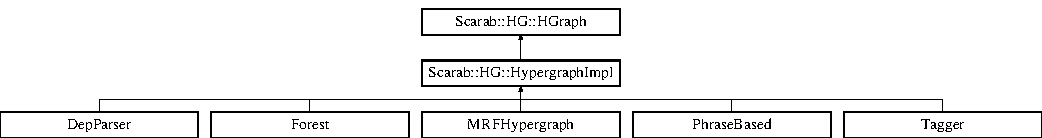
\includegraphics[height=1.85635cm]{classScarab_1_1HG_1_1HypergraphImpl}
\end{center}
\end{figure}
\subsection*{Public Member Functions}
\begin{DoxyCompactItemize}
\item 
\hypertarget{classScarab_1_1HG_1_1HypergraphImpl_a935bed9b8cf9235a1adb61d0889f6ac7}{
{\bfseries HypergraphImpl} (vector$<$ \hyperlink{classScarab_1_1HG_1_1Hypernode}{Hypernode} $\ast$ $>$ nodes, vector$<$ \hyperlink{classScarab_1_1HG_1_1Hyperedge}{Hyperedge} $\ast$ $>$ edges, \hyperlink{classScarab_1_1HG_1_1Hypernode}{Hypernode} $\ast$root)}
\label{classScarab_1_1HG_1_1HypergraphImpl_a935bed9b8cf9235a1adb61d0889f6ac7}

\item 
const \hyperlink{classScarab_1_1HG_1_1Hypernode}{Hypernode} \& \hyperlink{classScarab_1_1HG_1_1HypergraphImpl_a31172009b97d179f6b1199f191197a32}{root} () const 
\item 
\hypertarget{classScarab_1_1HG_1_1HypergraphImpl_a0adcc8783b94cbe07b092220082d00ab}{
unsigned int {\bfseries num\_\-edges} () const }
\label{classScarab_1_1HG_1_1HypergraphImpl_a0adcc8783b94cbe07b092220082d00ab}

\item 
\hypertarget{classScarab_1_1HG_1_1HypergraphImpl_ad39e917a84acb1d4caf0145ce8a903a2}{
uint {\bfseries num\_\-nodes} () const }
\label{classScarab_1_1HG_1_1HypergraphImpl_ad39e917a84acb1d4caf0145ce8a903a2}

\item 
\hypertarget{classScarab_1_1HG_1_1HypergraphImpl_a9276a6faa074eb4f3bbb2f8b8d5d4fbf}{
const \hyperlink{classScarab_1_1HG_1_1Hypernode}{Hypernode} \& {\bfseries get\_\-node} (unsigned int i) const }
\label{classScarab_1_1HG_1_1HypergraphImpl_a9276a6faa074eb4f3bbb2f8b8d5d4fbf}

\item 
\hypertarget{classScarab_1_1HG_1_1HypergraphImpl_a31a148139b888b6bd10e78fe555144c7}{
const \hyperlink{classScarab_1_1HG_1_1Hyperedge}{Hyperedge} \& {\bfseries get\_\-edge} (uint i) const }
\label{classScarab_1_1HG_1_1HypergraphImpl_a31a148139b888b6bd10e78fe555144c7}

\item 
\hypertarget{classScarab_1_1HG_1_1HypergraphImpl_a1f33418f90b826db9cfc0bb34e1ca9cf}{
void {\bfseries build\_\-from\_\-file} (const char $\ast$file\_\-name)}
\label{classScarab_1_1HG_1_1HypergraphImpl_a1f33418f90b826db9cfc0bb34e1ca9cf}

\item 
const vector$<$ \hyperlink{classScarab_1_1HG_1_1Hypernode}{Hypernode} $\ast$ $>$ \& \hyperlink{classScarab_1_1HG_1_1HypergraphImpl_a9aef2881b489c86d4d83e996a70f8141}{nodes} () const 
\item 
const vector$<$ \hyperlink{classScarab_1_1HG_1_1Hyperedge}{Hyperedge} $\ast$ $>$ \& \hyperlink{classScarab_1_1HG_1_1HypergraphImpl_a0c8373e545fe59b0cb7036b4751508e1}{edges} () const 
\item 
\hypertarget{classScarab_1_1HG_1_1HypergraphImpl_a98701d5529aaf3e5d4fa386694843f20}{
void {\bfseries prune} (const \hyperlink{structScarab_1_1HG_1_1HypergraphPrune}{HypergraphPrune} \&prune)}
\label{classScarab_1_1HG_1_1HypergraphImpl_a98701d5529aaf3e5d4fa386694843f20}

\item 
\hypertarget{classScarab_1_1HG_1_1HypergraphImpl_af8f5ed38a355676c473e8d54b5552cc6}{
void {\bfseries write\_\-to\_\-file} (const char $\ast$file\_\-name)}
\label{classScarab_1_1HG_1_1HypergraphImpl_af8f5ed38a355676c473e8d54b5552cc6}

\end{DoxyCompactItemize}
\subsection*{Protected Member Functions}
\begin{DoxyCompactItemize}
\item 
\hypertarget{classScarab_1_1HG_1_1HypergraphImpl_af14198ba5fccb5d4118188fa42feb8ff}{
virtual \hyperlink{classScarab_1_1HG_1_1Hypernode}{Hypernode} $\ast$ {\bfseries make\_\-node} (const \hyperlink{classHypergraph__Node}{Hypergraph\_\-Node} \&node, wvector $\ast$features)}
\label{classScarab_1_1HG_1_1HypergraphImpl_af14198ba5fccb5d4118188fa42feb8ff}

\item 
\hypertarget{classScarab_1_1HG_1_1HypergraphImpl_a238a7ce3b578c8126eccbc7803570638}{
virtual void {\bfseries make\_\-edge} (const \hyperlink{classHypergraph__Edge}{Hypergraph\_\-Edge} \&edge, const \hyperlink{classScarab_1_1HG_1_1Hyperedge}{Hyperedge} $\ast$our\_\-edge)}
\label{classScarab_1_1HG_1_1HypergraphImpl_a238a7ce3b578c8126eccbc7803570638}

\item 
\hypertarget{classScarab_1_1HG_1_1HypergraphImpl_a30349aca0e3b8f8dc72ed74d78e8c5b8}{
virtual void {\bfseries convert\_\-edge} (const \hyperlink{classScarab_1_1HG_1_1Hyperedge}{Hyperedge} $\ast$our\_\-edge, \hyperlink{classHypergraph__Edge}{Hypergraph\_\-Edge} $\ast$edge)}
\label{classScarab_1_1HG_1_1HypergraphImpl_a30349aca0e3b8f8dc72ed74d78e8c5b8}

\item 
\hypertarget{classScarab_1_1HG_1_1HypergraphImpl_a93e9e250fa457a2171bf07241b7829eb}{
virtual void {\bfseries convert\_\-node} (const \hyperlink{classScarab_1_1HG_1_1Hypernode}{Hypernode} $\ast$our\_\-node, \hyperlink{classHypergraph__Node}{Hypergraph\_\-Node} $\ast$node)}
\label{classScarab_1_1HG_1_1HypergraphImpl_a93e9e250fa457a2171bf07241b7829eb}

\item 
\hypertarget{classScarab_1_1HG_1_1HypergraphImpl_ae91de73e633e450b01664e3ec964019c}{
virtual void {\bfseries set\_\-up} (const \hyperlink{classHypergraph}{Hypergraph} \&hgraph)}
\label{classScarab_1_1HG_1_1HypergraphImpl_ae91de73e633e450b01664e3ec964019c}

\end{DoxyCompactItemize}
\subsection*{Protected Attributes}
\begin{DoxyCompactItemize}
\item 
\hypertarget{classScarab_1_1HG_1_1HypergraphImpl_aa7192cf8f168e5bfed67a8faf85c8cb4}{
::\hyperlink{classHypergraph}{Hypergraph} $\ast$ {\bfseries hgraph}}
\label{classScarab_1_1HG_1_1HypergraphImpl_aa7192cf8f168e5bfed67a8faf85c8cb4}

\item 
\hypertarget{classScarab_1_1HG_1_1HypergraphImpl_a7035fdae4c04d0752aaaf1e7eba7600e}{
\hyperlink{classScarab_1_1HG_1_1Hypernode}{Hypernode} $\ast$ {\bfseries \_\-root}}
\label{classScarab_1_1HG_1_1HypergraphImpl_a7035fdae4c04d0752aaaf1e7eba7600e}

\item 
\hypertarget{classScarab_1_1HG_1_1HypergraphImpl_a4cc57d9255e2f09714c5913d67cd0554}{
vector$<$ \hyperlink{classScarab_1_1HG_1_1Hypernode}{Hypernode} $\ast$ $>$ {\bfseries \_\-nodes}}
\label{classScarab_1_1HG_1_1HypergraphImpl_a4cc57d9255e2f09714c5913d67cd0554}

\item 
\hypertarget{classScarab_1_1HG_1_1HypergraphImpl_a56fb710140f3359646b1a17cb0417d74}{
vector$<$ \hyperlink{classScarab_1_1HG_1_1Hyperedge}{Hyperedge} $\ast$ $>$ {\bfseries \_\-edges}}
\label{classScarab_1_1HG_1_1HypergraphImpl_a56fb710140f3359646b1a17cb0417d74}

\end{DoxyCompactItemize}


\subsection{Member Function Documentation}
\hypertarget{classScarab_1_1HG_1_1HypergraphImpl_a0c8373e545fe59b0cb7036b4751508e1}{
\index{Scarab::HG::HypergraphImpl@{Scarab::HG::HypergraphImpl}!edges@{edges}}
\index{edges@{edges}!Scarab::HG::HypergraphImpl@{Scarab::HG::HypergraphImpl}}
\subsubsection[{edges}]{\setlength{\rightskip}{0pt plus 5cm}const vector$<${\bf Hyperedge}$\ast$$>$\& Scarab::HG::HypergraphImpl::edges () const\hspace{0.3cm}{\ttfamily  \mbox{[}inline, virtual\mbox{]}}}}
\label{classScarab_1_1HG_1_1HypergraphImpl_a0c8373e545fe59b0cb7036b4751508e1}
Get all hyperedges in the hypergraph. (Assume unordered) WARNING: Treat this as a const iterator. \begin{DoxyReturn}{Returns}
Const iterator to edges in hypergraph . 
\end{DoxyReturn}


Implements \hyperlink{classScarab_1_1HG_1_1HGraph_a57328729f90cc4152ca79ff15ecdd4bb}{Scarab::HG::HGraph}.

\hypertarget{classScarab_1_1HG_1_1HypergraphImpl_a9aef2881b489c86d4d83e996a70f8141}{
\index{Scarab::HG::HypergraphImpl@{Scarab::HG::HypergraphImpl}!nodes@{nodes}}
\index{nodes@{nodes}!Scarab::HG::HypergraphImpl@{Scarab::HG::HypergraphImpl}}
\subsubsection[{nodes}]{\setlength{\rightskip}{0pt plus 5cm}const vector$<${\bf Hypernode}$\ast$$>$\& Scarab::HG::HypergraphImpl::nodes () const\hspace{0.3cm}{\ttfamily  \mbox{[}inline, virtual\mbox{]}}}}
\label{classScarab_1_1HG_1_1HypergraphImpl_a9aef2881b489c86d4d83e996a70f8141}
Get all hypernodes in the hypergraph. (Assume unordered) WARNING: Treat this as a const iterator. \begin{DoxyReturn}{Returns}
Const iterator to hypernodes in hypergraph . 
\end{DoxyReturn}


Implements \hyperlink{classScarab_1_1HG_1_1HGraph_a74d893fba015520774f71f02a46bb6ca}{Scarab::HG::HGraph}.

\hypertarget{classScarab_1_1HG_1_1HypergraphImpl_a31172009b97d179f6b1199f191197a32}{
\index{Scarab::HG::HypergraphImpl@{Scarab::HG::HypergraphImpl}!root@{root}}
\index{root@{root}!Scarab::HG::HypergraphImpl@{Scarab::HG::HypergraphImpl}}
\subsubsection[{root}]{\setlength{\rightskip}{0pt plus 5cm}const {\bf Hypernode}\& Scarab::HG::HypergraphImpl::root () const\hspace{0.3cm}{\ttfamily  \mbox{[}inline, virtual\mbox{]}}}}
\label{classScarab_1_1HG_1_1HypergraphImpl_a31172009b97d179f6b1199f191197a32}
Get the root of the hypergraph

\begin{DoxyReturn}{Returns}
\hyperlink{classScarab_1_1HG_1_1Hypernode}{Hypernode} at root 
\end{DoxyReturn}


Implements \hyperlink{classScarab_1_1HG_1_1HGraph_a5ede392b158e41dd7e95ded1c4b0b5d6}{Scarab::HG::HGraph}.



The documentation for this class was generated from the following files:\begin{DoxyCompactItemize}
\item 
hypergraph/HypergraphImpl.h\item 
hypergraph/HypergraphImpl.cpp\end{DoxyCompactItemize}

\hypertarget{structScarab_1_1HG_1_1HypergraphLP}{
\section{Scarab::HG::HypergraphLP Struct Reference}
\label{structScarab_1_1HG_1_1HypergraphLP}\index{Scarab::HG::HypergraphLP@{Scarab::HG::HypergraphLP}}
}
\subsection*{Public Member Functions}
\begin{DoxyCompactItemize}
\item 
\hypertarget{structScarab_1_1HG_1_1HypergraphLP_a332edf79e5fc5b617ec6e948a73cc4a4}{
{\bfseries HypergraphLP} (const \hyperlink{classScarab_1_1HG_1_1HGraph}{HGraph} \&h)}
\label{structScarab_1_1HG_1_1HypergraphLP_a332edf79e5fc5b617ec6e948a73cc4a4}

\end{DoxyCompactItemize}
\subsection*{Public Attributes}
\begin{DoxyCompactItemize}
\item 
\hypertarget{structScarab_1_1HG_1_1HypergraphLP_ae9c9c441b112e98e412e8129e91a28ce}{
\hyperlink{classCache}{Cache}$<$ \hyperlink{classScarab_1_1HG_1_1Hypernode}{Hypernode}, GRBVar $>$ {\bfseries node\_\-vars}}
\label{structScarab_1_1HG_1_1HypergraphLP_ae9c9c441b112e98e412e8129e91a28ce}

\item 
\hypertarget{structScarab_1_1HG_1_1HypergraphLP_a8e71b062f3d6691eef27bb85c718604f}{
\hyperlink{classCache}{Cache}$<$ \hyperlink{classScarab_1_1HG_1_1Hyperedge}{Hyperedge}, GRBVar $>$ {\bfseries edge\_\-vars}}
\label{structScarab_1_1HG_1_1HypergraphLP_a8e71b062f3d6691eef27bb85c718604f}

\item 
\hypertarget{structScarab_1_1HG_1_1HypergraphLP_a52fa717afa9c902f7d8ef3adf18c5204}{
const \hyperlink{classScarab_1_1HG_1_1HGraph}{HGraph} \& {\bfseries \_\-h}}
\label{structScarab_1_1HG_1_1HypergraphLP_a52fa717afa9c902f7d8ef3adf18c5204}

\end{DoxyCompactItemize}


The documentation for this struct was generated from the following file:\begin{DoxyCompactItemize}
\item 
lp/HypergraphLP.h\end{DoxyCompactItemize}

\hypertarget{classScarab_1_1HG_1_1HypergraphLPBuilder}{
\section{Scarab::HG::HypergraphLPBuilder Class Reference}
\label{classScarab_1_1HG_1_1HypergraphLPBuilder}\index{Scarab::HG::HypergraphLPBuilder@{Scarab::HG::HypergraphLPBuilder}}
}
\subsection*{Static Public Member Functions}
\begin{DoxyCompactItemize}
\item 
\hypertarget{classScarab_1_1HG_1_1HypergraphLPBuilder_a7653a6f997f1505c0d6668618b28d6d8}{
static void {\bfseries show\_\-hypergraph} (const \hyperlink{structScarab_1_1HG_1_1HypergraphLP}{HypergraphLP} \&h\_\-lp)}
\label{classScarab_1_1HG_1_1HypergraphLPBuilder_a7653a6f997f1505c0d6668618b28d6d8}

\item 
\hypertarget{classScarab_1_1HG_1_1HypergraphLPBuilder_a3a711a79152e0f5d4cc9157737673b95}{
static \hyperlink{structScarab_1_1HG_1_1HypergraphLP}{HypergraphLP} $\ast$ {\bfseries add\_\-hypergraph} (const \hyperlink{classScarab_1_1HG_1_1HGraph}{HGraph} \&h, const \hyperlink{classCache}{Cache}$<$ \hyperlink{classScarab_1_1HG_1_1Hyperedge}{Hyperedge}, double $>$ \&\_\-weights, string prefix, GRBModel \&model, int var\_\-type)}
\label{classScarab_1_1HG_1_1HypergraphLPBuilder_a3a711a79152e0f5d4cc9157737673b95}

\end{DoxyCompactItemize}


The documentation for this class was generated from the following file:\begin{DoxyCompactItemize}
\item 
lp/HypergraphLP.h\end{DoxyCompactItemize}

\hypertarget{structScarab_1_1HG_1_1HypergraphPrune}{
\section{Scarab::HG::HypergraphPrune Struct Reference}
\label{structScarab_1_1HG_1_1HypergraphPrune}\index{Scarab::HG::HypergraphPrune@{Scarab::HG::HypergraphPrune}}
}
\subsection*{Public Member Functions}
\begin{DoxyCompactItemize}
\item 
\hypertarget{structScarab_1_1HG_1_1HypergraphPrune_adc29528f39ad9ced03be8b48341c3e84}{
{\bfseries HypergraphPrune} (const \hyperlink{classScarab_1_1HG_1_1HGraph}{HGraph} \&hgraph\_\-)}
\label{structScarab_1_1HG_1_1HypergraphPrune_adc29528f39ad9ced03be8b48341c3e84}

\end{DoxyCompactItemize}
\subsection*{Public Attributes}
\begin{DoxyCompactItemize}
\item 
\hypertarget{structScarab_1_1HG_1_1HypergraphPrune_a1ff0fd7b723f888db33ae542d186d0b4}{
set$<$ int $>$ {\bfseries nodes}}
\label{structScarab_1_1HG_1_1HypergraphPrune_a1ff0fd7b723f888db33ae542d186d0b4}

\item 
\hypertarget{structScarab_1_1HG_1_1HypergraphPrune_adff9a55407cd2cff9199d440ef513029}{
set$<$ int $>$ {\bfseries edges}}
\label{structScarab_1_1HG_1_1HypergraphPrune_adff9a55407cd2cff9199d440ef513029}

\item 
\hypertarget{structScarab_1_1HG_1_1HypergraphPrune_a55f12db438013ace2d307efb284bcb7b}{
const \hyperlink{classScarab_1_1HG_1_1HGraph}{HGraph} \& {\bfseries hgraph}}
\label{structScarab_1_1HG_1_1HypergraphPrune_a55f12db438013ace2d307efb284bcb7b}

\end{DoxyCompactItemize}


The documentation for this struct was generated from the following file:\begin{DoxyCompactItemize}
\item 
hypergraph/Hypergraph.h\end{DoxyCompactItemize}

\hypertarget{classHypergraphTools}{
\section{HypergraphTools Class Reference}
\label{classHypergraphTools}\index{HypergraphTools@{HypergraphTools}}
}
\subsection*{Public Member Functions}
\begin{DoxyCompactItemize}
\item 
\hypertarget{classHypergraphTools_a188643770705ed9482616956e22ebfd4}{
void {\bfseries viterbi} (HGraph g)}
\label{classHypergraphTools_a188643770705ed9482616956e22ebfd4}

\end{DoxyCompactItemize}


The documentation for this class was generated from the following file:\begin{DoxyCompactItemize}
\item 
hypergraph/HypergraphTools.h\end{DoxyCompactItemize}

\hypertarget{classScarab_1_1HG_1_1Hypernode}{
\section{Scarab::HG::Hypernode Class Reference}
\label{classScarab_1_1HG_1_1Hypernode}\index{Scarab::HG::Hypernode@{Scarab::HG::Hypernode}}
}


{\ttfamily \#include $<$Hypergraph.h$>$}

Inheritance diagram for Scarab::HG::Hypernode:\begin{figure}[H]
\begin{center}
\leavevmode
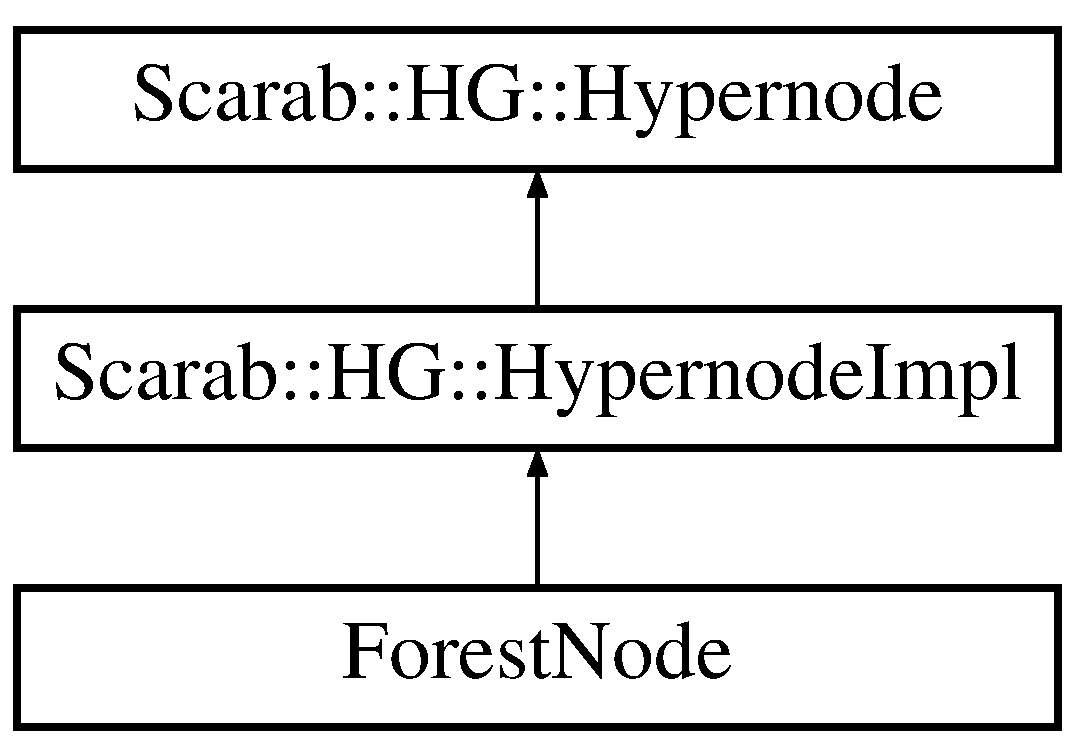
\includegraphics[height=3cm]{classScarab_1_1HG_1_1Hypernode}
\end{center}
\end{figure}
\subsection*{Public Member Functions}
\begin{DoxyCompactItemize}
\item 
virtual \hyperlink{classScarab_1_1HG_1_1Hypernode_a0657cc96f62d29da3ae4b5b9bcab1ce6}{$\sim$Hypernode} ()
\item 
virtual unsigned int \hyperlink{classScarab_1_1HG_1_1Hypernode_a0aeaee6c2ca2a011fcd086f803aaa4d0}{id} () const =0
\item 
virtual unsigned int \hyperlink{classScarab_1_1HG_1_1Hypernode_add2f4d556be223b906bfbab9f1b60870}{num\_\-edges} () const =0
\item 
virtual unsigned int \hyperlink{classScarab_1_1HG_1_1Hypernode_a4b1a4ffaa8a8b0295763673e6d86d693}{num\_\-in\_\-edges} () const =0
\item 
virtual const \hyperlink{classScarab_1_1HG_1_1Hyperedge}{Hyperedge} \& \hyperlink{classScarab_1_1HG_1_1Hypernode_a3bface6832eb54a00d90e4fe8d1999f7}{edge} (unsigned int i) const =0
\item 
virtual const \hyperlink{classScarab_1_1HG_1_1Hyperedge}{Hyperedge} \& \hyperlink{classScarab_1_1HG_1_1Hypernode_a533d3e0bc2269ec07edbda32305daf70}{in\_\-edge} (unsigned int i) const =0
\item 
virtual bool \hyperlink{classScarab_1_1HG_1_1Hypernode_ae3e1107309a8817d1015bd70a90c1c49}{is\_\-terminal} () const =0
\item 
virtual const vector$<$ \hyperlink{classScarab_1_1HG_1_1Hyperedge}{Hyperedge} $\ast$ $>$ \& \hyperlink{classScarab_1_1HG_1_1Hypernode_a3306572ded5b5061c1916bcf268be94e}{edges} () const =0
\item 
virtual const vector$<$ \hyperlink{classScarab_1_1HG_1_1Hyperedge}{Hyperedge} $\ast$ $>$ \& \hyperlink{classScarab_1_1HG_1_1Hypernode_aad118748408663b8242dc52d45bbd49d}{in\_\-edges} () const =0
\end{DoxyCompactItemize}


\subsection{Detailed Description}
\hyperlink{classScarab_1_1HG_1_1Hypernode}{Hypernode} -\/ Constant representation of a hypernode in a hypergraph. Accessors for edges above and below. 

\subsection{Constructor \& Destructor Documentation}
\hypertarget{classScarab_1_1HG_1_1Hypernode_a0657cc96f62d29da3ae4b5b9bcab1ce6}{
\index{Scarab::HG::Hypernode@{Scarab::HG::Hypernode}!$\sim$Hypernode@{$\sim$Hypernode}}
\index{$\sim$Hypernode@{$\sim$Hypernode}!Scarab::HG::Hypernode@{Scarab::HG::Hypernode}}
\subsubsection[{$\sim$Hypernode}]{\setlength{\rightskip}{0pt plus 5cm}virtual Scarab::HG::Hypernode::$\sim$Hypernode ()\hspace{0.3cm}{\ttfamily  \mbox{[}inline, virtual\mbox{]}}}}
\label{classScarab_1_1HG_1_1Hypernode_a0657cc96f62d29da3ae4b5b9bcab1ce6}
WARNING: Private except to \hyperlink{classHypergraph}{Hypergraph} 

\subsection{Member Function Documentation}
\hypertarget{classScarab_1_1HG_1_1Hypernode_a3bface6832eb54a00d90e4fe8d1999f7}{
\index{Scarab::HG::Hypernode@{Scarab::HG::Hypernode}!edge@{edge}}
\index{edge@{edge}!Scarab::HG::Hypernode@{Scarab::HG::Hypernode}}
\subsubsection[{edge}]{\setlength{\rightskip}{0pt plus 5cm}virtual const {\bf Hyperedge}\& Scarab::HG::Hypernode::edge (unsigned int {\em i}) const\hspace{0.3cm}{\ttfamily  \mbox{[}pure virtual\mbox{]}}}}
\label{classScarab_1_1HG_1_1Hypernode_a3bface6832eb54a00d90e4fe8d1999f7}
Get the hyperedge this node as head \begin{Desc}
\item[\hyperlink{deprecated__deprecated000009}{Deprecated}]\end{Desc}

\begin{DoxyParams}{Parameters}
\item[{\em i}]Local local id of edge\end{DoxyParams}
\begin{DoxyReturn}{Returns}
The hyperedge 
\end{DoxyReturn}


Implemented in \hyperlink{classScarab_1_1HG_1_1HypernodeImpl_a328189f28a4185d435035686a27592c2}{Scarab::HG::HypernodeImpl}.

\hypertarget{classScarab_1_1HG_1_1Hypernode_a3306572ded5b5061c1916bcf268be94e}{
\index{Scarab::HG::Hypernode@{Scarab::HG::Hypernode}!edges@{edges}}
\index{edges@{edges}!Scarab::HG::Hypernode@{Scarab::HG::Hypernode}}
\subsubsection[{edges}]{\setlength{\rightskip}{0pt plus 5cm}virtual const vector$<${\bf Hyperedge}$\ast$$>$\& Scarab::HG::Hypernode::edges () const\hspace{0.3cm}{\ttfamily  \mbox{[}pure virtual\mbox{]}}}}
\label{classScarab_1_1HG_1_1Hypernode_a3306572ded5b5061c1916bcf268be94e}
Get all hyperedges with this hypernode as head. WARNING: Treat this as a const iterator. \begin{DoxyReturn}{Returns}
Const iterator to edges. 
\end{DoxyReturn}


Implemented in \hyperlink{classScarab_1_1HG_1_1HypernodeImpl_ada979dcddc1bf0abf0fc2530d1ea8761}{Scarab::HG::HypernodeImpl}.

\hypertarget{classScarab_1_1HG_1_1Hypernode_a0aeaee6c2ca2a011fcd086f803aaa4d0}{
\index{Scarab::HG::Hypernode@{Scarab::HG::Hypernode}!id@{id}}
\index{id@{id}!Scarab::HG::Hypernode@{Scarab::HG::Hypernode}}
\subsubsection[{id}]{\setlength{\rightskip}{0pt plus 5cm}virtual unsigned int Scarab::HG::Hypernode::id () const\hspace{0.3cm}{\ttfamily  \mbox{[}pure virtual\mbox{]}}}}
\label{classScarab_1_1HG_1_1Hypernode_a0aeaee6c2ca2a011fcd086f803aaa4d0}
The unique identifier of the \hyperlink{classScarab_1_1HG_1_1Hypernode}{Hypernode} \begin{Desc}
\item[\hyperlink{deprecated__deprecated000006}{Deprecated}]\end{Desc}
\begin{DoxyReturn}{Returns}
The number 
\end{DoxyReturn}


Implemented in \hyperlink{classScarab_1_1HG_1_1HypernodeImpl_a2579ef1e67ad8f51d23838c130440d21}{Scarab::HG::HypernodeImpl}.

\hypertarget{classScarab_1_1HG_1_1Hypernode_a533d3e0bc2269ec07edbda32305daf70}{
\index{Scarab::HG::Hypernode@{Scarab::HG::Hypernode}!in\_\-edge@{in\_\-edge}}
\index{in\_\-edge@{in\_\-edge}!Scarab::HG::Hypernode@{Scarab::HG::Hypernode}}
\subsubsection[{in\_\-edge}]{\setlength{\rightskip}{0pt plus 5cm}virtual const {\bf Hyperedge}\& Scarab::HG::Hypernode::in\_\-edge (unsigned int {\em i}) const\hspace{0.3cm}{\ttfamily  \mbox{[}pure virtual\mbox{]}}}}
\label{classScarab_1_1HG_1_1Hypernode_a533d3e0bc2269ec07edbda32305daf70}
Get the hyperedge this node as tail \begin{Desc}
\item[\hyperlink{deprecated__deprecated000010}{Deprecated}]\end{Desc}

\begin{DoxyParams}{Parameters}
\item[{\em i}]Local local id of edge\end{DoxyParams}
\begin{DoxyReturn}{Returns}
The hyperedge 
\end{DoxyReturn}


Implemented in \hyperlink{classScarab_1_1HG_1_1HypernodeImpl_a26ff9db30c03c7b74181e9f901aa71d4}{Scarab::HG::HypernodeImpl}.

\hypertarget{classScarab_1_1HG_1_1Hypernode_aad118748408663b8242dc52d45bbd49d}{
\index{Scarab::HG::Hypernode@{Scarab::HG::Hypernode}!in\_\-edges@{in\_\-edges}}
\index{in\_\-edges@{in\_\-edges}!Scarab::HG::Hypernode@{Scarab::HG::Hypernode}}
\subsubsection[{in\_\-edges}]{\setlength{\rightskip}{0pt plus 5cm}virtual const vector$<${\bf Hyperedge}$\ast$$>$\& Scarab::HG::Hypernode::in\_\-edges () const\hspace{0.3cm}{\ttfamily  \mbox{[}pure virtual\mbox{]}}}}
\label{classScarab_1_1HG_1_1Hypernode_aad118748408663b8242dc52d45bbd49d}
Get all hyperedges with this hypernode as a tail. WARNING: Treat this as a const iterator. \begin{DoxyReturn}{Returns}
Const iterator to edges. 
\end{DoxyReturn}


Implemented in \hyperlink{classScarab_1_1HG_1_1HypernodeImpl_a77fe0de2e3927be6145cb8fc018088c9}{Scarab::HG::HypernodeImpl}.

\hypertarget{classScarab_1_1HG_1_1Hypernode_ae3e1107309a8817d1015bd70a90c1c49}{
\index{Scarab::HG::Hypernode@{Scarab::HG::Hypernode}!is\_\-terminal@{is\_\-terminal}}
\index{is\_\-terminal@{is\_\-terminal}!Scarab::HG::Hypernode@{Scarab::HG::Hypernode}}
\subsubsection[{is\_\-terminal}]{\setlength{\rightskip}{0pt plus 5cm}virtual bool Scarab::HG::Hypernode::is\_\-terminal () const\hspace{0.3cm}{\ttfamily  \mbox{[}pure virtual\mbox{]}}}}
\label{classScarab_1_1HG_1_1Hypernode_ae3e1107309a8817d1015bd70a90c1c49}
Is this node a terminal nodes. (no children)

\begin{DoxyReturn}{Returns}
True if terminal (assert \hyperlink{classScarab_1_1HG_1_1Hypernode_ae3e1107309a8817d1015bd70a90c1c49}{is\_\-terminal()} == (\hyperlink{classScarab_1_1HG_1_1Hypernode_add2f4d556be223b906bfbab9f1b60870}{num\_\-edges()} == 0)) 
\end{DoxyReturn}


Implemented in \hyperlink{classScarab_1_1HG_1_1HypernodeImpl_a2bb4b33ff207c3c1babe135b9af6323e}{Scarab::HG::HypernodeImpl}.

\hypertarget{classScarab_1_1HG_1_1Hypernode_add2f4d556be223b906bfbab9f1b60870}{
\index{Scarab::HG::Hypernode@{Scarab::HG::Hypernode}!num\_\-edges@{num\_\-edges}}
\index{num\_\-edges@{num\_\-edges}!Scarab::HG::Hypernode@{Scarab::HG::Hypernode}}
\subsubsection[{num\_\-edges}]{\setlength{\rightskip}{0pt plus 5cm}virtual unsigned int Scarab::HG::Hypernode::num\_\-edges () const\hspace{0.3cm}{\ttfamily  \mbox{[}pure virtual\mbox{]}}}}
\label{classScarab_1_1HG_1_1Hypernode_add2f4d556be223b906bfbab9f1b60870}
Get the number of hyperedges that have this node as head \begin{Desc}
\item[\hyperlink{deprecated__deprecated000007}{Deprecated}]\end{Desc}
\begin{DoxyReturn}{Returns}
The number 
\end{DoxyReturn}


Implemented in \hyperlink{classScarab_1_1HG_1_1HypernodeImpl_a7fed4809706319cc916ed4c04a641436}{Scarab::HG::HypernodeImpl}.

\hypertarget{classScarab_1_1HG_1_1Hypernode_a4b1a4ffaa8a8b0295763673e6d86d693}{
\index{Scarab::HG::Hypernode@{Scarab::HG::Hypernode}!num\_\-in\_\-edges@{num\_\-in\_\-edges}}
\index{num\_\-in\_\-edges@{num\_\-in\_\-edges}!Scarab::HG::Hypernode@{Scarab::HG::Hypernode}}
\subsubsection[{num\_\-in\_\-edges}]{\setlength{\rightskip}{0pt plus 5cm}virtual unsigned int Scarab::HG::Hypernode::num\_\-in\_\-edges () const\hspace{0.3cm}{\ttfamily  \mbox{[}pure virtual\mbox{]}}}}
\label{classScarab_1_1HG_1_1Hypernode_a4b1a4ffaa8a8b0295763673e6d86d693}
Get the number of hyperedges that have this node as tail \begin{Desc}
\item[\hyperlink{deprecated__deprecated000008}{Deprecated}]\end{Desc}
\begin{DoxyReturn}{Returns}
The number 
\end{DoxyReturn}


Implemented in \hyperlink{classScarab_1_1HG_1_1HypernodeImpl_a9a13a37fcece16603ec4bf3f364e6fcc}{Scarab::HG::HypernodeImpl}.



The documentation for this class was generated from the following file:\begin{DoxyCompactItemize}
\item 
hypergraph/Hypergraph.h\end{DoxyCompactItemize}

\hypertarget{classScarab_1_1HG_1_1HypernodeImpl}{
\section{Scarab::HG::HypernodeImpl Class Reference}
\label{classScarab_1_1HG_1_1HypernodeImpl}\index{Scarab::HG::HypernodeImpl@{Scarab::HG::HypernodeImpl}}
}
Inheritance diagram for Scarab::HG::HypernodeImpl:\begin{figure}[H]
\begin{center}
\leavevmode
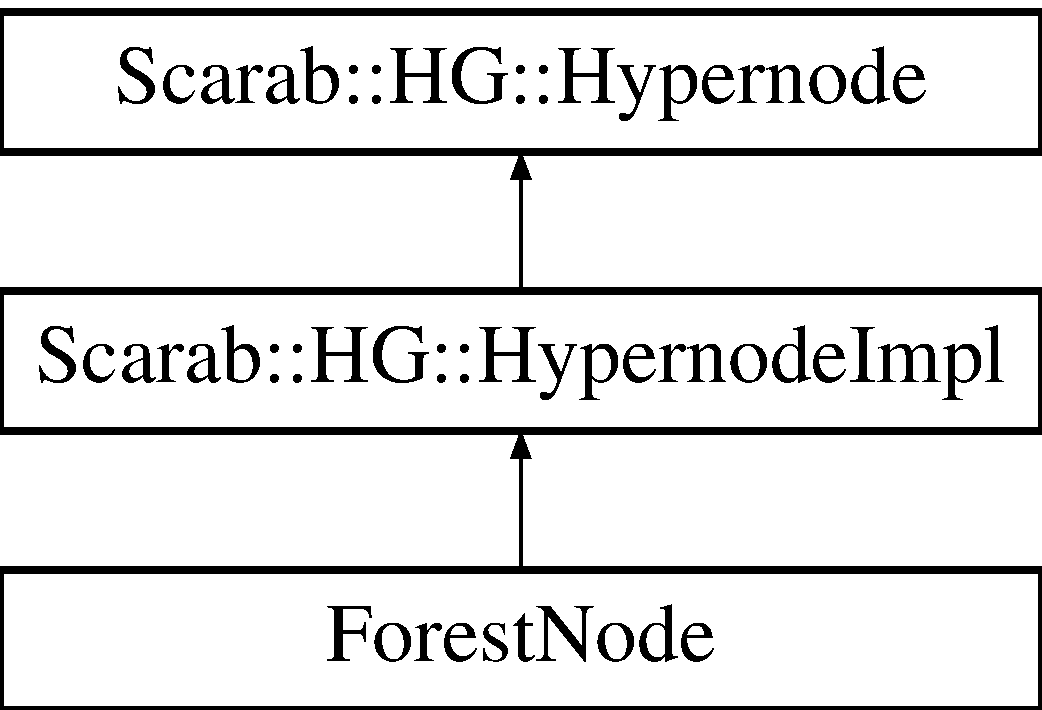
\includegraphics[height=3cm]{classScarab_1_1HG_1_1HypernodeImpl}
\end{center}
\end{figure}
\subsection*{Public Member Functions}
\begin{DoxyCompactItemize}
\item 
\hypertarget{classScarab_1_1HG_1_1HypernodeImpl_a574c6f1386fb27894075977ef1ca56d6}{
{\bfseries HypernodeImpl} (const string \&label, int id, \hyperlink{classsvector}{wvector} $\ast$features)}
\label{classScarab_1_1HG_1_1HypernodeImpl_a574c6f1386fb27894075977ef1ca56d6}

\item 
\hypertarget{classScarab_1_1HG_1_1HypernodeImpl_a0899a4e97f535c2f005d7c5ab5364681}{
void {\bfseries add\_\-edge} (\hyperlink{classScarab_1_1HG_1_1Hyperedge}{Hyperedge} $\ast$edge)}
\label{classScarab_1_1HG_1_1HypernodeImpl_a0899a4e97f535c2f005d7c5ab5364681}

\item 
\hypertarget{classScarab_1_1HG_1_1HypernodeImpl_ab05500702d5fa1c896efe941f9c54bf3}{
void {\bfseries add\_\-in\_\-edge} (\hyperlink{classScarab_1_1HG_1_1Hyperedge}{Hyperedge} $\ast$edge)}
\label{classScarab_1_1HG_1_1HypernodeImpl_ab05500702d5fa1c896efe941f9c54bf3}

\item 
bool \hyperlink{classScarab_1_1HG_1_1HypernodeImpl_a2bb4b33ff207c3c1babe135b9af6323e}{is\_\-terminal} () const 
\item 
\hypertarget{classScarab_1_1HG_1_1HypernodeImpl_a6675d677bd7e794ae9a8bf72645b828a}{
void {\bfseries prune\_\-edges} (const set$<$ int $>$ \&keep\_\-edges)}
\label{classScarab_1_1HG_1_1HypernodeImpl_a6675d677bd7e794ae9a8bf72645b828a}

\item 
const \hyperlink{classScarab_1_1HG_1_1Hyperedge}{Hyperedge} \& \hyperlink{classScarab_1_1HG_1_1HypernodeImpl_a328189f28a4185d435035686a27592c2}{edge} (uint i) const 
\item 
unsigned int \hyperlink{classScarab_1_1HG_1_1HypernodeImpl_a7fed4809706319cc916ed4c04a641436}{num\_\-edges} () const 
\item 
unsigned int \hyperlink{classScarab_1_1HG_1_1HypernodeImpl_a9a13a37fcece16603ec4bf3f364e6fcc}{num\_\-in\_\-edges} () const 
\item 
const \hyperlink{classScarab_1_1HG_1_1Hyperedge}{Hyperedge} \& \hyperlink{classScarab_1_1HG_1_1HypernodeImpl_a26ff9db30c03c7b74181e9f901aa71d4}{in\_\-edge} (uint i) const 
\item 
uint \hyperlink{classScarab_1_1HG_1_1HypernodeImpl_a2579ef1e67ad8f51d23838c130440d21}{id} () const 
\item 
const vector$<$ \hyperlink{classScarab_1_1HG_1_1Hyperedge}{Hyperedge} $\ast$ $>$ \& \hyperlink{classScarab_1_1HG_1_1HypernodeImpl_ada979dcddc1bf0abf0fc2530d1ea8761}{edges} () const 
\item 
const vector$<$ \hyperlink{classScarab_1_1HG_1_1Hyperedge}{Hyperedge} $\ast$ $>$ \& \hyperlink{classScarab_1_1HG_1_1HypernodeImpl_a77fe0de2e3927be6145cb8fc018088c9}{in\_\-edges} () const 
\item 
\hypertarget{classScarab_1_1HG_1_1HypernodeImpl_a9b0df10dfd6c20c094a928f1ced76f90}{
void {\bfseries reid} (int new\_\-id)}
\label{classScarab_1_1HG_1_1HypernodeImpl_a9b0df10dfd6c20c094a928f1ced76f90}

\end{DoxyCompactItemize}
\subsection*{Public Attributes}
\begin{DoxyCompactItemize}
\item 
\hypertarget{classScarab_1_1HG_1_1HypernodeImpl_aaa189784dcf714f3c1ca54ea8cd0dc83}{
vector$<$ \hyperlink{classScarab_1_1HG_1_1Hyperedge}{Hyperedge} $\ast$ $>$ {\bfseries \_\-edges}}
\label{classScarab_1_1HG_1_1HypernodeImpl_aaa189784dcf714f3c1ca54ea8cd0dc83}

\item 
\hypertarget{classScarab_1_1HG_1_1HypernodeImpl_aefb3b14843d6fb8ed2284ae0d6a53dbd}{
const string \& {\bfseries \_\-label}}
\label{classScarab_1_1HG_1_1HypernodeImpl_aefb3b14843d6fb8ed2284ae0d6a53dbd}

\end{DoxyCompactItemize}


\subsection{Member Function Documentation}
\hypertarget{classScarab_1_1HG_1_1HypernodeImpl_a328189f28a4185d435035686a27592c2}{
\index{Scarab::HG::HypernodeImpl@{Scarab::HG::HypernodeImpl}!edge@{edge}}
\index{edge@{edge}!Scarab::HG::HypernodeImpl@{Scarab::HG::HypernodeImpl}}
\subsubsection[{edge}]{\setlength{\rightskip}{0pt plus 5cm}const {\bf Hyperedge}\& Scarab::HG::HypernodeImpl::edge (uint {\em i}) const\hspace{0.3cm}{\ttfamily  \mbox{[}inline, virtual\mbox{]}}}}
\label{classScarab_1_1HG_1_1HypernodeImpl_a328189f28a4185d435035686a27592c2}
Get the hyperedge this node as head \begin{Desc}
\item[\hyperlink{deprecated__deprecated000009}{Deprecated}]\end{Desc}

\begin{DoxyParams}{Parameters}
\item[{\em i}]Local local id of edge\end{DoxyParams}
\begin{DoxyReturn}{Returns}
The hyperedge 
\end{DoxyReturn}


Implements \hyperlink{classScarab_1_1HG_1_1Hypernode_a3bface6832eb54a00d90e4fe8d1999f7}{Scarab::HG::Hypernode}.

\hypertarget{classScarab_1_1HG_1_1HypernodeImpl_ada979dcddc1bf0abf0fc2530d1ea8761}{
\index{Scarab::HG::HypernodeImpl@{Scarab::HG::HypernodeImpl}!edges@{edges}}
\index{edges@{edges}!Scarab::HG::HypernodeImpl@{Scarab::HG::HypernodeImpl}}
\subsubsection[{edges}]{\setlength{\rightskip}{0pt plus 5cm}const vector$<${\bf Hyperedge}$\ast$$>$\& Scarab::HG::HypernodeImpl::edges () const\hspace{0.3cm}{\ttfamily  \mbox{[}inline, virtual\mbox{]}}}}
\label{classScarab_1_1HG_1_1HypernodeImpl_ada979dcddc1bf0abf0fc2530d1ea8761}
Get all hyperedges with this hypernode as head. WARNING: Treat this as a const iterator. \begin{DoxyReturn}{Returns}
Const iterator to edges. 
\end{DoxyReturn}


Implements \hyperlink{classScarab_1_1HG_1_1Hypernode_a3306572ded5b5061c1916bcf268be94e}{Scarab::HG::Hypernode}.

\hypertarget{classScarab_1_1HG_1_1HypernodeImpl_a2579ef1e67ad8f51d23838c130440d21}{
\index{Scarab::HG::HypernodeImpl@{Scarab::HG::HypernodeImpl}!id@{id}}
\index{id@{id}!Scarab::HG::HypernodeImpl@{Scarab::HG::HypernodeImpl}}
\subsubsection[{id}]{\setlength{\rightskip}{0pt plus 5cm}uint Scarab::HG::HypernodeImpl::id () const\hspace{0.3cm}{\ttfamily  \mbox{[}inline, virtual\mbox{]}}}}
\label{classScarab_1_1HG_1_1HypernodeImpl_a2579ef1e67ad8f51d23838c130440d21}
The unique identifier of the \hyperlink{classScarab_1_1HG_1_1Hypernode}{Hypernode} \begin{Desc}
\item[\hyperlink{deprecated__deprecated000006}{Deprecated}]\end{Desc}
\begin{DoxyReturn}{Returns}
The number 
\end{DoxyReturn}


Implements \hyperlink{classScarab_1_1HG_1_1Hypernode_a0aeaee6c2ca2a011fcd086f803aaa4d0}{Scarab::HG::Hypernode}.

\hypertarget{classScarab_1_1HG_1_1HypernodeImpl_a26ff9db30c03c7b74181e9f901aa71d4}{
\index{Scarab::HG::HypernodeImpl@{Scarab::HG::HypernodeImpl}!in\_\-edge@{in\_\-edge}}
\index{in\_\-edge@{in\_\-edge}!Scarab::HG::HypernodeImpl@{Scarab::HG::HypernodeImpl}}
\subsubsection[{in\_\-edge}]{\setlength{\rightskip}{0pt plus 5cm}const {\bf Hyperedge}\& Scarab::HG::HypernodeImpl::in\_\-edge (uint {\em i}) const\hspace{0.3cm}{\ttfamily  \mbox{[}inline, virtual\mbox{]}}}}
\label{classScarab_1_1HG_1_1HypernodeImpl_a26ff9db30c03c7b74181e9f901aa71d4}
Get the hyperedge this node as tail \begin{Desc}
\item[\hyperlink{deprecated__deprecated000010}{Deprecated}]\end{Desc}

\begin{DoxyParams}{Parameters}
\item[{\em i}]Local local id of edge\end{DoxyParams}
\begin{DoxyReturn}{Returns}
The hyperedge 
\end{DoxyReturn}


Implements \hyperlink{classScarab_1_1HG_1_1Hypernode_a533d3e0bc2269ec07edbda32305daf70}{Scarab::HG::Hypernode}.

\hypertarget{classScarab_1_1HG_1_1HypernodeImpl_a77fe0de2e3927be6145cb8fc018088c9}{
\index{Scarab::HG::HypernodeImpl@{Scarab::HG::HypernodeImpl}!in\_\-edges@{in\_\-edges}}
\index{in\_\-edges@{in\_\-edges}!Scarab::HG::HypernodeImpl@{Scarab::HG::HypernodeImpl}}
\subsubsection[{in\_\-edges}]{\setlength{\rightskip}{0pt plus 5cm}const vector$<${\bf Hyperedge}$\ast$$>$\& Scarab::HG::HypernodeImpl::in\_\-edges () const\hspace{0.3cm}{\ttfamily  \mbox{[}inline, virtual\mbox{]}}}}
\label{classScarab_1_1HG_1_1HypernodeImpl_a77fe0de2e3927be6145cb8fc018088c9}
Get all hyperedges with this hypernode as a tail. WARNING: Treat this as a const iterator. \begin{DoxyReturn}{Returns}
Const iterator to edges. 
\end{DoxyReturn}


Implements \hyperlink{classScarab_1_1HG_1_1Hypernode_aad118748408663b8242dc52d45bbd49d}{Scarab::HG::Hypernode}.

\hypertarget{classScarab_1_1HG_1_1HypernodeImpl_a2bb4b33ff207c3c1babe135b9af6323e}{
\index{Scarab::HG::HypernodeImpl@{Scarab::HG::HypernodeImpl}!is\_\-terminal@{is\_\-terminal}}
\index{is\_\-terminal@{is\_\-terminal}!Scarab::HG::HypernodeImpl@{Scarab::HG::HypernodeImpl}}
\subsubsection[{is\_\-terminal}]{\setlength{\rightskip}{0pt plus 5cm}bool Scarab::HG::HypernodeImpl::is\_\-terminal () const\hspace{0.3cm}{\ttfamily  \mbox{[}inline, virtual\mbox{]}}}}
\label{classScarab_1_1HG_1_1HypernodeImpl_a2bb4b33ff207c3c1babe135b9af6323e}
Is this node a terminal nodes. (no children)

\begin{DoxyReturn}{Returns}
True if terminal (assert \hyperlink{classScarab_1_1HG_1_1HypernodeImpl_a2bb4b33ff207c3c1babe135b9af6323e}{is\_\-terminal()} == (\hyperlink{classScarab_1_1HG_1_1HypernodeImpl_a7fed4809706319cc916ed4c04a641436}{num\_\-edges()} == 0)) 
\end{DoxyReturn}


Implements \hyperlink{classScarab_1_1HG_1_1Hypernode_ae3e1107309a8817d1015bd70a90c1c49}{Scarab::HG::Hypernode}.

\hypertarget{classScarab_1_1HG_1_1HypernodeImpl_a7fed4809706319cc916ed4c04a641436}{
\index{Scarab::HG::HypernodeImpl@{Scarab::HG::HypernodeImpl}!num\_\-edges@{num\_\-edges}}
\index{num\_\-edges@{num\_\-edges}!Scarab::HG::HypernodeImpl@{Scarab::HG::HypernodeImpl}}
\subsubsection[{num\_\-edges}]{\setlength{\rightskip}{0pt plus 5cm}unsigned int Scarab::HG::HypernodeImpl::num\_\-edges () const\hspace{0.3cm}{\ttfamily  \mbox{[}inline, virtual\mbox{]}}}}
\label{classScarab_1_1HG_1_1HypernodeImpl_a7fed4809706319cc916ed4c04a641436}
Get the number of hyperedges that have this node as head \begin{Desc}
\item[\hyperlink{deprecated__deprecated000007}{Deprecated}]\end{Desc}
\begin{DoxyReturn}{Returns}
The number 
\end{DoxyReturn}


Implements \hyperlink{classScarab_1_1HG_1_1Hypernode_add2f4d556be223b906bfbab9f1b60870}{Scarab::HG::Hypernode}.

\hypertarget{classScarab_1_1HG_1_1HypernodeImpl_a9a13a37fcece16603ec4bf3f364e6fcc}{
\index{Scarab::HG::HypernodeImpl@{Scarab::HG::HypernodeImpl}!num\_\-in\_\-edges@{num\_\-in\_\-edges}}
\index{num\_\-in\_\-edges@{num\_\-in\_\-edges}!Scarab::HG::HypernodeImpl@{Scarab::HG::HypernodeImpl}}
\subsubsection[{num\_\-in\_\-edges}]{\setlength{\rightskip}{0pt plus 5cm}unsigned int Scarab::HG::HypernodeImpl::num\_\-in\_\-edges () const\hspace{0.3cm}{\ttfamily  \mbox{[}inline, virtual\mbox{]}}}}
\label{classScarab_1_1HG_1_1HypernodeImpl_a9a13a37fcece16603ec4bf3f364e6fcc}
Get the number of hyperedges that have this node as tail \begin{Desc}
\item[\hyperlink{deprecated__deprecated000008}{Deprecated}]\end{Desc}
\begin{DoxyReturn}{Returns}
The number 
\end{DoxyReturn}


Implements \hyperlink{classScarab_1_1HG_1_1Hypernode_a4b1a4ffaa8a8b0295763673e6d86d693}{Scarab::HG::Hypernode}.



The documentation for this class was generated from the following file:\begin{DoxyCompactItemize}
\item 
hypergraph/HypergraphImpl.h\end{DoxyCompactItemize}

\hypertarget{structScarab_1_1HG_1_1Hypothesis}{
\section{Scarab::HG::Hypothesis Struct Reference}
\label{structScarab_1_1HG_1_1Hypothesis}\index{Scarab::HG::Hypothesis@{Scarab::HG::Hypothesis}}
}
\subsection*{Public Member Functions}
\begin{DoxyCompactItemize}
\item 
\hyperlink{structScarab_1_1HG_1_1Hypothesis_aca7357ce485cb960fadb2cc62f1a888a}{Hypothesis} (const \hyperlink{structScarab_1_1HG_1_1State}{State} \&left\_\-hook, const \hyperlink{structScarab_1_1HG_1_1State}{State} \&right, \hyperlink{classScarab_1_1HG_1_1Hyperedge}{HEdge} back\_\-pointer)
\item 
\hypertarget{structScarab_1_1HG_1_1Hypothesis_a0d71b86d0d7d3294e61671efed2722bf}{
{\bfseries Hypothesis} (const \hyperlink{structScarab_1_1HG_1_1State}{State} \&left\_\-hook, const \hyperlink{structScarab_1_1HG_1_1State}{State} \&right)}
\label{structScarab_1_1HG_1_1Hypothesis_a0d71b86d0d7d3294e61671efed2722bf}

\item 
\hypertarget{structScarab_1_1HG_1_1Hypothesis_a974fd973dd0c8a380f342bbd10013d6f}{
{\bfseries Hypothesis} (int d)}
\label{structScarab_1_1HG_1_1Hypothesis_a974fd973dd0c8a380f342bbd10013d6f}

\item 
bool \hyperlink{structScarab_1_1HG_1_1Hypothesis_a698008183fc3863a0c03ba0c3e5960d1}{match} (const \hyperlink{structScarab_1_1HG_1_1Hypothesis}{Hypothesis} \&other) const 
\item 
int \hyperlink{structScarab_1_1HG_1_1Hypothesis_a5a69f417c889d4d96ad5a78aa1dd2f7d}{id} () const 
\item 
int \hyperlink{structScarab_1_1HG_1_1Hypothesis_ac428cffa80bad102222f58463bfba7e5}{left} () const 
\item 
int \hyperlink{structScarab_1_1HG_1_1Hypothesis_a6c026d211fd4f4875216fc179a78e879}{right} () const 
\item 
\hypertarget{structScarab_1_1HG_1_1Hypothesis_a70597628ead54cb83fcda7422d6d2f1f}{
bool {\bfseries operator$<$} (const \hyperlink{structScarab_1_1HG_1_1Hypothesis}{Hypothesis} \&other) const }
\label{structScarab_1_1HG_1_1Hypothesis_a70597628ead54cb83fcda7422d6d2f1f}

\end{DoxyCompactItemize}
\subsection*{Public Attributes}
\begin{DoxyCompactItemize}
\item 
\hypertarget{structScarab_1_1HG_1_1Hypothesis_a53277642394df6145ea8bfc6a3e3996e}{
\hyperlink{structScarab_1_1HG_1_1State}{State} {\bfseries hook}}
\label{structScarab_1_1HG_1_1Hypothesis_a53277642394df6145ea8bfc6a3e3996e}

\item 
\hypertarget{structScarab_1_1HG_1_1Hypothesis_aff1779905d4f7e9a21b71a20cec4f02d}{
\hyperlink{structScarab_1_1HG_1_1State}{State} {\bfseries right\_\-side}}
\label{structScarab_1_1HG_1_1Hypothesis_aff1779905d4f7e9a21b71a20cec4f02d}

\item 
\hypertarget{structScarab_1_1HG_1_1Hypothesis_aa31a2d052ecaffa034d8447de748946f}{
const \hyperlink{classScarab_1_1HG_1_1Hyperedge}{Hyperedge} $\ast$ {\bfseries back\_\-edge}}
\label{structScarab_1_1HG_1_1Hypothesis_aa31a2d052ecaffa034d8447de748946f}

\item 
\hypertarget{structScarab_1_1HG_1_1Hypothesis_a38b1068d18fe3ce28d6c93e5d12b2225}{
bool {\bfseries is\_\-done}}
\label{structScarab_1_1HG_1_1Hypothesis_a38b1068d18fe3ce28d6c93e5d12b2225}

\item 
\hypertarget{structScarab_1_1HG_1_1Hypothesis_a93bf33767cecd362e8a12d385c94be1a}{
vector$<$ int $>$ {\bfseries prev\_\-hyp}}
\label{structScarab_1_1HG_1_1Hypothesis_a93bf33767cecd362e8a12d385c94be1a}

\item 
\hypertarget{structScarab_1_1HG_1_1Hypothesis_a95df46740f1263062f4898db1b39cd41}{
double {\bfseries original\_\-value}}
\label{structScarab_1_1HG_1_1Hypothesis_a95df46740f1263062f4898db1b39cd41}

\end{DoxyCompactItemize}
\subsection*{Friends}
\begin{DoxyCompactItemize}
\item 
\hypertarget{structScarab_1_1HG_1_1Hypothesis_a70fdb92646880290a9c906e5018c11bb}{
ostream \& {\bfseries operator$<$$<$} (ostream \&output, const \hyperlink{structScarab_1_1HG_1_1Hypothesis}{Hypothesis} \&h)}
\label{structScarab_1_1HG_1_1Hypothesis_a70fdb92646880290a9c906e5018c11bb}

\end{DoxyCompactItemize}


\subsection{Constructor \& Destructor Documentation}
\hypertarget{structScarab_1_1HG_1_1Hypothesis_aca7357ce485cb960fadb2cc62f1a888a}{
\index{Scarab::HG::Hypothesis@{Scarab::HG::Hypothesis}!Hypothesis@{Hypothesis}}
\index{Hypothesis@{Hypothesis}!Scarab::HG::Hypothesis@{Scarab::HG::Hypothesis}}
\subsubsection[{Hypothesis}]{\setlength{\rightskip}{0pt plus 5cm}Scarab::HG::Hypothesis::Hypothesis (const {\bf State} \& {\em left\_\-hook}, \/  const {\bf State} \& {\em right}, \/  {\bf HEdge} {\em back\_\-pointer})\hspace{0.3cm}{\ttfamily  \mbox{[}inline\mbox{]}}}}
\label{structScarab_1_1HG_1_1Hypothesis_aca7357ce485cb960fadb2cc62f1a888a}
A \hyperlink{structScarab_1_1HG_1_1Hypothesis}{Hypothesis} represents the path through an intersection of a hypergraph and finite state automata.


\begin{DoxyParams}{Parameters}
\item[{\em left\_\-hook}]The expected fsa state on the left hand side \item[{\em right}]The current fsa state on the right hand side \item[{\em back\_\-pointer}]The last hyperedge taken on the path\end{DoxyParams}
\begin{DoxyReturn}{Returns}

\end{DoxyReturn}


\subsection{Member Function Documentation}
\hypertarget{structScarab_1_1HG_1_1Hypothesis_a5a69f417c889d4d96ad5a78aa1dd2f7d}{
\index{Scarab::HG::Hypothesis@{Scarab::HG::Hypothesis}!id@{id}}
\index{id@{id}!Scarab::HG::Hypothesis@{Scarab::HG::Hypothesis}}
\subsubsection[{id}]{\setlength{\rightskip}{0pt plus 5cm}int Scarab::HG::Hypothesis::id () const\hspace{0.3cm}{\ttfamily  \mbox{[}inline\mbox{]}}}}
\label{structScarab_1_1HG_1_1Hypothesis_a5a69f417c889d4d96ad5a78aa1dd2f7d}
Get the unique identifier for this hypothesis.

\begin{DoxyReturn}{Returns}

\end{DoxyReturn}
\hypertarget{structScarab_1_1HG_1_1Hypothesis_ac428cffa80bad102222f58463bfba7e5}{
\index{Scarab::HG::Hypothesis@{Scarab::HG::Hypothesis}!left@{left}}
\index{left@{left}!Scarab::HG::Hypothesis@{Scarab::HG::Hypothesis}}
\subsubsection[{left}]{\setlength{\rightskip}{0pt plus 5cm}int Scarab::HG::Hypothesis::left () const\hspace{0.3cm}{\ttfamily  \mbox{[}inline\mbox{]}}}}
\label{structScarab_1_1HG_1_1Hypothesis_ac428cffa80bad102222f58463bfba7e5}
Get the unique identifier for the left state of the hypothesis.

\begin{DoxyReturn}{Returns}
Left side id 
\end{DoxyReturn}
\hypertarget{structScarab_1_1HG_1_1Hypothesis_a698008183fc3863a0c03ba0c3e5960d1}{
\index{Scarab::HG::Hypothesis@{Scarab::HG::Hypothesis}!match@{match}}
\index{match@{match}!Scarab::HG::Hypothesis@{Scarab::HG::Hypothesis}}
\subsubsection[{match}]{\setlength{\rightskip}{0pt plus 5cm}bool Scarab::HG::Hypothesis::match (const {\bf Hypothesis} \& {\em other}) const\hspace{0.3cm}{\ttfamily  \mbox{[}inline\mbox{]}}}}
\label{structScarab_1_1HG_1_1Hypothesis_a698008183fc3863a0c03ba0c3e5960d1}
Is it valid to combine this hypothesis with another (do the fsa states match up) 
\begin{DoxyParams}{Parameters}
\item[{\em other}]The hypothesis to join on the right\end{DoxyParams}
\begin{DoxyReturn}{Returns}
True, if they match 
\end{DoxyReturn}
\hypertarget{structScarab_1_1HG_1_1Hypothesis_a6c026d211fd4f4875216fc179a78e879}{
\index{Scarab::HG::Hypothesis@{Scarab::HG::Hypothesis}!right@{right}}
\index{right@{right}!Scarab::HG::Hypothesis@{Scarab::HG::Hypothesis}}
\subsubsection[{right}]{\setlength{\rightskip}{0pt plus 5cm}int Scarab::HG::Hypothesis::right () const\hspace{0.3cm}{\ttfamily  \mbox{[}inline\mbox{]}}}}
\label{structScarab_1_1HG_1_1Hypothesis_a6c026d211fd4f4875216fc179a78e879}
Get the unique identifier for the right state of the hypothesis.

\begin{DoxyReturn}{Returns}
Right side id 
\end{DoxyReturn}


The documentation for this struct was generated from the following file:\begin{DoxyCompactItemize}
\item 
hypergraph/Hypothesis.h\end{DoxyCompactItemize}

\hypertarget{classlattice_1_1Lattice}{
\section{lattice::Lattice Class Reference}
\label{classlattice_1_1Lattice}\index{lattice::Lattice@{lattice::Lattice}}
}
\subsection*{Public Types}
\begin{DoxyCompactItemize}
\item 
\hypertarget{classlattice_1_1Lattice_a74f989d4c34d5ad1717a194194eaed71}{
typedef \hyperlink{classlattice_1_1Lattice__Node}{Lattice\_\-Node} {\bfseries Node}}
\label{classlattice_1_1Lattice_a74f989d4c34d5ad1717a194194eaed71}

\item 
\hypertarget{classlattice_1_1Lattice_a9f4acdebf1d889ee76d432dc549ee9b8}{
typedef \hyperlink{classlattice_1_1Lattice__Edge}{Lattice\_\-Edge} {\bfseries Edge}}
\label{classlattice_1_1Lattice_a9f4acdebf1d889ee76d432dc549ee9b8}

\end{DoxyCompactItemize}
\subsection*{Public Member Functions}
\begin{DoxyCompactItemize}
\item 
\hypertarget{classlattice_1_1Lattice_a6afe3eb36c5fa648ee09ff3425544a9f}{
{\bfseries Lattice} (const \hyperlink{classlattice_1_1Lattice}{Lattice} \&from)}
\label{classlattice_1_1Lattice_a6afe3eb36c5fa648ee09ff3425544a9f}

\item 
\hypertarget{classlattice_1_1Lattice_aaa4fc56dd3fca09222c685f78e2c5632}{
\hyperlink{classlattice_1_1Lattice}{Lattice} \& {\bfseries operator=} (const \hyperlink{classlattice_1_1Lattice}{Lattice} \&from)}
\label{classlattice_1_1Lattice_aaa4fc56dd3fca09222c685f78e2c5632}

\item 
\hypertarget{classlattice_1_1Lattice_afc9d0408a25d079574a8da841f4d2580}{
const ::google::protobuf::UnknownFieldSet \& {\bfseries unknown\_\-fields} () const }
\label{classlattice_1_1Lattice_afc9d0408a25d079574a8da841f4d2580}

\item 
\hypertarget{classlattice_1_1Lattice_a5581cb64b246c378c56bb2d686e42132}{
inline::google::protobuf::UnknownFieldSet $\ast$ {\bfseries mutable\_\-unknown\_\-fields} ()}
\label{classlattice_1_1Lattice_a5581cb64b246c378c56bb2d686e42132}

\item 
\hypertarget{classlattice_1_1Lattice_ab4a3958ab2281dfb4677e6b7998b5ff3}{
void {\bfseries Swap} (\hyperlink{classlattice_1_1Lattice}{Lattice} $\ast$other)}
\label{classlattice_1_1Lattice_ab4a3958ab2281dfb4677e6b7998b5ff3}

\item 
\hypertarget{classlattice_1_1Lattice_a947785986676e868ef33b975e406c14b}{
\hyperlink{classlattice_1_1Lattice}{Lattice} $\ast$ {\bfseries New} () const }
\label{classlattice_1_1Lattice_a947785986676e868ef33b975e406c14b}

\item 
\hypertarget{classlattice_1_1Lattice_a9aec9f61f02b520348f5b4e661f779ac}{
void {\bfseries CopyFrom} (const ::google::protobuf::Message \&from)}
\label{classlattice_1_1Lattice_a9aec9f61f02b520348f5b4e661f779ac}

\item 
\hypertarget{classlattice_1_1Lattice_a62644d01e4c7fc503661a3ac7a4461aa}{
void {\bfseries MergeFrom} (const ::google::protobuf::Message \&from)}
\label{classlattice_1_1Lattice_a62644d01e4c7fc503661a3ac7a4461aa}

\item 
\hypertarget{classlattice_1_1Lattice_a06293cf4a975500085cb11ff59418655}{
void {\bfseries CopyFrom} (const \hyperlink{classlattice_1_1Lattice}{Lattice} \&from)}
\label{classlattice_1_1Lattice_a06293cf4a975500085cb11ff59418655}

\item 
\hypertarget{classlattice_1_1Lattice_afcab65a875a55ec9f5ebc88f2b22a662}{
void {\bfseries MergeFrom} (const \hyperlink{classlattice_1_1Lattice}{Lattice} \&from)}
\label{classlattice_1_1Lattice_afcab65a875a55ec9f5ebc88f2b22a662}

\item 
\hypertarget{classlattice_1_1Lattice_a69643c6d759f3c59ca72f0b640e744cf}{
void {\bfseries Clear} ()}
\label{classlattice_1_1Lattice_a69643c6d759f3c59ca72f0b640e744cf}

\item 
\hypertarget{classlattice_1_1Lattice_a2a517e87a5ff555951149bd6c8f2fcc0}{
bool {\bfseries IsInitialized} () const }
\label{classlattice_1_1Lattice_a2a517e87a5ff555951149bd6c8f2fcc0}

\item 
\hypertarget{classlattice_1_1Lattice_aa1fa86cdd3f0897665f5a69c299ce120}{
int {\bfseries ByteSize} () const }
\label{classlattice_1_1Lattice_aa1fa86cdd3f0897665f5a69c299ce120}

\item 
\hypertarget{classlattice_1_1Lattice_a13776f9114d9135033c6a7ef0e5aa855}{
bool {\bfseries MergePartialFromCodedStream} (::google::protobuf::io::CodedInputStream $\ast$input)}
\label{classlattice_1_1Lattice_a13776f9114d9135033c6a7ef0e5aa855}

\item 
\hypertarget{classlattice_1_1Lattice_a211943e304584090a05bff477ba64bf3}{
void {\bfseries SerializeWithCachedSizes} (::google::protobuf::io::CodedOutputStream $\ast$output) const }
\label{classlattice_1_1Lattice_a211943e304584090a05bff477ba64bf3}

\item 
\hypertarget{classlattice_1_1Lattice_a679d526d9a589eb74f642d876fb5b339}{
::google::protobuf::uint8 $\ast$ {\bfseries SerializeWithCachedSizesToArray} (::google::protobuf::uint8 $\ast$output) const }
\label{classlattice_1_1Lattice_a679d526d9a589eb74f642d876fb5b339}

\item 
\hypertarget{classlattice_1_1Lattice_a93bab06ef91469b47be8794cacd5a5f7}{
int {\bfseries GetCachedSize} () const }
\label{classlattice_1_1Lattice_a93bab06ef91469b47be8794cacd5a5f7}

\item 
\hypertarget{classlattice_1_1Lattice_aaab0cda217c0772d69348f65cd35c33e}{
::google::protobuf::Metadata {\bfseries GetMetadata} () const }
\label{classlattice_1_1Lattice_aaab0cda217c0772d69348f65cd35c33e}

\item 
\hypertarget{classlattice_1_1Lattice_a3a06d03c8fc2d4810946301eb851d9bd}{
bool {\bfseries has\_\-start} () const }
\label{classlattice_1_1Lattice_a3a06d03c8fc2d4810946301eb851d9bd}

\item 
\hypertarget{classlattice_1_1Lattice_a8a22bdebf8702ccd1d7221acdd9447f9}{
void {\bfseries clear\_\-start} ()}
\label{classlattice_1_1Lattice_a8a22bdebf8702ccd1d7221acdd9447f9}

\item 
\hypertarget{classlattice_1_1Lattice_aa736b2c11a852db4859bb421de1b9d5b}{
inline::google::protobuf::int32 {\bfseries start} () const }
\label{classlattice_1_1Lattice_aa736b2c11a852db4859bb421de1b9d5b}

\item 
\hypertarget{classlattice_1_1Lattice_aeff8a9022b4341221a2fb81c0da4958c}{
void {\bfseries set\_\-start} (::google::protobuf::int32 value)}
\label{classlattice_1_1Lattice_aeff8a9022b4341221a2fb81c0da4958c}

\item 
\hypertarget{classlattice_1_1Lattice_acce3e8812b8edc5fee61a1c07144e35c}{
int {\bfseries final\_\-size} () const }
\label{classlattice_1_1Lattice_acce3e8812b8edc5fee61a1c07144e35c}

\item 
\hypertarget{classlattice_1_1Lattice_a796495494bd3460afe3a3da75d9a9866}{
void {\bfseries clear\_\-final} ()}
\label{classlattice_1_1Lattice_a796495494bd3460afe3a3da75d9a9866}

\item 
\hypertarget{classlattice_1_1Lattice_a047eb8b2fdf3ba5b0f34b175084d4957}{
inline::google::protobuf::int32 {\bfseries final} (int index) const }
\label{classlattice_1_1Lattice_a047eb8b2fdf3ba5b0f34b175084d4957}

\item 
\hypertarget{classlattice_1_1Lattice_afd8033a01d6390099a2a25033e38302f}{
void {\bfseries set\_\-final} (int index,::google::protobuf::int32 value)}
\label{classlattice_1_1Lattice_afd8033a01d6390099a2a25033e38302f}

\item 
\hypertarget{classlattice_1_1Lattice_a8b9c4979ec846fb10419fd0a776e2bf6}{
void {\bfseries add\_\-final} (::google::protobuf::int32 value)}
\label{classlattice_1_1Lattice_a8b9c4979ec846fb10419fd0a776e2bf6}

\item 
\hypertarget{classlattice_1_1Lattice_a2625e8a95bb6bc92ba4a4fb2ac54eea3}{
const ::google::protobuf::RepeatedField$<$ ::google::protobuf::int32 $>$ \& {\bfseries final} () const }
\label{classlattice_1_1Lattice_a2625e8a95bb6bc92ba4a4fb2ac54eea3}

\item 
\hypertarget{classlattice_1_1Lattice_a67607f04271c09637e771736078ab8b3}{
inline::google::protobuf::RepeatedField$<$ ::google::protobuf::int32 $>$ $\ast$ {\bfseries mutable\_\-final} ()}
\label{classlattice_1_1Lattice_a67607f04271c09637e771736078ab8b3}

\item 
\hypertarget{classlattice_1_1Lattice_ac6bb945f03a05b0e6fa66a5cdb17b854}{
int {\bfseries node\_\-size} () const }
\label{classlattice_1_1Lattice_ac6bb945f03a05b0e6fa66a5cdb17b854}

\item 
\hypertarget{classlattice_1_1Lattice_a21e99bbb5d73a80f4b3e79f053880b8f}{
void {\bfseries clear\_\-node} ()}
\label{classlattice_1_1Lattice_a21e99bbb5d73a80f4b3e79f053880b8f}

\item 
\hypertarget{classlattice_1_1Lattice_a388ba232d3051c050c645c4c5c49d8f0}{
const ::\hyperlink{classlattice_1_1Lattice__Node}{lattice::Lattice\_\-Node} \& {\bfseries node} (int index) const }
\label{classlattice_1_1Lattice_a388ba232d3051c050c645c4c5c49d8f0}

\item 
\hypertarget{classlattice_1_1Lattice_a80fd09af5dc4f602e3744ca984c55a57}{
inline::lattice::Lattice\_\-Node $\ast$ {\bfseries mutable\_\-node} (int index)}
\label{classlattice_1_1Lattice_a80fd09af5dc4f602e3744ca984c55a57}

\item 
\hypertarget{classlattice_1_1Lattice_abca614b554f335e8ea3c7a8950648113}{
inline::lattice::Lattice\_\-Node $\ast$ {\bfseries add\_\-node} ()}
\label{classlattice_1_1Lattice_abca614b554f335e8ea3c7a8950648113}

\item 
\hypertarget{classlattice_1_1Lattice_a76ff012c0dca5d00c46275522327852c}{
const ::google::protobuf::RepeatedPtrField$<$ ::\hyperlink{classlattice_1_1Lattice__Node}{lattice::Lattice\_\-Node} $>$ \& {\bfseries node} () const }
\label{classlattice_1_1Lattice_a76ff012c0dca5d00c46275522327852c}

\item 
\hypertarget{classlattice_1_1Lattice_ad1e861068dce2238dc2405442d40afa0}{
inline::google::protobuf::RepeatedPtrField$<$ ::\hyperlink{classlattice_1_1Lattice__Node}{lattice::Lattice\_\-Node} $>$ $\ast$ {\bfseries mutable\_\-node} ()}
\label{classlattice_1_1Lattice_ad1e861068dce2238dc2405442d40afa0}

\end{DoxyCompactItemize}
\subsection*{Static Public Member Functions}
\begin{DoxyCompactItemize}
\item 
\hypertarget{classlattice_1_1Lattice_a1439fffc17a145ba6bede8f9c693989e}{
static const ::google::protobuf::Descriptor $\ast$ {\bfseries descriptor} ()}
\label{classlattice_1_1Lattice_a1439fffc17a145ba6bede8f9c693989e}

\item 
\hypertarget{classlattice_1_1Lattice_ad46beb148ef5b77a4653a17ab5eff0b8}{
static const \hyperlink{classlattice_1_1Lattice}{Lattice} \& {\bfseries default\_\-instance} ()}
\label{classlattice_1_1Lattice_ad46beb148ef5b77a4653a17ab5eff0b8}

\end{DoxyCompactItemize}
\subsection*{Static Public Attributes}
\begin{DoxyCompactItemize}
\item 
\hypertarget{classlattice_1_1Lattice_a43c82461b5757da3dec815f9a1918546}{
static const int {\bfseries kStartFieldNumber} = 5}
\label{classlattice_1_1Lattice_a43c82461b5757da3dec815f9a1918546}

\item 
\hypertarget{classlattice_1_1Lattice_a41954f413ffb07063a80fb779f7b825b}{
static const int {\bfseries kFinalFieldNumber} = 6}
\label{classlattice_1_1Lattice_a41954f413ffb07063a80fb779f7b825b}

\item 
\hypertarget{classlattice_1_1Lattice_aef2900e37da8f683285328c24b5e6b16}{
static const int {\bfseries kNodeFieldNumber} = 7}
\label{classlattice_1_1Lattice_aef2900e37da8f683285328c24b5e6b16}

\end{DoxyCompactItemize}
\subsection*{Friends}
\begin{DoxyCompactItemize}
\item 
\hypertarget{classlattice_1_1Lattice_a19e63fb37025879e023cad88064187cf}{
void {\bfseries protobuf\_\-AddDesc\_\-lattice\_\-2eproto} ()}
\label{classlattice_1_1Lattice_a19e63fb37025879e023cad88064187cf}

\item 
\hypertarget{classlattice_1_1Lattice_a3b0386e09a9fefcf1bdce658cfc480b2}{
void {\bfseries protobuf\_\-AssignDesc\_\-lattice\_\-2eproto} ()}
\label{classlattice_1_1Lattice_a3b0386e09a9fefcf1bdce658cfc480b2}

\item 
\hypertarget{classlattice_1_1Lattice_a3c7b187721d0704ceb19ff889729d35a}{
void {\bfseries protobuf\_\-ShutdownFile\_\-lattice\_\-2eproto} ()}
\label{classlattice_1_1Lattice_a3c7b187721d0704ceb19ff889729d35a}

\end{DoxyCompactItemize}


The documentation for this class was generated from the following files:\begin{DoxyCompactItemize}
\item 
interfaces/lattice/gen-\/cpp/lattice.pb.h\item 
interfaces/lattice/gen-\/cpp/lattice.pb.cc\end{DoxyCompactItemize}

\hypertarget{classlattice_1_1Lattice__Edge}{
\section{lattice::Lattice\_\-Edge Class Reference}
\label{classlattice_1_1Lattice__Edge}\index{lattice::Lattice\_\-Edge@{lattice::Lattice\_\-Edge}}
}
\subsection*{Public Member Functions}
\begin{DoxyCompactItemize}
\item 
\hypertarget{classlattice_1_1Lattice__Edge_acd52c069d2b4ccd5e35415ced12a8de3}{
{\bfseries Lattice\_\-Edge} (const \hyperlink{classlattice_1_1Lattice__Edge}{Lattice\_\-Edge} \&from)}
\label{classlattice_1_1Lattice__Edge_acd52c069d2b4ccd5e35415ced12a8de3}

\item 
\hypertarget{classlattice_1_1Lattice__Edge_a7b8481bf7bbecf282e2f938ff35da177}{
\hyperlink{classlattice_1_1Lattice__Edge}{Lattice\_\-Edge} \& {\bfseries operator=} (const \hyperlink{classlattice_1_1Lattice__Edge}{Lattice\_\-Edge} \&from)}
\label{classlattice_1_1Lattice__Edge_a7b8481bf7bbecf282e2f938ff35da177}

\item 
\hypertarget{classlattice_1_1Lattice__Edge_af44f15fd53ae86dd482f86e74bf4ce55}{
const ::google::protobuf::UnknownFieldSet \& {\bfseries unknown\_\-fields} () const }
\label{classlattice_1_1Lattice__Edge_af44f15fd53ae86dd482f86e74bf4ce55}

\item 
\hypertarget{classlattice_1_1Lattice__Edge_aae27de06c0aa0d1cdae07ba720e7eb7c}{
inline::google::protobuf::UnknownFieldSet $\ast$ {\bfseries mutable\_\-unknown\_\-fields} ()}
\label{classlattice_1_1Lattice__Edge_aae27de06c0aa0d1cdae07ba720e7eb7c}

\item 
\hypertarget{classlattice_1_1Lattice__Edge_aaaa95dd26cb8b36f35652fba54be5679}{
void {\bfseries Swap} (\hyperlink{classlattice_1_1Lattice__Edge}{Lattice\_\-Edge} $\ast$other)}
\label{classlattice_1_1Lattice__Edge_aaaa95dd26cb8b36f35652fba54be5679}

\item 
\hypertarget{classlattice_1_1Lattice__Edge_a499e153dc35d1496be7a0420c5f848f3}{
\hyperlink{classlattice_1_1Lattice__Edge}{Lattice\_\-Edge} $\ast$ {\bfseries New} () const }
\label{classlattice_1_1Lattice__Edge_a499e153dc35d1496be7a0420c5f848f3}

\item 
\hypertarget{classlattice_1_1Lattice__Edge_a4f12ea2d09f06458eaf599bbd6140d09}{
void {\bfseries CopyFrom} (const ::google::protobuf::Message \&from)}
\label{classlattice_1_1Lattice__Edge_a4f12ea2d09f06458eaf599bbd6140d09}

\item 
\hypertarget{classlattice_1_1Lattice__Edge_acb2a52debadf89e32673ed4681a785de}{
void {\bfseries MergeFrom} (const ::google::protobuf::Message \&from)}
\label{classlattice_1_1Lattice__Edge_acb2a52debadf89e32673ed4681a785de}

\item 
\hypertarget{classlattice_1_1Lattice__Edge_a6a8426745b646d96dbea6931daaa33f9}{
void {\bfseries CopyFrom} (const \hyperlink{classlattice_1_1Lattice__Edge}{Lattice\_\-Edge} \&from)}
\label{classlattice_1_1Lattice__Edge_a6a8426745b646d96dbea6931daaa33f9}

\item 
\hypertarget{classlattice_1_1Lattice__Edge_ad910840c5215e942e5fad4b9119a4094}{
void {\bfseries MergeFrom} (const \hyperlink{classlattice_1_1Lattice__Edge}{Lattice\_\-Edge} \&from)}
\label{classlattice_1_1Lattice__Edge_ad910840c5215e942e5fad4b9119a4094}

\item 
\hypertarget{classlattice_1_1Lattice__Edge_a7780ee7c3441cce937784a92dda3fcad}{
void {\bfseries Clear} ()}
\label{classlattice_1_1Lattice__Edge_a7780ee7c3441cce937784a92dda3fcad}

\item 
\hypertarget{classlattice_1_1Lattice__Edge_a2a52f5e8c864ae50e31f7e0a5b5ece95}{
bool {\bfseries IsInitialized} () const }
\label{classlattice_1_1Lattice__Edge_a2a52f5e8c864ae50e31f7e0a5b5ece95}

\item 
\hypertarget{classlattice_1_1Lattice__Edge_a7342ae6a37ed9b432cdd4bacb58956b8}{
int {\bfseries ByteSize} () const }
\label{classlattice_1_1Lattice__Edge_a7342ae6a37ed9b432cdd4bacb58956b8}

\item 
\hypertarget{classlattice_1_1Lattice__Edge_ab3f9dc6f28a5d5e7356beb27f6cbdf3f}{
bool {\bfseries MergePartialFromCodedStream} (::google::protobuf::io::CodedInputStream $\ast$input)}
\label{classlattice_1_1Lattice__Edge_ab3f9dc6f28a5d5e7356beb27f6cbdf3f}

\item 
\hypertarget{classlattice_1_1Lattice__Edge_aa425ac46616eb3cbdc3e17b5536991c0}{
void {\bfseries SerializeWithCachedSizes} (::google::protobuf::io::CodedOutputStream $\ast$output) const }
\label{classlattice_1_1Lattice__Edge_aa425ac46616eb3cbdc3e17b5536991c0}

\item 
\hypertarget{classlattice_1_1Lattice__Edge_ab3717991484977072e673eaaaf28b9b5}{
::google::protobuf::uint8 $\ast$ {\bfseries SerializeWithCachedSizesToArray} (::google::protobuf::uint8 $\ast$output) const }
\label{classlattice_1_1Lattice__Edge_ab3717991484977072e673eaaaf28b9b5}

\item 
\hypertarget{classlattice_1_1Lattice__Edge_a6cccad4c342b1d0bf48b9b828f277b56}{
int {\bfseries GetCachedSize} () const }
\label{classlattice_1_1Lattice__Edge_a6cccad4c342b1d0bf48b9b828f277b56}

\item 
\hypertarget{classlattice_1_1Lattice__Edge_aba8500dcfc46ede1ae99f43ec1c5909f}{
::google::protobuf::Metadata {\bfseries GetMetadata} () const }
\label{classlattice_1_1Lattice__Edge_aba8500dcfc46ede1ae99f43ec1c5909f}

\item 
\hypertarget{classlattice_1_1Lattice__Edge_a8366be45d3f24bd44724f8ddabd5e3ac}{
bool {\bfseries has\_\-id} () const }
\label{classlattice_1_1Lattice__Edge_a8366be45d3f24bd44724f8ddabd5e3ac}

\item 
\hypertarget{classlattice_1_1Lattice__Edge_aa90e4552c9da9e7c3a62bff5af76540a}{
void {\bfseries clear\_\-id} ()}
\label{classlattice_1_1Lattice__Edge_aa90e4552c9da9e7c3a62bff5af76540a}

\item 
\hypertarget{classlattice_1_1Lattice__Edge_a99bb9339bff6dc5dea68711b5ea4739f}{
inline::google::protobuf::int32 {\bfseries id} () const }
\label{classlattice_1_1Lattice__Edge_a99bb9339bff6dc5dea68711b5ea4739f}

\item 
\hypertarget{classlattice_1_1Lattice__Edge_a24547494991007daed07e9526fe563a9}{
void {\bfseries set\_\-id} (::google::protobuf::int32 value)}
\label{classlattice_1_1Lattice__Edge_a24547494991007daed07e9526fe563a9}

\item 
\hypertarget{classlattice_1_1Lattice__Edge_ad835d581cf9d59feb757d7669b331813}{
bool {\bfseries has\_\-label} () const }
\label{classlattice_1_1Lattice__Edge_ad835d581cf9d59feb757d7669b331813}

\item 
\hypertarget{classlattice_1_1Lattice__Edge_a53d5c95032840aabb15521b04cf4343f}{
void {\bfseries clear\_\-label} ()}
\label{classlattice_1_1Lattice__Edge_a53d5c95032840aabb15521b04cf4343f}

\item 
\hypertarget{classlattice_1_1Lattice__Edge_a1bf88081324cb64246bd4b07b60010bf}{
const ::std::string \& {\bfseries label} () const }
\label{classlattice_1_1Lattice__Edge_a1bf88081324cb64246bd4b07b60010bf}

\item 
\hypertarget{classlattice_1_1Lattice__Edge_aec8f4c4697ebba26377929c894a2dba4}{
void {\bfseries set\_\-label} (const ::std::string \&value)}
\label{classlattice_1_1Lattice__Edge_aec8f4c4697ebba26377929c894a2dba4}

\item 
\hypertarget{classlattice_1_1Lattice__Edge_aa5056c3b346d89c79626bd9b76aaeda9}{
void {\bfseries set\_\-label} (const char $\ast$value)}
\label{classlattice_1_1Lattice__Edge_aa5056c3b346d89c79626bd9b76aaeda9}

\item 
\hypertarget{classlattice_1_1Lattice__Edge_afb812d783f60810acaff1f3cd5ede45e}{
void {\bfseries set\_\-label} (const char $\ast$value, size\_\-t size)}
\label{classlattice_1_1Lattice__Edge_afb812d783f60810acaff1f3cd5ede45e}

\item 
\hypertarget{classlattice_1_1Lattice__Edge_a422f058978331e9032f8b46f3e7edf19}{
inline::std::string $\ast$ {\bfseries mutable\_\-label} ()}
\label{classlattice_1_1Lattice__Edge_a422f058978331e9032f8b46f3e7edf19}

\item 
\hypertarget{classlattice_1_1Lattice__Edge_a19a5d69b5f49534574ba4228c2eabb00}{
inline::std::string $\ast$ {\bfseries release\_\-label} ()}
\label{classlattice_1_1Lattice__Edge_a19a5d69b5f49534574ba4228c2eabb00}

\item 
\hypertarget{classlattice_1_1Lattice__Edge_a8606af1eb69fe1603701acd62f1641fb}{
bool {\bfseries has\_\-to\_\-id} () const }
\label{classlattice_1_1Lattice__Edge_a8606af1eb69fe1603701acd62f1641fb}

\item 
\hypertarget{classlattice_1_1Lattice__Edge_a9b924c9c24c68d721caf410388ecd26b}{
void {\bfseries clear\_\-to\_\-id} ()}
\label{classlattice_1_1Lattice__Edge_a9b924c9c24c68d721caf410388ecd26b}

\item 
\hypertarget{classlattice_1_1Lattice__Edge_a15a7dd3d4bfd721431c5d40d2b775117}{
inline::google::protobuf::int32 {\bfseries to\_\-id} () const }
\label{classlattice_1_1Lattice__Edge_a15a7dd3d4bfd721431c5d40d2b775117}

\item 
\hypertarget{classlattice_1_1Lattice__Edge_afe2ba54700b6c255be550d5fddf03cea}{
void {\bfseries set\_\-to\_\-id} (::google::protobuf::int32 value)}
\label{classlattice_1_1Lattice__Edge_afe2ba54700b6c255be550d5fddf03cea}

\end{DoxyCompactItemize}
\subsection*{Static Public Member Functions}
\begin{DoxyCompactItemize}
\item 
\hypertarget{classlattice_1_1Lattice__Edge_a65852986232fb6963efbbc6fefd896be}{
static const ::google::protobuf::Descriptor $\ast$ {\bfseries descriptor} ()}
\label{classlattice_1_1Lattice__Edge_a65852986232fb6963efbbc6fefd896be}

\item 
\hypertarget{classlattice_1_1Lattice__Edge_ad6eb7c57bf5d859752e7e88bd7329469}{
static const \hyperlink{classlattice_1_1Lattice__Edge}{Lattice\_\-Edge} \& {\bfseries default\_\-instance} ()}
\label{classlattice_1_1Lattice__Edge_ad6eb7c57bf5d859752e7e88bd7329469}

\end{DoxyCompactItemize}
\subsection*{Static Public Attributes}
\begin{DoxyCompactItemize}
\item 
\hypertarget{classlattice_1_1Lattice__Edge_a0e2f2cee5173639eda89756b70265596}{
static const int {\bfseries kIdFieldNumber} = 1}
\label{classlattice_1_1Lattice__Edge_a0e2f2cee5173639eda89756b70265596}

\item 
\hypertarget{classlattice_1_1Lattice__Edge_a5c0b87e3bc9390f398cf3e2de0c19ca0}{
static const int {\bfseries kLabelFieldNumber} = 2}
\label{classlattice_1_1Lattice__Edge_a5c0b87e3bc9390f398cf3e2de0c19ca0}

\item 
\hypertarget{classlattice_1_1Lattice__Edge_a3bf87977ee5b7e5f33486c382fbac72f}{
static const int {\bfseries kToIdFieldNumber} = 3}
\label{classlattice_1_1Lattice__Edge_a3bf87977ee5b7e5f33486c382fbac72f}

\end{DoxyCompactItemize}
\subsection*{Friends}
\begin{DoxyCompactItemize}
\item 
\hypertarget{classlattice_1_1Lattice__Edge_a19e63fb37025879e023cad88064187cf}{
void {\bfseries protobuf\_\-AddDesc\_\-lattice\_\-2eproto} ()}
\label{classlattice_1_1Lattice__Edge_a19e63fb37025879e023cad88064187cf}

\item 
\hypertarget{classlattice_1_1Lattice__Edge_a3b0386e09a9fefcf1bdce658cfc480b2}{
void {\bfseries protobuf\_\-AssignDesc\_\-lattice\_\-2eproto} ()}
\label{classlattice_1_1Lattice__Edge_a3b0386e09a9fefcf1bdce658cfc480b2}

\item 
\hypertarget{classlattice_1_1Lattice__Edge_a3c7b187721d0704ceb19ff889729d35a}{
void {\bfseries protobuf\_\-ShutdownFile\_\-lattice\_\-2eproto} ()}
\label{classlattice_1_1Lattice__Edge_a3c7b187721d0704ceb19ff889729d35a}

\end{DoxyCompactItemize}


The documentation for this class was generated from the following files:\begin{DoxyCompactItemize}
\item 
interfaces/lattice/gen-\/cpp/lattice.pb.h\item 
interfaces/lattice/gen-\/cpp/lattice.pb.cc\end{DoxyCompactItemize}

\hypertarget{classlattice_1_1Lattice__Node}{
\section{lattice::Lattice\_\-Node Class Reference}
\label{classlattice_1_1Lattice__Node}\index{lattice::Lattice\_\-Node@{lattice::Lattice\_\-Node}}
}
\subsection*{Public Member Functions}
\begin{DoxyCompactItemize}
\item 
\hypertarget{classlattice_1_1Lattice__Node_a147424c31f0775202a79ceab4fa2fe8d}{
{\bfseries Lattice\_\-Node} (const \hyperlink{classlattice_1_1Lattice__Node}{Lattice\_\-Node} \&from)}
\label{classlattice_1_1Lattice__Node_a147424c31f0775202a79ceab4fa2fe8d}

\item 
\hypertarget{classlattice_1_1Lattice__Node_a27f953898aafca2d9fbd2622c4eeabbd}{
\hyperlink{classlattice_1_1Lattice__Node}{Lattice\_\-Node} \& {\bfseries operator=} (const \hyperlink{classlattice_1_1Lattice__Node}{Lattice\_\-Node} \&from)}
\label{classlattice_1_1Lattice__Node_a27f953898aafca2d9fbd2622c4eeabbd}

\item 
\hypertarget{classlattice_1_1Lattice__Node_a2f70b3b935aef09e0aee93a1e8a15561}{
const ::google::protobuf::UnknownFieldSet \& {\bfseries unknown\_\-fields} () const }
\label{classlattice_1_1Lattice__Node_a2f70b3b935aef09e0aee93a1e8a15561}

\item 
\hypertarget{classlattice_1_1Lattice__Node_a5c846fa08d1f88c39655400947f1c3cc}{
inline::google::protobuf::UnknownFieldSet $\ast$ {\bfseries mutable\_\-unknown\_\-fields} ()}
\label{classlattice_1_1Lattice__Node_a5c846fa08d1f88c39655400947f1c3cc}

\item 
\hypertarget{classlattice_1_1Lattice__Node_ab39220e03258bb1064634db1f021b0e3}{
void {\bfseries Swap} (\hyperlink{classlattice_1_1Lattice__Node}{Lattice\_\-Node} $\ast$other)}
\label{classlattice_1_1Lattice__Node_ab39220e03258bb1064634db1f021b0e3}

\item 
\hypertarget{classlattice_1_1Lattice__Node_a8c76bc3cfeef5b3e248f6a19906cce2e}{
\hyperlink{classlattice_1_1Lattice__Node}{Lattice\_\-Node} $\ast$ {\bfseries New} () const }
\label{classlattice_1_1Lattice__Node_a8c76bc3cfeef5b3e248f6a19906cce2e}

\item 
\hypertarget{classlattice_1_1Lattice__Node_a380df579ad1735c2126e4eba47e6f5e1}{
void {\bfseries CopyFrom} (const ::google::protobuf::Message \&from)}
\label{classlattice_1_1Lattice__Node_a380df579ad1735c2126e4eba47e6f5e1}

\item 
\hypertarget{classlattice_1_1Lattice__Node_a2fff3c85762dbffdb5f4db8a0d1f1de2}{
void {\bfseries MergeFrom} (const ::google::protobuf::Message \&from)}
\label{classlattice_1_1Lattice__Node_a2fff3c85762dbffdb5f4db8a0d1f1de2}

\item 
\hypertarget{classlattice_1_1Lattice__Node_a83833df54b108547003ddcd089e11495}{
void {\bfseries CopyFrom} (const \hyperlink{classlattice_1_1Lattice__Node}{Lattice\_\-Node} \&from)}
\label{classlattice_1_1Lattice__Node_a83833df54b108547003ddcd089e11495}

\item 
\hypertarget{classlattice_1_1Lattice__Node_a381edbfaee298b75d2326f7c2722a395}{
void {\bfseries MergeFrom} (const \hyperlink{classlattice_1_1Lattice__Node}{Lattice\_\-Node} \&from)}
\label{classlattice_1_1Lattice__Node_a381edbfaee298b75d2326f7c2722a395}

\item 
\hypertarget{classlattice_1_1Lattice__Node_a883603a4abfa63e055042e72c9a7d771}{
void {\bfseries Clear} ()}
\label{classlattice_1_1Lattice__Node_a883603a4abfa63e055042e72c9a7d771}

\item 
\hypertarget{classlattice_1_1Lattice__Node_a66f8bfa1d8df568cd212ecd39fc29e6c}{
bool {\bfseries IsInitialized} () const }
\label{classlattice_1_1Lattice__Node_a66f8bfa1d8df568cd212ecd39fc29e6c}

\item 
\hypertarget{classlattice_1_1Lattice__Node_a8af617033ad1ddf55c04869bf0eba7c8}{
int {\bfseries ByteSize} () const }
\label{classlattice_1_1Lattice__Node_a8af617033ad1ddf55c04869bf0eba7c8}

\item 
\hypertarget{classlattice_1_1Lattice__Node_a3d2d830c5d2004d848eefdb34ce4cd70}{
bool {\bfseries MergePartialFromCodedStream} (::google::protobuf::io::CodedInputStream $\ast$input)}
\label{classlattice_1_1Lattice__Node_a3d2d830c5d2004d848eefdb34ce4cd70}

\item 
\hypertarget{classlattice_1_1Lattice__Node_a9ba35eb712235a58d484d2f5d786664a}{
void {\bfseries SerializeWithCachedSizes} (::google::protobuf::io::CodedOutputStream $\ast$output) const }
\label{classlattice_1_1Lattice__Node_a9ba35eb712235a58d484d2f5d786664a}

\item 
\hypertarget{classlattice_1_1Lattice__Node_a97ca443a0cd91ec8a4f28f1d7e46e8d2}{
::google::protobuf::uint8 $\ast$ {\bfseries SerializeWithCachedSizesToArray} (::google::protobuf::uint8 $\ast$output) const }
\label{classlattice_1_1Lattice__Node_a97ca443a0cd91ec8a4f28f1d7e46e8d2}

\item 
\hypertarget{classlattice_1_1Lattice__Node_ad594e10f3cb4b49352ca4a851ef63103}{
int {\bfseries GetCachedSize} () const }
\label{classlattice_1_1Lattice__Node_ad594e10f3cb4b49352ca4a851ef63103}

\item 
\hypertarget{classlattice_1_1Lattice__Node_ab5abf471dae358e7a1819bbb4d16a8c9}{
::google::protobuf::Metadata {\bfseries GetMetadata} () const }
\label{classlattice_1_1Lattice__Node_ab5abf471dae358e7a1819bbb4d16a8c9}

\item 
\hypertarget{classlattice_1_1Lattice__Node_a527a11e30db84175ad17a4fe1d109434}{
bool {\bfseries has\_\-id} () const }
\label{classlattice_1_1Lattice__Node_a527a11e30db84175ad17a4fe1d109434}

\item 
\hypertarget{classlattice_1_1Lattice__Node_ab4a8aa29a8acc23ae517b3351466b4d4}{
void {\bfseries clear\_\-id} ()}
\label{classlattice_1_1Lattice__Node_ab4a8aa29a8acc23ae517b3351466b4d4}

\item 
\hypertarget{classlattice_1_1Lattice__Node_aa1365843c54d8275ff5ead668abe611e}{
inline::google::protobuf::int32 {\bfseries id} () const }
\label{classlattice_1_1Lattice__Node_aa1365843c54d8275ff5ead668abe611e}

\item 
\hypertarget{classlattice_1_1Lattice__Node_a64f4cd3b0fe45be92cd60ba160e6961b}{
void {\bfseries set\_\-id} (::google::protobuf::int32 value)}
\label{classlattice_1_1Lattice__Node_a64f4cd3b0fe45be92cd60ba160e6961b}

\item 
\hypertarget{classlattice_1_1Lattice__Node_ab785cdbb65eebc9069a36cf09f5ab4eb}{
bool {\bfseries has\_\-label} () const }
\label{classlattice_1_1Lattice__Node_ab785cdbb65eebc9069a36cf09f5ab4eb}

\item 
\hypertarget{classlattice_1_1Lattice__Node_a36a47fee6fb062d874140354e01bb5e4}{
void {\bfseries clear\_\-label} ()}
\label{classlattice_1_1Lattice__Node_a36a47fee6fb062d874140354e01bb5e4}

\item 
\hypertarget{classlattice_1_1Lattice__Node_a4baa3c21b2ea94a045439efcae5ed84f}{
const ::std::string \& {\bfseries label} () const }
\label{classlattice_1_1Lattice__Node_a4baa3c21b2ea94a045439efcae5ed84f}

\item 
\hypertarget{classlattice_1_1Lattice__Node_a154cd811d4bc7555f2a5d3ba945be6eb}{
void {\bfseries set\_\-label} (const ::std::string \&value)}
\label{classlattice_1_1Lattice__Node_a154cd811d4bc7555f2a5d3ba945be6eb}

\item 
\hypertarget{classlattice_1_1Lattice__Node_a4dea106b2814ec3e429f9d0cff796338}{
void {\bfseries set\_\-label} (const char $\ast$value)}
\label{classlattice_1_1Lattice__Node_a4dea106b2814ec3e429f9d0cff796338}

\item 
\hypertarget{classlattice_1_1Lattice__Node_a6a66a9b418f72c0687cf00ad75abf201}{
void {\bfseries set\_\-label} (const char $\ast$value, size\_\-t size)}
\label{classlattice_1_1Lattice__Node_a6a66a9b418f72c0687cf00ad75abf201}

\item 
\hypertarget{classlattice_1_1Lattice__Node_aa8755ed4cf007a1c8e781902fdc3a4f6}{
inline::std::string $\ast$ {\bfseries mutable\_\-label} ()}
\label{classlattice_1_1Lattice__Node_aa8755ed4cf007a1c8e781902fdc3a4f6}

\item 
\hypertarget{classlattice_1_1Lattice__Node_a48ddd3b16c87cd84a030e1106d9c44a8}{
inline::std::string $\ast$ {\bfseries release\_\-label} ()}
\label{classlattice_1_1Lattice__Node_a48ddd3b16c87cd84a030e1106d9c44a8}

\item 
\hypertarget{classlattice_1_1Lattice__Node_a0e92a26f2f5180cc98f1de7c6917b6d2}{
int {\bfseries edge\_\-size} () const }
\label{classlattice_1_1Lattice__Node_a0e92a26f2f5180cc98f1de7c6917b6d2}

\item 
\hypertarget{classlattice_1_1Lattice__Node_a09e1fc45aba7522fc5949bf7328947b1}{
void {\bfseries clear\_\-edge} ()}
\label{classlattice_1_1Lattice__Node_a09e1fc45aba7522fc5949bf7328947b1}

\item 
\hypertarget{classlattice_1_1Lattice__Node_a8c03817565b5fdbeec75b612358e9f9e}{
const ::\hyperlink{classlattice_1_1Lattice__Edge}{lattice::Lattice\_\-Edge} \& {\bfseries edge} (int index) const }
\label{classlattice_1_1Lattice__Node_a8c03817565b5fdbeec75b612358e9f9e}

\item 
\hypertarget{classlattice_1_1Lattice__Node_acf217e32657e81c9923cbb99e12ce3ac}{
inline::lattice::Lattice\_\-Edge $\ast$ {\bfseries mutable\_\-edge} (int index)}
\label{classlattice_1_1Lattice__Node_acf217e32657e81c9923cbb99e12ce3ac}

\item 
\hypertarget{classlattice_1_1Lattice__Node_ac1458c47ea3591c2039a072a1168f76d}{
inline::lattice::Lattice\_\-Edge $\ast$ {\bfseries add\_\-edge} ()}
\label{classlattice_1_1Lattice__Node_ac1458c47ea3591c2039a072a1168f76d}

\item 
\hypertarget{classlattice_1_1Lattice__Node_a1a529655a726b6444615985888c4fad7}{
const ::google::protobuf::RepeatedPtrField$<$ ::\hyperlink{classlattice_1_1Lattice__Edge}{lattice::Lattice\_\-Edge} $>$ \& {\bfseries edge} () const }
\label{classlattice_1_1Lattice__Node_a1a529655a726b6444615985888c4fad7}

\item 
\hypertarget{classlattice_1_1Lattice__Node_afc586b8c22db1d283c6757d17d04fa8f}{
inline::google::protobuf::RepeatedPtrField$<$ ::\hyperlink{classlattice_1_1Lattice__Edge}{lattice::Lattice\_\-Edge} $>$ $\ast$ {\bfseries mutable\_\-edge} ()}
\label{classlattice_1_1Lattice__Node_afc586b8c22db1d283c6757d17d04fa8f}

\end{DoxyCompactItemize}
\subsection*{Static Public Member Functions}
\begin{DoxyCompactItemize}
\item 
\hypertarget{classlattice_1_1Lattice__Node_a5ef3fade0c137506969db1190b6cd83e}{
static const ::google::protobuf::Descriptor $\ast$ {\bfseries descriptor} ()}
\label{classlattice_1_1Lattice__Node_a5ef3fade0c137506969db1190b6cd83e}

\item 
\hypertarget{classlattice_1_1Lattice__Node_af8b99aa92e0e56691520baae0646fbc9}{
static const \hyperlink{classlattice_1_1Lattice__Node}{Lattice\_\-Node} \& {\bfseries default\_\-instance} ()}
\label{classlattice_1_1Lattice__Node_af8b99aa92e0e56691520baae0646fbc9}

\end{DoxyCompactItemize}
\subsection*{Static Public Attributes}
\begin{DoxyCompactItemize}
\item 
\hypertarget{classlattice_1_1Lattice__Node_a5f2df3e8557da8697c9bedaf6d7e9e32}{
static const int {\bfseries kIdFieldNumber} = 1}
\label{classlattice_1_1Lattice__Node_a5f2df3e8557da8697c9bedaf6d7e9e32}

\item 
\hypertarget{classlattice_1_1Lattice__Node_ac19a4aa98d9ef4fee4032e4e493d53d1}{
static const int {\bfseries kLabelFieldNumber} = 2}
\label{classlattice_1_1Lattice__Node_ac19a4aa98d9ef4fee4032e4e493d53d1}

\item 
\hypertarget{classlattice_1_1Lattice__Node_a76b647ba9708e295b6b4223635dca164}{
static const int {\bfseries kEdgeFieldNumber} = 3}
\label{classlattice_1_1Lattice__Node_a76b647ba9708e295b6b4223635dca164}

\end{DoxyCompactItemize}
\subsection*{Friends}
\begin{DoxyCompactItemize}
\item 
\hypertarget{classlattice_1_1Lattice__Node_a19e63fb37025879e023cad88064187cf}{
void {\bfseries protobuf\_\-AddDesc\_\-lattice\_\-2eproto} ()}
\label{classlattice_1_1Lattice__Node_a19e63fb37025879e023cad88064187cf}

\item 
\hypertarget{classlattice_1_1Lattice__Node_a3b0386e09a9fefcf1bdce658cfc480b2}{
void {\bfseries protobuf\_\-AssignDesc\_\-lattice\_\-2eproto} ()}
\label{classlattice_1_1Lattice__Node_a3b0386e09a9fefcf1bdce658cfc480b2}

\item 
\hypertarget{classlattice_1_1Lattice__Node_a3c7b187721d0704ceb19ff889729d35a}{
void {\bfseries protobuf\_\-ShutdownFile\_\-lattice\_\-2eproto} ()}
\label{classlattice_1_1Lattice__Node_a3c7b187721d0704ceb19ff889729d35a}

\end{DoxyCompactItemize}


The documentation for this class was generated from the following file:\begin{DoxyCompactItemize}
\item 
interfaces/lattice/gen-\/cpp/lattice.pb.h\end{DoxyCompactItemize}

\hypertarget{structScarab_1_1HG_1_1LatticeVars}{
\section{Scarab::HG::LatticeVars Struct Reference}
\label{structScarab_1_1HG_1_1LatticeVars}\index{Scarab::HG::LatticeVars@{Scarab::HG::LatticeVars}}
}
\subsection*{Public Member Functions}
\begin{DoxyCompactItemize}
\item 
\hypertarget{structScarab_1_1HG_1_1LatticeVars_a22dc8ef683d47635b8e55adf3520a811}{
{\bfseries LatticeVars} (string n)}
\label{structScarab_1_1HG_1_1LatticeVars_a22dc8ef683d47635b8e55adf3520a811}

\item 
\hypertarget{structScarab_1_1HG_1_1LatticeVars_a2b1a31d5b8d9673c7c473f28c2e02db9}{
void {\bfseries initialize\_\-all\_\-pairs} (const \hyperlink{classGraphDecompose}{GraphDecompose} \&gd, const \hyperlink{classForestLattice}{ForestLattice} \&\_\-lattice, GRBModel $\ast$model)}
\label{structScarab_1_1HG_1_1LatticeVars_a2b1a31d5b8d9673c7c473f28c2e02db9}

\item 
\hypertarget{structScarab_1_1HG_1_1LatticeVars_a769802ee94dab4d0c8a7956fb861efac}{
void {\bfseries add\_\-all\_\-pairs\_\-constraints} (const \hyperlink{classGraphDecompose}{GraphDecompose} \&gd, const \hyperlink{classForestLattice}{ForestLattice} \&\_\-lattice, GRBModel $\ast$model)}
\label{structScarab_1_1HG_1_1LatticeVars_a769802ee94dab4d0c8a7956fb861efac}

\end{DoxyCompactItemize}
\subsection*{Public Attributes}
\begin{DoxyCompactItemize}
\item 
\hypertarget{structScarab_1_1HG_1_1LatticeVars_a68c89197d9177fd5550b558358e5ac0b}{
vector$<$ vector$<$ vector$<$ GRBVar $>$ $>$ $>$ {\bfseries all\_\-pairs\_\-vars}}
\label{structScarab_1_1HG_1_1LatticeVars_a68c89197d9177fd5550b558358e5ac0b}

\item 
\hypertarget{structScarab_1_1HG_1_1LatticeVars_a2f4713dd2316790958cdca48bb6a73d1}{
vector$<$ vector$<$ GRBVar $>$ $>$ {\bfseries all\_\-pairs\_\-exist\_\-vars}}
\label{structScarab_1_1HG_1_1LatticeVars_a2f4713dd2316790958cdca48bb6a73d1}

\item 
\hypertarget{structScarab_1_1HG_1_1LatticeVars_ad6cc2ab5e0d3322d35738ddb0e9af503}{
vector$<$ vector$<$ vector$<$ bool $>$ $>$ $>$ {\bfseries has\_\-all\_\-pairs\_\-var}}
\label{structScarab_1_1HG_1_1LatticeVars_ad6cc2ab5e0d3322d35738ddb0e9af503}

\item 
\hypertarget{structScarab_1_1HG_1_1LatticeVars_a163eea64436f95f4282590c141f52b1d}{
string {\bfseries name}}
\label{structScarab_1_1HG_1_1LatticeVars_a163eea64436f95f4282590c141f52b1d}

\end{DoxyCompactItemize}


The documentation for this struct was generated from the following file:\begin{DoxyCompactItemize}
\item 
lp/LPBuilder.cpp\end{DoxyCompactItemize}

\hypertarget{classLMNonLocal}{
\section{LMNonLocal Class Reference}
\label{classLMNonLocal}\index{LMNonLocal@{LMNonLocal}}
}
Inheritance diagram for LMNonLocal:\begin{figure}[H]
\begin{center}
\leavevmode
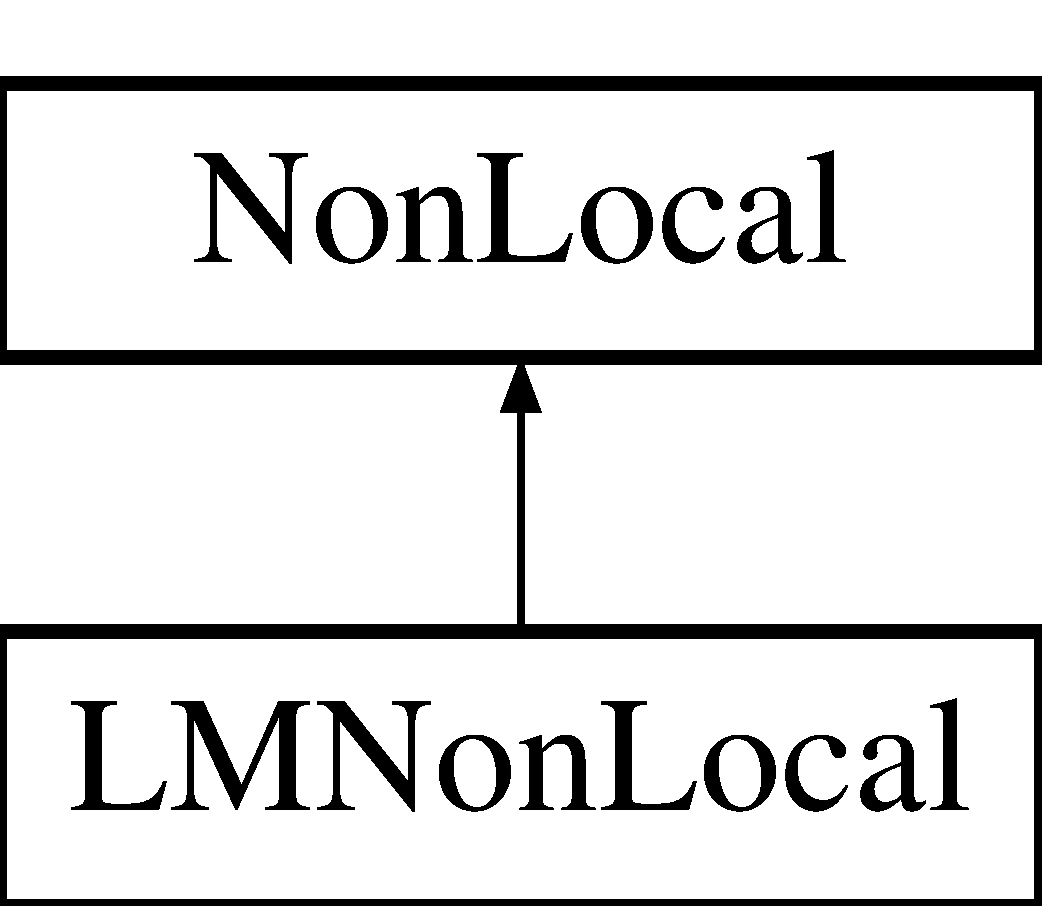
\includegraphics[height=2cm]{classLMNonLocal}
\end{center}
\end{figure}
\subsection*{Public Member Functions}
\begin{DoxyCompactItemize}
\item 
\hypertarget{classLMNonLocal_a7a6000f6118f1c8df727fac29c849b58}{
{\bfseries LMNonLocal} (const \hyperlink{classScarab_1_1HG_1_1HGraph}{HGraph} \&forest, Ngram \&lm, const \hyperlink{classCache}{Cache}$<$ \hyperlink{classScarab_1_1HG_1_1Hypernode}{Hypernode}, int $>$ \&word\_\-cache)}
\label{classLMNonLocal_a7a6000f6118f1c8df727fac29c849b58}

\item 
\hypertarget{classLMNonLocal_a2d14ca694dc6d49ce6e2b80622aafd51}{
void {\bfseries compute} (const \hyperlink{classScarab_1_1HG_1_1Hyperedge}{Hyperedge} \&edge, const vector$<$ vector$<$ int $>$ $>$ \&subder, double \&score, vector$<$ int $>$ \&full\_\-derivation, vector$<$ int $>$ \&sig) const }
\label{classLMNonLocal_a2d14ca694dc6d49ce6e2b80622aafd51}

\item 
\hypertarget{classLMNonLocal_a93334d873bfe91d5357cbec933ec3ae9}{
\hyperlink{structHyp}{Hyp} {\bfseries initialize} (const \hyperlink{classScarab_1_1HG_1_1Hypernode}{Hypernode} \&node) const }
\label{classLMNonLocal_a93334d873bfe91d5357cbec933ec3ae9}

\end{DoxyCompactItemize}


The documentation for this class was generated from the following file:\begin{DoxyCompactItemize}
\item 
CubeLM.h\end{DoxyCompactItemize}

\hypertarget{structLocalHyperedge}{
\section{LocalHyperedge Struct Reference}
\label{structLocalHyperedge}\index{LocalHyperedge@{LocalHyperedge}}
}
\subsection*{Public Attributes}
\begin{DoxyCompactItemize}
\item 
\hypertarget{structLocalHyperedge_a94cbc62434996702ca1d0e28b6dde622}{
vector$<$ int $>$ {\bfseries tail\_\-node\_\-ids}}
\label{structLocalHyperedge_a94cbc62434996702ca1d0e28b6dde622}

\item 
\hypertarget{structLocalHyperedge_a71c8831cc00fefbfb29575856a22fc8a}{
int {\bfseries head}}
\label{structLocalHyperedge_a71c8831cc00fefbfb29575856a22fc8a}

\item 
\hypertarget{structLocalHyperedge_a875e26d7749b13e387b7f0978a4f97a5}{
double {\bfseries weight}}
\label{structLocalHyperedge_a875e26d7749b13e387b7f0978a4f97a5}

\item 
\hypertarget{structLocalHyperedge_ae1b43e113b237128ed95691034ec715e}{
string {\bfseries label}}
\label{structLocalHyperedge_ae1b43e113b237128ed95691034ec715e}

\end{DoxyCompactItemize}


The documentation for this struct was generated from the following file:\begin{DoxyCompactItemize}
\item 
parse/EisnerToHypergraph.h\end{DoxyCompactItemize}

\hypertarget{classLocalTestSuite}{
\section{LocalTestSuite Class Reference}
\label{classLocalTestSuite}\index{LocalTestSuite@{LocalTestSuite}}
}


The documentation for this class was generated from the following file:\begin{DoxyCompactItemize}
\item 
lattice/Test.cpp\end{DoxyCompactItemize}

\hypertarget{structScarab_1_1HG_1_1Location}{
\section{Scarab::HG::Location Struct Reference}
\label{structScarab_1_1HG_1_1Location}\index{Scarab::HG::Location@{Scarab::HG::Location}}
}
\subsection*{Public Member Functions}
\begin{DoxyCompactItemize}
\item 
\hypertarget{structScarab_1_1HG_1_1Location_a66e686eed3a0038886fd24171ec0ae8e}{
void {\bfseries show} ()}
\label{structScarab_1_1HG_1_1Location_a66e686eed3a0038886fd24171ec0ae8e}

\end{DoxyCompactItemize}
\subsection*{Public Attributes}
\begin{DoxyCompactItemize}
\item 
\hypertarget{structScarab_1_1HG_1_1Location_a493249f5c4c2ad6870d1cf1f9dd3f5f5}{
loc {\bfseries location}}
\label{structScarab_1_1HG_1_1Location_a493249f5c4c2ad6870d1cf1f9dd3f5f5}

\item 
\hypertarget{structScarab_1_1HG_1_1Location_a9a11d2d02ffd88048526a28c7619a3c7}{
int {\bfseries node\_\-id}}
\label{structScarab_1_1HG_1_1Location_a9a11d2d02ffd88048526a28c7619a3c7}

\item 
\hypertarget{structScarab_1_1HG_1_1Location_a618dd1682636ccc635ced4dc536be305}{
int {\bfseries edge\_\-id}}
\label{structScarab_1_1HG_1_1Location_a618dd1682636ccc635ced4dc536be305}

\item 
\hypertarget{structScarab_1_1HG_1_1Location_a9e3f8708a3b6c0271a7a854bc6dbde79}{
int {\bfseries edge\_\-pos}}
\label{structScarab_1_1HG_1_1Location_a9e3f8708a3b6c0271a7a854bc6dbde79}

\end{DoxyCompactItemize}


The documentation for this struct was generated from the following file:\begin{DoxyCompactItemize}
\item 
hypergraph/AStar.h\end{DoxyCompactItemize}

\hypertarget{classScarab_1_1HG_1_1LPBuilder}{
\section{Scarab::HG::LPBuilder Class Reference}
\label{classScarab_1_1HG_1_1LPBuilder}\index{Scarab::HG::LPBuilder@{Scarab::HG::LPBuilder}}
}
\subsection*{Public Member Functions}
\begin{DoxyCompactItemize}
\item 
\hypertarget{classScarab_1_1HG_1_1LPBuilder_aba798e4d3faf87e8411607f9d974fc7f}{
{\bfseries LPBuilder} (const \hyperlink{classScarab_1_1HG_1_1HGraph}{HGraph} \&forest, const \hyperlink{classForestLattice}{ForestLattice} \&lat)}
\label{classScarab_1_1HG_1_1LPBuilder_aba798e4d3faf87e8411607f9d974fc7f}

\item 
\hypertarget{classScarab_1_1HG_1_1LPBuilder_abfa755f4c94dc432c022be35861a8200}{
void {\bfseries solve\_\-hypergraph} (const \hyperlink{classCache}{Cache}$<$ \hyperlink{classScarab_1_1HG_1_1Hyperedge}{Hyperedge}, double $>$ \&)}
\label{classScarab_1_1HG_1_1LPBuilder_abfa755f4c94dc432c022be35861a8200}

\item 
\hypertarget{classScarab_1_1HG_1_1LPBuilder_a963bdf9c956b4a08d52be06e1cb6a05a}{
void {\bfseries solve\_\-full} (int run\_\-num, const \hyperlink{classCache}{Cache}$<$ \hyperlink{classScarab_1_1HG_1_1Hyperedge}{Hyperedge}, double $>$ \&\_\-weights, Ngram \&lm, const \hyperlink{classCache}{Cache}$<$ \hyperlink{classScarab_1_1Graph_1_1Graphnode}{Graphnode}, int $>$ \&word\_\-cache)}
\label{classScarab_1_1HG_1_1LPBuilder_a963bdf9c956b4a08d52be06e1cb6a05a}

\end{DoxyCompactItemize}


The documentation for this class was generated from the following files:\begin{DoxyCompactItemize}
\item 
lp/LPBuilder.h\item 
lp/LPBuilder.cpp\end{DoxyCompactItemize}

\hypertarget{classMRF}{
\section{MRF Class Reference}
\label{classMRF}\index{MRF@{MRF}}
}
Inheritance diagram for MRF:\begin{figure}[H]
\begin{center}
\leavevmode
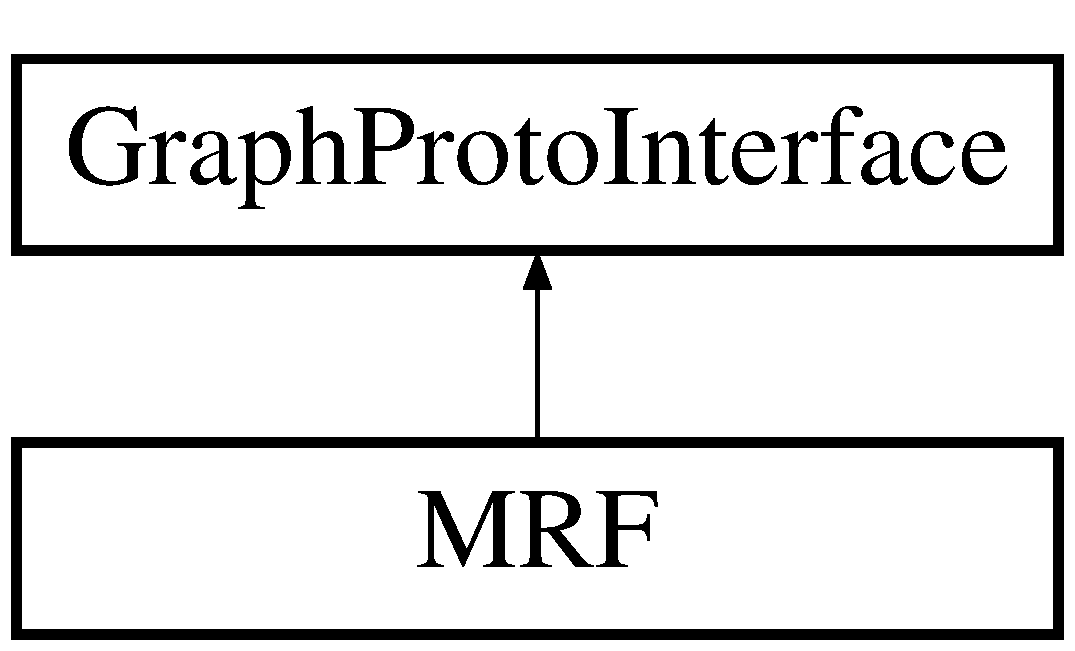
\includegraphics[height=2cm]{classMRF}
\end{center}
\end{figure}
\subsection*{Public Member Functions}
\begin{DoxyCompactItemize}
\item 
\hypertarget{classMRF_a3a2f7eb349a7345abfba2c5869f85b1f}{
void {\bfseries process\_\-node} (graph::Graph\_\-Node, \hyperlink{classScarab_1_1Graph_1_1Graphnode}{Graphnode} $\ast$)}
\label{classMRF_a3a2f7eb349a7345abfba2c5869f85b1f}

\item 
\hypertarget{classMRF_aed7b8a7a2e3af7c14b501040630e9589}{
void {\bfseries process\_\-edge} (graph::Graph\_\-Edge, \hyperlink{classScarab_1_1Graph_1_1Graphedge}{Graphedge} $\ast$)}
\label{classMRF_aed7b8a7a2e3af7c14b501040630e9589}

\item 
\hypertarget{classMRF_a34f0d586337501d668a62726eb0046d7}{
Hypergraph $\ast$ {\bfseries build\_\-hypergraph} ()}
\label{classMRF_a34f0d586337501d668a62726eb0046d7}

\item 
void \hyperlink{classMRF_a928f19f948fa97796462fd9542a985fd}{set\_\-up} (graph::Graph graph, int nodes, int edges)
\item 
\hypertarget{classMRF_a3a7f11091d96ab8b2f830deb343fc3a6}{
const double {\bfseries node\_\-pot} (const \hyperlink{classScarab_1_1Graph_1_1Graphnode}{Graphnode} \&node, const \hyperlink{structState}{State} \&s1) const }
\label{classMRF_a3a7f11091d96ab8b2f830deb343fc3a6}

\item 
\hypertarget{classMRF_ab73d5f7b51c206754bee9eea9405c0fb}{
const bool {\bfseries has\_\-edge\_\-pot} (const \hyperlink{classScarab_1_1Graph_1_1Graphedge}{Graphedge} \&edge, const \hyperlink{structState}{State} \&s1, const \hyperlink{structState}{State} \&s2) const }
\label{classMRF_ab73d5f7b51c206754bee9eea9405c0fb}

\item 
\hypertarget{classMRF_a9f98956295352e9bfc9917328999c1b2}{
const double {\bfseries edge\_\-pot} (const \hyperlink{classScarab_1_1Graph_1_1Graphedge}{Graphedge} \&edge, const \hyperlink{structState}{State} \&s1, const \hyperlink{structState}{State} \&s2) const }
\label{classMRF_a9f98956295352e9bfc9917328999c1b2}

\item 
\hypertarget{classMRF_a7c01a68384b81d1ba7d24508f767d216}{
const vector$<$ \hyperlink{structState}{State} $>$ \& {\bfseries states} (const \hyperlink{classScarab_1_1Graph_1_1Graphnode}{Graphnode} \&node) const }
\label{classMRF_a7c01a68384b81d1ba7d24508f767d216}

\item 
\hypertarget{classMRF_aaf17c4a671ea4f06553c33fca90bfa35}{
const int {\bfseries assignments} () const }
\label{classMRF_aaf17c4a671ea4f06553c33fca90bfa35}

\item 
\hypertarget{classMRF_a9326b3fd5aea915a1bb8a1ad2ac50f3f}{
\hyperlink{structNodeAssignment}{NodeAssignment} {\bfseries make\_\-assignment} (const \hyperlink{classScarab_1_1Graph_1_1Graphnode}{Graphnode} \&n, const \hyperlink{structState}{State} \&my\_\-s) const }
\label{classMRF_a9326b3fd5aea915a1bb8a1ad2ac50f3f}

\end{DoxyCompactItemize}


\subsection{Member Function Documentation}
\hypertarget{classMRF_a928f19f948fa97796462fd9542a985fd}{
\index{MRF@{MRF}!set\_\-up@{set\_\-up}}
\index{set\_\-up@{set\_\-up}!MRF@{MRF}}
\subsubsection[{set\_\-up}]{\setlength{\rightskip}{0pt plus 5cm}void MRF::set\_\-up (graph::Graph {\em graph}, \/  int {\em nodes}, \/  int {\em edges})\hspace{0.3cm}{\ttfamily  \mbox{[}virtual\mbox{]}}}}
\label{classMRF_a928f19f948fa97796462fd9542a985fd}
Solve the potts model with the given node potentials


\begin{DoxyParams}{Parameters}
\item[{\em node\_\-potentials}]\end{DoxyParams}


Reimplemented from \hyperlink{classGraphProtoInterface}{GraphProtoInterface}.



The documentation for this class was generated from the following files:\begin{DoxyCompactItemize}
\item 
optimization/MRF.h\item 
optimization/MRF.cpp\end{DoxyCompactItemize}

\hypertarget{classMRFBuilderLP}{
\section{MRFBuilderLP Class Reference}
\label{classMRFBuilderLP}\index{MRFBuilderLP@{MRFBuilderLP}}
}
\subsection*{Static Public Member Functions}
\begin{DoxyCompactItemize}
\item 
\hypertarget{classMRFBuilderLP_aaace30ed1c0dfb1b0c5c89a22b503e10}{
static \hyperlink{structMRFLP}{MRFLP} $\ast$ {\bfseries add\_\-mrf} (const \hyperlink{classMRF}{MRF} \&mrf, string prefix, GRBModel \&model, int var\_\-type)}
\label{classMRFBuilderLP_aaace30ed1c0dfb1b0c5c89a22b503e10}

\end{DoxyCompactItemize}


The documentation for this class was generated from the following files:\begin{DoxyCompactItemize}
\item 
lp/MRFLP.h\item 
lp/MRFLP.cpp\end{DoxyCompactItemize}

\hypertarget{classgraph_1_1MRFEdge}{
\section{graph::MRFEdge Class Reference}
\label{classgraph_1_1MRFEdge}\index{graph::MRFEdge@{graph::MRFEdge}}
}
\subsection*{Public Member Functions}
\begin{DoxyCompactItemize}
\item 
\hypertarget{classgraph_1_1MRFEdge_aa09de56220ba0cb66c9fd9228ba4d221}{
{\bfseries MRFEdge} (const \hyperlink{classgraph_1_1MRFEdge}{MRFEdge} \&from)}
\label{classgraph_1_1MRFEdge_aa09de56220ba0cb66c9fd9228ba4d221}

\item 
\hypertarget{classgraph_1_1MRFEdge_a3b97945487b8335d0a845629dd61aa9a}{
\hyperlink{classgraph_1_1MRFEdge}{MRFEdge} \& {\bfseries operator=} (const \hyperlink{classgraph_1_1MRFEdge}{MRFEdge} \&from)}
\label{classgraph_1_1MRFEdge_a3b97945487b8335d0a845629dd61aa9a}

\item 
\hypertarget{classgraph_1_1MRFEdge_a291edbf56dd75cfc07882c224d78f6f2}{
const ::google::protobuf::UnknownFieldSet \& {\bfseries unknown\_\-fields} () const }
\label{classgraph_1_1MRFEdge_a291edbf56dd75cfc07882c224d78f6f2}

\item 
\hypertarget{classgraph_1_1MRFEdge_aaf28e2100240ef4b97bff1970da1bbae}{
inline::google::protobuf::UnknownFieldSet $\ast$ {\bfseries mutable\_\-unknown\_\-fields} ()}
\label{classgraph_1_1MRFEdge_aaf28e2100240ef4b97bff1970da1bbae}

\item 
\hypertarget{classgraph_1_1MRFEdge_afded0d8d16e77ef81e494cbdad220734}{
void {\bfseries Swap} (\hyperlink{classgraph_1_1MRFEdge}{MRFEdge} $\ast$other)}
\label{classgraph_1_1MRFEdge_afded0d8d16e77ef81e494cbdad220734}

\item 
\hypertarget{classgraph_1_1MRFEdge_a21211c0e2ad05324c09d90c86b5ba34e}{
\hyperlink{classgraph_1_1MRFEdge}{MRFEdge} $\ast$ {\bfseries New} () const }
\label{classgraph_1_1MRFEdge_a21211c0e2ad05324c09d90c86b5ba34e}

\item 
\hypertarget{classgraph_1_1MRFEdge_a65ec5aa99bae52421400d4b456955ce6}{
void {\bfseries CopyFrom} (const ::google::protobuf::Message \&from)}
\label{classgraph_1_1MRFEdge_a65ec5aa99bae52421400d4b456955ce6}

\item 
\hypertarget{classgraph_1_1MRFEdge_a83fe505e1c12d298d726853b09e566ad}{
void {\bfseries MergeFrom} (const ::google::protobuf::Message \&from)}
\label{classgraph_1_1MRFEdge_a83fe505e1c12d298d726853b09e566ad}

\item 
\hypertarget{classgraph_1_1MRFEdge_a432538f9cc47eaf753e771a1b6cb9a81}{
void {\bfseries CopyFrom} (const \hyperlink{classgraph_1_1MRFEdge}{MRFEdge} \&from)}
\label{classgraph_1_1MRFEdge_a432538f9cc47eaf753e771a1b6cb9a81}

\item 
\hypertarget{classgraph_1_1MRFEdge_a861a18199b5be517a96cd5b355a3c668}{
void {\bfseries MergeFrom} (const \hyperlink{classgraph_1_1MRFEdge}{MRFEdge} \&from)}
\label{classgraph_1_1MRFEdge_a861a18199b5be517a96cd5b355a3c668}

\item 
\hypertarget{classgraph_1_1MRFEdge_ab9d3b2159e6b42fe5fe5f3c4840a151b}{
void {\bfseries Clear} ()}
\label{classgraph_1_1MRFEdge_ab9d3b2159e6b42fe5fe5f3c4840a151b}

\item 
\hypertarget{classgraph_1_1MRFEdge_a11b542bb15495a1fbee395763ee4e22d}{
bool {\bfseries IsInitialized} () const }
\label{classgraph_1_1MRFEdge_a11b542bb15495a1fbee395763ee4e22d}

\item 
\hypertarget{classgraph_1_1MRFEdge_ae857214ec9afbe8246f3027afb231770}{
int {\bfseries ByteSize} () const }
\label{classgraph_1_1MRFEdge_ae857214ec9afbe8246f3027afb231770}

\item 
\hypertarget{classgraph_1_1MRFEdge_abb481822efd72255228c00617b26a9b8}{
bool {\bfseries MergePartialFromCodedStream} (::google::protobuf::io::CodedInputStream $\ast$input)}
\label{classgraph_1_1MRFEdge_abb481822efd72255228c00617b26a9b8}

\item 
\hypertarget{classgraph_1_1MRFEdge_a8b119214980a5375a373bf7acf38f841}{
void {\bfseries SerializeWithCachedSizes} (::google::protobuf::io::CodedOutputStream $\ast$output) const }
\label{classgraph_1_1MRFEdge_a8b119214980a5375a373bf7acf38f841}

\item 
\hypertarget{classgraph_1_1MRFEdge_a5b9122af9f678bf164beab47ca09c7e5}{
::google::protobuf::uint8 $\ast$ {\bfseries SerializeWithCachedSizesToArray} (::google::protobuf::uint8 $\ast$output) const }
\label{classgraph_1_1MRFEdge_a5b9122af9f678bf164beab47ca09c7e5}

\item 
\hypertarget{classgraph_1_1MRFEdge_a2b59a32ff130f0764e937f043fd03778}{
int {\bfseries GetCachedSize} () const }
\label{classgraph_1_1MRFEdge_a2b59a32ff130f0764e937f043fd03778}

\item 
\hypertarget{classgraph_1_1MRFEdge_a3bc4a11c7f89dbff2a95e6f58b0782d9}{
::google::protobuf::Metadata {\bfseries GetMetadata} () const }
\label{classgraph_1_1MRFEdge_a3bc4a11c7f89dbff2a95e6f58b0782d9}

\item 
\hypertarget{classgraph_1_1MRFEdge_ae838e1baabe8852d5ec775f0284ba8b7}{
int {\bfseries edge\_\-potentials\_\-size} () const }
\label{classgraph_1_1MRFEdge_ae838e1baabe8852d5ec775f0284ba8b7}

\item 
\hypertarget{classgraph_1_1MRFEdge_a53d239c44edb18262f0a3c13fd88fb03}{
void {\bfseries clear\_\-edge\_\-potentials} ()}
\label{classgraph_1_1MRFEdge_a53d239c44edb18262f0a3c13fd88fb03}

\item 
\hypertarget{classgraph_1_1MRFEdge_a8dfe87119ec061fe429f4613dd23b1ad}{
const ::\hyperlink{classgraph_1_1EdgeStatePotential}{graph::EdgeStatePotential} \& {\bfseries edge\_\-potentials} (int index) const }
\label{classgraph_1_1MRFEdge_a8dfe87119ec061fe429f4613dd23b1ad}

\item 
\hypertarget{classgraph_1_1MRFEdge_aeff746d072366c703b082307e958d2f0}{
inline::graph::EdgeStatePotential $\ast$ {\bfseries mutable\_\-edge\_\-potentials} (int index)}
\label{classgraph_1_1MRFEdge_aeff746d072366c703b082307e958d2f0}

\item 
\hypertarget{classgraph_1_1MRFEdge_a41a3d93e349503b5d3e24bdc21044810}{
inline::graph::EdgeStatePotential $\ast$ {\bfseries add\_\-edge\_\-potentials} ()}
\label{classgraph_1_1MRFEdge_a41a3d93e349503b5d3e24bdc21044810}

\item 
\hypertarget{classgraph_1_1MRFEdge_a9429ca0ab408685e9d2a955366f50ed6}{
const ::google::protobuf::RepeatedPtrField$<$ ::\hyperlink{classgraph_1_1EdgeStatePotential}{graph::EdgeStatePotential} $>$ \& {\bfseries edge\_\-potentials} () const }
\label{classgraph_1_1MRFEdge_a9429ca0ab408685e9d2a955366f50ed6}

\item 
\hypertarget{classgraph_1_1MRFEdge_a5f8f28def741a8d3476c36eeab872547}{
inline::google::protobuf::RepeatedPtrField$<$ ::\hyperlink{classgraph_1_1EdgeStatePotential}{graph::EdgeStatePotential} $>$ $\ast$ {\bfseries mutable\_\-edge\_\-potentials} ()}
\label{classgraph_1_1MRFEdge_a5f8f28def741a8d3476c36eeab872547}

\item 
\hypertarget{classgraph_1_1MRFEdge_aa09de56220ba0cb66c9fd9228ba4d221}{
{\bfseries MRFEdge} (const \hyperlink{classgraph_1_1MRFEdge}{MRFEdge} \&from)}
\label{classgraph_1_1MRFEdge_aa09de56220ba0cb66c9fd9228ba4d221}

\item 
\hypertarget{classgraph_1_1MRFEdge_a3b97945487b8335d0a845629dd61aa9a}{
\hyperlink{classgraph_1_1MRFEdge}{MRFEdge} \& {\bfseries operator=} (const \hyperlink{classgraph_1_1MRFEdge}{MRFEdge} \&from)}
\label{classgraph_1_1MRFEdge_a3b97945487b8335d0a845629dd61aa9a}

\item 
\hypertarget{classgraph_1_1MRFEdge_a291edbf56dd75cfc07882c224d78f6f2}{
const ::google::protobuf::UnknownFieldSet \& {\bfseries unknown\_\-fields} () const }
\label{classgraph_1_1MRFEdge_a291edbf56dd75cfc07882c224d78f6f2}

\item 
\hypertarget{classgraph_1_1MRFEdge_aaf28e2100240ef4b97bff1970da1bbae}{
inline::google::protobuf::UnknownFieldSet $\ast$ {\bfseries mutable\_\-unknown\_\-fields} ()}
\label{classgraph_1_1MRFEdge_aaf28e2100240ef4b97bff1970da1bbae}

\item 
\hypertarget{classgraph_1_1MRFEdge_afded0d8d16e77ef81e494cbdad220734}{
void {\bfseries Swap} (\hyperlink{classgraph_1_1MRFEdge}{MRFEdge} $\ast$other)}
\label{classgraph_1_1MRFEdge_afded0d8d16e77ef81e494cbdad220734}

\item 
\hypertarget{classgraph_1_1MRFEdge_a21211c0e2ad05324c09d90c86b5ba34e}{
\hyperlink{classgraph_1_1MRFEdge}{MRFEdge} $\ast$ {\bfseries New} () const }
\label{classgraph_1_1MRFEdge_a21211c0e2ad05324c09d90c86b5ba34e}

\item 
\hypertarget{classgraph_1_1MRFEdge_a65ec5aa99bae52421400d4b456955ce6}{
void {\bfseries CopyFrom} (const ::google::protobuf::Message \&from)}
\label{classgraph_1_1MRFEdge_a65ec5aa99bae52421400d4b456955ce6}

\item 
\hypertarget{classgraph_1_1MRFEdge_a83fe505e1c12d298d726853b09e566ad}{
void {\bfseries MergeFrom} (const ::google::protobuf::Message \&from)}
\label{classgraph_1_1MRFEdge_a83fe505e1c12d298d726853b09e566ad}

\item 
\hypertarget{classgraph_1_1MRFEdge_a432538f9cc47eaf753e771a1b6cb9a81}{
void {\bfseries CopyFrom} (const \hyperlink{classgraph_1_1MRFEdge}{MRFEdge} \&from)}
\label{classgraph_1_1MRFEdge_a432538f9cc47eaf753e771a1b6cb9a81}

\item 
\hypertarget{classgraph_1_1MRFEdge_a861a18199b5be517a96cd5b355a3c668}{
void {\bfseries MergeFrom} (const \hyperlink{classgraph_1_1MRFEdge}{MRFEdge} \&from)}
\label{classgraph_1_1MRFEdge_a861a18199b5be517a96cd5b355a3c668}

\item 
\hypertarget{classgraph_1_1MRFEdge_ab9d3b2159e6b42fe5fe5f3c4840a151b}{
void {\bfseries Clear} ()}
\label{classgraph_1_1MRFEdge_ab9d3b2159e6b42fe5fe5f3c4840a151b}

\item 
\hypertarget{classgraph_1_1MRFEdge_a11b542bb15495a1fbee395763ee4e22d}{
bool {\bfseries IsInitialized} () const }
\label{classgraph_1_1MRFEdge_a11b542bb15495a1fbee395763ee4e22d}

\item 
\hypertarget{classgraph_1_1MRFEdge_ae857214ec9afbe8246f3027afb231770}{
int {\bfseries ByteSize} () const }
\label{classgraph_1_1MRFEdge_ae857214ec9afbe8246f3027afb231770}

\item 
\hypertarget{classgraph_1_1MRFEdge_abb481822efd72255228c00617b26a9b8}{
bool {\bfseries MergePartialFromCodedStream} (::google::protobuf::io::CodedInputStream $\ast$input)}
\label{classgraph_1_1MRFEdge_abb481822efd72255228c00617b26a9b8}

\item 
\hypertarget{classgraph_1_1MRFEdge_a8b119214980a5375a373bf7acf38f841}{
void {\bfseries SerializeWithCachedSizes} (::google::protobuf::io::CodedOutputStream $\ast$output) const }
\label{classgraph_1_1MRFEdge_a8b119214980a5375a373bf7acf38f841}

\item 
\hypertarget{classgraph_1_1MRFEdge_a5b9122af9f678bf164beab47ca09c7e5}{
::google::protobuf::uint8 $\ast$ {\bfseries SerializeWithCachedSizesToArray} (::google::protobuf::uint8 $\ast$output) const }
\label{classgraph_1_1MRFEdge_a5b9122af9f678bf164beab47ca09c7e5}

\item 
\hypertarget{classgraph_1_1MRFEdge_a2b59a32ff130f0764e937f043fd03778}{
int {\bfseries GetCachedSize} () const }
\label{classgraph_1_1MRFEdge_a2b59a32ff130f0764e937f043fd03778}

\item 
\hypertarget{classgraph_1_1MRFEdge_a3bc4a11c7f89dbff2a95e6f58b0782d9}{
::google::protobuf::Metadata {\bfseries GetMetadata} () const }
\label{classgraph_1_1MRFEdge_a3bc4a11c7f89dbff2a95e6f58b0782d9}

\item 
\hypertarget{classgraph_1_1MRFEdge_ae838e1baabe8852d5ec775f0284ba8b7}{
int {\bfseries edge\_\-potentials\_\-size} () const }
\label{classgraph_1_1MRFEdge_ae838e1baabe8852d5ec775f0284ba8b7}

\item 
\hypertarget{classgraph_1_1MRFEdge_a53d239c44edb18262f0a3c13fd88fb03}{
void {\bfseries clear\_\-edge\_\-potentials} ()}
\label{classgraph_1_1MRFEdge_a53d239c44edb18262f0a3c13fd88fb03}

\item 
\hypertarget{classgraph_1_1MRFEdge_a0c7561719b73dd2ef987c7c79382f73a}{
const ::\hyperlink{classgraph_1_1EdgeStatePotential}{graph::EdgeStatePotential} \& {\bfseries edge\_\-potentials} (int index) const }
\label{classgraph_1_1MRFEdge_a0c7561719b73dd2ef987c7c79382f73a}

\item 
\hypertarget{classgraph_1_1MRFEdge_af24041a8077b2492fdcbece14538e005}{
inline::graph::EdgeStatePotential $\ast$ {\bfseries mutable\_\-edge\_\-potentials} (int index)}
\label{classgraph_1_1MRFEdge_af24041a8077b2492fdcbece14538e005}

\item 
\hypertarget{classgraph_1_1MRFEdge_a6ae64a2442efe81d52e83b5938820f54}{
inline::graph::EdgeStatePotential $\ast$ {\bfseries add\_\-edge\_\-potentials} ()}
\label{classgraph_1_1MRFEdge_a6ae64a2442efe81d52e83b5938820f54}

\item 
\hypertarget{classgraph_1_1MRFEdge_a11ed986256d3adfc206080df3720d146}{
const ::google::protobuf::RepeatedPtrField$<$ ::\hyperlink{classgraph_1_1EdgeStatePotential}{graph::EdgeStatePotential} $>$ \& {\bfseries edge\_\-potentials} () const }
\label{classgraph_1_1MRFEdge_a11ed986256d3adfc206080df3720d146}

\item 
\hypertarget{classgraph_1_1MRFEdge_ab4e41bd27f096548e580552dbfdb3e35}{
inline::google::protobuf::RepeatedPtrField$<$ ::\hyperlink{classgraph_1_1EdgeStatePotential}{graph::EdgeStatePotential} $>$ $\ast$ {\bfseries mutable\_\-edge\_\-potentials} ()}
\label{classgraph_1_1MRFEdge_ab4e41bd27f096548e580552dbfdb3e35}

\end{DoxyCompactItemize}
\subsection*{Static Public Member Functions}
\begin{DoxyCompactItemize}
\item 
\hypertarget{classgraph_1_1MRFEdge_a9697b3be21e480abdeb24c964934d4cb}{
static const ::google::protobuf::Descriptor $\ast$ {\bfseries descriptor} ()}
\label{classgraph_1_1MRFEdge_a9697b3be21e480abdeb24c964934d4cb}

\item 
\hypertarget{classgraph_1_1MRFEdge_a7375f6abdee806d403d0f0c11a8c86d0}{
static const \hyperlink{classgraph_1_1MRFEdge}{MRFEdge} \& {\bfseries default\_\-instance} ()}
\label{classgraph_1_1MRFEdge_a7375f6abdee806d403d0f0c11a8c86d0}

\item 
\hypertarget{classgraph_1_1MRFEdge_a9697b3be21e480abdeb24c964934d4cb}{
static const ::google::protobuf::Descriptor $\ast$ {\bfseries descriptor} ()}
\label{classgraph_1_1MRFEdge_a9697b3be21e480abdeb24c964934d4cb}

\item 
\hypertarget{classgraph_1_1MRFEdge_a7375f6abdee806d403d0f0c11a8c86d0}{
static const \hyperlink{classgraph_1_1MRFEdge}{MRFEdge} \& {\bfseries default\_\-instance} ()}
\label{classgraph_1_1MRFEdge_a7375f6abdee806d403d0f0c11a8c86d0}

\end{DoxyCompactItemize}
\subsection*{Static Public Attributes}
\begin{DoxyCompactItemize}
\item 
\hypertarget{classgraph_1_1MRFEdge_a8cbb86df3eb46154971fc4d59b9656f3}{
static const int {\bfseries kEdgePotentialsFieldNumber} = 1}
\label{classgraph_1_1MRFEdge_a8cbb86df3eb46154971fc4d59b9656f3}

\end{DoxyCompactItemize}
\subsection*{Friends}
\begin{DoxyCompactItemize}
\item 
\hypertarget{classgraph_1_1MRFEdge_a7c7daba01236a33140ac99dfb4a21f58}{
void {\bfseries protobuf\_\-AddDesc\_\-mrf\_\-2eproto} ()}
\label{classgraph_1_1MRFEdge_a7c7daba01236a33140ac99dfb4a21f58}

\item 
\hypertarget{classgraph_1_1MRFEdge_aef3db81db7837e30d95a050165bc180f}{
void {\bfseries protobuf\_\-AssignDesc\_\-mrf\_\-2eproto} ()}
\label{classgraph_1_1MRFEdge_aef3db81db7837e30d95a050165bc180f}

\item 
\hypertarget{classgraph_1_1MRFEdge_a84e801a5b8303ac698fb7040b250e3d1}{
void {\bfseries protobuf\_\-ShutdownFile\_\-mrf\_\-2eproto} ()}
\label{classgraph_1_1MRFEdge_a84e801a5b8303ac698fb7040b250e3d1}

\item 
\hypertarget{classgraph_1_1MRFEdge_a7c7daba01236a33140ac99dfb4a21f58}{
void {\bfseries protobuf\_\-AddDesc\_\-mrf\_\-2eproto} ()}
\label{classgraph_1_1MRFEdge_a7c7daba01236a33140ac99dfb4a21f58}

\item 
\hypertarget{classgraph_1_1MRFEdge_aef3db81db7837e30d95a050165bc180f}{
void {\bfseries protobuf\_\-AssignDesc\_\-mrf\_\-2eproto} ()}
\label{classgraph_1_1MRFEdge_aef3db81db7837e30d95a050165bc180f}

\item 
\hypertarget{classgraph_1_1MRFEdge_a84e801a5b8303ac698fb7040b250e3d1}{
void {\bfseries protobuf\_\-ShutdownFile\_\-mrf\_\-2eproto} ()}
\label{classgraph_1_1MRFEdge_a84e801a5b8303ac698fb7040b250e3d1}

\end{DoxyCompactItemize}


The documentation for this class was generated from the following files:\begin{DoxyCompactItemize}
\item 
interfaces/graph/gen-\/cpp/mrf.pb.h\item 
interfaces/graph/gen-\/py/mrf.pb.h\end{DoxyCompactItemize}

\hypertarget{classMRFHypergraph}{
\section{MRFHypergraph Class Reference}
\label{classMRFHypergraph}\index{MRFHypergraph@{MRFHypergraph}}
}
Inheritance diagram for MRFHypergraph:\begin{figure}[H]
\begin{center}
\leavevmode
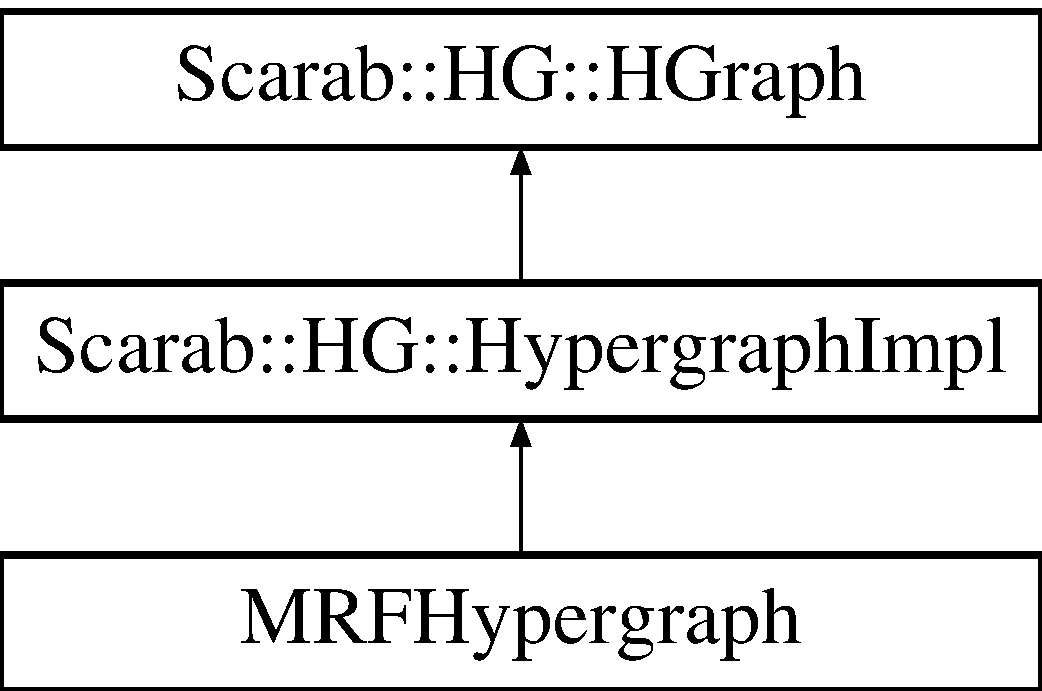
\includegraphics[height=3cm]{classMRFHypergraph}
\end{center}
\end{figure}
\subsection*{Public Member Functions}
\begin{DoxyCompactItemize}
\item 
\hypertarget{classMRFHypergraph_a5c717b35842c25c6be9e827f0aa31708}{
\hyperlink{structNodeAssignment}{NodeAssignment} {\bfseries assignment\_\-from\_\-node} (\hyperlink{classScarab_1_1HG_1_1Hypernode}{Hypernode} $\ast$node)}
\label{classMRFHypergraph_a5c717b35842c25c6be9e827f0aa31708}

\item 
void \hyperlink{classMRFHypergraph_aaac6b68c3ece41ddd1f8107e961879bc}{print} () const 
\item 
\hypertarget{classMRFHypergraph_a34f14a3a9cf0d01c7fbfc11e1caa20ba}{
\hyperlink{classScarab_1_1HG_1_1Hypernode}{HNode} {\bfseries assignment\_\-from\_\-node} (\hyperlink{structNodeAssignment}{NodeAssignment} \&node\_\-assign)}
\label{classMRFHypergraph_a34f14a3a9cf0d01c7fbfc11e1caa20ba}

\end{DoxyCompactItemize}
\subsection*{Static Public Member Functions}
\begin{DoxyCompactItemize}
\item 
\hypertarget{classMRFHypergraph_af8808e644c7ff0c938f4fbd9e473dfba}{
static \hyperlink{classMRFHypergraph}{MRFHypergraph} {\bfseries from\_\-mrf} (const \hyperlink{classMRF}{MRF} \&mrf)}
\label{classMRFHypergraph_af8808e644c7ff0c938f4fbd9e473dfba}

\end{DoxyCompactItemize}


\subsection{Member Function Documentation}
\hypertarget{classMRFHypergraph_aaac6b68c3ece41ddd1f8107e961879bc}{
\index{MRFHypergraph@{MRFHypergraph}!print@{print}}
\index{print@{print}!MRFHypergraph@{MRFHypergraph}}
\subsubsection[{print}]{\setlength{\rightskip}{0pt plus 5cm}void MRFHypergraph::print () const\hspace{0.3cm}{\ttfamily  \mbox{[}inline, virtual\mbox{]}}}}
\label{classMRFHypergraph_aaac6b68c3ece41ddd1f8107e961879bc}
Display the hypergraph for debugging. 

Implements \hyperlink{classScarab_1_1HG_1_1HGraph_ab5aa11c932b28864b56f28e0babbc1c1}{Scarab::HG::HGraph}.



The documentation for this class was generated from the following files:\begin{DoxyCompactItemize}
\item 
optimization/MRFHypergraph.h\item 
optimization/MRFHypergraph.cpp\end{DoxyCompactItemize}

\hypertarget{structMrfIndex}{
\section{MrfIndex Struct Reference}
\label{structMrfIndex}\index{MrfIndex@{MrfIndex}}
}
\subsection*{Public Member Functions}
\begin{DoxyCompactItemize}
\item 
\hypertarget{structMrfIndex_adc62126e39eeccb67aed83b8d33514e9}{
{\bfseries MrfIndex} (int group\_\-, int node\_\-, int state\_\-)}
\label{structMrfIndex_adc62126e39eeccb67aed83b8d33514e9}

\end{DoxyCompactItemize}
\subsection*{Public Attributes}
\begin{DoxyCompactItemize}
\item 
\hypertarget{structMrfIndex_a10be38457b3798cfdf70f224814ce8eb}{
int {\bfseries group}}
\label{structMrfIndex_a10be38457b3798cfdf70f224814ce8eb}

\item 
\hypertarget{structMrfIndex_a9c765fbc8576d8d6541a072eb75c2c8a}{
int {\bfseries node}}
\label{structMrfIndex_a9c765fbc8576d8d6541a072eb75c2c8a}

\item 
\hypertarget{structMrfIndex_a2cea032a5c169945c3c0e8d96fbc1477}{
int {\bfseries state}}
\label{structMrfIndex_a2cea032a5c169945c3c0e8d96fbc1477}

\end{DoxyCompactItemize}


The documentation for this struct was generated from the following file:\begin{DoxyCompactItemize}
\item 
tagger/TagConstraints.h\end{DoxyCompactItemize}

\hypertarget{structMRFLP}{
\section{MRFLP Struct Reference}
\label{structMRFLP}\index{MRFLP@{MRFLP}}
}
\subsection*{Public Member Functions}
\begin{DoxyCompactItemize}
\item 
\hypertarget{structMRFLP_a868a64efdbf8d42682c7953361af4c31}{
{\bfseries MRFLP} (const \hyperlink{classMRF}{MRF} \&p)}
\label{structMRFLP_a868a64efdbf8d42682c7953361af4c31}

\end{DoxyCompactItemize}
\subsection*{Public Attributes}
\begin{DoxyCompactItemize}
\item 
\hypertarget{structMRFLP_a1ddb2cc0eb980dc0d9d94bf731e3f4ae}{
\hyperlink{classCache}{Cache}$<$ \hyperlink{classScarab_1_1Graph_1_1Graphnode}{Graphnode}, \hyperlink{classCache}{Cache}$<$ \hyperlink{structState}{State}, GRBVar $>$ $\ast$ $>$ {\bfseries node\_\-vars}}
\label{structMRFLP_a1ddb2cc0eb980dc0d9d94bf731e3f4ae}

\item 
\hypertarget{structMRFLP_a7f977d31ba7f70b5913279466a46e2b2}{
\hyperlink{classCache}{Cache}$<$ \hyperlink{classScarab_1_1Graph_1_1Graphedge}{Graphedge}, \hyperlink{classCache}{Cache}$<$ \hyperlink{structState}{State}, \hyperlink{classCache}{Cache}$<$ \hyperlink{structState}{State}, GRBVar $>$ $\ast$ $>$ $\ast$ $>$ {\bfseries edge\_\-vars}}
\label{structMRFLP_a7f977d31ba7f70b5913279466a46e2b2}

\item 
\hypertarget{structMRFLP_a46a1042ee20d632ca11afee0a1965fb9}{
\hyperlink{classCache}{Cache}$<$ \hyperlink{classScarab_1_1Graph_1_1Graphedge}{Graphedge}, \hyperlink{classCache}{Cache}$<$ \hyperlink{structState}{State}, GRBVar $>$ $\ast$ $>$ {\bfseries from\_\-state\_\-blank\_\-vars}}
\label{structMRFLP_a46a1042ee20d632ca11afee0a1965fb9}

\item 
\hypertarget{structMRFLP_ae1b4c653d4a3b3c6759a160f8f1c4fc6}{
\hyperlink{classCache}{Cache}$<$ \hyperlink{classScarab_1_1Graph_1_1Graphedge}{Graphedge}, \hyperlink{classCache}{Cache}$<$ \hyperlink{structState}{State}, GRBVar $>$ $\ast$ $>$ {\bfseries to\_\-state\_\-blank\_\-vars}}
\label{structMRFLP_ae1b4c653d4a3b3c6759a160f8f1c4fc6}

\item 
\hypertarget{structMRFLP_a546b7ee8de350e2a882e9ae9beb6af6f}{
const \hyperlink{classMRF}{MRF} \& {\bfseries mrf}}
\label{structMRFLP_a546b7ee8de350e2a882e9ae9beb6af6f}

\end{DoxyCompactItemize}


The documentation for this struct was generated from the following file:\begin{DoxyCompactItemize}
\item 
lp/MRFLP.h\end{DoxyCompactItemize}

\hypertarget{classgraph_1_1MRFNode}{
\section{graph::MRFNode Class Reference}
\label{classgraph_1_1MRFNode}\index{graph::MRFNode@{graph::MRFNode}}
}
\subsection*{Public Member Functions}
\begin{DoxyCompactItemize}
\item 
\hypertarget{classgraph_1_1MRFNode_a021b05b80147363c7e6712f48d44a0a3}{
{\bfseries MRFNode} (const \hyperlink{classgraph_1_1MRFNode}{MRFNode} \&from)}
\label{classgraph_1_1MRFNode_a021b05b80147363c7e6712f48d44a0a3}

\item 
\hypertarget{classgraph_1_1MRFNode_a24e99e7e39879fdb7e5ba3457e05f711}{
\hyperlink{classgraph_1_1MRFNode}{MRFNode} \& {\bfseries operator=} (const \hyperlink{classgraph_1_1MRFNode}{MRFNode} \&from)}
\label{classgraph_1_1MRFNode_a24e99e7e39879fdb7e5ba3457e05f711}

\item 
\hypertarget{classgraph_1_1MRFNode_a8716f067ae2c0b732dbe8e808e58c57f}{
const ::google::protobuf::UnknownFieldSet \& {\bfseries unknown\_\-fields} () const }
\label{classgraph_1_1MRFNode_a8716f067ae2c0b732dbe8e808e58c57f}

\item 
\hypertarget{classgraph_1_1MRFNode_abdd95998aa20cc6e28e69768da470c16}{
inline::google::protobuf::UnknownFieldSet $\ast$ {\bfseries mutable\_\-unknown\_\-fields} ()}
\label{classgraph_1_1MRFNode_abdd95998aa20cc6e28e69768da470c16}

\item 
\hypertarget{classgraph_1_1MRFNode_a6dbf7084428bf6caece3fb82097f1944}{
void {\bfseries Swap} (\hyperlink{classgraph_1_1MRFNode}{MRFNode} $\ast$other)}
\label{classgraph_1_1MRFNode_a6dbf7084428bf6caece3fb82097f1944}

\item 
\hypertarget{classgraph_1_1MRFNode_aae86515fdbc1b37e4e0199213ca28d73}{
\hyperlink{classgraph_1_1MRFNode}{MRFNode} $\ast$ {\bfseries New} () const }
\label{classgraph_1_1MRFNode_aae86515fdbc1b37e4e0199213ca28d73}

\item 
\hypertarget{classgraph_1_1MRFNode_a9597eb49cdf67bc0fcbdf2fd80df98ee}{
void {\bfseries CopyFrom} (const ::google::protobuf::Message \&from)}
\label{classgraph_1_1MRFNode_a9597eb49cdf67bc0fcbdf2fd80df98ee}

\item 
\hypertarget{classgraph_1_1MRFNode_a9c35a74300cf3dca0218bcaeab056068}{
void {\bfseries MergeFrom} (const ::google::protobuf::Message \&from)}
\label{classgraph_1_1MRFNode_a9c35a74300cf3dca0218bcaeab056068}

\item 
\hypertarget{classgraph_1_1MRFNode_ab7f56050e7e981a5aea088fc4703a03b}{
void {\bfseries CopyFrom} (const \hyperlink{classgraph_1_1MRFNode}{MRFNode} \&from)}
\label{classgraph_1_1MRFNode_ab7f56050e7e981a5aea088fc4703a03b}

\item 
\hypertarget{classgraph_1_1MRFNode_ac4758815f0eb1ccb68720627100fbeb5}{
void {\bfseries MergeFrom} (const \hyperlink{classgraph_1_1MRFNode}{MRFNode} \&from)}
\label{classgraph_1_1MRFNode_ac4758815f0eb1ccb68720627100fbeb5}

\item 
\hypertarget{classgraph_1_1MRFNode_a610d843b6af3c9943e096adae1c878b9}{
void {\bfseries Clear} ()}
\label{classgraph_1_1MRFNode_a610d843b6af3c9943e096adae1c878b9}

\item 
\hypertarget{classgraph_1_1MRFNode_a4ee069fb613a4c42ce0b46a092905989}{
bool {\bfseries IsInitialized} () const }
\label{classgraph_1_1MRFNode_a4ee069fb613a4c42ce0b46a092905989}

\item 
\hypertarget{classgraph_1_1MRFNode_ab4cddf5ea1745f095b447d80a7e317b8}{
int {\bfseries ByteSize} () const }
\label{classgraph_1_1MRFNode_ab4cddf5ea1745f095b447d80a7e317b8}

\item 
\hypertarget{classgraph_1_1MRFNode_a7d517e721e300ebe179ef71f53ee2665}{
bool {\bfseries MergePartialFromCodedStream} (::google::protobuf::io::CodedInputStream $\ast$input)}
\label{classgraph_1_1MRFNode_a7d517e721e300ebe179ef71f53ee2665}

\item 
\hypertarget{classgraph_1_1MRFNode_a7d0379969f1c04b3753f3af41fcdcd8d}{
void {\bfseries SerializeWithCachedSizes} (::google::protobuf::io::CodedOutputStream $\ast$output) const }
\label{classgraph_1_1MRFNode_a7d0379969f1c04b3753f3af41fcdcd8d}

\item 
\hypertarget{classgraph_1_1MRFNode_a3c686681d6b3afada8c8119bc167946f}{
::google::protobuf::uint8 $\ast$ {\bfseries SerializeWithCachedSizesToArray} (::google::protobuf::uint8 $\ast$output) const }
\label{classgraph_1_1MRFNode_a3c686681d6b3afada8c8119bc167946f}

\item 
\hypertarget{classgraph_1_1MRFNode_a420b833847841bcbcbbe9baf10d42876}{
int {\bfseries GetCachedSize} () const }
\label{classgraph_1_1MRFNode_a420b833847841bcbcbbe9baf10d42876}

\item 
\hypertarget{classgraph_1_1MRFNode_ad18331d6dffc4a9477fdba263cf9f2fe}{
::google::protobuf::Metadata {\bfseries GetMetadata} () const }
\label{classgraph_1_1MRFNode_ad18331d6dffc4a9477fdba263cf9f2fe}

\item 
\hypertarget{classgraph_1_1MRFNode_aed75e0bf0b6fa5b3ae987510ad1dd75e}{
int {\bfseries node\_\-potentials\_\-size} () const }
\label{classgraph_1_1MRFNode_aed75e0bf0b6fa5b3ae987510ad1dd75e}

\item 
\hypertarget{classgraph_1_1MRFNode_a96a52fa9efd3aa762312bfe27ca05927}{
void {\bfseries clear\_\-node\_\-potentials} ()}
\label{classgraph_1_1MRFNode_a96a52fa9efd3aa762312bfe27ca05927}

\item 
\hypertarget{classgraph_1_1MRFNode_ac1f7d6be6271459b95b37029f8cd31d5}{
const ::\hyperlink{classgraph_1_1NodeStatePotential}{graph::NodeStatePotential} \& {\bfseries node\_\-potentials} (int index) const }
\label{classgraph_1_1MRFNode_ac1f7d6be6271459b95b37029f8cd31d5}

\item 
\hypertarget{classgraph_1_1MRFNode_a9edb6b65ffa1013096b7c47e0efaf0fe}{
inline::graph::NodeStatePotential $\ast$ {\bfseries mutable\_\-node\_\-potentials} (int index)}
\label{classgraph_1_1MRFNode_a9edb6b65ffa1013096b7c47e0efaf0fe}

\item 
\hypertarget{classgraph_1_1MRFNode_ae1315322d7c8e26b8a38cc7ba1bb8d0e}{
inline::graph::NodeStatePotential $\ast$ {\bfseries add\_\-node\_\-potentials} ()}
\label{classgraph_1_1MRFNode_ae1315322d7c8e26b8a38cc7ba1bb8d0e}

\item 
\hypertarget{classgraph_1_1MRFNode_abbecf76da2911c8aa312b7096175c216}{
const ::google::protobuf::RepeatedPtrField$<$ ::\hyperlink{classgraph_1_1NodeStatePotential}{graph::NodeStatePotential} $>$ \& {\bfseries node\_\-potentials} () const }
\label{classgraph_1_1MRFNode_abbecf76da2911c8aa312b7096175c216}

\item 
\hypertarget{classgraph_1_1MRFNode_acb144411ba170fa36398fd55c07b99ca}{
inline::google::protobuf::RepeatedPtrField$<$ ::\hyperlink{classgraph_1_1NodeStatePotential}{graph::NodeStatePotential} $>$ $\ast$ {\bfseries mutable\_\-node\_\-potentials} ()}
\label{classgraph_1_1MRFNode_acb144411ba170fa36398fd55c07b99ca}

\item 
\hypertarget{classgraph_1_1MRFNode_a021b05b80147363c7e6712f48d44a0a3}{
{\bfseries MRFNode} (const \hyperlink{classgraph_1_1MRFNode}{MRFNode} \&from)}
\label{classgraph_1_1MRFNode_a021b05b80147363c7e6712f48d44a0a3}

\item 
\hypertarget{classgraph_1_1MRFNode_a24e99e7e39879fdb7e5ba3457e05f711}{
\hyperlink{classgraph_1_1MRFNode}{MRFNode} \& {\bfseries operator=} (const \hyperlink{classgraph_1_1MRFNode}{MRFNode} \&from)}
\label{classgraph_1_1MRFNode_a24e99e7e39879fdb7e5ba3457e05f711}

\item 
\hypertarget{classgraph_1_1MRFNode_a8716f067ae2c0b732dbe8e808e58c57f}{
const ::google::protobuf::UnknownFieldSet \& {\bfseries unknown\_\-fields} () const }
\label{classgraph_1_1MRFNode_a8716f067ae2c0b732dbe8e808e58c57f}

\item 
\hypertarget{classgraph_1_1MRFNode_abdd95998aa20cc6e28e69768da470c16}{
inline::google::protobuf::UnknownFieldSet $\ast$ {\bfseries mutable\_\-unknown\_\-fields} ()}
\label{classgraph_1_1MRFNode_abdd95998aa20cc6e28e69768da470c16}

\item 
\hypertarget{classgraph_1_1MRFNode_a6dbf7084428bf6caece3fb82097f1944}{
void {\bfseries Swap} (\hyperlink{classgraph_1_1MRFNode}{MRFNode} $\ast$other)}
\label{classgraph_1_1MRFNode_a6dbf7084428bf6caece3fb82097f1944}

\item 
\hypertarget{classgraph_1_1MRFNode_aae86515fdbc1b37e4e0199213ca28d73}{
\hyperlink{classgraph_1_1MRFNode}{MRFNode} $\ast$ {\bfseries New} () const }
\label{classgraph_1_1MRFNode_aae86515fdbc1b37e4e0199213ca28d73}

\item 
\hypertarget{classgraph_1_1MRFNode_a9597eb49cdf67bc0fcbdf2fd80df98ee}{
void {\bfseries CopyFrom} (const ::google::protobuf::Message \&from)}
\label{classgraph_1_1MRFNode_a9597eb49cdf67bc0fcbdf2fd80df98ee}

\item 
\hypertarget{classgraph_1_1MRFNode_a9c35a74300cf3dca0218bcaeab056068}{
void {\bfseries MergeFrom} (const ::google::protobuf::Message \&from)}
\label{classgraph_1_1MRFNode_a9c35a74300cf3dca0218bcaeab056068}

\item 
\hypertarget{classgraph_1_1MRFNode_ab7f56050e7e981a5aea088fc4703a03b}{
void {\bfseries CopyFrom} (const \hyperlink{classgraph_1_1MRFNode}{MRFNode} \&from)}
\label{classgraph_1_1MRFNode_ab7f56050e7e981a5aea088fc4703a03b}

\item 
\hypertarget{classgraph_1_1MRFNode_ac4758815f0eb1ccb68720627100fbeb5}{
void {\bfseries MergeFrom} (const \hyperlink{classgraph_1_1MRFNode}{MRFNode} \&from)}
\label{classgraph_1_1MRFNode_ac4758815f0eb1ccb68720627100fbeb5}

\item 
\hypertarget{classgraph_1_1MRFNode_a610d843b6af3c9943e096adae1c878b9}{
void {\bfseries Clear} ()}
\label{classgraph_1_1MRFNode_a610d843b6af3c9943e096adae1c878b9}

\item 
\hypertarget{classgraph_1_1MRFNode_a4ee069fb613a4c42ce0b46a092905989}{
bool {\bfseries IsInitialized} () const }
\label{classgraph_1_1MRFNode_a4ee069fb613a4c42ce0b46a092905989}

\item 
\hypertarget{classgraph_1_1MRFNode_ab4cddf5ea1745f095b447d80a7e317b8}{
int {\bfseries ByteSize} () const }
\label{classgraph_1_1MRFNode_ab4cddf5ea1745f095b447d80a7e317b8}

\item 
\hypertarget{classgraph_1_1MRFNode_a7d517e721e300ebe179ef71f53ee2665}{
bool {\bfseries MergePartialFromCodedStream} (::google::protobuf::io::CodedInputStream $\ast$input)}
\label{classgraph_1_1MRFNode_a7d517e721e300ebe179ef71f53ee2665}

\item 
\hypertarget{classgraph_1_1MRFNode_a7d0379969f1c04b3753f3af41fcdcd8d}{
void {\bfseries SerializeWithCachedSizes} (::google::protobuf::io::CodedOutputStream $\ast$output) const }
\label{classgraph_1_1MRFNode_a7d0379969f1c04b3753f3af41fcdcd8d}

\item 
\hypertarget{classgraph_1_1MRFNode_a3c686681d6b3afada8c8119bc167946f}{
::google::protobuf::uint8 $\ast$ {\bfseries SerializeWithCachedSizesToArray} (::google::protobuf::uint8 $\ast$output) const }
\label{classgraph_1_1MRFNode_a3c686681d6b3afada8c8119bc167946f}

\item 
\hypertarget{classgraph_1_1MRFNode_a420b833847841bcbcbbe9baf10d42876}{
int {\bfseries GetCachedSize} () const }
\label{classgraph_1_1MRFNode_a420b833847841bcbcbbe9baf10d42876}

\item 
\hypertarget{classgraph_1_1MRFNode_ad18331d6dffc4a9477fdba263cf9f2fe}{
::google::protobuf::Metadata {\bfseries GetMetadata} () const }
\label{classgraph_1_1MRFNode_ad18331d6dffc4a9477fdba263cf9f2fe}

\item 
\hypertarget{classgraph_1_1MRFNode_aed75e0bf0b6fa5b3ae987510ad1dd75e}{
int {\bfseries node\_\-potentials\_\-size} () const }
\label{classgraph_1_1MRFNode_aed75e0bf0b6fa5b3ae987510ad1dd75e}

\item 
\hypertarget{classgraph_1_1MRFNode_a96a52fa9efd3aa762312bfe27ca05927}{
void {\bfseries clear\_\-node\_\-potentials} ()}
\label{classgraph_1_1MRFNode_a96a52fa9efd3aa762312bfe27ca05927}

\item 
\hypertarget{classgraph_1_1MRFNode_a0d51d9a14d08b0044d5bfa9c3d2464b4}{
const ::\hyperlink{classgraph_1_1NodeStatePotential}{graph::NodeStatePotential} \& {\bfseries node\_\-potentials} (int index) const }
\label{classgraph_1_1MRFNode_a0d51d9a14d08b0044d5bfa9c3d2464b4}

\item 
\hypertarget{classgraph_1_1MRFNode_a2592e6dc49b23b2c0cc790cf42921502}{
inline::graph::NodeStatePotential $\ast$ {\bfseries mutable\_\-node\_\-potentials} (int index)}
\label{classgraph_1_1MRFNode_a2592e6dc49b23b2c0cc790cf42921502}

\item 
\hypertarget{classgraph_1_1MRFNode_a942b7f41cd43c7a85fc8bfc6a3bb9714}{
inline::graph::NodeStatePotential $\ast$ {\bfseries add\_\-node\_\-potentials} ()}
\label{classgraph_1_1MRFNode_a942b7f41cd43c7a85fc8bfc6a3bb9714}

\item 
\hypertarget{classgraph_1_1MRFNode_af5c8f3c616fe0bb78485adb1e5482a52}{
const ::google::protobuf::RepeatedPtrField$<$ ::\hyperlink{classgraph_1_1NodeStatePotential}{graph::NodeStatePotential} $>$ \& {\bfseries node\_\-potentials} () const }
\label{classgraph_1_1MRFNode_af5c8f3c616fe0bb78485adb1e5482a52}

\item 
\hypertarget{classgraph_1_1MRFNode_af9736f5670f2b2f12a56501f1dd47446}{
inline::google::protobuf::RepeatedPtrField$<$ ::\hyperlink{classgraph_1_1NodeStatePotential}{graph::NodeStatePotential} $>$ $\ast$ {\bfseries mutable\_\-node\_\-potentials} ()}
\label{classgraph_1_1MRFNode_af9736f5670f2b2f12a56501f1dd47446}

\end{DoxyCompactItemize}
\subsection*{Static Public Member Functions}
\begin{DoxyCompactItemize}
\item 
\hypertarget{classgraph_1_1MRFNode_af65ea7eb633a923f3edb6731d87bc3e0}{
static const ::google::protobuf::Descriptor $\ast$ {\bfseries descriptor} ()}
\label{classgraph_1_1MRFNode_af65ea7eb633a923f3edb6731d87bc3e0}

\item 
\hypertarget{classgraph_1_1MRFNode_ae314d61e7dc907091eb1d67d665888b7}{
static const \hyperlink{classgraph_1_1MRFNode}{MRFNode} \& {\bfseries default\_\-instance} ()}
\label{classgraph_1_1MRFNode_ae314d61e7dc907091eb1d67d665888b7}

\item 
\hypertarget{classgraph_1_1MRFNode_af65ea7eb633a923f3edb6731d87bc3e0}{
static const ::google::protobuf::Descriptor $\ast$ {\bfseries descriptor} ()}
\label{classgraph_1_1MRFNode_af65ea7eb633a923f3edb6731d87bc3e0}

\item 
\hypertarget{classgraph_1_1MRFNode_ae314d61e7dc907091eb1d67d665888b7}{
static const \hyperlink{classgraph_1_1MRFNode}{MRFNode} \& {\bfseries default\_\-instance} ()}
\label{classgraph_1_1MRFNode_ae314d61e7dc907091eb1d67d665888b7}

\end{DoxyCompactItemize}
\subsection*{Static Public Attributes}
\begin{DoxyCompactItemize}
\item 
\hypertarget{classgraph_1_1MRFNode_a8c72fb8318df08ad3774c388ad62296c}{
static const int {\bfseries kNodePotentialsFieldNumber} = 1}
\label{classgraph_1_1MRFNode_a8c72fb8318df08ad3774c388ad62296c}

\end{DoxyCompactItemize}
\subsection*{Friends}
\begin{DoxyCompactItemize}
\item 
\hypertarget{classgraph_1_1MRFNode_a7c7daba01236a33140ac99dfb4a21f58}{
void {\bfseries protobuf\_\-AddDesc\_\-mrf\_\-2eproto} ()}
\label{classgraph_1_1MRFNode_a7c7daba01236a33140ac99dfb4a21f58}

\item 
\hypertarget{classgraph_1_1MRFNode_aef3db81db7837e30d95a050165bc180f}{
void {\bfseries protobuf\_\-AssignDesc\_\-mrf\_\-2eproto} ()}
\label{classgraph_1_1MRFNode_aef3db81db7837e30d95a050165bc180f}

\item 
\hypertarget{classgraph_1_1MRFNode_a84e801a5b8303ac698fb7040b250e3d1}{
void {\bfseries protobuf\_\-ShutdownFile\_\-mrf\_\-2eproto} ()}
\label{classgraph_1_1MRFNode_a84e801a5b8303ac698fb7040b250e3d1}

\item 
\hypertarget{classgraph_1_1MRFNode_a7c7daba01236a33140ac99dfb4a21f58}{
void {\bfseries protobuf\_\-AddDesc\_\-mrf\_\-2eproto} ()}
\label{classgraph_1_1MRFNode_a7c7daba01236a33140ac99dfb4a21f58}

\item 
\hypertarget{classgraph_1_1MRFNode_aef3db81db7837e30d95a050165bc180f}{
void {\bfseries protobuf\_\-AssignDesc\_\-mrf\_\-2eproto} ()}
\label{classgraph_1_1MRFNode_aef3db81db7837e30d95a050165bc180f}

\item 
\hypertarget{classgraph_1_1MRFNode_a84e801a5b8303ac698fb7040b250e3d1}{
void {\bfseries protobuf\_\-ShutdownFile\_\-mrf\_\-2eproto} ()}
\label{classgraph_1_1MRFNode_a84e801a5b8303ac698fb7040b250e3d1}

\end{DoxyCompactItemize}


The documentation for this class was generated from the following files:\begin{DoxyCompactItemize}
\item 
interfaces/graph/gen-\/cpp/mrf.pb.h\item 
interfaces/graph/gen-\/py/mrf.pb.h\end{DoxyCompactItemize}

\hypertarget{classNgramCache}{
\section{NgramCache Class Reference}
\label{classNgramCache}\index{NgramCache@{NgramCache}}
}
\subsection*{Public Member Functions}
\begin{DoxyCompactItemize}
\item 
\hypertarget{classNgramCache_a1d8b66016081c1e0d15b2199e48c4df9}{
{\bfseries NgramCache} (Vocab \&v, int i)}
\label{classNgramCache_a1d8b66016081c1e0d15b2199e48c4df9}

\item 
\hypertarget{classNgramCache_aaf831fb4e48aa1a8f8d46287adb7c419}{
bool {\bfseries hasNext} (const VocabIndex next)}
\label{classNgramCache_aaf831fb4e48aa1a8f8d46287adb7c419}

\item 
\hypertarget{classNgramCache_a3444ab6a1b5a140edb089efb51b071c1}{
LogP {\bfseries wordProbPrimeCache} (VocabIndex word, const VocabIndex $\ast$context)}
\label{classNgramCache_a3444ab6a1b5a140edb089efb51b071c1}

\item 
\hypertarget{classNgramCache_a7806b0a2832644fcde66aa928a58caa9}{
LogP {\bfseries wordProbFromCache} (VocabIndex word, const VocabIndex $\ast$context)}
\label{classNgramCache_a7806b0a2832644fcde66aa928a58caa9}

\end{DoxyCompactItemize}


The documentation for this class was generated from the following files:\begin{DoxyCompactItemize}
\item 
trans\_\-decode/NGramCache.h\item 
trans\_\-decode/NGramCache.cpp\end{DoxyCompactItemize}

\hypertarget{structNodeAssignment}{
\section{NodeAssignment Struct Reference}
\label{structNodeAssignment}\index{NodeAssignment@{NodeAssignment}}
}
\subsection*{Public Member Functions}
\begin{DoxyCompactItemize}
\item 
\hypertarget{structNodeAssignment_afb4f063136a9da957865d42faa2a3943}{
{\bfseries NodeAssignment} (int node\_\-id\_\-, const \hyperlink{structState}{State} state\_\-, int length\_\-)}
\label{structNodeAssignment_afb4f063136a9da957865d42faa2a3943}

\item 
\hypertarget{structNodeAssignment_aea41536d91eba4d9c6440065953aa4e0}{
int {\bfseries id} () const }
\label{structNodeAssignment_aea41536d91eba4d9c6440065953aa4e0}

\end{DoxyCompactItemize}
\subsection*{Public Attributes}
\begin{DoxyCompactItemize}
\item 
\hypertarget{structNodeAssignment_a595045041aa245ed3108284223ce766d}{
int {\bfseries node\_\-id}}
\label{structNodeAssignment_a595045041aa245ed3108284223ce766d}

\item 
\hypertarget{structNodeAssignment_affe9bfbc195ba56f34dcdbd4fb10411e}{
\hyperlink{structState}{State} {\bfseries s}}
\label{structNodeAssignment_affe9bfbc195ba56f34dcdbd4fb10411e}

\item 
\hypertarget{structNodeAssignment_ac3b88ac2cbd270733ee835e00279a4ad}{
int {\bfseries length}}
\label{structNodeAssignment_ac3b88ac2cbd270733ee835e00279a4ad}

\end{DoxyCompactItemize}


The documentation for this struct was generated from the following file:\begin{DoxyCompactItemize}
\item 
optimization/MRF.h\end{DoxyCompactItemize}

\hypertarget{classgraph_1_1NodeStatePotential}{
\section{graph::NodeStatePotential Class Reference}
\label{classgraph_1_1NodeStatePotential}\index{graph::NodeStatePotential@{graph::NodeStatePotential}}
}
\subsection*{Public Member Functions}
\begin{DoxyCompactItemize}
\item 
\hypertarget{classgraph_1_1NodeStatePotential_abe93f0f8c63b6b1861903c72d29bf718}{
{\bfseries NodeStatePotential} (const \hyperlink{classgraph_1_1NodeStatePotential}{NodeStatePotential} \&from)}
\label{classgraph_1_1NodeStatePotential_abe93f0f8c63b6b1861903c72d29bf718}

\item 
\hypertarget{classgraph_1_1NodeStatePotential_a004077f286e88ffafc8b40300d44e201}{
\hyperlink{classgraph_1_1NodeStatePotential}{NodeStatePotential} \& {\bfseries operator=} (const \hyperlink{classgraph_1_1NodeStatePotential}{NodeStatePotential} \&from)}
\label{classgraph_1_1NodeStatePotential_a004077f286e88ffafc8b40300d44e201}

\item 
\hypertarget{classgraph_1_1NodeStatePotential_add63ea9eec1f3caff6ee19c4525e5972}{
const ::google::protobuf::UnknownFieldSet \& {\bfseries unknown\_\-fields} () const }
\label{classgraph_1_1NodeStatePotential_add63ea9eec1f3caff6ee19c4525e5972}

\item 
\hypertarget{classgraph_1_1NodeStatePotential_abb591e0b424e774040f8109c92413f0d}{
inline::google::protobuf::UnknownFieldSet $\ast$ {\bfseries mutable\_\-unknown\_\-fields} ()}
\label{classgraph_1_1NodeStatePotential_abb591e0b424e774040f8109c92413f0d}

\item 
\hypertarget{classgraph_1_1NodeStatePotential_a13b774b1f32294830d162db5e80eb3b7}{
void {\bfseries Swap} (\hyperlink{classgraph_1_1NodeStatePotential}{NodeStatePotential} $\ast$other)}
\label{classgraph_1_1NodeStatePotential_a13b774b1f32294830d162db5e80eb3b7}

\item 
\hypertarget{classgraph_1_1NodeStatePotential_af5fd80aeb33df9a2d08e6fe6b2f6b0e5}{
\hyperlink{classgraph_1_1NodeStatePotential}{NodeStatePotential} $\ast$ {\bfseries New} () const }
\label{classgraph_1_1NodeStatePotential_af5fd80aeb33df9a2d08e6fe6b2f6b0e5}

\item 
\hypertarget{classgraph_1_1NodeStatePotential_ad843be9e9b83a35fa176832eb1bd5b85}{
void {\bfseries CopyFrom} (const ::google::protobuf::Message \&from)}
\label{classgraph_1_1NodeStatePotential_ad843be9e9b83a35fa176832eb1bd5b85}

\item 
\hypertarget{classgraph_1_1NodeStatePotential_a866262febdb1454339ec4c5df39a7638}{
void {\bfseries MergeFrom} (const ::google::protobuf::Message \&from)}
\label{classgraph_1_1NodeStatePotential_a866262febdb1454339ec4c5df39a7638}

\item 
\hypertarget{classgraph_1_1NodeStatePotential_ad9279ae8785df8040b597313593a8693}{
void {\bfseries CopyFrom} (const \hyperlink{classgraph_1_1NodeStatePotential}{NodeStatePotential} \&from)}
\label{classgraph_1_1NodeStatePotential_ad9279ae8785df8040b597313593a8693}

\item 
\hypertarget{classgraph_1_1NodeStatePotential_afed738d7eb798cfa66f0cd24ef51c19f}{
void {\bfseries MergeFrom} (const \hyperlink{classgraph_1_1NodeStatePotential}{NodeStatePotential} \&from)}
\label{classgraph_1_1NodeStatePotential_afed738d7eb798cfa66f0cd24ef51c19f}

\item 
\hypertarget{classgraph_1_1NodeStatePotential_a9f8b12b2fcf2faa5339aa1717a5fb285}{
void {\bfseries Clear} ()}
\label{classgraph_1_1NodeStatePotential_a9f8b12b2fcf2faa5339aa1717a5fb285}

\item 
\hypertarget{classgraph_1_1NodeStatePotential_a22b76e57f65c4389c74ffc73e25beff7}{
bool {\bfseries IsInitialized} () const }
\label{classgraph_1_1NodeStatePotential_a22b76e57f65c4389c74ffc73e25beff7}

\item 
\hypertarget{classgraph_1_1NodeStatePotential_a8a183bdcd7b8a4a0de3d52db9c25c4e9}{
int {\bfseries ByteSize} () const }
\label{classgraph_1_1NodeStatePotential_a8a183bdcd7b8a4a0de3d52db9c25c4e9}

\item 
\hypertarget{classgraph_1_1NodeStatePotential_a23e04477a52de0474588352745d87332}{
bool {\bfseries MergePartialFromCodedStream} (::google::protobuf::io::CodedInputStream $\ast$input)}
\label{classgraph_1_1NodeStatePotential_a23e04477a52de0474588352745d87332}

\item 
\hypertarget{classgraph_1_1NodeStatePotential_a31c56a9c6685e3ebfccf1b20d6126818}{
void {\bfseries SerializeWithCachedSizes} (::google::protobuf::io::CodedOutputStream $\ast$output) const }
\label{classgraph_1_1NodeStatePotential_a31c56a9c6685e3ebfccf1b20d6126818}

\item 
\hypertarget{classgraph_1_1NodeStatePotential_a6ec1fd079d7e4ba59d85aadb77b153a5}{
::google::protobuf::uint8 $\ast$ {\bfseries SerializeWithCachedSizesToArray} (::google::protobuf::uint8 $\ast$output) const }
\label{classgraph_1_1NodeStatePotential_a6ec1fd079d7e4ba59d85aadb77b153a5}

\item 
\hypertarget{classgraph_1_1NodeStatePotential_aed31dd680aeefcc638f69aed20feaa89}{
int {\bfseries GetCachedSize} () const }
\label{classgraph_1_1NodeStatePotential_aed31dd680aeefcc638f69aed20feaa89}

\item 
\hypertarget{classgraph_1_1NodeStatePotential_a9d32e1f4f52612fb611c3cca90461266}{
::google::protobuf::Metadata {\bfseries GetMetadata} () const }
\label{classgraph_1_1NodeStatePotential_a9d32e1f4f52612fb611c3cca90461266}

\item 
\hypertarget{classgraph_1_1NodeStatePotential_a360c4a144fbf3d177d98617b5b680917}{
bool {\bfseries has\_\-state} () const }
\label{classgraph_1_1NodeStatePotential_a360c4a144fbf3d177d98617b5b680917}

\item 
\hypertarget{classgraph_1_1NodeStatePotential_aa742b7c0f5560b3ef8d9a611681cf73f}{
void {\bfseries clear\_\-state} ()}
\label{classgraph_1_1NodeStatePotential_aa742b7c0f5560b3ef8d9a611681cf73f}

\item 
\hypertarget{classgraph_1_1NodeStatePotential_ac914f8afa03faa9de6db823c5f21b7cc}{
const ::\hyperlink{classgraph_1_1State}{graph::State} \& {\bfseries state} () const }
\label{classgraph_1_1NodeStatePotential_ac914f8afa03faa9de6db823c5f21b7cc}

\item 
\hypertarget{classgraph_1_1NodeStatePotential_a8f877868f7590b5be5aae6a78279a75f}{
inline::graph::State $\ast$ {\bfseries mutable\_\-state} ()}
\label{classgraph_1_1NodeStatePotential_a8f877868f7590b5be5aae6a78279a75f}

\item 
\hypertarget{classgraph_1_1NodeStatePotential_a81e5e07ae88c654ef848a8ddfbec8148}{
inline::graph::State $\ast$ {\bfseries release\_\-state} ()}
\label{classgraph_1_1NodeStatePotential_a81e5e07ae88c654ef848a8ddfbec8148}

\item 
\hypertarget{classgraph_1_1NodeStatePotential_a2ef72c30a1c13aa21170eef7a43bde34}{
bool {\bfseries has\_\-node\_\-potential} () const }
\label{classgraph_1_1NodeStatePotential_a2ef72c30a1c13aa21170eef7a43bde34}

\item 
\hypertarget{classgraph_1_1NodeStatePotential_aac3b8f48c1b6320a6381a16d8743073e}{
void {\bfseries clear\_\-node\_\-potential} ()}
\label{classgraph_1_1NodeStatePotential_aac3b8f48c1b6320a6381a16d8743073e}

\item 
\hypertarget{classgraph_1_1NodeStatePotential_a69e4cc64ea70c2153167a1c0f738bfbd}{
float {\bfseries node\_\-potential} () const }
\label{classgraph_1_1NodeStatePotential_a69e4cc64ea70c2153167a1c0f738bfbd}

\item 
\hypertarget{classgraph_1_1NodeStatePotential_a68c6f680cb958390f116dcabb4c0a007}{
void {\bfseries set\_\-node\_\-potential} (float value)}
\label{classgraph_1_1NodeStatePotential_a68c6f680cb958390f116dcabb4c0a007}

\item 
\hypertarget{classgraph_1_1NodeStatePotential_abe93f0f8c63b6b1861903c72d29bf718}{
{\bfseries NodeStatePotential} (const \hyperlink{classgraph_1_1NodeStatePotential}{NodeStatePotential} \&from)}
\label{classgraph_1_1NodeStatePotential_abe93f0f8c63b6b1861903c72d29bf718}

\item 
\hypertarget{classgraph_1_1NodeStatePotential_a004077f286e88ffafc8b40300d44e201}{
\hyperlink{classgraph_1_1NodeStatePotential}{NodeStatePotential} \& {\bfseries operator=} (const \hyperlink{classgraph_1_1NodeStatePotential}{NodeStatePotential} \&from)}
\label{classgraph_1_1NodeStatePotential_a004077f286e88ffafc8b40300d44e201}

\item 
\hypertarget{classgraph_1_1NodeStatePotential_add63ea9eec1f3caff6ee19c4525e5972}{
const ::google::protobuf::UnknownFieldSet \& {\bfseries unknown\_\-fields} () const }
\label{classgraph_1_1NodeStatePotential_add63ea9eec1f3caff6ee19c4525e5972}

\item 
\hypertarget{classgraph_1_1NodeStatePotential_abb591e0b424e774040f8109c92413f0d}{
inline::google::protobuf::UnknownFieldSet $\ast$ {\bfseries mutable\_\-unknown\_\-fields} ()}
\label{classgraph_1_1NodeStatePotential_abb591e0b424e774040f8109c92413f0d}

\item 
\hypertarget{classgraph_1_1NodeStatePotential_a13b774b1f32294830d162db5e80eb3b7}{
void {\bfseries Swap} (\hyperlink{classgraph_1_1NodeStatePotential}{NodeStatePotential} $\ast$other)}
\label{classgraph_1_1NodeStatePotential_a13b774b1f32294830d162db5e80eb3b7}

\item 
\hypertarget{classgraph_1_1NodeStatePotential_af5fd80aeb33df9a2d08e6fe6b2f6b0e5}{
\hyperlink{classgraph_1_1NodeStatePotential}{NodeStatePotential} $\ast$ {\bfseries New} () const }
\label{classgraph_1_1NodeStatePotential_af5fd80aeb33df9a2d08e6fe6b2f6b0e5}

\item 
\hypertarget{classgraph_1_1NodeStatePotential_ad843be9e9b83a35fa176832eb1bd5b85}{
void {\bfseries CopyFrom} (const ::google::protobuf::Message \&from)}
\label{classgraph_1_1NodeStatePotential_ad843be9e9b83a35fa176832eb1bd5b85}

\item 
\hypertarget{classgraph_1_1NodeStatePotential_a866262febdb1454339ec4c5df39a7638}{
void {\bfseries MergeFrom} (const ::google::protobuf::Message \&from)}
\label{classgraph_1_1NodeStatePotential_a866262febdb1454339ec4c5df39a7638}

\item 
\hypertarget{classgraph_1_1NodeStatePotential_ad9279ae8785df8040b597313593a8693}{
void {\bfseries CopyFrom} (const \hyperlink{classgraph_1_1NodeStatePotential}{NodeStatePotential} \&from)}
\label{classgraph_1_1NodeStatePotential_ad9279ae8785df8040b597313593a8693}

\item 
\hypertarget{classgraph_1_1NodeStatePotential_afed738d7eb798cfa66f0cd24ef51c19f}{
void {\bfseries MergeFrom} (const \hyperlink{classgraph_1_1NodeStatePotential}{NodeStatePotential} \&from)}
\label{classgraph_1_1NodeStatePotential_afed738d7eb798cfa66f0cd24ef51c19f}

\item 
\hypertarget{classgraph_1_1NodeStatePotential_a9f8b12b2fcf2faa5339aa1717a5fb285}{
void {\bfseries Clear} ()}
\label{classgraph_1_1NodeStatePotential_a9f8b12b2fcf2faa5339aa1717a5fb285}

\item 
\hypertarget{classgraph_1_1NodeStatePotential_a22b76e57f65c4389c74ffc73e25beff7}{
bool {\bfseries IsInitialized} () const }
\label{classgraph_1_1NodeStatePotential_a22b76e57f65c4389c74ffc73e25beff7}

\item 
\hypertarget{classgraph_1_1NodeStatePotential_a8a183bdcd7b8a4a0de3d52db9c25c4e9}{
int {\bfseries ByteSize} () const }
\label{classgraph_1_1NodeStatePotential_a8a183bdcd7b8a4a0de3d52db9c25c4e9}

\item 
\hypertarget{classgraph_1_1NodeStatePotential_a23e04477a52de0474588352745d87332}{
bool {\bfseries MergePartialFromCodedStream} (::google::protobuf::io::CodedInputStream $\ast$input)}
\label{classgraph_1_1NodeStatePotential_a23e04477a52de0474588352745d87332}

\item 
\hypertarget{classgraph_1_1NodeStatePotential_a31c56a9c6685e3ebfccf1b20d6126818}{
void {\bfseries SerializeWithCachedSizes} (::google::protobuf::io::CodedOutputStream $\ast$output) const }
\label{classgraph_1_1NodeStatePotential_a31c56a9c6685e3ebfccf1b20d6126818}

\item 
\hypertarget{classgraph_1_1NodeStatePotential_a6ec1fd079d7e4ba59d85aadb77b153a5}{
::google::protobuf::uint8 $\ast$ {\bfseries SerializeWithCachedSizesToArray} (::google::protobuf::uint8 $\ast$output) const }
\label{classgraph_1_1NodeStatePotential_a6ec1fd079d7e4ba59d85aadb77b153a5}

\item 
\hypertarget{classgraph_1_1NodeStatePotential_aed31dd680aeefcc638f69aed20feaa89}{
int {\bfseries GetCachedSize} () const }
\label{classgraph_1_1NodeStatePotential_aed31dd680aeefcc638f69aed20feaa89}

\item 
\hypertarget{classgraph_1_1NodeStatePotential_a9d32e1f4f52612fb611c3cca90461266}{
::google::protobuf::Metadata {\bfseries GetMetadata} () const }
\label{classgraph_1_1NodeStatePotential_a9d32e1f4f52612fb611c3cca90461266}

\item 
\hypertarget{classgraph_1_1NodeStatePotential_a360c4a144fbf3d177d98617b5b680917}{
bool {\bfseries has\_\-state} () const }
\label{classgraph_1_1NodeStatePotential_a360c4a144fbf3d177d98617b5b680917}

\item 
\hypertarget{classgraph_1_1NodeStatePotential_aa742b7c0f5560b3ef8d9a611681cf73f}{
void {\bfseries clear\_\-state} ()}
\label{classgraph_1_1NodeStatePotential_aa742b7c0f5560b3ef8d9a611681cf73f}

\item 
\hypertarget{classgraph_1_1NodeStatePotential_aa4662ec90fdc85d9d5eef76b8513ba40}{
const ::\hyperlink{classgraph_1_1State}{graph::State} \& {\bfseries state} () const }
\label{classgraph_1_1NodeStatePotential_aa4662ec90fdc85d9d5eef76b8513ba40}

\item 
\hypertarget{classgraph_1_1NodeStatePotential_a70ac4460fc2c550288b8471d9edddd24}{
inline::graph::State $\ast$ {\bfseries mutable\_\-state} ()}
\label{classgraph_1_1NodeStatePotential_a70ac4460fc2c550288b8471d9edddd24}

\item 
\hypertarget{classgraph_1_1NodeStatePotential_aea68f8c3b4d98f01ac816b5b452ef726}{
inline::graph::State $\ast$ {\bfseries release\_\-state} ()}
\label{classgraph_1_1NodeStatePotential_aea68f8c3b4d98f01ac816b5b452ef726}

\item 
\hypertarget{classgraph_1_1NodeStatePotential_a2ef72c30a1c13aa21170eef7a43bde34}{
bool {\bfseries has\_\-node\_\-potential} () const }
\label{classgraph_1_1NodeStatePotential_a2ef72c30a1c13aa21170eef7a43bde34}

\item 
\hypertarget{classgraph_1_1NodeStatePotential_aac3b8f48c1b6320a6381a16d8743073e}{
void {\bfseries clear\_\-node\_\-potential} ()}
\label{classgraph_1_1NodeStatePotential_aac3b8f48c1b6320a6381a16d8743073e}

\item 
\hypertarget{classgraph_1_1NodeStatePotential_a69e4cc64ea70c2153167a1c0f738bfbd}{
float {\bfseries node\_\-potential} () const }
\label{classgraph_1_1NodeStatePotential_a69e4cc64ea70c2153167a1c0f738bfbd}

\item 
\hypertarget{classgraph_1_1NodeStatePotential_a68c6f680cb958390f116dcabb4c0a007}{
void {\bfseries set\_\-node\_\-potential} (float value)}
\label{classgraph_1_1NodeStatePotential_a68c6f680cb958390f116dcabb4c0a007}

\end{DoxyCompactItemize}
\subsection*{Static Public Member Functions}
\begin{DoxyCompactItemize}
\item 
\hypertarget{classgraph_1_1NodeStatePotential_a376b2186e41466cbaa8dfdb45d5458b0}{
static const ::google::protobuf::Descriptor $\ast$ {\bfseries descriptor} ()}
\label{classgraph_1_1NodeStatePotential_a376b2186e41466cbaa8dfdb45d5458b0}

\item 
\hypertarget{classgraph_1_1NodeStatePotential_a7a7d219bf423b094346b3fd9effb8658}{
static const \hyperlink{classgraph_1_1NodeStatePotential}{NodeStatePotential} \& {\bfseries default\_\-instance} ()}
\label{classgraph_1_1NodeStatePotential_a7a7d219bf423b094346b3fd9effb8658}

\item 
\hypertarget{classgraph_1_1NodeStatePotential_a376b2186e41466cbaa8dfdb45d5458b0}{
static const ::google::protobuf::Descriptor $\ast$ {\bfseries descriptor} ()}
\label{classgraph_1_1NodeStatePotential_a376b2186e41466cbaa8dfdb45d5458b0}

\item 
\hypertarget{classgraph_1_1NodeStatePotential_a7a7d219bf423b094346b3fd9effb8658}{
static const \hyperlink{classgraph_1_1NodeStatePotential}{NodeStatePotential} \& {\bfseries default\_\-instance} ()}
\label{classgraph_1_1NodeStatePotential_a7a7d219bf423b094346b3fd9effb8658}

\end{DoxyCompactItemize}
\subsection*{Static Public Attributes}
\begin{DoxyCompactItemize}
\item 
\hypertarget{classgraph_1_1NodeStatePotential_a265420a2f3c1e9f0eeda17b43ea4d21f}{
static const int {\bfseries kStateFieldNumber} = 1}
\label{classgraph_1_1NodeStatePotential_a265420a2f3c1e9f0eeda17b43ea4d21f}

\item 
\hypertarget{classgraph_1_1NodeStatePotential_a3a181bd7c694d93d54519675fee7218f}{
static const int {\bfseries kNodePotentialFieldNumber} = 2}
\label{classgraph_1_1NodeStatePotential_a3a181bd7c694d93d54519675fee7218f}

\end{DoxyCompactItemize}
\subsection*{Friends}
\begin{DoxyCompactItemize}
\item 
\hypertarget{classgraph_1_1NodeStatePotential_a7c7daba01236a33140ac99dfb4a21f58}{
void {\bfseries protobuf\_\-AddDesc\_\-mrf\_\-2eproto} ()}
\label{classgraph_1_1NodeStatePotential_a7c7daba01236a33140ac99dfb4a21f58}

\item 
\hypertarget{classgraph_1_1NodeStatePotential_aef3db81db7837e30d95a050165bc180f}{
void {\bfseries protobuf\_\-AssignDesc\_\-mrf\_\-2eproto} ()}
\label{classgraph_1_1NodeStatePotential_aef3db81db7837e30d95a050165bc180f}

\item 
\hypertarget{classgraph_1_1NodeStatePotential_a84e801a5b8303ac698fb7040b250e3d1}{
void {\bfseries protobuf\_\-ShutdownFile\_\-mrf\_\-2eproto} ()}
\label{classgraph_1_1NodeStatePotential_a84e801a5b8303ac698fb7040b250e3d1}

\item 
\hypertarget{classgraph_1_1NodeStatePotential_a7c7daba01236a33140ac99dfb4a21f58}{
void {\bfseries protobuf\_\-AddDesc\_\-mrf\_\-2eproto} ()}
\label{classgraph_1_1NodeStatePotential_a7c7daba01236a33140ac99dfb4a21f58}

\item 
\hypertarget{classgraph_1_1NodeStatePotential_aef3db81db7837e30d95a050165bc180f}{
void {\bfseries protobuf\_\-AssignDesc\_\-mrf\_\-2eproto} ()}
\label{classgraph_1_1NodeStatePotential_aef3db81db7837e30d95a050165bc180f}

\item 
\hypertarget{classgraph_1_1NodeStatePotential_a84e801a5b8303ac698fb7040b250e3d1}{
void {\bfseries protobuf\_\-ShutdownFile\_\-mrf\_\-2eproto} ()}
\label{classgraph_1_1NodeStatePotential_a84e801a5b8303ac698fb7040b250e3d1}

\end{DoxyCompactItemize}


The documentation for this class was generated from the following files:\begin{DoxyCompactItemize}
\item 
interfaces/graph/gen-\/cpp/mrf.pb.h\item 
interfaces/graph/gen-\/py/mrf.pb.h\end{DoxyCompactItemize}

\hypertarget{classNonLocal}{
\section{NonLocal Class Reference}
\label{classNonLocal}\index{NonLocal@{NonLocal}}
}
Inheritance diagram for NonLocal:\begin{figure}[H]
\begin{center}
\leavevmode
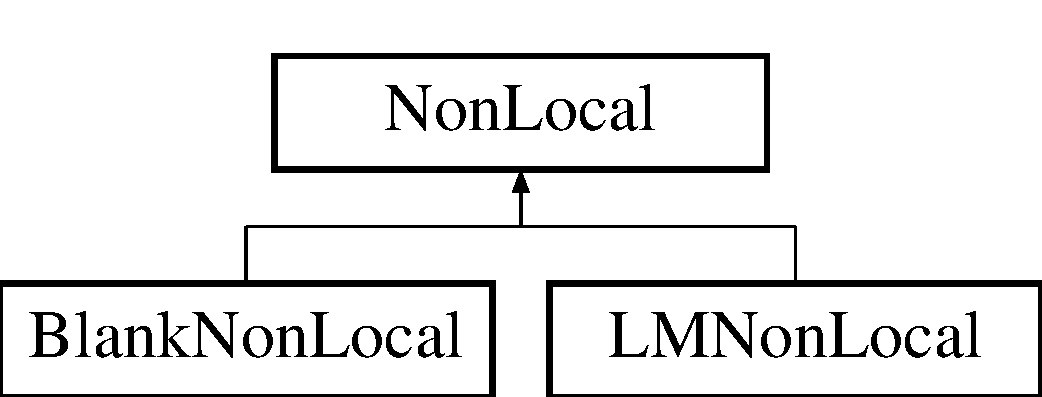
\includegraphics[height=2cm]{classNonLocal}
\end{center}
\end{figure}
\subsection*{Public Member Functions}
\begin{DoxyCompactItemize}
\item 
\hypertarget{classNonLocal_acd66e7882a5bb3415d3fd658d03ec8fc}{
virtual void {\bfseries compute} (const \hyperlink{classScarab_1_1HG_1_1Hyperedge}{Hyperedge} \&, const vector$<$ vector$<$ int $>$ $>$ \&, double \&score, vector$<$ int $>$ \&full\_\-derivation, Sig \&sig) const =0}
\label{classNonLocal_acd66e7882a5bb3415d3fd658d03ec8fc}

\item 
\hypertarget{classNonLocal_a90f2d399853f5c689a0abdc5c12a8370}{
virtual \hyperlink{structHyp}{Hyp} {\bfseries initialize} (const \hyperlink{classScarab_1_1HG_1_1Hypernode}{Hypernode} \&) const =0}
\label{classNonLocal_a90f2d399853f5c689a0abdc5c12a8370}

\end{DoxyCompactItemize}


The documentation for this class was generated from the following file:\begin{DoxyCompactItemize}
\item 
hypergraph/CubePruning.h\end{DoxyCompactItemize}

\hypertarget{classlattice_1_1Origin}{
\section{lattice::Origin Class Reference}
\label{classlattice_1_1Origin}\index{lattice::Origin@{lattice::Origin}}
}
\subsection*{Public Member Functions}
\begin{DoxyCompactItemize}
\item 
\hypertarget{classlattice_1_1Origin_ab55cc18582c3bbc262a924e48697f4cc}{
{\bfseries Origin} (const \hyperlink{classlattice_1_1Origin}{Origin} \&from)}
\label{classlattice_1_1Origin_ab55cc18582c3bbc262a924e48697f4cc}

\item 
\hypertarget{classlattice_1_1Origin_aedeaa82dc76b7d0373cd48f33e028b9e}{
\hyperlink{classlattice_1_1Origin}{Origin} \& {\bfseries operator=} (const \hyperlink{classlattice_1_1Origin}{Origin} \&from)}
\label{classlattice_1_1Origin_aedeaa82dc76b7d0373cd48f33e028b9e}

\item 
\hypertarget{classlattice_1_1Origin_ad520c41793348738a3ac1ebb8f5f1189}{
const ::google::protobuf::UnknownFieldSet \& {\bfseries unknown\_\-fields} () const }
\label{classlattice_1_1Origin_ad520c41793348738a3ac1ebb8f5f1189}

\item 
\hypertarget{classlattice_1_1Origin_a07bec9e32b1ab5ffec8a0fb89f3b593a}{
inline::google::protobuf::UnknownFieldSet $\ast$ {\bfseries mutable\_\-unknown\_\-fields} ()}
\label{classlattice_1_1Origin_a07bec9e32b1ab5ffec8a0fb89f3b593a}

\item 
\hypertarget{classlattice_1_1Origin_a0e3a9e1bbd49641331b067a6dd9e2a8e}{
void {\bfseries Swap} (\hyperlink{classlattice_1_1Origin}{Origin} $\ast$other)}
\label{classlattice_1_1Origin_a0e3a9e1bbd49641331b067a6dd9e2a8e}

\item 
\hypertarget{classlattice_1_1Origin_a8505530533fb46fc7ef7ab26eeb415e6}{
\hyperlink{classlattice_1_1Origin}{Origin} $\ast$ {\bfseries New} () const }
\label{classlattice_1_1Origin_a8505530533fb46fc7ef7ab26eeb415e6}

\item 
\hypertarget{classlattice_1_1Origin_aee8b1f2dd984576e6c73a93d608eb213}{
void {\bfseries CopyFrom} (const ::google::protobuf::Message \&from)}
\label{classlattice_1_1Origin_aee8b1f2dd984576e6c73a93d608eb213}

\item 
\hypertarget{classlattice_1_1Origin_a5b3e6ff8bfb6a4c8e0239774783066b6}{
void {\bfseries MergeFrom} (const ::google::protobuf::Message \&from)}
\label{classlattice_1_1Origin_a5b3e6ff8bfb6a4c8e0239774783066b6}

\item 
\hypertarget{classlattice_1_1Origin_aa91d3c50ddb13b51379510603a068958}{
void {\bfseries CopyFrom} (const \hyperlink{classlattice_1_1Origin}{Origin} \&from)}
\label{classlattice_1_1Origin_aa91d3c50ddb13b51379510603a068958}

\item 
\hypertarget{classlattice_1_1Origin_a3faee262511eec654f7a0632a5e560ba}{
void {\bfseries MergeFrom} (const \hyperlink{classlattice_1_1Origin}{Origin} \&from)}
\label{classlattice_1_1Origin_a3faee262511eec654f7a0632a5e560ba}

\item 
\hypertarget{classlattice_1_1Origin_a90a1a2c78ec1f709cbb0b168fd9aa817}{
void {\bfseries Clear} ()}
\label{classlattice_1_1Origin_a90a1a2c78ec1f709cbb0b168fd9aa817}

\item 
\hypertarget{classlattice_1_1Origin_a62f1d2f32a1eaa899ad85610f1db8fe4}{
bool {\bfseries IsInitialized} () const }
\label{classlattice_1_1Origin_a62f1d2f32a1eaa899ad85610f1db8fe4}

\item 
\hypertarget{classlattice_1_1Origin_af83bae786f9add99760ee4935a135443}{
int {\bfseries ByteSize} () const }
\label{classlattice_1_1Origin_af83bae786f9add99760ee4935a135443}

\item 
\hypertarget{classlattice_1_1Origin_aa13a6b6f63ac1ea4c310f04348a8575f}{
bool {\bfseries MergePartialFromCodedStream} (::google::protobuf::io::CodedInputStream $\ast$input)}
\label{classlattice_1_1Origin_aa13a6b6f63ac1ea4c310f04348a8575f}

\item 
\hypertarget{classlattice_1_1Origin_ae2b055eae68d73af19bcda59c6b15ac6}{
void {\bfseries SerializeWithCachedSizes} (::google::protobuf::io::CodedOutputStream $\ast$output) const }
\label{classlattice_1_1Origin_ae2b055eae68d73af19bcda59c6b15ac6}

\item 
\hypertarget{classlattice_1_1Origin_aeb4b9615f229a32c2476e4528fb1fa6f}{
::google::protobuf::uint8 $\ast$ {\bfseries SerializeWithCachedSizesToArray} (::google::protobuf::uint8 $\ast$output) const }
\label{classlattice_1_1Origin_aeb4b9615f229a32c2476e4528fb1fa6f}

\item 
\hypertarget{classlattice_1_1Origin_a1b84d6bcbe33ca6aa15fc0659fe1ce6c}{
int {\bfseries GetCachedSize} () const }
\label{classlattice_1_1Origin_a1b84d6bcbe33ca6aa15fc0659fe1ce6c}

\item 
\hypertarget{classlattice_1_1Origin_a0f268f800e3755611e74c67e0e81fa73}{
::google::protobuf::Metadata {\bfseries GetMetadata} () const }
\label{classlattice_1_1Origin_a0f268f800e3755611e74c67e0e81fa73}

\item 
\hypertarget{classlattice_1_1Origin_a5a7105c401b9faf2975a62ad0f6e5f9c}{
int {\bfseries hypergraph\_\-edge\_\-size} () const }
\label{classlattice_1_1Origin_a5a7105c401b9faf2975a62ad0f6e5f9c}

\item 
\hypertarget{classlattice_1_1Origin_a16018cbe1e1bda37da1faeda9c113654}{
void {\bfseries clear\_\-hypergraph\_\-edge} ()}
\label{classlattice_1_1Origin_a16018cbe1e1bda37da1faeda9c113654}

\item 
\hypertarget{classlattice_1_1Origin_a5a0033d07d792ad0da3388746bc50dd0}{
inline::google::protobuf::int32 {\bfseries hypergraph\_\-edge} (int index) const }
\label{classlattice_1_1Origin_a5a0033d07d792ad0da3388746bc50dd0}

\item 
\hypertarget{classlattice_1_1Origin_a4ae3e1c5181c4224f9569c7ef916aa94}{
void {\bfseries set\_\-hypergraph\_\-edge} (int index,::google::protobuf::int32 value)}
\label{classlattice_1_1Origin_a4ae3e1c5181c4224f9569c7ef916aa94}

\item 
\hypertarget{classlattice_1_1Origin_adb776f18649e3baa7df68d53dc79bbd6}{
void {\bfseries add\_\-hypergraph\_\-edge} (::google::protobuf::int32 value)}
\label{classlattice_1_1Origin_adb776f18649e3baa7df68d53dc79bbd6}

\item 
\hypertarget{classlattice_1_1Origin_a86672ab29cc9b2b85da694917dd38f2a}{
const ::google::protobuf::RepeatedField$<$ ::google::protobuf::int32 $>$ \& {\bfseries hypergraph\_\-edge} () const }
\label{classlattice_1_1Origin_a86672ab29cc9b2b85da694917dd38f2a}

\item 
\hypertarget{classlattice_1_1Origin_ab9fd75828ae2c7b5188beba8e7d511a5}{
inline::google::protobuf::RepeatedField$<$ ::google::protobuf::int32 $>$ $\ast$ {\bfseries mutable\_\-hypergraph\_\-edge} ()}
\label{classlattice_1_1Origin_ab9fd75828ae2c7b5188beba8e7d511a5}

\item 
\hypertarget{classlattice_1_1Origin_a27d775c4dbd86e55dd6b2bac5f53a194}{
bool {\bfseries has\_\-original\_\-id} () const }
\label{classlattice_1_1Origin_a27d775c4dbd86e55dd6b2bac5f53a194}

\item 
\hypertarget{classlattice_1_1Origin_ae14e0ae4e2b32f4948842a8c64925416}{
void {\bfseries clear\_\-original\_\-id} ()}
\label{classlattice_1_1Origin_ae14e0ae4e2b32f4948842a8c64925416}

\item 
\hypertarget{classlattice_1_1Origin_a0a00308cd28bd4e3836c6a0418276aa5}{
inline::google::protobuf::int32 {\bfseries original\_\-id} () const }
\label{classlattice_1_1Origin_a0a00308cd28bd4e3836c6a0418276aa5}

\item 
\hypertarget{classlattice_1_1Origin_a97ff5372885f733870170f9dfbd3032b}{
void {\bfseries set\_\-original\_\-id} (::google::protobuf::int32 value)}
\label{classlattice_1_1Origin_a97ff5372885f733870170f9dfbd3032b}

\item 
\hypertarget{classlattice_1_1Origin_ad04e2fe74f9c22a83fc22548ade3fd7c}{
bool {\bfseries has\_\-has\_\-origin} () const }
\label{classlattice_1_1Origin_ad04e2fe74f9c22a83fc22548ade3fd7c}

\item 
\hypertarget{classlattice_1_1Origin_ae06e598e03504e3f52a69e1649ef0b84}{
void {\bfseries clear\_\-has\_\-origin} ()}
\label{classlattice_1_1Origin_ae06e598e03504e3f52a69e1649ef0b84}

\item 
\hypertarget{classlattice_1_1Origin_a7b9159f866b74e939a6805a1d765a663}{
bool {\bfseries has\_\-origin} () const }
\label{classlattice_1_1Origin_a7b9159f866b74e939a6805a1d765a663}

\item 
\hypertarget{classlattice_1_1Origin_a7162284423c272a182e8ec697321b97a}{
void {\bfseries set\_\-has\_\-origin} (bool value)}
\label{classlattice_1_1Origin_a7162284423c272a182e8ec697321b97a}

\end{DoxyCompactItemize}
\subsection*{Static Public Member Functions}
\begin{DoxyCompactItemize}
\item 
\hypertarget{classlattice_1_1Origin_aef7714cc60835e8c713096a534ad1d03}{
static const ::google::protobuf::Descriptor $\ast$ {\bfseries descriptor} ()}
\label{classlattice_1_1Origin_aef7714cc60835e8c713096a534ad1d03}

\item 
\hypertarget{classlattice_1_1Origin_a0b2ab113218d71f92d6fda3a8b6c51bc}{
static const \hyperlink{classlattice_1_1Origin}{Origin} \& {\bfseries default\_\-instance} ()}
\label{classlattice_1_1Origin_a0b2ab113218d71f92d6fda3a8b6c51bc}

\end{DoxyCompactItemize}
\subsection*{Static Public Attributes}
\begin{DoxyCompactItemize}
\item 
\hypertarget{classlattice_1_1Origin_a740142917cd1a8dc2db9763c768ea4b1}{
static const int {\bfseries kHypergraphEdgeFieldNumber} = 1}
\label{classlattice_1_1Origin_a740142917cd1a8dc2db9763c768ea4b1}

\item 
\hypertarget{classlattice_1_1Origin_abf5fdc243e613de484e2c64b3ccd0f29}{
static const int {\bfseries kOriginalIdFieldNumber} = 2}
\label{classlattice_1_1Origin_abf5fdc243e613de484e2c64b3ccd0f29}

\item 
\hypertarget{classlattice_1_1Origin_acfa669855c716b2399e9b2949fc38986}{
static const int {\bfseries kHasOriginFieldNumber} = 3}
\label{classlattice_1_1Origin_acfa669855c716b2399e9b2949fc38986}

\end{DoxyCompactItemize}
\subsection*{Friends}
\begin{DoxyCompactItemize}
\item 
\hypertarget{classlattice_1_1Origin_a19e63fb37025879e023cad88064187cf}{
void {\bfseries protobuf\_\-AddDesc\_\-lattice\_\-2eproto} ()}
\label{classlattice_1_1Origin_a19e63fb37025879e023cad88064187cf}

\item 
\hypertarget{classlattice_1_1Origin_a3b0386e09a9fefcf1bdce658cfc480b2}{
void {\bfseries protobuf\_\-AssignDesc\_\-lattice\_\-2eproto} ()}
\label{classlattice_1_1Origin_a3b0386e09a9fefcf1bdce658cfc480b2}

\item 
\hypertarget{classlattice_1_1Origin_a3c7b187721d0704ceb19ff889729d35a}{
void {\bfseries protobuf\_\-ShutdownFile\_\-lattice\_\-2eproto} ()}
\label{classlattice_1_1Origin_a3c7b187721d0704ceb19ff889729d35a}

\end{DoxyCompactItemize}


The documentation for this class was generated from the following file:\begin{DoxyCompactItemize}
\item 
interfaces/lattice/gen-\/cpp/lattice.pb.h\end{DoxyCompactItemize}

\hypertarget{classPhraseBased}{
\section{PhraseBased Class Reference}
\label{classPhraseBased}\index{PhraseBased@{PhraseBased}}
}
Inheritance diagram for PhraseBased:\begin{figure}[H]
\begin{center}
\leavevmode
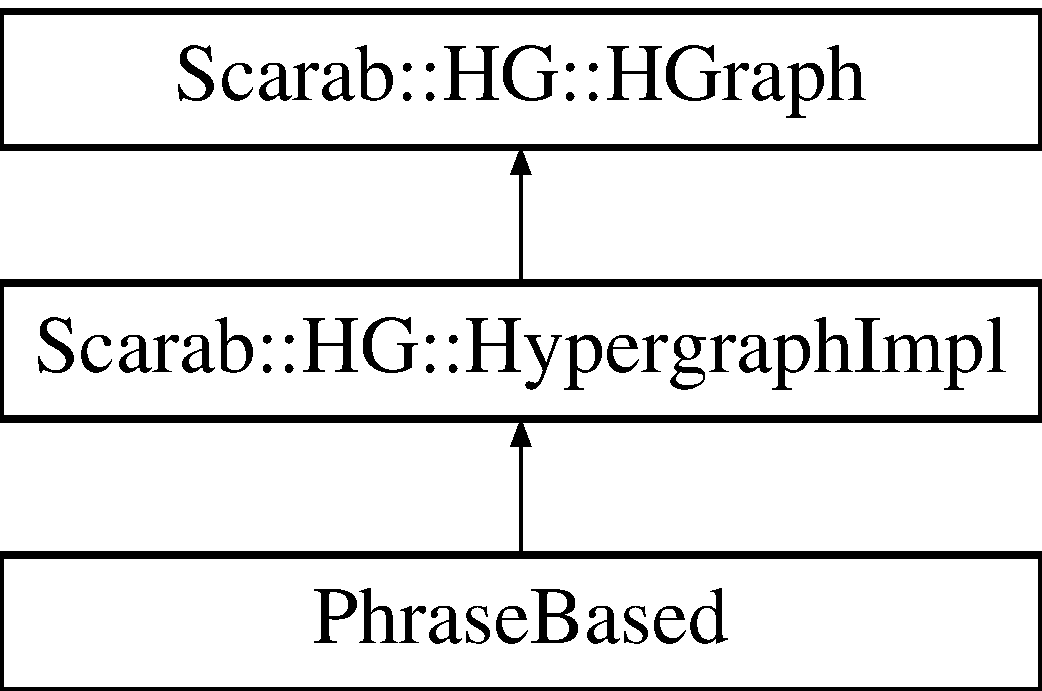
\includegraphics[height=3cm]{classPhraseBased}
\end{center}
\end{figure}
\subsection*{Public Member Functions}
\begin{DoxyCompactItemize}
\item 
void \hyperlink{classPhraseBased_aafc2997b58b3698fed7cb5a1f6f269c6}{print} () const 
\item 
\hypertarget{classPhraseBased_a3883660c72be6ce8daab08f368317853}{
void {\bfseries set\_\-up} (const Hypergraph \&hgraph)}
\label{classPhraseBased_a3883660c72be6ce8daab08f368317853}

\end{DoxyCompactItemize}


\subsection{Member Function Documentation}
\hypertarget{classPhraseBased_aafc2997b58b3698fed7cb5a1f6f269c6}{
\index{PhraseBased@{PhraseBased}!print@{print}}
\index{print@{print}!PhraseBased@{PhraseBased}}
\subsubsection[{print}]{\setlength{\rightskip}{0pt plus 5cm}void PhraseBased::print () const\hspace{0.3cm}{\ttfamily  \mbox{[}inline, virtual\mbox{]}}}}
\label{classPhraseBased_aafc2997b58b3698fed7cb5a1f6f269c6}
Display the hypergraph for debugging. 

Implements \hyperlink{classScarab_1_1HG_1_1HGraph_ab5aa11c932b28864b56f28e0babbc1c1}{Scarab::HG::HGraph}.



The documentation for this class was generated from the following file:\begin{DoxyCompactItemize}
\item 
phrasebased/PhraseBased.h\end{DoxyCompactItemize}

\hypertarget{classlattice_1_1Phraselet}{
\section{lattice::Phraselet Class Reference}
\label{classlattice_1_1Phraselet}\index{lattice::Phraselet@{lattice::Phraselet}}
}
\subsection*{Public Member Functions}
\begin{DoxyCompactItemize}
\item 
\hypertarget{classlattice_1_1Phraselet_aad52fffee57cf2c3c738db3911eb4bb9}{
{\bfseries Phraselet} (const \hyperlink{classlattice_1_1Phraselet}{Phraselet} \&from)}
\label{classlattice_1_1Phraselet_aad52fffee57cf2c3c738db3911eb4bb9}

\item 
\hypertarget{classlattice_1_1Phraselet_a351df01d2ffbf4f31cac03ee8c1fc237}{
\hyperlink{classlattice_1_1Phraselet}{Phraselet} \& {\bfseries operator=} (const \hyperlink{classlattice_1_1Phraselet}{Phraselet} \&from)}
\label{classlattice_1_1Phraselet_a351df01d2ffbf4f31cac03ee8c1fc237}

\item 
\hypertarget{classlattice_1_1Phraselet_ad493e6fbf47ab949e24f807b94232c64}{
const ::google::protobuf::UnknownFieldSet \& {\bfseries unknown\_\-fields} () const }
\label{classlattice_1_1Phraselet_ad493e6fbf47ab949e24f807b94232c64}

\item 
\hypertarget{classlattice_1_1Phraselet_a92f57adf0baa33f5152ee431b1aea6e1}{
inline::google::protobuf::UnknownFieldSet $\ast$ {\bfseries mutable\_\-unknown\_\-fields} ()}
\label{classlattice_1_1Phraselet_a92f57adf0baa33f5152ee431b1aea6e1}

\item 
\hypertarget{classlattice_1_1Phraselet_a475dcd429c962649f7f26e9cbd8d5a34}{
void {\bfseries Swap} (\hyperlink{classlattice_1_1Phraselet}{Phraselet} $\ast$other)}
\label{classlattice_1_1Phraselet_a475dcd429c962649f7f26e9cbd8d5a34}

\item 
\hypertarget{classlattice_1_1Phraselet_a6e0f65c2f64009750641683f3320d739}{
\hyperlink{classlattice_1_1Phraselet}{Phraselet} $\ast$ {\bfseries New} () const }
\label{classlattice_1_1Phraselet_a6e0f65c2f64009750641683f3320d739}

\item 
\hypertarget{classlattice_1_1Phraselet_a2d367abbea6d71d9ffaf3457661b5a42}{
void {\bfseries CopyFrom} (const ::google::protobuf::Message \&from)}
\label{classlattice_1_1Phraselet_a2d367abbea6d71d9ffaf3457661b5a42}

\item 
\hypertarget{classlattice_1_1Phraselet_a381bcf822ebd538c59bf795dee2b77d9}{
void {\bfseries MergeFrom} (const ::google::protobuf::Message \&from)}
\label{classlattice_1_1Phraselet_a381bcf822ebd538c59bf795dee2b77d9}

\item 
\hypertarget{classlattice_1_1Phraselet_aa8bc3ab3f900bfdff4a4134031218fc3}{
void {\bfseries CopyFrom} (const \hyperlink{classlattice_1_1Phraselet}{Phraselet} \&from)}
\label{classlattice_1_1Phraselet_aa8bc3ab3f900bfdff4a4134031218fc3}

\item 
\hypertarget{classlattice_1_1Phraselet_aea4c86bf72b788b9afec402442f963df}{
void {\bfseries MergeFrom} (const \hyperlink{classlattice_1_1Phraselet}{Phraselet} \&from)}
\label{classlattice_1_1Phraselet_aea4c86bf72b788b9afec402442f963df}

\item 
\hypertarget{classlattice_1_1Phraselet_a380c5bf45d45269bc0ec61e80c4df34e}{
void {\bfseries Clear} ()}
\label{classlattice_1_1Phraselet_a380c5bf45d45269bc0ec61e80c4df34e}

\item 
\hypertarget{classlattice_1_1Phraselet_aa25d46e3d15cb431d4a7cf30c8ad5bdb}{
bool {\bfseries IsInitialized} () const }
\label{classlattice_1_1Phraselet_aa25d46e3d15cb431d4a7cf30c8ad5bdb}

\item 
\hypertarget{classlattice_1_1Phraselet_a6b23edd221a64e6553d042f45df86e73}{
int {\bfseries ByteSize} () const }
\label{classlattice_1_1Phraselet_a6b23edd221a64e6553d042f45df86e73}

\item 
\hypertarget{classlattice_1_1Phraselet_af794c511c8d6be67e141a790ce18ef6f}{
bool {\bfseries MergePartialFromCodedStream} (::google::protobuf::io::CodedInputStream $\ast$input)}
\label{classlattice_1_1Phraselet_af794c511c8d6be67e141a790ce18ef6f}

\item 
\hypertarget{classlattice_1_1Phraselet_a00627ab143b2b8d5fcbdc686b2496230}{
void {\bfseries SerializeWithCachedSizes} (::google::protobuf::io::CodedOutputStream $\ast$output) const }
\label{classlattice_1_1Phraselet_a00627ab143b2b8d5fcbdc686b2496230}

\item 
\hypertarget{classlattice_1_1Phraselet_ac1261f6fa5635a6dc867b5afcbbce2c0}{
::google::protobuf::uint8 $\ast$ {\bfseries SerializeWithCachedSizesToArray} (::google::protobuf::uint8 $\ast$output) const }
\label{classlattice_1_1Phraselet_ac1261f6fa5635a6dc867b5afcbbce2c0}

\item 
\hypertarget{classlattice_1_1Phraselet_ae94d4b81c0ae8e195346f0b2836fa124}{
int {\bfseries GetCachedSize} () const }
\label{classlattice_1_1Phraselet_ae94d4b81c0ae8e195346f0b2836fa124}

\item 
\hypertarget{classlattice_1_1Phraselet_a604a20b0d6799e17708325a49dbd89ee}{
::google::protobuf::Metadata {\bfseries GetMetadata} () const }
\label{classlattice_1_1Phraselet_a604a20b0d6799e17708325a49dbd89ee}

\item 
\hypertarget{classlattice_1_1Phraselet_a5136efd90a23878ff47bb0290c5f9678}{
int {\bfseries word\_\-size} () const }
\label{classlattice_1_1Phraselet_a5136efd90a23878ff47bb0290c5f9678}

\item 
\hypertarget{classlattice_1_1Phraselet_a2ac956bf60b94eab43cb142bb2251731}{
void {\bfseries clear\_\-word} ()}
\label{classlattice_1_1Phraselet_a2ac956bf60b94eab43cb142bb2251731}

\item 
\hypertarget{classlattice_1_1Phraselet_a39c2b7f8be4d23aa423baf985107a0be}{
const ::\hyperlink{classlattice_1_1Subword}{lattice::Subword} \& {\bfseries word} (int index) const }
\label{classlattice_1_1Phraselet_a39c2b7f8be4d23aa423baf985107a0be}

\item 
\hypertarget{classlattice_1_1Phraselet_abe2be887d98594a7c3ce13844b8a87f3}{
inline::lattice::Subword $\ast$ {\bfseries mutable\_\-word} (int index)}
\label{classlattice_1_1Phraselet_abe2be887d98594a7c3ce13844b8a87f3}

\item 
\hypertarget{classlattice_1_1Phraselet_af499ae2b30d9739234523c9d790e07eb}{
inline::lattice::Subword $\ast$ {\bfseries add\_\-word} ()}
\label{classlattice_1_1Phraselet_af499ae2b30d9739234523c9d790e07eb}

\item 
\hypertarget{classlattice_1_1Phraselet_ad442b1e821ee49c64e44191d32200e60}{
const ::google::protobuf::RepeatedPtrField$<$ ::\hyperlink{classlattice_1_1Subword}{lattice::Subword} $>$ \& {\bfseries word} () const }
\label{classlattice_1_1Phraselet_ad442b1e821ee49c64e44191d32200e60}

\item 
\hypertarget{classlattice_1_1Phraselet_a4789a16818260e9df5f6cf5b954e70ee}{
inline::google::protobuf::RepeatedPtrField$<$ ::\hyperlink{classlattice_1_1Subword}{lattice::Subword} $>$ $\ast$ {\bfseries mutable\_\-word} ()}
\label{classlattice_1_1Phraselet_a4789a16818260e9df5f6cf5b954e70ee}

\item 
\hypertarget{classlattice_1_1Phraselet_a9a6afc2d0f7466317b7bbd0ebe8eb5d4}{
bool {\bfseries has\_\-phraselet\_\-hypergraph\_\-edge} () const }
\label{classlattice_1_1Phraselet_a9a6afc2d0f7466317b7bbd0ebe8eb5d4}

\item 
\hypertarget{classlattice_1_1Phraselet_a4c9f2577858563c51a8531604e30b1a7}{
void {\bfseries clear\_\-phraselet\_\-hypergraph\_\-edge} ()}
\label{classlattice_1_1Phraselet_a4c9f2577858563c51a8531604e30b1a7}

\item 
\hypertarget{classlattice_1_1Phraselet_a36ecf9680559a4cfdb011c8531830220}{
inline::google::protobuf::int32 {\bfseries phraselet\_\-hypergraph\_\-edge} () const }
\label{classlattice_1_1Phraselet_a36ecf9680559a4cfdb011c8531830220}

\item 
\hypertarget{classlattice_1_1Phraselet_ae9112854c9a8406aeef40c13f9c8b02a}{
void {\bfseries set\_\-phraselet\_\-hypergraph\_\-edge} (::google::protobuf::int32 value)}
\label{classlattice_1_1Phraselet_ae9112854c9a8406aeef40c13f9c8b02a}

\end{DoxyCompactItemize}
\subsection*{Static Public Member Functions}
\begin{DoxyCompactItemize}
\item 
\hypertarget{classlattice_1_1Phraselet_a8b9fdd34efe3ebab08aba8b6b2dfc927}{
static const ::google::protobuf::Descriptor $\ast$ {\bfseries descriptor} ()}
\label{classlattice_1_1Phraselet_a8b9fdd34efe3ebab08aba8b6b2dfc927}

\item 
\hypertarget{classlattice_1_1Phraselet_a64a4092d90a733f714a7d0371b4faa24}{
static const \hyperlink{classlattice_1_1Phraselet}{Phraselet} \& {\bfseries default\_\-instance} ()}
\label{classlattice_1_1Phraselet_a64a4092d90a733f714a7d0371b4faa24}

\end{DoxyCompactItemize}
\subsection*{Static Public Attributes}
\begin{DoxyCompactItemize}
\item 
\hypertarget{classlattice_1_1Phraselet_abc30d76e181d14e5a53cee96bdd50eda}{
static const int {\bfseries kWordFieldNumber} = 1}
\label{classlattice_1_1Phraselet_abc30d76e181d14e5a53cee96bdd50eda}

\item 
\hypertarget{classlattice_1_1Phraselet_a99ae4ed782afdeef679118bef7361c00}{
static const int {\bfseries kPhraseletHypergraphEdgeFieldNumber} = 2}
\label{classlattice_1_1Phraselet_a99ae4ed782afdeef679118bef7361c00}

\end{DoxyCompactItemize}
\subsection*{Friends}
\begin{DoxyCompactItemize}
\item 
\hypertarget{classlattice_1_1Phraselet_a19e63fb37025879e023cad88064187cf}{
void {\bfseries protobuf\_\-AddDesc\_\-lattice\_\-2eproto} ()}
\label{classlattice_1_1Phraselet_a19e63fb37025879e023cad88064187cf}

\item 
\hypertarget{classlattice_1_1Phraselet_a3b0386e09a9fefcf1bdce658cfc480b2}{
void {\bfseries protobuf\_\-AssignDesc\_\-lattice\_\-2eproto} ()}
\label{classlattice_1_1Phraselet_a3b0386e09a9fefcf1bdce658cfc480b2}

\item 
\hypertarget{classlattice_1_1Phraselet_a3c7b187721d0704ceb19ff889729d35a}{
void {\bfseries protobuf\_\-ShutdownFile\_\-lattice\_\-2eproto} ()}
\label{classlattice_1_1Phraselet_a3c7b187721d0704ceb19ff889729d35a}

\end{DoxyCompactItemize}


The documentation for this class was generated from the following file:\begin{DoxyCompactItemize}
\item 
interfaces/lattice/gen-\/cpp/lattice.pb.h\end{DoxyCompactItemize}

\hypertarget{classlattice_1_1Phraselets}{
\section{lattice::Phraselets Class Reference}
\label{classlattice_1_1Phraselets}\index{lattice::Phraselets@{lattice::Phraselets}}
}
\subsection*{Public Member Functions}
\begin{DoxyCompactItemize}
\item 
\hypertarget{classlattice_1_1Phraselets_ab7dd94e765222f9afd3ddc6aae28f4b9}{
{\bfseries Phraselets} (const \hyperlink{classlattice_1_1Phraselets}{Phraselets} \&from)}
\label{classlattice_1_1Phraselets_ab7dd94e765222f9afd3ddc6aae28f4b9}

\item 
\hypertarget{classlattice_1_1Phraselets_ab7fc4048a36fb485457156b33d201f0f}{
\hyperlink{classlattice_1_1Phraselets}{Phraselets} \& {\bfseries operator=} (const \hyperlink{classlattice_1_1Phraselets}{Phraselets} \&from)}
\label{classlattice_1_1Phraselets_ab7fc4048a36fb485457156b33d201f0f}

\item 
\hypertarget{classlattice_1_1Phraselets_a2139960d920a5bc3aa8b93eee034a5f3}{
const ::google::protobuf::UnknownFieldSet \& {\bfseries unknown\_\-fields} () const }
\label{classlattice_1_1Phraselets_a2139960d920a5bc3aa8b93eee034a5f3}

\item 
\hypertarget{classlattice_1_1Phraselets_a30f7480fb64d1b726d53ee8bea076b72}{
inline::google::protobuf::UnknownFieldSet $\ast$ {\bfseries mutable\_\-unknown\_\-fields} ()}
\label{classlattice_1_1Phraselets_a30f7480fb64d1b726d53ee8bea076b72}

\item 
\hypertarget{classlattice_1_1Phraselets_af2b24704a495960845fe4e4c2188a53f}{
void {\bfseries Swap} (\hyperlink{classlattice_1_1Phraselets}{Phraselets} $\ast$other)}
\label{classlattice_1_1Phraselets_af2b24704a495960845fe4e4c2188a53f}

\item 
\hypertarget{classlattice_1_1Phraselets_a8229047c413dbe2af7836e10c8b4c0d4}{
\hyperlink{classlattice_1_1Phraselets}{Phraselets} $\ast$ {\bfseries New} () const }
\label{classlattice_1_1Phraselets_a8229047c413dbe2af7836e10c8b4c0d4}

\item 
\hypertarget{classlattice_1_1Phraselets_ae545b608108f883959885ca212ba9c47}{
void {\bfseries CopyFrom} (const ::google::protobuf::Message \&from)}
\label{classlattice_1_1Phraselets_ae545b608108f883959885ca212ba9c47}

\item 
\hypertarget{classlattice_1_1Phraselets_aea0701d2263901e124d9f4eb0ebb586e}{
void {\bfseries MergeFrom} (const ::google::protobuf::Message \&from)}
\label{classlattice_1_1Phraselets_aea0701d2263901e124d9f4eb0ebb586e}

\item 
\hypertarget{classlattice_1_1Phraselets_ac35d667378bb57992378580af8e2a42b}{
void {\bfseries CopyFrom} (const \hyperlink{classlattice_1_1Phraselets}{Phraselets} \&from)}
\label{classlattice_1_1Phraselets_ac35d667378bb57992378580af8e2a42b}

\item 
\hypertarget{classlattice_1_1Phraselets_a09cc9a5dad7bad0248ab26275d7d3151}{
void {\bfseries MergeFrom} (const \hyperlink{classlattice_1_1Phraselets}{Phraselets} \&from)}
\label{classlattice_1_1Phraselets_a09cc9a5dad7bad0248ab26275d7d3151}

\item 
\hypertarget{classlattice_1_1Phraselets_a4c735228e79edaf401ac7d08d35b53ac}{
void {\bfseries Clear} ()}
\label{classlattice_1_1Phraselets_a4c735228e79edaf401ac7d08d35b53ac}

\item 
\hypertarget{classlattice_1_1Phraselets_a4a9cdf5ab0725a87acb7831f572878ee}{
bool {\bfseries IsInitialized} () const }
\label{classlattice_1_1Phraselets_a4a9cdf5ab0725a87acb7831f572878ee}

\item 
\hypertarget{classlattice_1_1Phraselets_a26f51d307c09dc6a01c1c3a83afa898d}{
int {\bfseries ByteSize} () const }
\label{classlattice_1_1Phraselets_a26f51d307c09dc6a01c1c3a83afa898d}

\item 
\hypertarget{classlattice_1_1Phraselets_aa939d6bdfd0a634d857f62f92cacda8c}{
bool {\bfseries MergePartialFromCodedStream} (::google::protobuf::io::CodedInputStream $\ast$input)}
\label{classlattice_1_1Phraselets_aa939d6bdfd0a634d857f62f92cacda8c}

\item 
\hypertarget{classlattice_1_1Phraselets_a27a2c9b71879c29dfe115e4907abbc72}{
void {\bfseries SerializeWithCachedSizes} (::google::protobuf::io::CodedOutputStream $\ast$output) const }
\label{classlattice_1_1Phraselets_a27a2c9b71879c29dfe115e4907abbc72}

\item 
\hypertarget{classlattice_1_1Phraselets_ae292e770d079247584aeba13a4ff404a}{
::google::protobuf::uint8 $\ast$ {\bfseries SerializeWithCachedSizesToArray} (::google::protobuf::uint8 $\ast$output) const }
\label{classlattice_1_1Phraselets_ae292e770d079247584aeba13a4ff404a}

\item 
\hypertarget{classlattice_1_1Phraselets_af6446f4c4dc198355a1a0baca9bf7bb2}{
int {\bfseries GetCachedSize} () const }
\label{classlattice_1_1Phraselets_af6446f4c4dc198355a1a0baca9bf7bb2}

\item 
\hypertarget{classlattice_1_1Phraselets_a904ffb151c7451ff5dd1c950bc84d54c}{
::google::protobuf::Metadata {\bfseries GetMetadata} () const }
\label{classlattice_1_1Phraselets_a904ffb151c7451ff5dd1c950bc84d54c}

\item 
\hypertarget{classlattice_1_1Phraselets_a53705111afb5bddd6370da7c86809681}{
int {\bfseries phraselet\_\-size} () const }
\label{classlattice_1_1Phraselets_a53705111afb5bddd6370da7c86809681}

\item 
\hypertarget{classlattice_1_1Phraselets_a380bfc60bcdb7de062b5ee48cead27c4}{
void {\bfseries clear\_\-phraselet} ()}
\label{classlattice_1_1Phraselets_a380bfc60bcdb7de062b5ee48cead27c4}

\item 
\hypertarget{classlattice_1_1Phraselets_a211ccfa16e63f8e8f94a37e34cf62995}{
const ::\hyperlink{classlattice_1_1Phraselet}{lattice::Phraselet} \& {\bfseries phraselet} (int index) const }
\label{classlattice_1_1Phraselets_a211ccfa16e63f8e8f94a37e34cf62995}

\item 
\hypertarget{classlattice_1_1Phraselets_ab9c74d12c2f7a1edd628556af8a8b3b5}{
inline::lattice::Phraselet $\ast$ {\bfseries mutable\_\-phraselet} (int index)}
\label{classlattice_1_1Phraselets_ab9c74d12c2f7a1edd628556af8a8b3b5}

\item 
\hypertarget{classlattice_1_1Phraselets_aee454d42c3235fb15fb28b1dd35927bc}{
inline::lattice::Phraselet $\ast$ {\bfseries add\_\-phraselet} ()}
\label{classlattice_1_1Phraselets_aee454d42c3235fb15fb28b1dd35927bc}

\item 
\hypertarget{classlattice_1_1Phraselets_aa3c9f5a4017d5c6a88dc65e283f98164}{
const ::google::protobuf::RepeatedPtrField$<$ ::\hyperlink{classlattice_1_1Phraselet}{lattice::Phraselet} $>$ \& {\bfseries phraselet} () const }
\label{classlattice_1_1Phraselets_aa3c9f5a4017d5c6a88dc65e283f98164}

\item 
\hypertarget{classlattice_1_1Phraselets_afbe87c3601feac1c66c56886e150e14b}{
inline::google::protobuf::RepeatedPtrField$<$ ::\hyperlink{classlattice_1_1Phraselet}{lattice::Phraselet} $>$ $\ast$ {\bfseries mutable\_\-phraselet} ()}
\label{classlattice_1_1Phraselets_afbe87c3601feac1c66c56886e150e14b}

\end{DoxyCompactItemize}
\subsection*{Static Public Member Functions}
\begin{DoxyCompactItemize}
\item 
\hypertarget{classlattice_1_1Phraselets_abf419edd9478af3a33819c3ddce2c405}{
static const ::google::protobuf::Descriptor $\ast$ {\bfseries descriptor} ()}
\label{classlattice_1_1Phraselets_abf419edd9478af3a33819c3ddce2c405}

\item 
\hypertarget{classlattice_1_1Phraselets_a68660f6c68cddcc3ebaf0f6b245eaed8}{
static const \hyperlink{classlattice_1_1Phraselets}{Phraselets} \& {\bfseries default\_\-instance} ()}
\label{classlattice_1_1Phraselets_a68660f6c68cddcc3ebaf0f6b245eaed8}

\end{DoxyCompactItemize}
\subsection*{Static Public Attributes}
\begin{DoxyCompactItemize}
\item 
\hypertarget{classlattice_1_1Phraselets_ad69aa77b37a4d6f3d2c61fd9aaa09fd8}{
static const int {\bfseries kPhraseletFieldNumber} = 1}
\label{classlattice_1_1Phraselets_ad69aa77b37a4d6f3d2c61fd9aaa09fd8}

\end{DoxyCompactItemize}
\subsection*{Friends}
\begin{DoxyCompactItemize}
\item 
\hypertarget{classlattice_1_1Phraselets_a19e63fb37025879e023cad88064187cf}{
void {\bfseries protobuf\_\-AddDesc\_\-lattice\_\-2eproto} ()}
\label{classlattice_1_1Phraselets_a19e63fb37025879e023cad88064187cf}

\item 
\hypertarget{classlattice_1_1Phraselets_a3b0386e09a9fefcf1bdce658cfc480b2}{
void {\bfseries protobuf\_\-AssignDesc\_\-lattice\_\-2eproto} ()}
\label{classlattice_1_1Phraselets_a3b0386e09a9fefcf1bdce658cfc480b2}

\item 
\hypertarget{classlattice_1_1Phraselets_a3c7b187721d0704ceb19ff889729d35a}{
void {\bfseries protobuf\_\-ShutdownFile\_\-lattice\_\-2eproto} ()}
\label{classlattice_1_1Phraselets_a3c7b187721d0704ceb19ff889729d35a}

\end{DoxyCompactItemize}


The documentation for this class was generated from the following file:\begin{DoxyCompactItemize}
\item 
interfaces/lattice/gen-\/cpp/lattice.pb.h\end{DoxyCompactItemize}

\hypertarget{structPossibleDep}{
\section{PossibleDep Struct Reference}
\label{structPossibleDep}\index{PossibleDep@{PossibleDep}}
}
\subsection*{Public Attributes}
\begin{DoxyCompactItemize}
\item 
\hypertarget{structPossibleDep_a2f693c6bb47703c1a989f8971e06d561}{
int {\bfseries ind}}
\label{structPossibleDep_a2f693c6bb47703c1a989f8971e06d561}

\item 
\hypertarget{structPossibleDep_ad2c0887a242af14d7bdd6bc7a3528bf3}{
int {\bfseries group}}
\label{structPossibleDep_ad2c0887a242af14d7bdd6bc7a3528bf3}

\item 
\hypertarget{structPossibleDep_a2f685f514a785a8365c9a1682fce4d5a}{
string {\bfseries group\_\-name}}
\label{structPossibleDep_a2f685f514a785a8365c9a1682fce4d5a}

\item 
\hypertarget{structPossibleDep_a4b4536449d9c17e05b7f5454b0d922f7}{
vector$<$ int $>$ {\bfseries head\_\-inds}}
\label{structPossibleDep_a4b4536449d9c17e05b7f5454b0d922f7}

\item 
\hypertarget{structPossibleDep_acec0859157184e3f1fe962236fe6303b}{
int {\bfseries sent\_\-num}}
\label{structPossibleDep_acec0859157184e3f1fe962236fe6303b}

\end{DoxyCompactItemize}


The documentation for this struct was generated from the following file:\begin{DoxyCompactItemize}
\item 
lp/HardConstraints.h\end{DoxyCompactItemize}

\hypertarget{structPossibleTag}{
\section{PossibleTag Struct Reference}
\label{structPossibleTag}\index{PossibleTag@{PossibleTag}}
}
\subsection*{Public Member Functions}
\begin{DoxyCompactItemize}
\item 
\hypertarget{structPossibleTag_a63f51fa07de58355955633c1fc5ec5c7}{
int {\bfseries weight\_\-id} (POS tag) const }
\label{structPossibleTag_a63f51fa07de58355955633c1fc5ec5c7}

\item 
\hypertarget{structPossibleTag_a83442edca34aefb4376d36dee744a28b}{
bool {\bfseries operator$<$} (const \hyperlink{structPossibleTag}{PossibleTag} \&other) const }
\label{structPossibleTag_a83442edca34aefb4376d36dee744a28b}

\end{DoxyCompactItemize}
\subsection*{Public Attributes}
\begin{DoxyCompactItemize}
\item 
\hypertarget{structPossibleTag_a8c69b59e1e75a5f80623cce26baacabb}{
int {\bfseries id}}
\label{structPossibleTag_a8c69b59e1e75a5f80623cce26baacabb}

\item 
\hypertarget{structPossibleTag_a822aff1087d9f91882bf45da7f129e75}{
int {\bfseries ind}}
\label{structPossibleTag_a822aff1087d9f91882bf45da7f129e75}

\item 
\hypertarget{structPossibleTag_a26244f2c445f233652e4c3ffebafa894}{
int {\bfseries sent\_\-num}}
\label{structPossibleTag_a26244f2c445f233652e4c3ffebafa894}

\item 
\hypertarget{structPossibleTag_a25eb72efa84dc8e030a928c091391609}{
int {\bfseries group}}
\label{structPossibleTag_a25eb72efa84dc8e030a928c091391609}

\item 
\hypertarget{structPossibleTag_afcfa2ffd67a92a564d5c16aa3945b8a0}{
string {\bfseries group\_\-name}}
\label{structPossibleTag_afcfa2ffd67a92a564d5c16aa3945b8a0}

\item 
\hypertarget{structPossibleTag_adc65412fc67deda1ac5554fdbb0264d2}{
int {\bfseries training\_\-count}}
\label{structPossibleTag_adc65412fc67deda1ac5554fdbb0264d2}

\item 
\hypertarget{structPossibleTag_ae933b21144c99f1197a5254e8ceb1c7c}{
int {\bfseries test\_\-count}}
\label{structPossibleTag_ae933b21144c99f1197a5254e8ceb1c7c}

\end{DoxyCompactItemize}


The documentation for this struct was generated from the following file:\begin{DoxyCompactItemize}
\item 
tagger/TagConstraints.h\end{DoxyCompactItemize}

\hypertarget{classPottsModelBuilderLP}{
\section{PottsModelBuilderLP Class Reference}
\label{classPottsModelBuilderLP}\index{PottsModelBuilderLP@{PottsModelBuilderLP}}
}
\subsection*{Static Public Member Functions}
\begin{DoxyCompactItemize}
\item 
\hypertarget{classPottsModelBuilderLP_af62f78dc2bdeb5b4d39444c47f8ad341}{
static \hyperlink{structPottsModelLP}{PottsModelLP} $\ast$ {\bfseries add\_\-potts} (const PottsModel \&potts, GRBModel \&model, int var\_\-type)}
\label{classPottsModelBuilderLP_af62f78dc2bdeb5b4d39444c47f8ad341}

\end{DoxyCompactItemize}


The documentation for this class was generated from the following file:\begin{DoxyCompactItemize}
\item 
lp/PottsModelLP.h\end{DoxyCompactItemize}

\hypertarget{structPottsModelLP}{
\section{PottsModelLP Struct Reference}
\label{structPottsModelLP}\index{PottsModelLP@{PottsModelLP}}
}
\subsection*{Public Member Functions}
\begin{DoxyCompactItemize}
\item 
\hypertarget{structPottsModelLP_af041b236eacf847879e1a2ba53b6e987}{
{\bfseries PottsModelLP} (const PottsModel \&p)}
\label{structPottsModelLP_af041b236eacf847879e1a2ba53b6e987}

\end{DoxyCompactItemize}
\subsection*{Public Attributes}
\begin{DoxyCompactItemize}
\item 
\hypertarget{structPottsModelLP_ac572d15bc61963f636a39e752951cf31}{
\hyperlink{classCache}{Cache}$<$ Graphnode, \hyperlink{classCache}{Cache}$<$ \hyperlink{structState}{State}, GRBVar $>$ $\ast$ $>$ {\bfseries node\_\-vars}}
\label{structPottsModelLP_ac572d15bc61963f636a39e752951cf31}

\item 
\hypertarget{structPottsModelLP_a00e3418b717ea5c1a0334dc30dafcdcc}{
\hyperlink{classCache}{Cache}$<$ Graphedge, \hyperlink{classCache}{Cache}$<$ \hyperlink{structState}{State}, \hyperlink{classCache}{Cache}$<$ \hyperlink{structState}{State}, GRBVar $>$ $\ast$ $>$ $\ast$ $>$ {\bfseries edge\_\-vars}}
\label{structPottsModelLP_a00e3418b717ea5c1a0334dc30dafcdcc}

\item 
\hypertarget{structPottsModelLP_ad829fe7b19ca64ae117303082784d110}{
const PottsModel \& {\bfseries potts}}
\label{structPottsModelLP_ad829fe7b19ca64ae117303082784d110}

\end{DoxyCompactItemize}


The documentation for this struct was generated from the following file:\begin{DoxyCompactItemize}
\item 
lp/PottsModelLP.h\end{DoxyCompactItemize}

\hypertarget{structPy__buffer}{
\section{Py\_\-buffer Struct Reference}
\label{structPy__buffer}\index{Py\_\-buffer@{Py\_\-buffer}}
}
\subsection*{Public Attributes}
\begin{DoxyCompactItemize}
\item 
\hypertarget{structPy__buffer_a1bd45f087213a20423e1f0676d7dfb65}{
void $\ast$ {\bfseries buf}}
\label{structPy__buffer_a1bd45f087213a20423e1f0676d7dfb65}

\item 
\hypertarget{structPy__buffer_a7e7e32b0da3e9423473a0941fbaa6ebc}{
PyObject $\ast$ {\bfseries obj}}
\label{structPy__buffer_a7e7e32b0da3e9423473a0941fbaa6ebc}

\item 
\hypertarget{structPy__buffer_a483ee64f1491c16b2e35b840b9531892}{
Py\_\-ssize\_\-t {\bfseries len}}
\label{structPy__buffer_a483ee64f1491c16b2e35b840b9531892}

\item 
\hypertarget{structPy__buffer_a2c4ef3bf1e26c5bd4b968303aca61817}{
Py\_\-ssize\_\-t {\bfseries itemsize}}
\label{structPy__buffer_a2c4ef3bf1e26c5bd4b968303aca61817}

\item 
\hypertarget{structPy__buffer_a7504670b8c7dc73da34303ccaa1647e3}{
int {\bfseries readonly}}
\label{structPy__buffer_a7504670b8c7dc73da34303ccaa1647e3}

\item 
\hypertarget{structPy__buffer_abe900245be1dff2d90436cf0b17b7f4a}{
int {\bfseries ndim}}
\label{structPy__buffer_abe900245be1dff2d90436cf0b17b7f4a}

\item 
\hypertarget{structPy__buffer_ae86752d62824fad686253274701576c0}{
char $\ast$ {\bfseries format}}
\label{structPy__buffer_ae86752d62824fad686253274701576c0}

\item 
\hypertarget{structPy__buffer_a9d9ed90fab396878f292927b8fff68fa}{
Py\_\-ssize\_\-t $\ast$ {\bfseries shape}}
\label{structPy__buffer_a9d9ed90fab396878f292927b8fff68fa}

\item 
\hypertarget{structPy__buffer_a1ecb1c96e4f524b9c9c14f1f09fd55b0}{
Py\_\-ssize\_\-t $\ast$ {\bfseries strides}}
\label{structPy__buffer_a1ecb1c96e4f524b9c9c14f1f09fd55b0}

\item 
\hypertarget{structPy__buffer_a6bc1c34dab6b1bd87edf3e9d03d07d12}{
Py\_\-ssize\_\-t $\ast$ {\bfseries suboffsets}}
\label{structPy__buffer_a6bc1c34dab6b1bd87edf3e9d03d07d12}

\item 
\hypertarget{structPy__buffer_aed20ad573db431c12bfbf09ed2441247}{
void $\ast$ {\bfseries internal}}
\label{structPy__buffer_aed20ad573db431c12bfbf09ed2441247}

\end{DoxyCompactItemize}


The documentation for this struct was generated from the following file:\begin{DoxyCompactItemize}
\item 
hypergraph/svector.cpp\end{DoxyCompactItemize}

\hypertarget{structScarab_1_1HG_1_1QueueHyp}{
\section{Scarab::HG::QueueHyp Struct Reference}
\label{structScarab_1_1HG_1_1QueueHyp}\index{Scarab::HG::QueueHyp@{Scarab::HG::QueueHyp}}
}
\subsection*{Public Member Functions}
\begin{DoxyCompactItemize}
\item 
\hypertarget{structScarab_1_1HG_1_1QueueHyp_a165e60736b23d97bec8cdaff7c742db7}{
{\bfseries QueueHyp} (\hyperlink{structScarab_1_1HG_1_1Hypothesis}{Hypothesis} $\ast$hyp, double score\_\-in, \hyperlink{structScarab_1_1HG_1_1Location}{Location} $\ast$w)}
\label{structScarab_1_1HG_1_1QueueHyp_a165e60736b23d97bec8cdaff7c742db7}

\item 
\hypertarget{structScarab_1_1HG_1_1QueueHyp_aa02f7835d0dd0d00cc5f00ff7430ddf3}{
bool {\bfseries operator$<$} (const \hyperlink{structScarab_1_1HG_1_1QueueHyp}{QueueHyp} \&other) const }
\label{structScarab_1_1HG_1_1QueueHyp_aa02f7835d0dd0d00cc5f00ff7430ddf3}

\end{DoxyCompactItemize}
\subsection*{Public Attributes}
\begin{DoxyCompactItemize}
\item 
\hypertarget{structScarab_1_1HG_1_1QueueHyp_ae3368ba62dae4842a83766b44bcda346}{
\hyperlink{structScarab_1_1HG_1_1Hypothesis}{Hypothesis} $\ast$ {\bfseries h}}
\label{structScarab_1_1HG_1_1QueueHyp_ae3368ba62dae4842a83766b44bcda346}

\item 
\hypertarget{structScarab_1_1HG_1_1QueueHyp_ab4c4483fa92ecb415def41f5ed366e53}{
double {\bfseries score}}
\label{structScarab_1_1HG_1_1QueueHyp_ab4c4483fa92ecb415def41f5ed366e53}

\item 
\hypertarget{structScarab_1_1HG_1_1QueueHyp_ae151535de5fa3bb2cfe44dade082c613}{
\hyperlink{structScarab_1_1HG_1_1Location}{Location} $\ast$ {\bfseries where}}
\label{structScarab_1_1HG_1_1QueueHyp_ae151535de5fa3bb2cfe44dade082c613}

\end{DoxyCompactItemize}


The documentation for this struct was generated from the following file:\begin{DoxyCompactItemize}
\item 
hypergraph/AStar.h\end{DoxyCompactItemize}

\hypertarget{structSpan}{
\section{Span Struct Reference}
\label{structSpan}\index{Span@{Span}}
}
\subsection*{Public Member Functions}
\begin{DoxyCompactItemize}
\item 
\hypertarget{structSpan_aa5fb6e25d5c38cd540cc82ca179c82f2}{
{\bfseries Span} (int s, int e)}
\label{structSpan_aa5fb6e25d5c38cd540cc82ca179c82f2}

\item 
\hypertarget{structSpan_af6e7cf8f52e52996cf52bd7d702e9744}{
string {\bfseries name} ()}
\label{structSpan_af6e7cf8f52e52996cf52bd7d702e9744}

\item 
\hypertarget{structSpan_acebe6ab7baeb922c9c69aac317bbcb7a}{
bool {\bfseries operator==} (const \hyperlink{structSpan}{Span} \&other) const }
\label{structSpan_acebe6ab7baeb922c9c69aac317bbcb7a}

\item 
\hypertarget{structSpan_a413ed85231167a494dafeaea71fb4ae0}{
bool {\bfseries operator$<$} (const \hyperlink{structSpan}{Span} \&other) const }
\label{structSpan_a413ed85231167a494dafeaea71fb4ae0}

\end{DoxyCompactItemize}
\subsection*{Public Attributes}
\begin{DoxyCompactItemize}
\item 
\hypertarget{structSpan_a383594a5e203891204e7fa5849b48e78}{
int {\bfseries start}}
\label{structSpan_a383594a5e203891204e7fa5849b48e78}

\item 
\hypertarget{structSpan_ab1d7ba41653ccb2e46cf061c4a476f1d}{
int {\bfseries end}}
\label{structSpan_ab1d7ba41653ccb2e46cf061c4a476f1d}

\item 
\hypertarget{structSpan_a8637010e702d0acf63cdf790ad49c83e}{
int {\bfseries size}}
\label{structSpan_a8637010e702d0acf63cdf790ad49c83e}

\end{DoxyCompactItemize}


The documentation for this struct was generated from the following file:\begin{DoxyCompactItemize}
\item 
parse/EisnerToHypergraph.h\end{DoxyCompactItemize}

\hypertarget{classSplitController}{
\section{SplitController Class Reference}
\label{classSplitController}\index{SplitController@{SplitController}}
}
Inheritance diagram for SplitController:\begin{figure}[H]
\begin{center}
\leavevmode
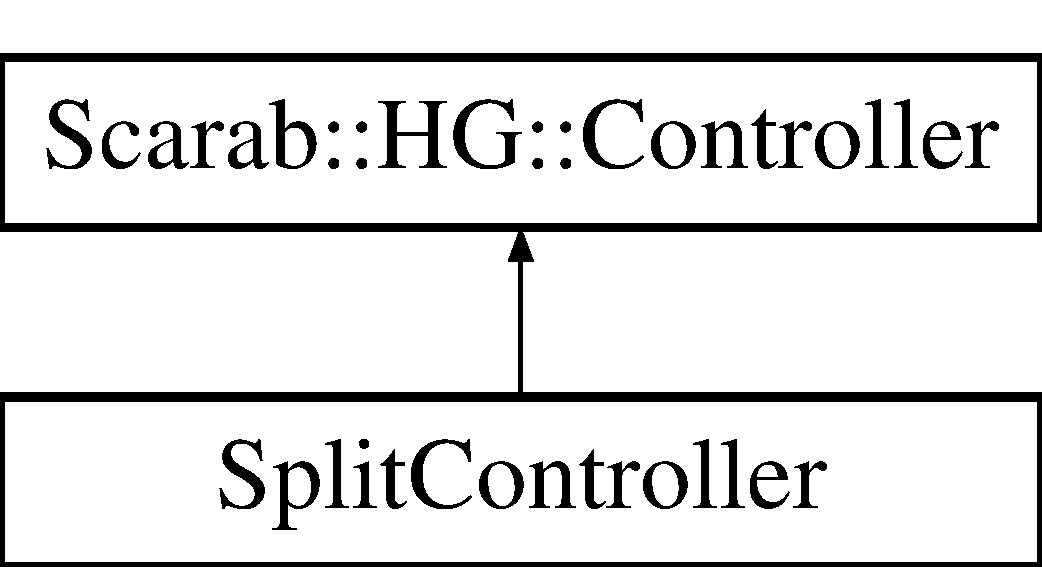
\includegraphics[height=2cm]{classSplitController}
\end{center}
\end{figure}
\subsection*{Public Member Functions}
\begin{DoxyCompactItemize}
\item 
\hypertarget{classSplitController_a511e733b586a24c2cad5ba16a6cb381b}{
{\bfseries SplitController} (const \hyperlink{classSubproblem}{Subproblem} \&s, const \hyperlink{classForestLattice}{ForestLattice} \&l, bool two\_\-classes)}
\label{classSplitController_a511e733b586a24c2cad5ba16a6cb381b}

\item 
\hypertarget{classSplitController_ac01bf4220c60c35f6862160dc7fcacc7}{
int {\bfseries project\_\-word} (int w) const }
\label{classSplitController_ac01bf4220c60c35f6862160dc7fcacc7}

\item 
\hypertarget{classSplitController_a272757bbbfaa9af9d2ee2262b03ef131}{
int {\bfseries size} () const }
\label{classSplitController_a272757bbbfaa9af9d2ee2262b03ef131}

\item 
\hypertarget{classSplitController_ad2aeeafdc31d48526be15a1b1a2e9931}{
int {\bfseries dim} () const }
\label{classSplitController_ad2aeeafdc31d48526be15a1b1a2e9931}

\item 
\hypertarget{classSplitController_a6ac91d8fd5fef735c6572c420a05bda4}{
void {\bfseries initialize\_\-hypotheses} (const \hyperlink{classScarab_1_1HG_1_1Hypernode}{Hypernode} \&node, vector$<$ \hyperlink{structScarab_1_1HG_1_1Hypothesis}{Hypothesis} $\ast$ $>$ \&hyps, vector$<$ double $>$ \&scores) const }
\label{classSplitController_a6ac91d8fd5fef735c6572c420a05bda4}

\item 
\hypertarget{classSplitController_a58e535837326d733c98a193f2c7584c6}{
void {\bfseries initialize\_\-out\_\-root} (vector$<$ \hyperlink{structScarab_1_1HG_1_1Hypothesis}{Hypothesis} $\ast$ $>$ \&hyps, vector$<$ double $>$ \&scores) const }
\label{classSplitController_a58e535837326d733c98a193f2c7584c6}

\item 
\hypertarget{classSplitController_a2138b9bac43d19896f2bff71a619e9af}{
double {\bfseries find\_\-best} (vector$<$ \hyperlink{structScarab_1_1HG_1_1Hypothesis}{Hypothesis} $\ast$ $>$ \&root\_\-hyps, vector$<$ double $>$ \&scores, \hyperlink{structScarab_1_1HG_1_1Hypothesis}{Hypothesis} \&best\_\-hyp) const }
\label{classSplitController_a2138b9bac43d19896f2bff71a619e9af}

\end{DoxyCompactItemize}


The documentation for this class was generated from the following file:\begin{DoxyCompactItemize}
\item 
trans\_\-decode/Decode.cpp\end{DoxyCompactItemize}

\hypertarget{classSplitHeuristic}{
\section{SplitHeuristic Class Reference}
\label{classSplitHeuristic}\index{SplitHeuristic@{SplitHeuristic}}
}
Inheritance diagram for SplitHeuristic:\begin{figure}[H]
\begin{center}
\leavevmode
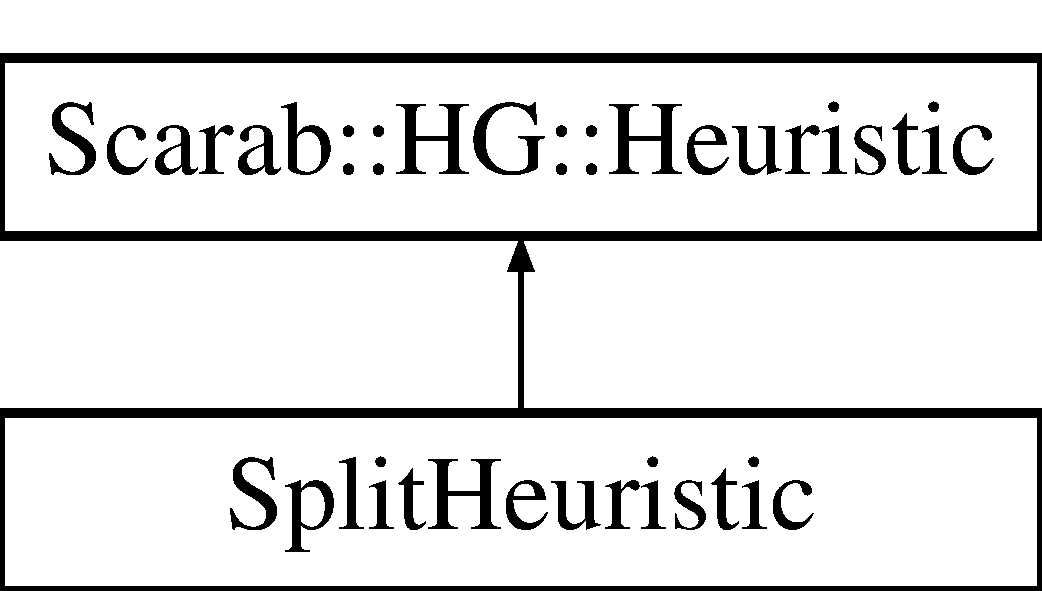
\includegraphics[height=2cm]{classSplitHeuristic}
\end{center}
\end{figure}
\subsection*{Public Member Functions}
\begin{DoxyCompactItemize}
\item 
\hypertarget{classSplitHeuristic_a8f58e4a4833f73460e2b2fb9c38448f1}{
{\bfseries SplitHeuristic} (const \hyperlink{classCache}{Cache}$<$ \hyperlink{classScarab_1_1HG_1_1Hypernode}{Hypernode}, \hyperlink{classScarab_1_1HG_1_1BestHyp}{BestHyp} $>$ \&outside\_\-scores, \hyperlink{classCache}{Cache}$<$ \hyperlink{classScarab_1_1HG_1_1Hyperedge}{Hyperedge}, vector$<$ \hyperlink{classScarab_1_1HG_1_1BestHyp}{BestHyp} $>$ $>$ \&outside\_\-edge\_\-scores)}
\label{classSplitHeuristic_a8f58e4a4833f73460e2b2fb9c38448f1}

\item 
\hypertarget{classSplitHeuristic_a0080cc4428de2635263f31d7931c3066}{
int {\bfseries lower\_\-id} (const \hyperlink{structScarab_1_1HG_1_1Hypothesis}{Hypothesis} \&hyp) const }
\label{classSplitHeuristic_a0080cc4428de2635263f31d7931c3066}

\item 
\hypertarget{classSplitHeuristic_a7117c99ce380835ed38aa02f82f8a04e}{
bool {\bfseries has\_\-value} (const \hyperlink{structScarab_1_1HG_1_1Location}{Location} \&l, const \hyperlink{structScarab_1_1HG_1_1Hypothesis}{Hypothesis} \&hyp) const }
\label{classSplitHeuristic_a7117c99ce380835ed38aa02f82f8a04e}

\item 
\hypertarget{classSplitHeuristic_ab64ec7cde28b49828bcde1ad97862cc2}{
double {\bfseries get\_\-value} (const \hyperlink{structScarab_1_1HG_1_1Location}{Location} \&l, const \hyperlink{structScarab_1_1HG_1_1Hypothesis}{Hypothesis} \&hyp) const }
\label{classSplitHeuristic_ab64ec7cde28b49828bcde1ad97862cc2}

\end{DoxyCompactItemize}


The documentation for this class was generated from the following file:\begin{DoxyCompactItemize}
\item 
trans\_\-decode/Decode.cpp\end{DoxyCompactItemize}

\hypertarget{classgraph_1_1State}{
\section{graph::State Class Reference}
\label{classgraph_1_1State}\index{graph::State@{graph::State}}
}
\subsection*{Public Member Functions}
\begin{DoxyCompactItemize}
\item 
\hypertarget{classgraph_1_1State_a6adb7a9d2cd11d5be8e4f2b66e0a8be9}{
{\bfseries State} (const \hyperlink{classgraph_1_1State}{State} \&from)}
\label{classgraph_1_1State_a6adb7a9d2cd11d5be8e4f2b66e0a8be9}

\item 
\hypertarget{classgraph_1_1State_ae565f2fef5dc685a53d67b1449672d53}{
\hyperlink{classgraph_1_1State}{State} \& {\bfseries operator=} (const \hyperlink{classgraph_1_1State}{State} \&from)}
\label{classgraph_1_1State_ae565f2fef5dc685a53d67b1449672d53}

\item 
\hypertarget{classgraph_1_1State_a6949f7b56f23e1f22f6ffd92cb22a339}{
const ::google::protobuf::UnknownFieldSet \& {\bfseries unknown\_\-fields} () const }
\label{classgraph_1_1State_a6949f7b56f23e1f22f6ffd92cb22a339}

\item 
\hypertarget{classgraph_1_1State_a7449bfa3aeb18cae2903328f38734898}{
inline::google::protobuf::UnknownFieldSet $\ast$ {\bfseries mutable\_\-unknown\_\-fields} ()}
\label{classgraph_1_1State_a7449bfa3aeb18cae2903328f38734898}

\item 
\hypertarget{classgraph_1_1State_a849d6b8710f8f11340460166556af6a4}{
void {\bfseries Swap} (\hyperlink{classgraph_1_1State}{State} $\ast$other)}
\label{classgraph_1_1State_a849d6b8710f8f11340460166556af6a4}

\item 
\hypertarget{classgraph_1_1State_a86924d60268be8025b78b75764061494}{
\hyperlink{classgraph_1_1State}{State} $\ast$ {\bfseries New} () const }
\label{classgraph_1_1State_a86924d60268be8025b78b75764061494}

\item 
\hypertarget{classgraph_1_1State_a4d9ab6623e196805d8980da3c86c282e}{
void {\bfseries CopyFrom} (const ::google::protobuf::Message \&from)}
\label{classgraph_1_1State_a4d9ab6623e196805d8980da3c86c282e}

\item 
\hypertarget{classgraph_1_1State_a30c21580da4c4a0aabb377ea18faa6ca}{
void {\bfseries MergeFrom} (const ::google::protobuf::Message \&from)}
\label{classgraph_1_1State_a30c21580da4c4a0aabb377ea18faa6ca}

\item 
\hypertarget{classgraph_1_1State_abfbeda00609f734e2bd45532e3b64869}{
void {\bfseries CopyFrom} (const \hyperlink{classgraph_1_1State}{State} \&from)}
\label{classgraph_1_1State_abfbeda00609f734e2bd45532e3b64869}

\item 
\hypertarget{classgraph_1_1State_ab523b1c4f8d71da48e446e3884d6027a}{
void {\bfseries MergeFrom} (const \hyperlink{classgraph_1_1State}{State} \&from)}
\label{classgraph_1_1State_ab523b1c4f8d71da48e446e3884d6027a}

\item 
\hypertarget{classgraph_1_1State_a7e43bad443bae237f2d8f3da129c29b2}{
void {\bfseries Clear} ()}
\label{classgraph_1_1State_a7e43bad443bae237f2d8f3da129c29b2}

\item 
\hypertarget{classgraph_1_1State_ab4efc2c78ba99b00f8fdab324191dc82}{
bool {\bfseries IsInitialized} () const }
\label{classgraph_1_1State_ab4efc2c78ba99b00f8fdab324191dc82}

\item 
\hypertarget{classgraph_1_1State_a22390019514703125f352bad7f38e023}{
int {\bfseries ByteSize} () const }
\label{classgraph_1_1State_a22390019514703125f352bad7f38e023}

\item 
\hypertarget{classgraph_1_1State_a8d96e8a53c415c86a55186c99f6f09e2}{
bool {\bfseries MergePartialFromCodedStream} (::google::protobuf::io::CodedInputStream $\ast$input)}
\label{classgraph_1_1State_a8d96e8a53c415c86a55186c99f6f09e2}

\item 
\hypertarget{classgraph_1_1State_a33dde93606b7e7e3f68f17fa39c9600c}{
void {\bfseries SerializeWithCachedSizes} (::google::protobuf::io::CodedOutputStream $\ast$output) const }
\label{classgraph_1_1State_a33dde93606b7e7e3f68f17fa39c9600c}

\item 
\hypertarget{classgraph_1_1State_a5c2538044c4523a9bdaa9bcdecc66045}{
::google::protobuf::uint8 $\ast$ {\bfseries SerializeWithCachedSizesToArray} (::google::protobuf::uint8 $\ast$output) const }
\label{classgraph_1_1State_a5c2538044c4523a9bdaa9bcdecc66045}

\item 
\hypertarget{classgraph_1_1State_a3c945006c8e96f17c55ad4c6461bf559}{
int {\bfseries GetCachedSize} () const }
\label{classgraph_1_1State_a3c945006c8e96f17c55ad4c6461bf559}

\item 
\hypertarget{classgraph_1_1State_a510521753605235c819924fe49a8b7ec}{
::google::protobuf::Metadata {\bfseries GetMetadata} () const }
\label{classgraph_1_1State_a510521753605235c819924fe49a8b7ec}

\item 
\hypertarget{classgraph_1_1State_a2669d4177d26e3feac6d3dfb58d8c10f}{
bool {\bfseries has\_\-id} () const }
\label{classgraph_1_1State_a2669d4177d26e3feac6d3dfb58d8c10f}

\item 
\hypertarget{classgraph_1_1State_af5d8971127b8388c60d286a26551bf93}{
void {\bfseries clear\_\-id} ()}
\label{classgraph_1_1State_af5d8971127b8388c60d286a26551bf93}

\item 
\hypertarget{classgraph_1_1State_a416aab28308b055a2e54e7fc85af56bd}{
inline::google::protobuf::int32 {\bfseries id} () const }
\label{classgraph_1_1State_a416aab28308b055a2e54e7fc85af56bd}

\item 
\hypertarget{classgraph_1_1State_a6c8d8623291ab2af0593785d73a5c52d}{
void {\bfseries set\_\-id} (::google::protobuf::int32 value)}
\label{classgraph_1_1State_a6c8d8623291ab2af0593785d73a5c52d}

\item 
\hypertarget{classgraph_1_1State_a9ec12f5818b8bf307eaf25cadb81394b}{
bool {\bfseries has\_\-label} () const }
\label{classgraph_1_1State_a9ec12f5818b8bf307eaf25cadb81394b}

\item 
\hypertarget{classgraph_1_1State_addbbc517bb046fc9e01888084a0c210d}{
void {\bfseries clear\_\-label} ()}
\label{classgraph_1_1State_addbbc517bb046fc9e01888084a0c210d}

\item 
\hypertarget{classgraph_1_1State_a0357428ad565c96779a7c48056cd1add}{
const ::std::string \& {\bfseries label} () const }
\label{classgraph_1_1State_a0357428ad565c96779a7c48056cd1add}

\item 
\hypertarget{classgraph_1_1State_a47942a01a50058ffe3dc0727905e9716}{
void {\bfseries set\_\-label} (const ::std::string \&value)}
\label{classgraph_1_1State_a47942a01a50058ffe3dc0727905e9716}

\item 
\hypertarget{classgraph_1_1State_a9cd3283f813138b76481ca78732137ce}{
void {\bfseries set\_\-label} (const char $\ast$value)}
\label{classgraph_1_1State_a9cd3283f813138b76481ca78732137ce}

\item 
\hypertarget{classgraph_1_1State_a625e53965b650ff0c0ee33af336a95f7}{
void {\bfseries set\_\-label} (const char $\ast$value, size\_\-t size)}
\label{classgraph_1_1State_a625e53965b650ff0c0ee33af336a95f7}

\item 
\hypertarget{classgraph_1_1State_aebe2f189ede79c89a46de5c86be0daa1}{
inline::std::string $\ast$ {\bfseries mutable\_\-label} ()}
\label{classgraph_1_1State_aebe2f189ede79c89a46de5c86be0daa1}

\item 
\hypertarget{classgraph_1_1State_a8548defb5e484193d98b376d116c3d81}{
inline::std::string $\ast$ {\bfseries release\_\-label} ()}
\label{classgraph_1_1State_a8548defb5e484193d98b376d116c3d81}

\item 
\hypertarget{classgraph_1_1State_adbd7ef24b794167795d267dfbd1d0646}{
{\bfseries State} (const \hyperlink{classgraph_1_1State}{State} \&from)}
\label{classgraph_1_1State_adbd7ef24b794167795d267dfbd1d0646}

\item 
\hypertarget{classgraph_1_1State_ae565f2fef5dc685a53d67b1449672d53}{
\hyperlink{classgraph_1_1State}{State} \& {\bfseries operator=} (const \hyperlink{classgraph_1_1State}{State} \&from)}
\label{classgraph_1_1State_ae565f2fef5dc685a53d67b1449672d53}

\item 
\hypertarget{classgraph_1_1State_a6949f7b56f23e1f22f6ffd92cb22a339}{
const ::google::protobuf::UnknownFieldSet \& {\bfseries unknown\_\-fields} () const }
\label{classgraph_1_1State_a6949f7b56f23e1f22f6ffd92cb22a339}

\item 
\hypertarget{classgraph_1_1State_a7449bfa3aeb18cae2903328f38734898}{
inline::google::protobuf::UnknownFieldSet $\ast$ {\bfseries mutable\_\-unknown\_\-fields} ()}
\label{classgraph_1_1State_a7449bfa3aeb18cae2903328f38734898}

\item 
\hypertarget{classgraph_1_1State_affd9e019264a3a2416563d91dbed1f27}{
void {\bfseries Swap} (\hyperlink{classgraph_1_1State}{State} $\ast$other)}
\label{classgraph_1_1State_affd9e019264a3a2416563d91dbed1f27}

\item 
\hypertarget{classgraph_1_1State_a28b26e430542a30cfe3b79a0b86eacb2}{
\hyperlink{classgraph_1_1State}{State} $\ast$ {\bfseries New} () const }
\label{classgraph_1_1State_a28b26e430542a30cfe3b79a0b86eacb2}

\item 
\hypertarget{classgraph_1_1State_a9f329c3d5f8b4d2e42c7a7b8e9b2a5e6}{
void {\bfseries CopyFrom} (const ::google::protobuf::Message \&from)}
\label{classgraph_1_1State_a9f329c3d5f8b4d2e42c7a7b8e9b2a5e6}

\item 
\hypertarget{classgraph_1_1State_a3f0b1f20bac33c7254938c2e4dc44961}{
void {\bfseries MergeFrom} (const ::google::protobuf::Message \&from)}
\label{classgraph_1_1State_a3f0b1f20bac33c7254938c2e4dc44961}

\item 
\hypertarget{classgraph_1_1State_a2e62ade5c5af34b509befbbb2c36afd3}{
void {\bfseries CopyFrom} (const \hyperlink{classgraph_1_1State}{State} \&from)}
\label{classgraph_1_1State_a2e62ade5c5af34b509befbbb2c36afd3}

\item 
\hypertarget{classgraph_1_1State_a696753acbfc23dc59a3a4f47fd99b615}{
void {\bfseries MergeFrom} (const \hyperlink{classgraph_1_1State}{State} \&from)}
\label{classgraph_1_1State_a696753acbfc23dc59a3a4f47fd99b615}

\item 
\hypertarget{classgraph_1_1State_a20caa4e8b3584fb112bfc2b9a8e082ff}{
void {\bfseries Clear} ()}
\label{classgraph_1_1State_a20caa4e8b3584fb112bfc2b9a8e082ff}

\item 
\hypertarget{classgraph_1_1State_a01736d44a021a0bbc28676c35de6339d}{
bool {\bfseries IsInitialized} () const }
\label{classgraph_1_1State_a01736d44a021a0bbc28676c35de6339d}

\item 
\hypertarget{classgraph_1_1State_a89767644e0b92a1be04e504b35504bbc}{
int {\bfseries ByteSize} () const }
\label{classgraph_1_1State_a89767644e0b92a1be04e504b35504bbc}

\item 
\hypertarget{classgraph_1_1State_ae0c84f0786cb0690d7e473a718a3365d}{
bool {\bfseries MergePartialFromCodedStream} (::google::protobuf::io::CodedInputStream $\ast$input)}
\label{classgraph_1_1State_ae0c84f0786cb0690d7e473a718a3365d}

\item 
\hypertarget{classgraph_1_1State_a8261a94d9575d04e9dde511a2e1e16ce}{
void {\bfseries SerializeWithCachedSizes} (::google::protobuf::io::CodedOutputStream $\ast$output) const }
\label{classgraph_1_1State_a8261a94d9575d04e9dde511a2e1e16ce}

\item 
\hypertarget{classgraph_1_1State_a9311fff53a672da2c9709ad5f90ff092}{
::google::protobuf::uint8 $\ast$ {\bfseries SerializeWithCachedSizesToArray} (::google::protobuf::uint8 $\ast$output) const }
\label{classgraph_1_1State_a9311fff53a672da2c9709ad5f90ff092}

\item 
\hypertarget{classgraph_1_1State_a3c945006c8e96f17c55ad4c6461bf559}{
int {\bfseries GetCachedSize} () const }
\label{classgraph_1_1State_a3c945006c8e96f17c55ad4c6461bf559}

\item 
\hypertarget{classgraph_1_1State_af6574e950b5691fba98109d1c5a797e9}{
::google::protobuf::Metadata {\bfseries GetMetadata} () const }
\label{classgraph_1_1State_af6574e950b5691fba98109d1c5a797e9}

\item 
\hypertarget{classgraph_1_1State_a68a4cdaa1fdd3c9efa19908182efe1d4}{
bool {\bfseries has\_\-id} () const }
\label{classgraph_1_1State_a68a4cdaa1fdd3c9efa19908182efe1d4}

\item 
\hypertarget{classgraph_1_1State_ae1a090d3c77ac4080062d6397331be4f}{
void {\bfseries clear\_\-id} ()}
\label{classgraph_1_1State_ae1a090d3c77ac4080062d6397331be4f}

\item 
\hypertarget{classgraph_1_1State_a7e1ceeb0ab170c31bdc0a723036f5da3}{
inline::google::protobuf::int32 {\bfseries id} () const }
\label{classgraph_1_1State_a7e1ceeb0ab170c31bdc0a723036f5da3}

\item 
\hypertarget{classgraph_1_1State_ae08cae292bbbcf35ddc24ae7e7e39eda}{
void {\bfseries set\_\-id} (::google::protobuf::int32 value)}
\label{classgraph_1_1State_ae08cae292bbbcf35ddc24ae7e7e39eda}

\item 
\hypertarget{classgraph_1_1State_af5d76492e6f23b161ea418bd0191ea48}{
bool {\bfseries has\_\-label} () const }
\label{classgraph_1_1State_af5d76492e6f23b161ea418bd0191ea48}

\item 
\hypertarget{classgraph_1_1State_aa20bd8660731de966ba650d14c7ed353}{
void {\bfseries clear\_\-label} ()}
\label{classgraph_1_1State_aa20bd8660731de966ba650d14c7ed353}

\item 
\hypertarget{classgraph_1_1State_a574d6c801f38a0f41c222cf8f5f5a676}{
const ::std::string \& {\bfseries label} () const }
\label{classgraph_1_1State_a574d6c801f38a0f41c222cf8f5f5a676}

\item 
\hypertarget{classgraph_1_1State_aafc8a32bff5a6e4b8702d00b0963e12d}{
void {\bfseries set\_\-label} (const ::std::string \&value)}
\label{classgraph_1_1State_aafc8a32bff5a6e4b8702d00b0963e12d}

\item 
\hypertarget{classgraph_1_1State_a501eea62783e326dcabf304efe3776e6}{
void {\bfseries set\_\-label} (const char $\ast$value)}
\label{classgraph_1_1State_a501eea62783e326dcabf304efe3776e6}

\item 
\hypertarget{classgraph_1_1State_a429836f891cab177ebbc26b4631c554a}{
void {\bfseries set\_\-label} (const char $\ast$value, size\_\-t size)}
\label{classgraph_1_1State_a429836f891cab177ebbc26b4631c554a}

\item 
\hypertarget{classgraph_1_1State_aaab551134a99085aae249d9775dd5669}{
inline::std::string $\ast$ {\bfseries mutable\_\-label} ()}
\label{classgraph_1_1State_aaab551134a99085aae249d9775dd5669}

\item 
\hypertarget{classgraph_1_1State_ac45e9075ffe1302d36974886e4d725f3}{
inline::std::string $\ast$ {\bfseries release\_\-label} ()}
\label{classgraph_1_1State_ac45e9075ffe1302d36974886e4d725f3}

\end{DoxyCompactItemize}
\subsection*{Static Public Member Functions}
\begin{DoxyCompactItemize}
\item 
\hypertarget{classgraph_1_1State_a84099504e494d0d9ba226d60bd8e5db7}{
static const ::google::protobuf::Descriptor $\ast$ {\bfseries descriptor} ()}
\label{classgraph_1_1State_a84099504e494d0d9ba226d60bd8e5db7}

\item 
\hypertarget{classgraph_1_1State_a3b976f5020643cda46f45404a5838acf}{
static const \hyperlink{classgraph_1_1State}{State} \& {\bfseries default\_\-instance} ()}
\label{classgraph_1_1State_a3b976f5020643cda46f45404a5838acf}

\item 
\hypertarget{classgraph_1_1State_a3e8f14326a5b160291b2dc219270d685}{
static const ::google::protobuf::Descriptor $\ast$ {\bfseries descriptor} ()}
\label{classgraph_1_1State_a3e8f14326a5b160291b2dc219270d685}

\item 
\hypertarget{classgraph_1_1State_a585b25fdad9a4a8fccbab2d0274ce292}{
static const \hyperlink{classgraph_1_1State}{State} \& {\bfseries default\_\-instance} ()}
\label{classgraph_1_1State_a585b25fdad9a4a8fccbab2d0274ce292}

\end{DoxyCompactItemize}
\subsection*{Static Public Attributes}
\begin{DoxyCompactItemize}
\item 
\hypertarget{classgraph_1_1State_a150e9e7c58dd46aaf1dd05cddf8bbb96}{
static const int {\bfseries kIdFieldNumber} = 1}
\label{classgraph_1_1State_a150e9e7c58dd46aaf1dd05cddf8bbb96}

\item 
\hypertarget{classgraph_1_1State_a47c9ea89be631c1a5135c0b2d89a9ee4}{
static const int {\bfseries kLabelFieldNumber} = 2}
\label{classgraph_1_1State_a47c9ea89be631c1a5135c0b2d89a9ee4}

\end{DoxyCompactItemize}
\subsection*{Friends}
\begin{DoxyCompactItemize}
\item 
\hypertarget{classgraph_1_1State_a7c7daba01236a33140ac99dfb4a21f58}{
void {\bfseries protobuf\_\-AddDesc\_\-mrf\_\-2eproto} ()}
\label{classgraph_1_1State_a7c7daba01236a33140ac99dfb4a21f58}

\item 
\hypertarget{classgraph_1_1State_aef3db81db7837e30d95a050165bc180f}{
void {\bfseries protobuf\_\-AssignDesc\_\-mrf\_\-2eproto} ()}
\label{classgraph_1_1State_aef3db81db7837e30d95a050165bc180f}

\item 
\hypertarget{classgraph_1_1State_a84e801a5b8303ac698fb7040b250e3d1}{
void {\bfseries protobuf\_\-ShutdownFile\_\-mrf\_\-2eproto} ()}
\label{classgraph_1_1State_a84e801a5b8303ac698fb7040b250e3d1}

\item 
\hypertarget{classgraph_1_1State_a7c7daba01236a33140ac99dfb4a21f58}{
void {\bfseries protobuf\_\-AddDesc\_\-mrf\_\-2eproto} ()}
\label{classgraph_1_1State_a7c7daba01236a33140ac99dfb4a21f58}

\item 
\hypertarget{classgraph_1_1State_aef3db81db7837e30d95a050165bc180f}{
void {\bfseries protobuf\_\-AssignDesc\_\-mrf\_\-2eproto} ()}
\label{classgraph_1_1State_aef3db81db7837e30d95a050165bc180f}

\item 
\hypertarget{classgraph_1_1State_a84e801a5b8303ac698fb7040b250e3d1}{
void {\bfseries protobuf\_\-ShutdownFile\_\-mrf\_\-2eproto} ()}
\label{classgraph_1_1State_a84e801a5b8303ac698fb7040b250e3d1}

\end{DoxyCompactItemize}


The documentation for this class was generated from the following files:\begin{DoxyCompactItemize}
\item 
interfaces/graph/gen-\/cpp/mrf.pb.h\item 
interfaces/graph/gen-\/py/mrf.pb.h\item 
interfaces/graph/gen-\/cpp/mrf.pb.cc\item 
interfaces/graph/gen-\/py/mrf.pb.cc\end{DoxyCompactItemize}

\hypertarget{structState}{
\section{State Struct Reference}
\label{structState}\index{State@{State}}
}
\subsection*{Public Member Functions}
\begin{DoxyCompactItemize}
\item 
\hypertarget{structState_aa536880320a9aff707fb1e6aab3f58d4}{
{\bfseries State} (int id\_\-, string label\_\-)}
\label{structState_aa536880320a9aff707fb1e6aab3f58d4}

\item 
\hypertarget{structState_aea25c6702974d1ac86358b4ba96d7891}{
int {\bfseries id} () const }
\label{structState_aea25c6702974d1ac86358b4ba96d7891}

\item 
\hypertarget{structState_a2809d0a34cd576cc5daaa7a6d0ffb2b5}{
string {\bfseries label} () const }
\label{structState_a2809d0a34cd576cc5daaa7a6d0ffb2b5}

\item 
\hypertarget{structState_a6687a56382a022034927ba43aad39524}{
bool {\bfseries operator==} (const \hyperlink{structState}{State} \&other) const }
\label{structState_a6687a56382a022034927ba43aad39524}

\end{DoxyCompactItemize}
\subsection*{Public Attributes}
\begin{DoxyCompactItemize}
\item 
\hypertarget{structState_ae0482e3d4b3db023647833efd344831a}{
int {\bfseries \_\-id}}
\label{structState_ae0482e3d4b3db023647833efd344831a}

\item 
\hypertarget{structState_a1bf6100c59d50bc94ba781230a85a2e5}{
string {\bfseries \_\-label}}
\label{structState_a1bf6100c59d50bc94ba781230a85a2e5}

\end{DoxyCompactItemize}


The documentation for this struct was generated from the following file:\begin{DoxyCompactItemize}
\item 
optimization/MRF.h\end{DoxyCompactItemize}

\hypertarget{structScarab_1_1HG_1_1State}{
\section{Scarab::HG::State Struct Reference}
\label{structScarab_1_1HG_1_1State}\index{Scarab::HG::State@{Scarab::HG::State}}
}
\subsection*{Public Member Functions}
\begin{DoxyCompactItemize}
\item 
\hypertarget{structScarab_1_1HG_1_1State_a61592030e999341da1e674274db11307}{
{\bfseries State} (const vector$<$ int $>$ \&ids, uint dim)}
\label{structScarab_1_1HG_1_1State_a61592030e999341da1e674274db11307}

\item 
\hypertarget{structScarab_1_1HG_1_1State_a6597ae0951c6d0c9146ae6bd5b91b52f}{
\hyperlink{structScarab_1_1HG_1_1State}{State} {\bfseries project} (int split, int down\_\-to) const }
\label{structScarab_1_1HG_1_1State_a6597ae0951c6d0c9146ae6bd5b91b52f}

\item 
\hypertarget{structScarab_1_1HG_1_1State_ac7f5641edb1dd813dcac3b76be28d305}{
int {\bfseries id} () const }
\label{structScarab_1_1HG_1_1State_ac7f5641edb1dd813dcac3b76be28d305}

\item 
\hypertarget{structScarab_1_1HG_1_1State_a17d205eca9f3be9c01c7d41e3fe4d809}{
bool {\bfseries operator==} (const \hyperlink{structScarab_1_1HG_1_1State}{State} \&other) const }
\label{structScarab_1_1HG_1_1State_a17d205eca9f3be9c01c7d41e3fe4d809}

\item 
\hypertarget{structScarab_1_1HG_1_1State_acd8ef3e5bd73ec5034de0d70f2bb2492}{
bool {\bfseries compatible} (const \hyperlink{structScarab_1_1HG_1_1State}{State} \&other) const }
\label{structScarab_1_1HG_1_1State_acd8ef3e5bd73ec5034de0d70f2bb2492}

\item 
\hypertarget{structScarab_1_1HG_1_1State_abadb936b551a91d952af74b3bfc7d43d}{
bool {\bfseries operator$<$} (const \hyperlink{structScarab_1_1HG_1_1State}{State} \&other) const }
\label{structScarab_1_1HG_1_1State_abadb936b551a91d952af74b3bfc7d43d}

\item 
\hypertarget{structScarab_1_1HG_1_1State_afc65eeacc345b5396a673e4328cccc11}{
int {\bfseries possible\_\-states} () const }
\label{structScarab_1_1HG_1_1State_afc65eeacc345b5396a673e4328cccc11}

\end{DoxyCompactItemize}
\subsection*{Public Attributes}
\begin{DoxyCompactItemize}
\item 
\hypertarget{structScarab_1_1HG_1_1State_a1c516b546a5e3de3a5f9bb8f39a3cf20}{
vector$<$ int $>$ {\bfseries \_\-state}}
\label{structScarab_1_1HG_1_1State_a1c516b546a5e3de3a5f9bb8f39a3cf20}

\end{DoxyCompactItemize}
\subsection*{Protected Attributes}
\begin{DoxyCompactItemize}
\item 
\hypertarget{structScarab_1_1HG_1_1State_ae3d755b161845bd295deae4096d4c9f8}{
uint {\bfseries \_\-dim}}
\label{structScarab_1_1HG_1_1State_ae3d755b161845bd295deae4096d4c9f8}

\end{DoxyCompactItemize}
\subsection*{Friends}
\begin{DoxyCompactItemize}
\item 
\hypertarget{structScarab_1_1HG_1_1State_a353ffb342165fcaec0e812d0288fc329}{
ostream \& {\bfseries operator$<$$<$} (ostream \&output, const \hyperlink{structScarab_1_1HG_1_1State}{State} \&p)}
\label{structScarab_1_1HG_1_1State_a353ffb342165fcaec0e812d0288fc329}

\end{DoxyCompactItemize}


The documentation for this struct was generated from the following file:\begin{DoxyCompactItemize}
\item 
hypergraph/Hypothesis.h\end{DoxyCompactItemize}

\hypertarget{classStoreCache}{
\section{StoreCache$<$ C, V $>$ Class Template Reference}
\label{classStoreCache}\index{StoreCache@{StoreCache}}
}
\subsection*{Public Member Functions}
\begin{DoxyCompactItemize}
\item 
\hypertarget{classStoreCache_adeb02113caf8141430705ec5bab08a54}{
{\bfseries StoreCache} (int size)}
\label{classStoreCache_adeb02113caf8141430705ec5bab08a54}

\item 
\hypertarget{classStoreCache_a5aaafba803337cf3547159a6ac70a0ab}{
void {\bfseries resize} (int size)}
\label{classStoreCache_a5aaafba803337cf3547159a6ac70a0ab}

\item 
\hypertarget{classStoreCache_aa4673d48544458b6b05770fe5970d961}{
int {\bfseries size} () const }
\label{classStoreCache_aa4673d48544458b6b05770fe5970d961}

\item 
\hypertarget{classStoreCache_a455dbf75e40300745b354fdcc039279a}{
V {\bfseries get\_\-value} (const C \&edge) const }
\label{classStoreCache_a455dbf75e40300745b354fdcc039279a}

\item 
\hypertarget{classStoreCache_a23309f685f0ba18912dcc2e8643de932}{
void {\bfseries set\_\-value} (const C \&edge, V val)}
\label{classStoreCache_a23309f685f0ba18912dcc2e8643de932}

\item 
\hypertarget{classStoreCache_aa1289fedb472667dfa926c1e00f22b95}{
bool {\bfseries has\_\-key} (const C \&edge) const }
\label{classStoreCache_aa1289fedb472667dfa926c1e00f22b95}

\item 
\hypertarget{classStoreCache_ad358ce23080bb52db50a55db583f1bba}{
bool {\bfseries has\_\-key} (int k) const }
\label{classStoreCache_ad358ce23080bb52db50a55db583f1bba}

\end{DoxyCompactItemize}
\subsection*{Public Attributes}
\begin{DoxyCompactItemize}
\item 
\hypertarget{classStoreCache_a99393733357e04fe79cf703d3f4d8f44}{
vector$<$ V $>$ {\bfseries store}}
\label{classStoreCache_a99393733357e04fe79cf703d3f4d8f44}

\item 
\hypertarget{classStoreCache_a0df08d5576ce34c4a8fd4f7428fd9ad3}{
vector$<$ C $>$ {\bfseries full\_\-keys}}
\label{classStoreCache_a0df08d5576ce34c4a8fd4f7428fd9ad3}

\item 
\hypertarget{classStoreCache_acdfad2c43fd63e37fbb818ce282f6493}{
vector$<$ bool $>$ {\bfseries has\_\-value}}
\label{classStoreCache_acdfad2c43fd63e37fbb818ce282f6493}

\end{DoxyCompactItemize}
\subsubsection*{template$<$class C, class V$>$ class StoreCache$<$ C, V $>$}



The documentation for this class was generated from the following file:\begin{DoxyCompactItemize}
\item 
hypergraph/EdgeCache.h\end{DoxyCompactItemize}

\hypertarget{classSubgradient}{
\section{Subgradient Class Reference}
\label{classSubgradient}\index{Subgradient@{Subgradient}}
}
\subsection*{Public Member Functions}
\begin{DoxyCompactItemize}
\item 
\hyperlink{classSubgradient_a2509e39964e1280532fd4994b3d747ce}{Subgradient} (\hyperlink{classSubgradientProducer}{SubgradientProducer} \&subgrad\_\-producer)
\item 
\hypertarget{classSubgradient_a183205851cdb362195baf914fb8d3ae0}{
void {\bfseries solve} (int example)}
\label{classSubgradient_a183205851cdb362195baf914fb8d3ae0}

\item 
bool \hyperlink{classSubgradient_a54907389766b702c467cf2ab20f8d051}{is\_\-stuck} () const 
\end{DoxyCompactItemize}


\subsection{Constructor \& Destructor Documentation}
\hypertarget{classSubgradient_a2509e39964e1280532fd4994b3d747ce}{
\index{Subgradient@{Subgradient}!Subgradient@{Subgradient}}
\index{Subgradient@{Subgradient}!Subgradient@{Subgradient}}
\subsubsection[{Subgradient}]{\setlength{\rightskip}{0pt plus 5cm}Subgradient::Subgradient ({\bf SubgradientProducer} \& {\em subgrad\_\-producer})\hspace{0.3cm}{\ttfamily  \mbox{[}inline\mbox{]}}}}
\label{classSubgradient_a2509e39964e1280532fd4994b3d747ce}

\begin{DoxyParams}{Parameters}
\item[{\em subgrad\_\-producer}]Gives the subgradient at the current position \end{DoxyParams}


\subsection{Member Function Documentation}
\hypertarget{classSubgradient_a54907389766b702c467cf2ab20f8d051}{
\index{Subgradient@{Subgradient}!is\_\-stuck@{is\_\-stuck}}
\index{is\_\-stuck@{is\_\-stuck}!Subgradient@{Subgradient}}
\subsubsection[{is\_\-stuck}]{\setlength{\rightskip}{0pt plus 5cm}bool Subgradient::is\_\-stuck () const\hspace{0.3cm}{\ttfamily  \mbox{[}inline\mbox{]}}}}
\label{classSubgradient_a54907389766b702c467cf2ab20f8d051}
As the optimization probably reached a fixed point

\begin{DoxyReturn}{Returns}
true when stuck 
\end{DoxyReturn}


The documentation for this class was generated from the following files:\begin{DoxyCompactItemize}
\item 
optimization/Subgradient.h\item 
optimization/Subgradient.cpp\end{DoxyCompactItemize}

\hypertarget{classSubgradientProducer}{
\section{SubgradientProducer Class Reference}
\label{classSubgradientProducer}\index{SubgradientProducer@{SubgradientProducer}}
}
Inheritance diagram for SubgradientProducer:\begin{figure}[H]
\begin{center}
\leavevmode
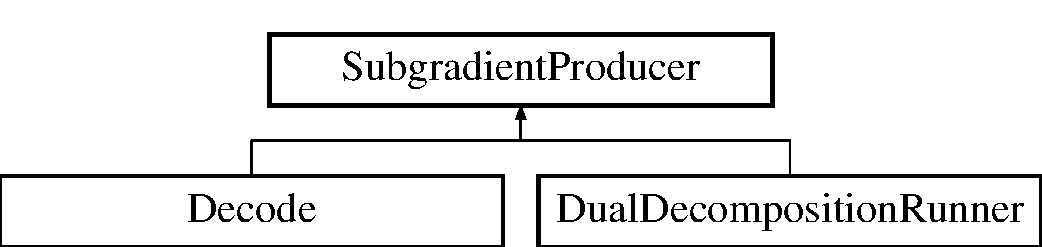
\includegraphics[height=2cm]{classSubgradientProducer}
\end{center}
\end{figure}
\subsection*{Public Member Functions}
\begin{DoxyCompactItemize}
\item 
\hypertarget{classSubgradientProducer_acea0e6ef35f9f3fd2f14872740471628}{
virtual void {\bfseries solve} (double \&primal, double \&dual, wvector \&, int, bool, bool \&)=0}
\label{classSubgradientProducer_acea0e6ef35f9f3fd2f14872740471628}

\item 
\hypertarget{classSubgradientProducer_a5b471526b337913722f56221b2461d89}{
virtual void {\bfseries update\_\-weights} (const wvector \&updates, wvector $\ast$weights)=0}
\label{classSubgradientProducer_a5b471526b337913722f56221b2461d89}

\end{DoxyCompactItemize}


The documentation for this class was generated from the following file:\begin{DoxyCompactItemize}
\item 
optimization/Subgradient.h\end{DoxyCompactItemize}

\hypertarget{classSubproblem}{
\section{Subproblem Class Reference}
\label{classSubproblem}\index{Subproblem@{Subproblem}}
}
\subsection*{Public Member Functions}
\begin{DoxyCompactItemize}
\item 
\hypertarget{classSubproblem_a1f76e6e7b079168299046c42e484c9cf}{
int {\bfseries overridden\_\-by} (int w) const }
\label{classSubproblem_a1f76e6e7b079168299046c42e484c9cf}

\item 
\hypertarget{classSubproblem_aba36ea76049a46e9ba1f0ac3ccec540a}{
void {\bfseries project} (int proj\_\-dim, vector$<$ int $>$ projection)}
\label{classSubproblem_aba36ea76049a46e9ba1f0ac3ccec540a}

\item 
\hypertarget{classSubproblem_a7c86b92cc388505602707376e52a0804}{
int {\bfseries project\_\-word} (int w) const }
\label{classSubproblem_a7c86b92cc388505602707376e52a0804}

\item 
\hypertarget{classSubproblem_a3f6d78f4567e70c35785d27a53a55490}{
void {\bfseries separate} (int w1, int w2)}
\label{classSubproblem_a3f6d78f4567e70c35785d27a53a55490}

\item 
\hypertarget{classSubproblem_a503126c48810484433fd6c3e428f6537}{
void {\bfseries projection\_\-with\_\-constraints} (int limit, int \&k, map$<$ int, set$<$ int $>$ $>$ \&constraints, vector$<$ int $>$ \&)}
\label{classSubproblem_a503126c48810484433fd6c3e428f6537}

\item 
\hypertarget{classSubproblem_a4c12e798de9d3e96d6935bd755f92a97}{
int {\bfseries best\_\-one} (int w1, int w2, int w3) const }
\label{classSubproblem_a4c12e798de9d3e96d6935bd755f92a97}

\item 
\hypertarget{classSubproblem_abf452bcac2a8a28adbdbffe402e64dde}{
int {\bfseries best\_\-two} (int w1, int w2, int w3) const }
\label{classSubproblem_abf452bcac2a8a28adbdbffe402e64dde}

\item 
\hypertarget{classSubproblem_a80e4996ec87d5c3501ef10abdd953260}{
double {\bfseries best\_\-score\_\-dim} (int w1, int d, int d2) const }
\label{classSubproblem_a80e4996ec87d5c3501ef10abdd953260}

\item 
\hypertarget{classSubproblem_a2e2a665cfdb9208f753eef143147d66c}{
double {\bfseries best\_\-score\_\-dim\_\-min} (int w1, vector$<$ int $>$ ds, vector$<$ int $>$ ds2) const }
\label{classSubproblem_a2e2a665cfdb9208f753eef143147d66c}

\item 
\hypertarget{classSubproblem_a2b43a2a68724d8eb624f6d81a7745b70}{
bool {\bfseries is\_\-new\_\-dim} (int w1, int d, int d2) const }
\label{classSubproblem_a2b43a2a68724d8eb624f6d81a7745b70}

\item 
\hypertarget{classSubproblem_a8359ae9db4d8a830d390312bc57eef6f}{
double {\bfseries best\_\-score} (int w1, int w2, int w3) const }
\label{classSubproblem_a8359ae9db4d8a830d390312bc57eef6f}

\item 
\hypertarget{classSubproblem_ae6b6a16e00079ebd5b56acbdfdaf3aab}{
{\bfseries Subproblem} (const \hyperlink{classForestLattice}{ForestLattice} $\ast$g, \hyperlink{classNgramCache}{NgramCache} $\ast$lm\_\-in, const \hyperlink{classGraphDecompose}{GraphDecompose} $\ast$gd\_\-in, const \hyperlink{classCache}{Cache}$<$ \hyperlink{classScarab_1_1Graph_1_1Graphnode}{Graphnode}, int $>$ \&word\_\-node\_\-cache\_\-in)}
\label{classSubproblem_ae6b6a16e00079ebd5b56acbdfdaf3aab}

\item 
\hypertarget{classSubproblem_adf6eb478907ed5c7c9f08a3cfcdfec76}{
void {\bfseries update\_\-weights} (vector$<$ int $>$ u\_\-pos, vector$<$ float $>$ u\_\-values, bool first)}
\label{classSubproblem_adf6eb478907ed5c7c9f08a3cfcdfec76}

\item 
\hypertarget{classSubproblem_a27c807a807f154ea28e7da7692466638}{
void {\bfseries solve} ()}
\label{classSubproblem_a27c807a807f154ea28e7da7692466638}

\item 
\hypertarget{classSubproblem_a8220595977ed219234d36dfadd0dde82}{
void {\bfseries initialize\_\-caches} ()}
\label{classSubproblem_a8220595977ed219234d36dfadd0dde82}

\item 
\hypertarget{classSubproblem_a9c57f3bd41e2788d9f393db8bbbe26ef}{
vector$<$ int $>$ {\bfseries get\_\-best\_\-nodes\_\-between} (int w1, int w2, bool first)}
\label{classSubproblem_a9c57f3bd41e2788d9f393db8bbbe26ef}

\item 
\hypertarget{classSubproblem_a3c426fd46fcacefc561b68f0fc111795}{
float {\bfseries get\_\-best\_\-bigram\_\-weight} (int w1, int w2, bool first)}
\label{classSubproblem_a3c426fd46fcacefc561b68f0fc111795}

\item 
\hypertarget{classSubproblem_adfba5511e1f004b989f7b2e03d998c4e}{
float {\bfseries primal\_\-score} (int word\mbox{[}$\,$\mbox{]}, int l)}
\label{classSubproblem_adfba5511e1f004b989f7b2e03d998c4e}

\item 
\hypertarget{classSubproblem_ab5e3b5e167561a79da1d815af120b6bd}{
double {\bfseries word\_\-prob} (int, int, int)}
\label{classSubproblem_ab5e3b5e167561a79da1d815af120b6bd}

\item 
\hypertarget{classSubproblem_acc456e9852f19058da2d884feec15679}{
double {\bfseries word\_\-backoff} (int)}
\label{classSubproblem_acc456e9852f19058da2d884feec15679}

\item 
\hypertarget{classSubproblem_afd0b98fea6ebb39ae5ad46d1010cb6a3}{
double {\bfseries word\_\-backoff\_\-two} (int i, int j)}
\label{classSubproblem_afd0b98fea6ebb39ae5ad46d1010cb6a3}

\item 
\hypertarget{classSubproblem_a32718cd109a52be59a7eecd3dc5f4c8a}{
double {\bfseries word\_\-prob\_\-reverse} (int, int, int)}
\label{classSubproblem_a32718cd109a52be59a7eecd3dc5f4c8a}

\item 
\hypertarget{classSubproblem_ab612e729dd11b5ac27ce9f67e0135c0a}{
double {\bfseries word\_\-prob\_\-bigram\_\-reverse} (int i, int j)}
\label{classSubproblem_ab612e729dd11b5ac27ce9f67e0135c0a}

\item 
\hypertarget{classSubproblem_a522f5f38fddff38424fe3958104a9612}{
int {\bfseries word\_\-bow\_\-reverse} (int i, int j, int k)}
\label{classSubproblem_a522f5f38fddff38424fe3958104a9612}

\item 
\hypertarget{classSubproblem_a1bce1ad18ee9c123677f39cccda7feb5}{
int {\bfseries word\_\-bow\_\-bigram\_\-reverse} (int i, int j)}
\label{classSubproblem_a1bce1ad18ee9c123677f39cccda7feb5}

\end{DoxyCompactItemize}
\subsection*{Public Attributes}
\begin{DoxyCompactItemize}
\item 
\hypertarget{classSubproblem_ab162552f8af9ee111227f6ec30b7a4f5}{
vector$<$ bool $>$ {\bfseries overridden}}
\label{classSubproblem_ab162552f8af9ee111227f6ec30b7a4f5}

\item 
\hypertarget{classSubproblem_aa981fb8aa661221937b3cd021d72c396}{
int {\bfseries projection\_\-dims}}
\label{classSubproblem_aa981fb8aa661221937b3cd021d72c396}

\end{DoxyCompactItemize}


The documentation for this class was generated from the following files:\begin{DoxyCompactItemize}
\item 
trans\_\-decode/dual\_\-subproblem.h\item 
trans\_\-decode/dual\_\-subproblem.cpp\end{DoxyCompactItemize}

\hypertarget{classlattice_1_1Subword}{
\section{lattice::Subword Class Reference}
\label{classlattice_1_1Subword}\index{lattice::Subword@{lattice::Subword}}
}
\subsection*{Public Member Functions}
\begin{DoxyCompactItemize}
\item 
\hypertarget{classlattice_1_1Subword_aa0e10ac48dd649a4dddf8e1a6ef9b810}{
{\bfseries Subword} (const \hyperlink{classlattice_1_1Subword}{Subword} \&from)}
\label{classlattice_1_1Subword_aa0e10ac48dd649a4dddf8e1a6ef9b810}

\item 
\hypertarget{classlattice_1_1Subword_a102d4bfb0a00050e86aa85c3d8d1ef20}{
\hyperlink{classlattice_1_1Subword}{Subword} \& {\bfseries operator=} (const \hyperlink{classlattice_1_1Subword}{Subword} \&from)}
\label{classlattice_1_1Subword_a102d4bfb0a00050e86aa85c3d8d1ef20}

\item 
\hypertarget{classlattice_1_1Subword_aff470f65348c81181cffe6659c9e3d17}{
const ::google::protobuf::UnknownFieldSet \& {\bfseries unknown\_\-fields} () const }
\label{classlattice_1_1Subword_aff470f65348c81181cffe6659c9e3d17}

\item 
\hypertarget{classlattice_1_1Subword_a1fc937024a7c533e1c51d7adedffa24d}{
inline::google::protobuf::UnknownFieldSet $\ast$ {\bfseries mutable\_\-unknown\_\-fields} ()}
\label{classlattice_1_1Subword_a1fc937024a7c533e1c51d7adedffa24d}

\item 
\hypertarget{classlattice_1_1Subword_aac745475adf60d00b6f8f37c69f443b0}{
void {\bfseries Swap} (\hyperlink{classlattice_1_1Subword}{Subword} $\ast$other)}
\label{classlattice_1_1Subword_aac745475adf60d00b6f8f37c69f443b0}

\item 
\hypertarget{classlattice_1_1Subword_a4cc85172f8246ed23ec94de0b6274825}{
\hyperlink{classlattice_1_1Subword}{Subword} $\ast$ {\bfseries New} () const }
\label{classlattice_1_1Subword_a4cc85172f8246ed23ec94de0b6274825}

\item 
\hypertarget{classlattice_1_1Subword_ab08febfe342e4382de8d9d42142b87b4}{
void {\bfseries CopyFrom} (const ::google::protobuf::Message \&from)}
\label{classlattice_1_1Subword_ab08febfe342e4382de8d9d42142b87b4}

\item 
\hypertarget{classlattice_1_1Subword_a9477c976f0289cea8423429c562b7d81}{
void {\bfseries MergeFrom} (const ::google::protobuf::Message \&from)}
\label{classlattice_1_1Subword_a9477c976f0289cea8423429c562b7d81}

\item 
\hypertarget{classlattice_1_1Subword_a433f5e66bd6cea31a3c63d0a74a95de4}{
void {\bfseries CopyFrom} (const \hyperlink{classlattice_1_1Subword}{Subword} \&from)}
\label{classlattice_1_1Subword_a433f5e66bd6cea31a3c63d0a74a95de4}

\item 
\hypertarget{classlattice_1_1Subword_af8f40895c8ae1ce04f617fedaa377192}{
void {\bfseries MergeFrom} (const \hyperlink{classlattice_1_1Subword}{Subword} \&from)}
\label{classlattice_1_1Subword_af8f40895c8ae1ce04f617fedaa377192}

\item 
\hypertarget{classlattice_1_1Subword_ab1072bac4c0bdeda3c448a40e89c9ed4}{
void {\bfseries Clear} ()}
\label{classlattice_1_1Subword_ab1072bac4c0bdeda3c448a40e89c9ed4}

\item 
\hypertarget{classlattice_1_1Subword_ae032c1b833fdfce330d0f185d3c08f97}{
bool {\bfseries IsInitialized} () const }
\label{classlattice_1_1Subword_ae032c1b833fdfce330d0f185d3c08f97}

\item 
\hypertarget{classlattice_1_1Subword_aa8d179aa2974c3c662c5790ca03148bd}{
int {\bfseries ByteSize} () const }
\label{classlattice_1_1Subword_aa8d179aa2974c3c662c5790ca03148bd}

\item 
\hypertarget{classlattice_1_1Subword_ade168b7ef9839ed60bc6a1fe33c6a5a2}{
bool {\bfseries MergePartialFromCodedStream} (::google::protobuf::io::CodedInputStream $\ast$input)}
\label{classlattice_1_1Subword_ade168b7ef9839ed60bc6a1fe33c6a5a2}

\item 
\hypertarget{classlattice_1_1Subword_ab8c9ea5fadefc35219ce39839adbf303}{
void {\bfseries SerializeWithCachedSizes} (::google::protobuf::io::CodedOutputStream $\ast$output) const }
\label{classlattice_1_1Subword_ab8c9ea5fadefc35219ce39839adbf303}

\item 
\hypertarget{classlattice_1_1Subword_a39725b39e07a08dff2225fa1f4115e40}{
::google::protobuf::uint8 $\ast$ {\bfseries SerializeWithCachedSizesToArray} (::google::protobuf::uint8 $\ast$output) const }
\label{classlattice_1_1Subword_a39725b39e07a08dff2225fa1f4115e40}

\item 
\hypertarget{classlattice_1_1Subword_a93f2c5e53295755297f658ec54e81283}{
int {\bfseries GetCachedSize} () const }
\label{classlattice_1_1Subword_a93f2c5e53295755297f658ec54e81283}

\item 
\hypertarget{classlattice_1_1Subword_a82569d1cb47ab62caa9cadcaf45c07b0}{
::google::protobuf::Metadata {\bfseries GetMetadata} () const }
\label{classlattice_1_1Subword_a82569d1cb47ab62caa9cadcaf45c07b0}

\item 
\hypertarget{classlattice_1_1Subword_aa069cfdde7b9063126104f005aac89cb}{
bool {\bfseries has\_\-word} () const }
\label{classlattice_1_1Subword_aa069cfdde7b9063126104f005aac89cb}

\item 
\hypertarget{classlattice_1_1Subword_a0a849e147bf2c78d785197b897b14e53}{
void {\bfseries clear\_\-word} ()}
\label{classlattice_1_1Subword_a0a849e147bf2c78d785197b897b14e53}

\item 
\hypertarget{classlattice_1_1Subword_a2853badbab594ed129df0df6a0e97b65}{
const ::std::string \& {\bfseries word} () const }
\label{classlattice_1_1Subword_a2853badbab594ed129df0df6a0e97b65}

\item 
\hypertarget{classlattice_1_1Subword_a2b2aeb43d13e2e7e57b06afa5d0e50ec}{
void {\bfseries set\_\-word} (const ::std::string \&value)}
\label{classlattice_1_1Subword_a2b2aeb43d13e2e7e57b06afa5d0e50ec}

\item 
\hypertarget{classlattice_1_1Subword_aeeff8037e9406ee50534fbe6e1f6e702}{
void {\bfseries set\_\-word} (const char $\ast$value)}
\label{classlattice_1_1Subword_aeeff8037e9406ee50534fbe6e1f6e702}

\item 
\hypertarget{classlattice_1_1Subword_a3d6126168fe9ce91049687370dcb4977}{
void {\bfseries set\_\-word} (const char $\ast$value, size\_\-t size)}
\label{classlattice_1_1Subword_a3d6126168fe9ce91049687370dcb4977}

\item 
\hypertarget{classlattice_1_1Subword_a4495efa4267a4b124bba594f91bd73fe}{
inline::std::string $\ast$ {\bfseries mutable\_\-word} ()}
\label{classlattice_1_1Subword_a4495efa4267a4b124bba594f91bd73fe}

\item 
\hypertarget{classlattice_1_1Subword_ad6cb356c802ac727d24df1e2cd9ca9ed}{
inline::std::string $\ast$ {\bfseries release\_\-word} ()}
\label{classlattice_1_1Subword_ad6cb356c802ac727d24df1e2cd9ca9ed}

\item 
\hypertarget{classlattice_1_1Subword_a8a5d194b546acfd51ab29de9e23eeb69}{
bool {\bfseries has\_\-subword\_\-original\_\-id} () const }
\label{classlattice_1_1Subword_a8a5d194b546acfd51ab29de9e23eeb69}

\item 
\hypertarget{classlattice_1_1Subword_a3aa83e492f090e44f6fcbf14fe739ba5}{
void {\bfseries clear\_\-subword\_\-original\_\-id} ()}
\label{classlattice_1_1Subword_a3aa83e492f090e44f6fcbf14fe739ba5}

\item 
\hypertarget{classlattice_1_1Subword_a279ea67dbaee3bb5635d72b5cdae3e52}{
inline::google::protobuf::int32 {\bfseries subword\_\-original\_\-id} () const }
\label{classlattice_1_1Subword_a279ea67dbaee3bb5635d72b5cdae3e52}

\item 
\hypertarget{classlattice_1_1Subword_a9ed37556521d3f0abb1e3b01850fa190}{
void {\bfseries set\_\-subword\_\-original\_\-id} (::google::protobuf::int32 value)}
\label{classlattice_1_1Subword_a9ed37556521d3f0abb1e3b01850fa190}

\item 
\hypertarget{classlattice_1_1Subword_ac63e04e9d9b551e89e95e7fce5d675a4}{
bool {\bfseries has\_\-subword\_\-hypergraph\_\-node\_\-id} () const }
\label{classlattice_1_1Subword_ac63e04e9d9b551e89e95e7fce5d675a4}

\item 
\hypertarget{classlattice_1_1Subword_a73913395d719789761d67639d4bd7e6e}{
void {\bfseries clear\_\-subword\_\-hypergraph\_\-node\_\-id} ()}
\label{classlattice_1_1Subword_a73913395d719789761d67639d4bd7e6e}

\item 
\hypertarget{classlattice_1_1Subword_aedff8077ae76f04a2cfd99045e69763b}{
inline::google::protobuf::int32 {\bfseries subword\_\-hypergraph\_\-node\_\-id} () const }
\label{classlattice_1_1Subword_aedff8077ae76f04a2cfd99045e69763b}

\item 
\hypertarget{classlattice_1_1Subword_ac125d8a6d580639477e164347e65bfc5}{
void {\bfseries set\_\-subword\_\-hypergraph\_\-node\_\-id} (::google::protobuf::int32 value)}
\label{classlattice_1_1Subword_ac125d8a6d580639477e164347e65bfc5}

\end{DoxyCompactItemize}
\subsection*{Static Public Member Functions}
\begin{DoxyCompactItemize}
\item 
\hypertarget{classlattice_1_1Subword_a6b98d06b8741d7631593e8248acadb3f}{
static const ::google::protobuf::Descriptor $\ast$ {\bfseries descriptor} ()}
\label{classlattice_1_1Subword_a6b98d06b8741d7631593e8248acadb3f}

\item 
\hypertarget{classlattice_1_1Subword_a68365b2839b59dd8805f06a49797e67f}{
static const \hyperlink{classlattice_1_1Subword}{Subword} \& {\bfseries default\_\-instance} ()}
\label{classlattice_1_1Subword_a68365b2839b59dd8805f06a49797e67f}

\end{DoxyCompactItemize}
\subsection*{Static Public Attributes}
\begin{DoxyCompactItemize}
\item 
\hypertarget{classlattice_1_1Subword_a795d7849c138b766c0de1000929a9279}{
static const int {\bfseries kWordFieldNumber} = 1}
\label{classlattice_1_1Subword_a795d7849c138b766c0de1000929a9279}

\item 
\hypertarget{classlattice_1_1Subword_accafa8353a5d494473b8a7e9903b051d}{
static const int {\bfseries kSubwordOriginalIdFieldNumber} = 2}
\label{classlattice_1_1Subword_accafa8353a5d494473b8a7e9903b051d}

\item 
\hypertarget{classlattice_1_1Subword_a581a69ab155520b618cdd2146bc87752}{
static const int {\bfseries kSubwordHypergraphNodeIdFieldNumber} = 3}
\label{classlattice_1_1Subword_a581a69ab155520b618cdd2146bc87752}

\end{DoxyCompactItemize}
\subsection*{Friends}
\begin{DoxyCompactItemize}
\item 
\hypertarget{classlattice_1_1Subword_a19e63fb37025879e023cad88064187cf}{
void {\bfseries protobuf\_\-AddDesc\_\-lattice\_\-2eproto} ()}
\label{classlattice_1_1Subword_a19e63fb37025879e023cad88064187cf}

\item 
\hypertarget{classlattice_1_1Subword_a3b0386e09a9fefcf1bdce658cfc480b2}{
void {\bfseries protobuf\_\-AssignDesc\_\-lattice\_\-2eproto} ()}
\label{classlattice_1_1Subword_a3b0386e09a9fefcf1bdce658cfc480b2}

\item 
\hypertarget{classlattice_1_1Subword_a3c7b187721d0704ceb19ff889729d35a}{
void {\bfseries protobuf\_\-ShutdownFile\_\-lattice\_\-2eproto} ()}
\label{classlattice_1_1Subword_a3c7b187721d0704ceb19ff889729d35a}

\end{DoxyCompactItemize}


The documentation for this class was generated from the following files:\begin{DoxyCompactItemize}
\item 
interfaces/lattice/gen-\/cpp/lattice.pb.h\item 
interfaces/lattice/gen-\/cpp/lattice.pb.cc\end{DoxyCompactItemize}

\hypertarget{structTag}{
\section{Tag Struct Reference}
\label{structTag}\index{Tag@{Tag}}
}
\subsection*{Public Member Functions}
\begin{DoxyCompactItemize}
\item 
\hypertarget{structTag_ab32833339e272705062ac1a5d5f1ca10}{
{\bfseries Tag} (uint ind\_\-, POS tag\_\-, int len\_\-)}
\label{structTag_ab32833339e272705062ac1a5d5f1ca10}

\item 
\hypertarget{structTag_aed3aabe09176d4a6acbb2cc7b3170228}{
const bool {\bfseries operator$<$} (const \hyperlink{structTag}{Tag} \&other) const }
\label{structTag_aed3aabe09176d4a6acbb2cc7b3170228}

\item 
\hypertarget{structTag_a5458e1229013075f4597c1dba313ce83}{
int {\bfseries id} () const }
\label{structTag_a5458e1229013075f4597c1dba313ce83}

\end{DoxyCompactItemize}
\subsection*{Public Attributes}
\begin{DoxyCompactItemize}
\item 
\hypertarget{structTag_a072cbc6c6ac82c2398ad409a5eb28b71}{
int {\bfseries ind}}
\label{structTag_a072cbc6c6ac82c2398ad409a5eb28b71}

\item 
\hypertarget{structTag_a7b67562e1a664c9fed9afb74902b0fe5}{
int {\bfseries length}}
\label{structTag_a7b67562e1a664c9fed9afb74902b0fe5}

\item 
\hypertarget{structTag_a5f97e5e57a82b467da83f2990a276e81}{
POS {\bfseries tag}}
\label{structTag_a5f97e5e57a82b467da83f2990a276e81}

\end{DoxyCompactItemize}
\subsection*{Static Public Attributes}
\begin{DoxyCompactItemize}
\item 
\hypertarget{structTag_acb96fe3a41181e0e10628ae00fe63878}{
static const int {\bfseries MAX\_\-TAG} = 45}
\label{structTag_acb96fe3a41181e0e10628ae00fe63878}

\end{DoxyCompactItemize}


The documentation for this struct was generated from the following file:\begin{DoxyCompactItemize}
\item 
tagger/Tagger.h\end{DoxyCompactItemize}

\hypertarget{classTagConstraints}{
\section{TagConstraints Class Reference}
\label{classTagConstraints}\index{TagConstraints@{TagConstraints}}
}
\subsection*{Public Member Functions}
\begin{DoxyCompactItemize}
\item 
\hypertarget{classTagConstraints_a58a2e5245400d411de24e36534d11945}{
{\bfseries TagConstraints} (int num\_\-tags)}
\label{classTagConstraints_a58a2e5245400d411de24e36534d11945}

\item 
\hyperlink{classCache}{EdgeCache} \hyperlink{classTagConstraints_adec1a1de8fb49e79b52c4c93517414a0}{build\_\-tagger\_\-constraint\_\-vector} (int sent\_\-num, const \hyperlink{classTagger}{Tagger} \&tagger, wvector \&orig\_\-weights) const 
\item 
\hypertarget{classTagConstraints_acec3818d7505e9147828ab7cb3863001}{
wvector {\bfseries build\_\-tagger\_\-subgradient} (int sent\_\-num, const \hyperlink{classTagger}{Tagger} \&tagger, const vector$<$ const \hyperlink{classScarab_1_1HG_1_1Hyperedge}{Hyperedge} $\ast$ $>$ used\_\-edges) const }
\label{classTagConstraints_acec3818d7505e9147828ab7cb3863001}

\item 
\hypertarget{classTagConstraints_a8b8df130795f2fbc1ce2aac375dfc00a}{
void {\bfseries read\_\-from\_\-file} (string file\_\-name)}
\label{classTagConstraints_a8b8df130795f2fbc1ce2aac375dfc00a}

\item 
\hypertarget{classTagConstraints_a3e490a8d4d335ed4d04803fab0a82871}{
wvector {\bfseries solve\_\-hard} (wvector \&model) const }
\label{classTagConstraints_a3e490a8d4d335ed4d04803fab0a82871}

\end{DoxyCompactItemize}
\subsection*{Public Attributes}
\begin{DoxyCompactItemize}
\item 
\hypertarget{classTagConstraints_ad5aae083cb84eff2294ca7fbbd63cb67}{
vector$<$ \hyperlink{classConstraintGroup}{ConstraintGroup} $>$ {\bfseries \_\-constraint\_\-struct}}
\label{classTagConstraints_ad5aae083cb84eff2294ca7fbbd63cb67}

\item 
\hypertarget{classTagConstraints_aba1f64a190bc4144fea14f01fe82ecc3}{
set$<$ int $>$ {\bfseries groups}}
\label{classTagConstraints_aba1f64a190bc4144fea14f01fe82ecc3}

\item 
\hypertarget{classTagConstraints_a83e2347bf237b00f02dc872c19fd4516}{
vector$<$ vector$<$ \hyperlink{structPossibleTag}{PossibleTag} $>$ $>$ {\bfseries \_\-constrained\_\-words}}
\label{classTagConstraints_a83e2347bf237b00f02dc872c19fd4516}

\item 
\hypertarget{classTagConstraints_a29576d5022d4c5d03e6c8723669c3679}{
vector$<$ \hyperlink{structPossibleTag}{PossibleTag} $>$ {\bfseries \_\-all\_\-constraints}}
\label{classTagConstraints_a29576d5022d4c5d03e6c8723669c3679}

\item 
\hypertarget{classTagConstraints_a8885071b73e699061347d17af6d9aa20}{
int {\bfseries \_\-num\_\-tags}}
\label{classTagConstraints_a8885071b73e699061347d17af6d9aa20}

\end{DoxyCompactItemize}


\subsection{Member Function Documentation}
\hypertarget{classTagConstraints_adec1a1de8fb49e79b52c4c93517414a0}{
\index{TagConstraints@{TagConstraints}!build\_\-tagger\_\-constraint\_\-vector@{build\_\-tagger\_\-constraint\_\-vector}}
\index{build\_\-tagger\_\-constraint\_\-vector@{build\_\-tagger\_\-constraint\_\-vector}!TagConstraints@{TagConstraints}}
\subsubsection[{build\_\-tagger\_\-constraint\_\-vector}]{\setlength{\rightskip}{0pt plus 5cm}{\bf EdgeCache} TagConstraints::build\_\-tagger\_\-constraint\_\-vector (int {\em sent\_\-num}, \/  const {\bf Tagger} \& {\em tagger}, \/  wvector \& {\em orig\_\-weights}) const}}
\label{classTagConstraints_adec1a1de8fb49e79b52c4c93517414a0}
Given an sent\_\-num, the tagger, and a weight vector (indexed on constrained words) produce a weight vector indexed on edges. 

The documentation for this class was generated from the following files:\begin{DoxyCompactItemize}
\item 
tagger/TagConstraints.h\item 
tagger/TagConstraints.cpp\end{DoxyCompactItemize}

\hypertarget{classTagger}{
\section{Tagger Class Reference}
\label{classTagger}\index{Tagger@{Tagger}}
}
Inheritance diagram for Tagger:\begin{figure}[H]
\begin{center}
\leavevmode
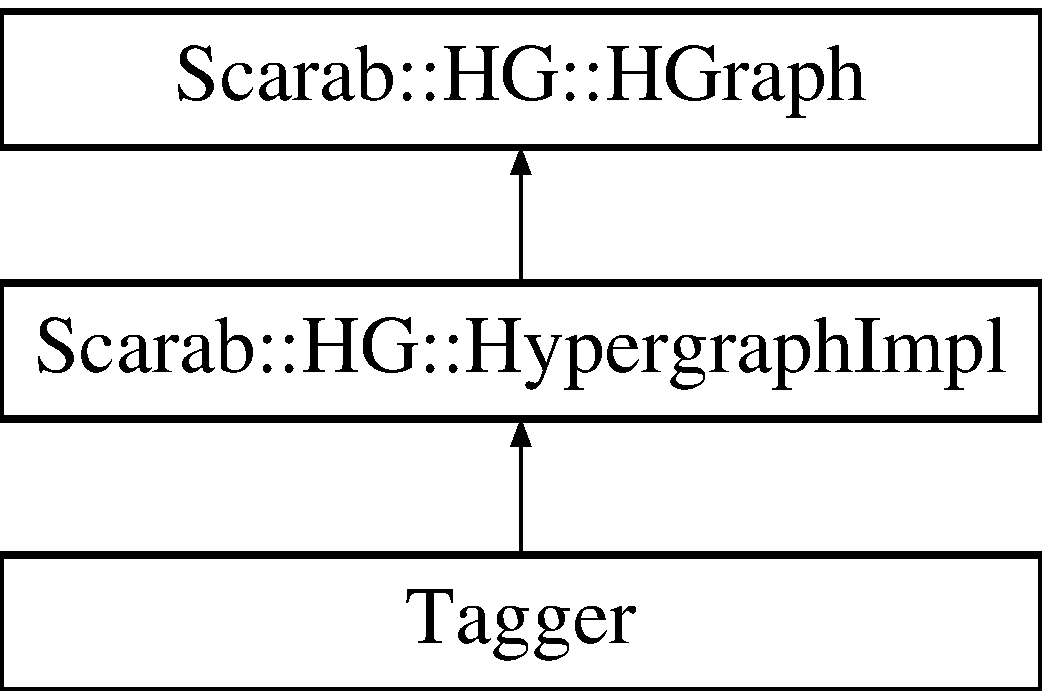
\includegraphics[height=3cm]{classTagger}
\end{center}
\end{figure}
\subsection*{Public Member Functions}
\begin{DoxyCompactItemize}
\item 
\hypertarget{classTagger_a6e812fd7e339a21155f7b30f04292be1}{
{\bfseries Tagger} (int num\_\-tags\_\-)}
\label{classTagger_a6e812fd7e339a21155f7b30f04292be1}

\item 
void \hyperlink{classTagger_a4ebe0aebd7c0392970b401a5a6c6cd72}{print} () const 
\item 
\hypertarget{classTagger_afafa6e435d17467db344ca615f24746f}{
void {\bfseries set\_\-up} (const Hypergraph \&hgraph)}
\label{classTagger_afafa6e435d17467db344ca615f24746f}

\item 
\hypertarget{classTagger_ad694ed218149b86c4ef5253328a41c49}{
const Hypergraph \& {\bfseries hypergraph} () const }
\label{classTagger_ad694ed218149b86c4ef5253328a41c49}

\item 
\hypertarget{classTagger_ae1e3802fb545c3430ca4d52ea5fd95db}{
vector$<$ \hyperlink{structTag}{Tag} $>$ {\bfseries tags} () const }
\label{classTagger_ae1e3802fb545c3430ca4d52ea5fd95db}

\item 
\hypertarget{classTagger_a5da221998377bf36c84013ba0d471b36}{
uint {\bfseries num\_\-tags} () const }
\label{classTagger_a5da221998377bf36c84013ba0d471b36}

\item 
\hypertarget{classTagger_ae762dd21f446b9ec618b0b83204bdc2e}{
uint {\bfseries sent\_\-length} () const }
\label{classTagger_ae762dd21f446b9ec618b0b83204bdc2e}

\item 
\hypertarget{classTagger_af01daf511528271a118a281b8595e0df}{
\hyperlink{structTag}{Tag} {\bfseries make\_\-tag} (int ind, int tag) const }
\label{classTagger_af01daf511528271a118a281b8595e0df}

\item 
\hypertarget{classTagger_a26472c386e7f5eebcb05c9d1843c1975}{
const vector$<$ const \hyperlink{classScarab_1_1HG_1_1Hyperedge}{Hyperedge} $\ast$ $>$ \& {\bfseries tag\_\-to\_\-edge} (const \hyperlink{structTag}{Tag} \&tag) const }
\label{classTagger_a26472c386e7f5eebcb05c9d1843c1975}

\item 
\hypertarget{classTagger_ae270a5be64b93945c180996aedcf6372}{
bool {\bfseries tag\_\-has\_\-edge} (const \hyperlink{structTag}{Tag} \&tag) const }
\label{classTagger_ae270a5be64b93945c180996aedcf6372}

\item 
\hypertarget{classTagger_ad615c8356f380baab01ae6675a25c409}{
const \hyperlink{structTag}{Tag} \& {\bfseries edge\_\-to\_\-tag} (const \hyperlink{classScarab_1_1HG_1_1Hyperedge}{Hyperedge} \&edge) const }
\label{classTagger_ad615c8356f380baab01ae6675a25c409}

\item 
\hypertarget{classTagger_ad7f1dda6082e71cd113a3d77e9c33275}{
bool {\bfseries edge\_\-has\_\-tag} (const \hyperlink{classScarab_1_1HG_1_1Hyperedge}{Hyperedge} \&edge) const }
\label{classTagger_ad7f1dda6082e71cd113a3d77e9c33275}

\end{DoxyCompactItemize}
\subsection*{Public Attributes}
\begin{DoxyCompactItemize}
\item 
\hypertarget{classTagger_a4bf3332c608c078cbb2d5692c4f13b43}{
int {\bfseries num\_\-tag}}
\label{classTagger_a4bf3332c608c078cbb2d5692c4f13b43}

\end{DoxyCompactItemize}
\subsection*{Protected Member Functions}
\begin{DoxyCompactItemize}
\item 
\hypertarget{classTagger_a305fd4cf75f2149a57109772e195eb47}{
void {\bfseries make\_\-edge} (const Hypergraph\_\-Edge \&edge, const \hyperlink{classScarab_1_1HG_1_1Hyperedge}{Scarab::HG::Hyperedge} $\ast$our\_\-edge)}
\label{classTagger_a305fd4cf75f2149a57109772e195eb47}

\end{DoxyCompactItemize}


\subsection{Member Function Documentation}
\hypertarget{classTagger_a4ebe0aebd7c0392970b401a5a6c6cd72}{
\index{Tagger@{Tagger}!print@{print}}
\index{print@{print}!Tagger@{Tagger}}
\subsubsection[{print}]{\setlength{\rightskip}{0pt plus 5cm}void Tagger::print () const\hspace{0.3cm}{\ttfamily  \mbox{[}inline, virtual\mbox{]}}}}
\label{classTagger_a4ebe0aebd7c0392970b401a5a6c6cd72}
Display the hypergraph for debugging. 

Implements \hyperlink{classScarab_1_1HG_1_1HGraph_ab5aa11c932b28864b56f28e0babbc1c1}{Scarab::HG::HGraph}.



The documentation for this class was generated from the following files:\begin{DoxyCompactItemize}
\item 
tagger/Tagger.h\item 
tagger/Tagger.cpp\end{DoxyCompactItemize}

\hypertarget{classTaggerDual}{
\section{TaggerDual Class Reference}
\label{classTaggerDual}\index{TaggerDual@{TaggerDual}}
}
Inheritance diagram for TaggerDual:\begin{figure}[H]
\begin{center}
\leavevmode
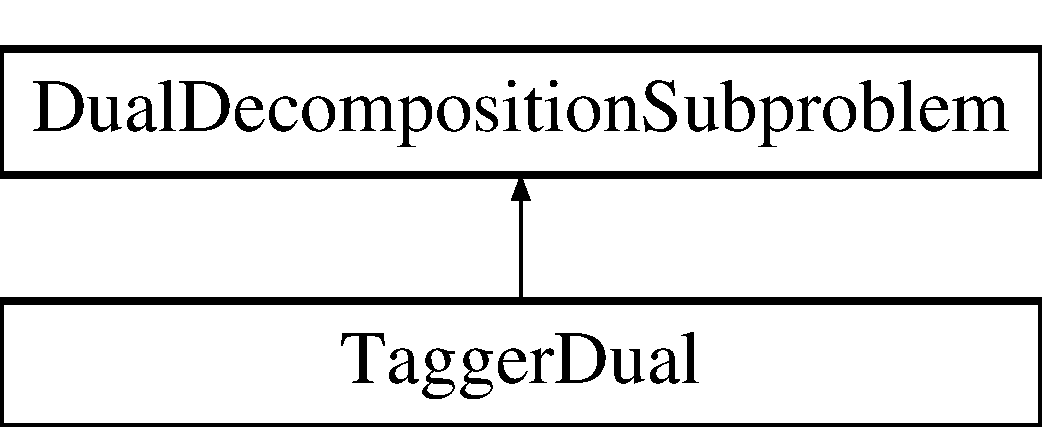
\includegraphics[height=2cm]{classTaggerDual}
\end{center}
\end{figure}
\subsection*{Public Member Functions}
\begin{DoxyCompactItemize}
\item 
\hypertarget{classTaggerDual_a2b16f45c3550e4f4871841c9ee02de4f}{
{\bfseries TaggerDual} (vector$<$ const \hyperlink{classTagger}{Tagger} $\ast$ $>$ \&taggers, const wvector \&base\_\-weights, const \hyperlink{classTagConstraints}{TagConstraints} \&cons)}
\label{classTaggerDual_a2b16f45c3550e4f4871841c9ee02de4f}

\item 
\hypertarget{classTaggerDual_a047785058d058492172280e50a8f4c1a}{
void {\bfseries solve} (double \&primal, double \&dual, wvector \&, int)}
\label{classTaggerDual_a047785058d058492172280e50a8f4c1a}

\item 
\hypertarget{classTaggerDual_a01f7705a69c7cc993268c6e66df57ae0}{
void {\bfseries update\_\-weights} (const wvector \&updates, wvector $\ast$weights, double mult)}
\label{classTaggerDual_a01f7705a69c7cc993268c6e66df57ae0}

\end{DoxyCompactItemize}
\subsection*{Protected Attributes}
\begin{DoxyCompactItemize}
\item 
\hypertarget{classTaggerDual_a0068b276abb09b34ab08e9cc14947ee3}{
const vector$<$ const \hyperlink{classTagger}{Tagger} $\ast$ $>$ \& {\bfseries \_\-taggers}}
\label{classTaggerDual_a0068b276abb09b34ab08e9cc14947ee3}

\item 
\hypertarget{classTaggerDual_a0073fa0f694790d365ca959ed8386e26}{
const wvector \& {\bfseries \_\-base\_\-weights}}
\label{classTaggerDual_a0073fa0f694790d365ca959ed8386e26}

\item 
\hypertarget{classTaggerDual_ab8845276b234c329c967529091f51e8f}{
const \hyperlink{classTagConstraints}{TagConstraints} \& {\bfseries \_\-tag\_\-constraints}}
\label{classTaggerDual_ab8845276b234c329c967529091f51e8f}

\item 
\hypertarget{classTaggerDual_a9974a79ebf2547f3e80e9d68d06b49be}{
wvector $\ast$ {\bfseries \_\-cur\_\-weights}}
\label{classTaggerDual_a9974a79ebf2547f3e80e9d68d06b49be}

\item 
\hypertarget{classTaggerDual_a57232f5a7702b7715f8517d408086dbe}{
vector$<$ wvector $>$ {\bfseries \_\-subgrad\_\-cache}}
\label{classTaggerDual_a57232f5a7702b7715f8517d408086dbe}

\item 
\hypertarget{classTaggerDual_a47cdc599b2c73836f33aa443053e3534}{
vector$<$ double $>$ {\bfseries \_\-primal\_\-cache}}
\label{classTaggerDual_a47cdc599b2c73836f33aa443053e3534}

\item 
\hypertarget{classTaggerDual_a4472c903ae391e7cc4912bc473a9eae2}{
vector$<$ double $>$ {\bfseries \_\-dual\_\-cache}}
\label{classTaggerDual_a4472c903ae391e7cc4912bc473a9eae2}

\item 
\hypertarget{classTaggerDual_a259d5ef5c5020c75a68527950ff41310}{
vector$<$ bool $>$ {\bfseries \_\-dirty\_\-cache}}
\label{classTaggerDual_a259d5ef5c5020c75a68527950ff41310}

\end{DoxyCompactItemize}


The documentation for this class was generated from the following files:\begin{DoxyCompactItemize}
\item 
tagger/TagSolvers.h\item 
tagger/TagSolvers.cpp\end{DoxyCompactItemize}

\hypertarget{classTagging}{
\section{Tagging Class Reference}
\label{classTagging}\index{Tagging@{Tagging}}
}
\subsection*{Public Member Functions}
\begin{DoxyCompactItemize}
\item 
\hypertarget{classTagging_a3236d0c0080d7f797f080151e66b756e}{
{\bfseries Tagging} (const \hyperlink{classTagging}{Tagging} \&from)}
\label{classTagging_a3236d0c0080d7f797f080151e66b756e}

\item 
\hypertarget{classTagging_ab21cdd0216e66fb17a8319c5f4b1a4d6}{
\hyperlink{classTagging}{Tagging} \& {\bfseries operator=} (const \hyperlink{classTagging}{Tagging} \&from)}
\label{classTagging_ab21cdd0216e66fb17a8319c5f4b1a4d6}

\item 
\hypertarget{classTagging_a1d1cc0a22c9a9f084b64f5fb6545390b}{
const ::google::protobuf::UnknownFieldSet \& {\bfseries unknown\_\-fields} () const }
\label{classTagging_a1d1cc0a22c9a9f084b64f5fb6545390b}

\item 
\hypertarget{classTagging_a91d117de804c4646ab9ea9d3103d40d9}{
inline::google::protobuf::UnknownFieldSet $\ast$ {\bfseries mutable\_\-unknown\_\-fields} ()}
\label{classTagging_a91d117de804c4646ab9ea9d3103d40d9}

\item 
\hypertarget{classTagging_a6b6767148366f94de9462d02171d19d0}{
void {\bfseries Swap} (\hyperlink{classTagging}{Tagging} $\ast$other)}
\label{classTagging_a6b6767148366f94de9462d02171d19d0}

\item 
\hypertarget{classTagging_ad46be5a72376294a63988a2662dc74b3}{
\hyperlink{classTagging}{Tagging} $\ast$ {\bfseries New} () const }
\label{classTagging_ad46be5a72376294a63988a2662dc74b3}

\item 
\hypertarget{classTagging_a337681fda513929c00d203798c04ad52}{
void {\bfseries CopyFrom} (const ::google::protobuf::Message \&from)}
\label{classTagging_a337681fda513929c00d203798c04ad52}

\item 
\hypertarget{classTagging_acaf751b83c2458013c2d12c4bdaea619}{
void {\bfseries MergeFrom} (const ::google::protobuf::Message \&from)}
\label{classTagging_acaf751b83c2458013c2d12c4bdaea619}

\item 
\hypertarget{classTagging_ab2271da80aa840cfa9b2de493b3eeb1f}{
void {\bfseries CopyFrom} (const \hyperlink{classTagging}{Tagging} \&from)}
\label{classTagging_ab2271da80aa840cfa9b2de493b3eeb1f}

\item 
\hypertarget{classTagging_a13d8b75c40ac5f295bc61a2f3f94c3b0}{
void {\bfseries MergeFrom} (const \hyperlink{classTagging}{Tagging} \&from)}
\label{classTagging_a13d8b75c40ac5f295bc61a2f3f94c3b0}

\item 
\hypertarget{classTagging_a43f8e265b50703f56a295083d3aa9676}{
void {\bfseries Clear} ()}
\label{classTagging_a43f8e265b50703f56a295083d3aa9676}

\item 
\hypertarget{classTagging_ab5617848ff03416f1ab4d98e2bfdef26}{
bool {\bfseries IsInitialized} () const }
\label{classTagging_ab5617848ff03416f1ab4d98e2bfdef26}

\item 
\hypertarget{classTagging_a6c2f74cb255bb4913fd279c6f3254729}{
int {\bfseries ByteSize} () const }
\label{classTagging_a6c2f74cb255bb4913fd279c6f3254729}

\item 
\hypertarget{classTagging_a1c8cf78b674f62c201f31e2b6ad721f2}{
bool {\bfseries MergePartialFromCodedStream} (::google::protobuf::io::CodedInputStream $\ast$input)}
\label{classTagging_a1c8cf78b674f62c201f31e2b6ad721f2}

\item 
\hypertarget{classTagging_afbd4d173621ed8cfc227dbcceec933d6}{
void {\bfseries SerializeWithCachedSizes} (::google::protobuf::io::CodedOutputStream $\ast$output) const }
\label{classTagging_afbd4d173621ed8cfc227dbcceec933d6}

\item 
\hypertarget{classTagging_a758bb0408c843056d4c70b917d02509b}{
::google::protobuf::uint8 $\ast$ {\bfseries SerializeWithCachedSizesToArray} (::google::protobuf::uint8 $\ast$output) const }
\label{classTagging_a758bb0408c843056d4c70b917d02509b}

\item 
\hypertarget{classTagging_a4661d58542895ed97b5e55ffb7d19f0c}{
int {\bfseries GetCachedSize} () const }
\label{classTagging_a4661d58542895ed97b5e55ffb7d19f0c}

\item 
\hypertarget{classTagging_a7d324ff2794e15d2c55c7238e173b520}{
::google::protobuf::Metadata {\bfseries GetMetadata} () const }
\label{classTagging_a7d324ff2794e15d2c55c7238e173b520}

\item 
\hypertarget{classTagging_a7e57b22b3a2162e380feae08233ee3a9}{
bool {\bfseries has\_\-ind} () const }
\label{classTagging_a7e57b22b3a2162e380feae08233ee3a9}

\item 
\hypertarget{classTagging_ad56efb939f57d519f4585a537c3d5266}{
void {\bfseries clear\_\-ind} ()}
\label{classTagging_ad56efb939f57d519f4585a537c3d5266}

\item 
\hypertarget{classTagging_ae6654e503f1906c0265012e311545c27}{
inline::google::protobuf::int32 {\bfseries ind} () const }
\label{classTagging_ae6654e503f1906c0265012e311545c27}

\item 
\hypertarget{classTagging_a34538a14f1727c2c15ddf43f5419f61b}{
void {\bfseries set\_\-ind} (::google::protobuf::int32 value)}
\label{classTagging_a34538a14f1727c2c15ddf43f5419f61b}

\item 
\hypertarget{classTagging_a8ef6eb12fffbe4fbd1b1fc622fc4fb87}{
bool {\bfseries has\_\-tag\_\-id} () const }
\label{classTagging_a8ef6eb12fffbe4fbd1b1fc622fc4fb87}

\item 
\hypertarget{classTagging_a25056abd232cdf45b153cb4b02b82dc2}{
void {\bfseries clear\_\-tag\_\-id} ()}
\label{classTagging_a25056abd232cdf45b153cb4b02b82dc2}

\item 
\hypertarget{classTagging_aa65105a209336790f3faf174b6e47813}{
inline::google::protobuf::int32 {\bfseries tag\_\-id} () const }
\label{classTagging_aa65105a209336790f3faf174b6e47813}

\item 
\hypertarget{classTagging_a44fc9490ab405218c27f13fa056b2ff5}{
void {\bfseries set\_\-tag\_\-id} (::google::protobuf::int32 value)}
\label{classTagging_a44fc9490ab405218c27f13fa056b2ff5}

\item 
\hypertarget{classTagging_a3236d0c0080d7f797f080151e66b756e}{
{\bfseries Tagging} (const \hyperlink{classTagging}{Tagging} \&from)}
\label{classTagging_a3236d0c0080d7f797f080151e66b756e}

\item 
\hypertarget{classTagging_ab21cdd0216e66fb17a8319c5f4b1a4d6}{
\hyperlink{classTagging}{Tagging} \& {\bfseries operator=} (const \hyperlink{classTagging}{Tagging} \&from)}
\label{classTagging_ab21cdd0216e66fb17a8319c5f4b1a4d6}

\item 
\hypertarget{classTagging_a1d1cc0a22c9a9f084b64f5fb6545390b}{
const ::google::protobuf::UnknownFieldSet \& {\bfseries unknown\_\-fields} () const }
\label{classTagging_a1d1cc0a22c9a9f084b64f5fb6545390b}

\item 
\hypertarget{classTagging_a91d117de804c4646ab9ea9d3103d40d9}{
inline::google::protobuf::UnknownFieldSet $\ast$ {\bfseries mutable\_\-unknown\_\-fields} ()}
\label{classTagging_a91d117de804c4646ab9ea9d3103d40d9}

\item 
\hypertarget{classTagging_a6b6767148366f94de9462d02171d19d0}{
void {\bfseries Swap} (\hyperlink{classTagging}{Tagging} $\ast$other)}
\label{classTagging_a6b6767148366f94de9462d02171d19d0}

\item 
\hypertarget{classTagging_ad46be5a72376294a63988a2662dc74b3}{
\hyperlink{classTagging}{Tagging} $\ast$ {\bfseries New} () const }
\label{classTagging_ad46be5a72376294a63988a2662dc74b3}

\item 
\hypertarget{classTagging_a337681fda513929c00d203798c04ad52}{
void {\bfseries CopyFrom} (const ::google::protobuf::Message \&from)}
\label{classTagging_a337681fda513929c00d203798c04ad52}

\item 
\hypertarget{classTagging_acaf751b83c2458013c2d12c4bdaea619}{
void {\bfseries MergeFrom} (const ::google::protobuf::Message \&from)}
\label{classTagging_acaf751b83c2458013c2d12c4bdaea619}

\item 
\hypertarget{classTagging_ab2271da80aa840cfa9b2de493b3eeb1f}{
void {\bfseries CopyFrom} (const \hyperlink{classTagging}{Tagging} \&from)}
\label{classTagging_ab2271da80aa840cfa9b2de493b3eeb1f}

\item 
\hypertarget{classTagging_a13d8b75c40ac5f295bc61a2f3f94c3b0}{
void {\bfseries MergeFrom} (const \hyperlink{classTagging}{Tagging} \&from)}
\label{classTagging_a13d8b75c40ac5f295bc61a2f3f94c3b0}

\item 
\hypertarget{classTagging_a43f8e265b50703f56a295083d3aa9676}{
void {\bfseries Clear} ()}
\label{classTagging_a43f8e265b50703f56a295083d3aa9676}

\item 
\hypertarget{classTagging_ab5617848ff03416f1ab4d98e2bfdef26}{
bool {\bfseries IsInitialized} () const }
\label{classTagging_ab5617848ff03416f1ab4d98e2bfdef26}

\item 
\hypertarget{classTagging_a6c2f74cb255bb4913fd279c6f3254729}{
int {\bfseries ByteSize} () const }
\label{classTagging_a6c2f74cb255bb4913fd279c6f3254729}

\item 
\hypertarget{classTagging_a1c8cf78b674f62c201f31e2b6ad721f2}{
bool {\bfseries MergePartialFromCodedStream} (::google::protobuf::io::CodedInputStream $\ast$input)}
\label{classTagging_a1c8cf78b674f62c201f31e2b6ad721f2}

\item 
\hypertarget{classTagging_afbd4d173621ed8cfc227dbcceec933d6}{
void {\bfseries SerializeWithCachedSizes} (::google::protobuf::io::CodedOutputStream $\ast$output) const }
\label{classTagging_afbd4d173621ed8cfc227dbcceec933d6}

\item 
\hypertarget{classTagging_a758bb0408c843056d4c70b917d02509b}{
::google::protobuf::uint8 $\ast$ {\bfseries SerializeWithCachedSizesToArray} (::google::protobuf::uint8 $\ast$output) const }
\label{classTagging_a758bb0408c843056d4c70b917d02509b}

\item 
\hypertarget{classTagging_a4661d58542895ed97b5e55ffb7d19f0c}{
int {\bfseries GetCachedSize} () const }
\label{classTagging_a4661d58542895ed97b5e55ffb7d19f0c}

\item 
\hypertarget{classTagging_a7d324ff2794e15d2c55c7238e173b520}{
::google::protobuf::Metadata {\bfseries GetMetadata} () const }
\label{classTagging_a7d324ff2794e15d2c55c7238e173b520}

\item 
\hypertarget{classTagging_a7e57b22b3a2162e380feae08233ee3a9}{
bool {\bfseries has\_\-ind} () const }
\label{classTagging_a7e57b22b3a2162e380feae08233ee3a9}

\item 
\hypertarget{classTagging_ad56efb939f57d519f4585a537c3d5266}{
void {\bfseries clear\_\-ind} ()}
\label{classTagging_ad56efb939f57d519f4585a537c3d5266}

\item 
\hypertarget{classTagging_a11022a65eecc2f9f771efb51e3414c59}{
inline::google::protobuf::int32 {\bfseries ind} () const }
\label{classTagging_a11022a65eecc2f9f771efb51e3414c59}

\item 
\hypertarget{classTagging_a34538a14f1727c2c15ddf43f5419f61b}{
void {\bfseries set\_\-ind} (::google::protobuf::int32 value)}
\label{classTagging_a34538a14f1727c2c15ddf43f5419f61b}

\item 
\hypertarget{classTagging_a8ef6eb12fffbe4fbd1b1fc622fc4fb87}{
bool {\bfseries has\_\-tag\_\-id} () const }
\label{classTagging_a8ef6eb12fffbe4fbd1b1fc622fc4fb87}

\item 
\hypertarget{classTagging_a25056abd232cdf45b153cb4b02b82dc2}{
void {\bfseries clear\_\-tag\_\-id} ()}
\label{classTagging_a25056abd232cdf45b153cb4b02b82dc2}

\item 
\hypertarget{classTagging_a2101441b351719ab45adde574a0e7255}{
inline::google::protobuf::int32 {\bfseries tag\_\-id} () const }
\label{classTagging_a2101441b351719ab45adde574a0e7255}

\item 
\hypertarget{classTagging_a44fc9490ab405218c27f13fa056b2ff5}{
void {\bfseries set\_\-tag\_\-id} (::google::protobuf::int32 value)}
\label{classTagging_a44fc9490ab405218c27f13fa056b2ff5}

\end{DoxyCompactItemize}
\subsection*{Static Public Member Functions}
\begin{DoxyCompactItemize}
\item 
\hypertarget{classTagging_a15430f96418c7b50335efcfe444c841f}{
static const ::google::protobuf::Descriptor $\ast$ {\bfseries descriptor} ()}
\label{classTagging_a15430f96418c7b50335efcfe444c841f}

\item 
\hypertarget{classTagging_a14f13d5d1d6489912bfc06ca67b484f7}{
static const \hyperlink{classTagging}{Tagging} \& {\bfseries default\_\-instance} ()}
\label{classTagging_a14f13d5d1d6489912bfc06ca67b484f7}

\item 
\hypertarget{classTagging_a15430f96418c7b50335efcfe444c841f}{
static const ::google::protobuf::Descriptor $\ast$ {\bfseries descriptor} ()}
\label{classTagging_a15430f96418c7b50335efcfe444c841f}

\item 
\hypertarget{classTagging_a14f13d5d1d6489912bfc06ca67b484f7}{
static const \hyperlink{classTagging}{Tagging} \& {\bfseries default\_\-instance} ()}
\label{classTagging_a14f13d5d1d6489912bfc06ca67b484f7}

\end{DoxyCompactItemize}
\subsection*{Static Public Attributes}
\begin{DoxyCompactItemize}
\item 
\hypertarget{classTagging_acd90c8d2f16535b6a8810a911a047274}{
static const int {\bfseries kIndFieldNumber} = 1}
\label{classTagging_acd90c8d2f16535b6a8810a911a047274}

\item 
\hypertarget{classTagging_aee9291b65c5317b5d58c9dfab2d0af6d}{
static const int {\bfseries kTagIdFieldNumber} = 2}
\label{classTagging_aee9291b65c5317b5d58c9dfab2d0af6d}

\end{DoxyCompactItemize}
\subsection*{Friends}
\begin{DoxyCompactItemize}
\item 
\hypertarget{classTagging_a5b6e1d0ac3f12cf6b846b7bc86f7fc96}{
void {\bfseries protobuf\_\-AddDesc\_\-tag\_\-2eproto} ()}
\label{classTagging_a5b6e1d0ac3f12cf6b846b7bc86f7fc96}

\item 
\hypertarget{classTagging_a84116f221ec83265dfdeb3bb01f9bd6c}{
void {\bfseries protobuf\_\-AssignDesc\_\-tag\_\-2eproto} ()}
\label{classTagging_a84116f221ec83265dfdeb3bb01f9bd6c}

\item 
\hypertarget{classTagging_a955ed450e7afd4065ffef15152e72563}{
void {\bfseries protobuf\_\-ShutdownFile\_\-tag\_\-2eproto} ()}
\label{classTagging_a955ed450e7afd4065ffef15152e72563}

\item 
\hypertarget{classTagging_a5b6e1d0ac3f12cf6b846b7bc86f7fc96}{
void {\bfseries protobuf\_\-AddDesc\_\-tag\_\-2eproto} ()}
\label{classTagging_a5b6e1d0ac3f12cf6b846b7bc86f7fc96}

\item 
\hypertarget{classTagging_a84116f221ec83265dfdeb3bb01f9bd6c}{
void {\bfseries protobuf\_\-AssignDesc\_\-tag\_\-2eproto} ()}
\label{classTagging_a84116f221ec83265dfdeb3bb01f9bd6c}

\item 
\hypertarget{classTagging_a955ed450e7afd4065ffef15152e72563}{
void {\bfseries protobuf\_\-ShutdownFile\_\-tag\_\-2eproto} ()}
\label{classTagging_a955ed450e7afd4065ffef15152e72563}

\end{DoxyCompactItemize}


The documentation for this class was generated from the following files:\begin{DoxyCompactItemize}
\item 
interfaces/hypergraph/gen-\/cpp/tag.pb.h\item 
interfaces/hypergraph/gen\_\-cpp/tag.pb.h\end{DoxyCompactItemize}

\hypertarget{structTagIndex}{
\section{TagIndex Struct Reference}
\label{structTagIndex}\index{TagIndex@{TagIndex}}
}
\subsection*{Public Member Functions}
\begin{DoxyCompactItemize}
\item 
\hypertarget{structTagIndex_a30a1bf326d593304ac3d950fd2b8be92}{
{\bfseries TagIndex} (int sent\_\-num\_\-, int ind\_\-, int tag\_\-)}
\label{structTagIndex_a30a1bf326d593304ac3d950fd2b8be92}

\item 
\hypertarget{structTagIndex_a7b858bbf2ed8ed6bb56d87db8d38aaf2}{
bool {\bfseries operator$<$} (const \hyperlink{structTagIndex}{TagIndex} \&other) const }
\label{structTagIndex_a7b858bbf2ed8ed6bb56d87db8d38aaf2}

\end{DoxyCompactItemize}
\subsection*{Public Attributes}
\begin{DoxyCompactItemize}
\item 
\hypertarget{structTagIndex_a9bde045f6de7e99933920b883af894dc}{
int {\bfseries sent\_\-num}}
\label{structTagIndex_a9bde045f6de7e99933920b883af894dc}

\item 
\hypertarget{structTagIndex_ac9cd159e647314e5beaf7af6da56fa6e}{
int {\bfseries ind}}
\label{structTagIndex_ac9cd159e647314e5beaf7af6da56fa6e}

\item 
\hypertarget{structTagIndex_a1182f316658b96f36ecd7689d790f508}{
POS {\bfseries tag}}
\label{structTagIndex_a1182f316658b96f36ecd7689d790f508}

\end{DoxyCompactItemize}


The documentation for this struct was generated from the following file:\begin{DoxyCompactItemize}
\item 
tagger/TagConstraints.h\end{DoxyCompactItemize}

\hypertarget{structScarab_1_1HG_1_1TagLP}{
\section{Scarab::HG::TagLP Struct Reference}
\label{structScarab_1_1HG_1_1TagLP}\index{Scarab::HG::TagLP@{Scarab::HG::TagLP}}
}
\subsection*{Public Member Functions}
\begin{DoxyCompactItemize}
\item 
\hypertarget{structScarab_1_1HG_1_1TagLP_a529942132dc8900bd25d2acaef721694}{
{\bfseries TagLP} (const \hyperlink{classTagger}{Tagger} \&parser, const \hyperlink{structScarab_1_1HG_1_1HypergraphLP}{HypergraphLP} \&hyper\_\-lp)}
\label{structScarab_1_1HG_1_1TagLP_a529942132dc8900bd25d2acaef721694}

\end{DoxyCompactItemize}
\subsection*{Public Attributes}
\begin{DoxyCompactItemize}
\item 
\hypertarget{structScarab_1_1HG_1_1TagLP_a4e80b783a5dfce94abb94cb957a3fe50}{
\hyperlink{classCache}{Cache}$<$ \hyperlink{structTag}{Tag}, GRBVar $>$ {\bfseries tag\_\-vars}}
\label{structScarab_1_1HG_1_1TagLP_a4e80b783a5dfce94abb94cb957a3fe50}

\item 
\hypertarget{structScarab_1_1HG_1_1TagLP_a137ec6055ea83b552c873dd19f203c15}{
const \hyperlink{classTagger}{Tagger} \& {\bfseries p}}
\label{structScarab_1_1HG_1_1TagLP_a137ec6055ea83b552c873dd19f203c15}

\item 
\hypertarget{structScarab_1_1HG_1_1TagLP_a92b885535389aa44e450e8f4682bf543}{
const \hyperlink{structScarab_1_1HG_1_1HypergraphLP}{HypergraphLP} \& {\bfseries h\_\-lp}}
\label{structScarab_1_1HG_1_1TagLP_a92b885535389aa44e450e8f4682bf543}

\end{DoxyCompactItemize}


The documentation for this struct was generated from the following file:\begin{DoxyCompactItemize}
\item 
lp/TagLP.h\end{DoxyCompactItemize}

\hypertarget{classScarab_1_1HG_1_1TagLPBuilder}{
\section{Scarab::HG::TagLPBuilder Class Reference}
\label{classScarab_1_1HG_1_1TagLPBuilder}\index{Scarab::HG::TagLPBuilder@{Scarab::HG::TagLPBuilder}}
}
\subsection*{Static Public Member Functions}
\begin{DoxyCompactItemize}
\item 
\hypertarget{classScarab_1_1HG_1_1TagLPBuilder_aa4990c224df5a1c82220a655ee51bd73}{
static void {\bfseries show\_\-results} (const \hyperlink{structScarab_1_1HG_1_1TagLP}{TagLP} \&lp\_\-vars)}
\label{classScarab_1_1HG_1_1TagLPBuilder_aa4990c224df5a1c82220a655ee51bd73}

\item 
\hypertarget{classScarab_1_1HG_1_1TagLPBuilder_a9c0f3ee542cbbed34945b80932272cea}{
static \hyperlink{structScarab_1_1HG_1_1TagLP}{TagLP} $\ast$ {\bfseries add\_\-tagging} (const \hyperlink{classTagger}{Tagger} \&parser, const \hyperlink{classCache}{Cache}$<$ \hyperlink{classScarab_1_1HG_1_1Hyperedge}{Hyperedge}, double $>$ \&weights, string prefix, GRBModel \&model, int var\_\-type)}
\label{classScarab_1_1HG_1_1TagLPBuilder_a9c0f3ee542cbbed34945b80932272cea}

\end{DoxyCompactItemize}


The documentation for this class was generated from the following files:\begin{DoxyCompactItemize}
\item 
lp/TagLP.h\item 
lp/TagLP.cpp\end{DoxyCompactItemize}

\hypertarget{classTagMrfAligner}{
\section{TagMrfAligner Class Reference}
\label{classTagMrfAligner}\index{TagMrfAligner@{TagMrfAligner}}
}
\subsection*{Public Member Functions}
\begin{DoxyCompactItemize}
\item 
\hypertarget{classTagMrfAligner_ae2bae21b52efb547b46f2da80f61ec42}{
void {\bfseries build\_\-from\_\-constraints} (string file\_\-name)}
\label{classTagMrfAligner_ae2bae21b52efb547b46f2da80f61ec42}

\item 
\hypertarget{classTagMrfAligner_a5b6ecf59596d656333f8113f6f05eba4}{
bool {\bfseries align} (\hyperlink{structTagIndex}{TagIndex} tag\_\-ind, \hyperlink{structMrfIndex}{MrfIndex} \&mrf\_\-ind)}
\label{classTagMrfAligner_a5b6ecf59596d656333f8113f6f05eba4}

\end{DoxyCompactItemize}
\subsection*{Public Attributes}
\begin{DoxyCompactItemize}
\item 
\hypertarget{classTagMrfAligner_a8a5d34bcfecdfb8c3901297ad34e301d}{
vector$<$ \hyperlink{classMRF}{MRF} $\ast$ $>$ {\bfseries mrf\_\-models}}
\label{classTagMrfAligner_a8a5d34bcfecdfb8c3901297ad34e301d}

\item 
\hypertarget{classTagMrfAligner_ae20f5a7d1131701986a36b70dca2c26f}{
vector$<$ vector$<$ \hyperlink{structTagIndex}{TagIndex} $>$ $>$ {\bfseries tag\_\-constraints}}
\label{classTagMrfAligner_ae20f5a7d1131701986a36b70dca2c26f}

\end{DoxyCompactItemize}


The documentation for this class was generated from the following files:\begin{DoxyCompactItemize}
\item 
tagger/TagConstraints.h\item 
tagger/TagConstraints.cpp\end{DoxyCompactItemize}

\hypertarget{classTagMrfLP}{
\section{TagMrfLP Class Reference}
\label{classTagMrfLP}\index{TagMrfLP@{TagMrfLP}}
}
\subsection*{Static Public Member Functions}
\begin{DoxyCompactItemize}
\item 
\hypertarget{classTagMrfLP_a7f9f963c533c5c712acca41db36f9a5a}{
static void {\bfseries align\_\-tag\_\-mrf} (const vector$<$ const \hyperlink{structMRFLP}{MRFLP} $\ast$ $>$ \&mrflp, const vector$<$ const \hyperlink{structScarab_1_1HG_1_1TagLP}{TagLP} $\ast$ $>$ \&taglp, \hyperlink{classTagMrfAligner}{TagMrfAligner} aligner, GRBModel \&model, int var\_\-type)}
\label{classTagMrfLP_a7f9f963c533c5c712acca41db36f9a5a}

\end{DoxyCompactItemize}


The documentation for this class was generated from the following file:\begin{DoxyCompactItemize}
\item 
lp/TagMrfLP.h\end{DoxyCompactItemize}

\printindex
\end{document}
